% Fichier genere par src/build.py -- ne pas modifier a la main
% =====================================================================
%  EPD-SDIA-4112 -- Statistique Bayesienne -- Master 1 SDIA
%  Preambule commun aux 5 chapitres
%  Moteur : XeLaTeX (Tectonic) -- compilation : voir build.py
% =====================================================================
\documentclass[10pt,aspectratio=169]{beamer}

\usepackage{fontspec}
\usepackage{polyglossia}
\setdefaultlanguage{french}
\usepackage{amsmath,amssymb,mathtools}
\usepackage{unicode-math}
\usepackage{booktabs}
\usepackage{array}
\usepackage{colortbl}
\usepackage{xcolor}
\usepackage{tikz}
\usetikzlibrary{arrows.meta,positioning,calc,shapes.geometric,fit,backgrounds,patterns}
\usepackage{pgfplots}
\pgfplotsset{compat=1.18}
\usepgfplotslibrary{fillbetween}
\usepackage{graphicx}
\usepackage{listings}
\usepackage[most]{tcolorbox}
\tcbuselibrary{skins,breakable}
\usepackage{fontawesome5}
\usepackage{multicol}
\usepackage{multirow}
\usepackage{animate}

% ---------------------------------------------------------------- theme
\usetheme{default}
\usecolortheme{default}
\setbeamertemplate{navigation symbols}{}

\definecolor{byDeep}   {HTML}{10243E}
\definecolor{byBlue}   {HTML}{1F6FEB}
\definecolor{byCyan}   {HTML}{12A594}
\definecolor{byOrange} {HTML}{D97706}
\definecolor{byRed}    {HTML}{C0392B}
\definecolor{byGreen}  {HTML}{1E8449}
\definecolor{byPurple} {HTML}{6C5CE7}
\definecolor{byGrey}   {HTML}{5B6470}
\definecolor{byLight}  {HTML}{F4F6F8}

\setbeamercolor{frametitle}{bg=byDeep,fg=white}
\setbeamercolor{structure}{fg=byBlue}
\setbeamercolor{normal text}{fg=byDeep}
\setbeamercolor{alerted text}{fg=byRed}
\setbeamercolor{title}{fg=white}
\setbeamercolor{subtitle}{fg=white}
\setbeamercolor{author}{fg=white}
\setbeamercolor{date}{fg=white}
\setbeamercolor{item}{fg=byBlue}
\setbeamercolor{section in toc}{fg=byDeep}
\setbeamercolor{block title}{bg=byBlue!12,fg=byDeep}
\setbeamercolor{block body}{bg=byBlue!5}

\setbeamerfont{frametitle}{size=\large,series=\bfseries}
\setbeamerfont{title}{size=\LARGE,series=\bfseries}
\setbeamerfont{block title}{series=\bfseries}

% gain de place vertical : le titre de frame est suivi d'un espace negatif
% (les supports sont denses ; cela evite que le dernier encadre morde sur le pied de page)
\addtobeamertemplate{frametitle}{}{\vspace*{-4.0mm}}
\setlength{\abovedisplayskip}{3pt}
\setlength{\belowdisplayskip}{3pt}
\setlength{\abovedisplayshortskip}{2pt}
\setlength{\belowdisplayshortskip}{2pt}

\setbeamertemplate{itemize item}{\small\raise0.2ex\hbox{\textcolor{byBlue}{$\blacktriangleright$}}}
\setbeamertemplate{itemize subitem}{\tiny\raise0.35ex\hbox{\textcolor{byCyan}{$\bullet$}}}
\setlength{\tabcolsep}{3pt}   % tableaux plus etroits (les slides sont denses)
% listes plus compactes : les supports sont denses et le pied de page mange de la place
\setbeamertemplate{itemize/enumerate body begin}{\vspace*{-2.0mm}}
\setbeamertemplate{itemize/enumerate subbody begin}{\vspace*{-0.6mm}}
\setbeamertemplate{enumerate item}{\textcolor{byBlue}{\bfseries\insertenumlabel.}}
\setbeamertemplate{caption}[numbered]

% footer : chapitre | slide n/N
\setbeamertemplate{footline}{%
  % Beamer reserve la hauteur de cette boite comme zone interdite : le vskip
  % ci-dessous cale la zone de texte exactement au-dessus de la barre visible.
  \vskip 10mm%
  \leavevmode%
  \hbox{%
    \begin{beamercolorbox}[wd=.42\paperwidth,ht=1.9ex,dp=0.8ex,leftskip=.3cm]{author in head/foot}%
      \usebeamerfont{author in head/foot}\color{white}\scriptsize\insertshorttitle
    \end{beamercolorbox}%
    \begin{beamercolorbox}[wd=.42\paperwidth,ht=1.9ex,dp=0.8ex,center]{title in head/foot}%
      \usebeamerfont{title in head/foot}\color{white}\scriptsize\insertsectionhead
    \end{beamercolorbox}%
    \begin{beamercolorbox}[wd=.16\paperwidth,ht=1.9ex,dp=0.8ex,rightskip=.3cm]{date in head/foot}%
      \usebeamerfont{date in head/foot}\color{white}\scriptsize\insertframenumber\,/\,\inserttotalframenumber
    \end{beamercolorbox}}%
  \vskip0pt%
}
\setbeamercolor{author in head/foot}{bg=byDeep}
\setbeamercolor{title in head/foot}{bg=byDeep!88}
\setbeamercolor{date in head/foot}{bg=byDeep!76}

\setbeamertemplate{title page}{%
  \begin{tikzpicture}[remember picture,overlay]
    \fill[byDeep] (current page.north west) rectangle (current page.south east);
    \fill[byBlue,opacity=.30] (current page.north east) ++(-3.2,-1.1) circle (5.4cm);
    \fill[byCyan,opacity=.18] (current page.south west) ++(2.2,1.0) circle (4.2cm);
  \end{tikzpicture}
  \vspace{1.1cm}
  \begin{center}
    {\usebeamerfont{title}\usebeamercolor[fg]{title}\inserttitle\par}
    \vspace{.25cm}
    {\large\color{byCyan}\insertsubtitle\par}
    \vspace{.7cm}
    {\color{white}\small\insertauthor\par}
    \vspace{.15cm}
    {\color{white!80}\footnotesize\insertinstitute\par}
    \vspace{.15cm}
    {\color{white!70}\footnotesize\insertdate\par}
  \end{center}
}

% ------------------------------------------------------- boites maison
\newtcolorbox{qbox}[1][QUIZ]{%
  enhanced,colback=byOrange!7,colframe=byOrange,boxrule=.9pt,arc=2mm,
  left=2mm,right=2mm,top=3.4mm,bottom=1.2mm,
  title={\faQuestionCircle\ \bfseries #1},fonttitle=\bfseries\scriptsize\color{white},
  colbacktitle=byOrange,attach boxed title to top left={xshift=3mm,yshift=-2mm},
  boxed title style={arc=1mm,boxrule=0pt}}

\newtcolorbox{abox}[1][ACTIVITE]{%
  enhanced,colback=byBlue!6,colframe=byBlue,boxrule=.9pt,arc=2mm,
  left=2mm,right=2mm,top=3.4mm,bottom=1.2mm,
  title={\faUsers\ \bfseries #1},fonttitle=\bfseries\scriptsize\color{white},
  colbacktitle=byBlue,attach boxed title to top left={xshift=3mm,yshift=-2mm},
  boxed title style={arc=1mm,boxrule=0pt}}

\newtcolorbox{ebox}[1][EXEMPLE]{%
  enhanced,colback=byGreen!6,colframe=byGreen,boxrule=.9pt,arc=2mm,
  left=2mm,right=2mm,top=3.4mm,bottom=1.2mm,
  title={\faFlask\ \bfseries #1},fonttitle=\bfseries\scriptsize\color{white},
  colbacktitle=byGreen,attach boxed title to top left={xshift=3mm,yshift=-2mm},
  boxed title style={arc=1mm,boxrule=0pt}}

\newtcolorbox{kbox}[1][A RETENIR]{%
  enhanced,colback=byPurple!6,colframe=byPurple,boxrule=.9pt,arc=2mm,
  left=2mm,right=2mm,top=3.4mm,bottom=1.2mm,
  title={\faLightbulb\ \bfseries #1},fonttitle=\bfseries\scriptsize\color{white},
  colbacktitle=byPurple,attach boxed title to top left={xshift=3mm,yshift=-2mm},
  boxed title style={arc=1mm,boxrule=0pt}}

\newtcolorbox{wbox}[1][ATTENTION]{%
  enhanced,colback=byRed!6,colframe=byRed,boxrule=.9pt,arc=2mm,
  left=2mm,right=2mm,top=3.4mm,bottom=1.2mm,
  title={\faExclamationTriangle\ \bfseries #1},fonttitle=\bfseries\scriptsize\color{white},
  colbacktitle=byRed,attach boxed title to top left={xshift=3mm,yshift=-2mm},
  boxed title style={arc=1mm,boxrule=0pt}}

\newtcolorbox{solbox}[1][SOLUTION]{%
  enhanced,colback=byCyan!7,colframe=byCyan,boxrule=.9pt,arc=2mm,
  left=2mm,right=2mm,top=3.4mm,bottom=1.2mm,
  title={\faCheckCircle\ \bfseries #1},fonttitle=\bfseries\scriptsize\color{white},
  colbacktitle=byCyan,attach boxed title to top left={xshift=3mm,yshift=-2mm},
  boxed title style={arc=1mm,boxrule=0pt}}

\newtcolorbox{codebox}[1][Code Python]{%
  enhanced,colback=byLight,colframe=byGrey!60,boxrule=.6pt,arc=1.5mm,
  left=1.5mm,right=1.5mm,top=3.8mm,bottom=1.0mm,
  title={\faPython\ \ttfamily\small #1},fonttitle=\small\color{white},
  colbacktitle=byGrey,attach boxed title to top left={xshift=3mm,yshift=-2mm},
  boxed title style={arc=1mm,boxrule=0pt}}

\newtcolorbox{figbox}[1][]{%
  enhanced,colback=white,colframe=byDeep!25,boxrule=.6pt,arc=1.5mm,
  left=1mm,right=1mm,top=1mm,bottom=1mm,#1}

% --------------------------------------------------------- listings
\definecolor{codekw}{HTML}{0B5394}
\definecolor{codestr}{HTML}{B8531A}
\definecolor{codecom}{HTML}{57744E}
\definecolor{codebg}{HTML}{F6F8FA}
\lstdefinestyle{py}{
  language=Python,
  backgroundcolor=\color{codebg},
  basicstyle=\ttfamily\fontsize{6.6}{7.6}\selectfont,
  keywordstyle=\color{codekw}\bfseries,
  commentstyle=\color{codecom}\itshape,
  stringstyle=\color{codestr},
  numberstyle=\tiny\color{byGrey},
  numbers=left,numbersep=4pt,
  frame=none,
  breaklines=true,breakatwhitespace=false,
  showstringspaces=false,
  columns=fullflexible,keepspaces=true,
  upquote=true,
  literate={é}{{\'e}}1 {è}{{\`e}}1 {ê}{{\^e}}1 {à}{{\`a}}1 {â}{{\^a}}1
           {î}{{\^i}}1 {ô}{{\^o}}1 {û}{{\^u}}1 {ç}{{\c c}}1 {ù}{{\`u}}1
           {É}{{\'E}}1 {È}{{\`E}}1 {À}{{\`A}}1 {Ê}{{\^E}}1 {Ç}{{\c C}}1
           {œ}{{\oe}}1 {’}{{'}}1 {«}{{\guillemotleft}}1 {»}{{\guillemotright}}1
           {→}{{$\rightarrow$}}1 {α}{{$\alpha$}}1 {β}{{$\beta$}}1 {θ}{{$\theta$}}1
           {μ}{{$\mu$}}1 {σ}{{$\sigma$}}1 {λ}{{$\lambda$}}1 {π}{{$\pi$}}1
           {τ}{{$\tau$}}1 {ρ}{{$\rho$}}1 {≈}{{$\approx$}}1 {≤}{{$\leq$}}1
           {≥}{{$\geq$}}1 {×}{{$\times$}}1 {≠}{{$\neq$}}1 {∈}{{$\in$}}1
}
\lstset{style=py}

\newcommand{\py}[1]{\lstinline[style=py,basicstyle=\ttfamily\small]|#1|}
\newcommand{\file}[1]{\texttt{\small #1}}
\newcommand{\R}{\mathbb{R}}
\newcommand{\N}{\mathcal{N}}
\newcommand{\E}{\mathbb{E}}
\newcommand{\Var}{\mathrm{Var}}
\newcommand{\post}{\text{post}}
\newcommand{\like}{\text{vrais.}}
\newcommand{\data}{\mathcal{D}}
\newcommand{\given}{\,\vert\,}
\DeclareMathOperator*{\argmax}{arg\,max}
\DeclareMathOperator*{\argmin}{arg\,min}

% icones de validation
\newcommand{\ok}{\textcolor{byGreen}{\faCheckCircle}}
\newcommand{\nok}{\textcolor{byRed}{\faTimesCircle}}
\newcommand{\warn}{\textcolor{byOrange}{\faExclamationTriangle}}

% chemin des figures
\graphicspath{{../figures/}{./figures/}{figures/}{../assets/}{./assets/}}

% ------------------------------------------------ page de garde de chapitre
% A utiliser en tete de chaque fichier de chapitre : identique en build
% autonome et en build maitre (aucune dependance a \title).
\newcommand{\chapterslide}[4]{%
\begin{frame}[plain]
\begin{tikzpicture}[remember picture,overlay]
  \fill[byDeep] (current page.north west) rectangle (current page.south east);
  \fill[byBlue,opacity=.30] (current page.north east) ++(-3.0,-0.9) circle (5.0cm);
  \fill[byCyan,opacity=.16] (current page.south west) ++(2.4,1.2) circle (4.4cm);
\end{tikzpicture}
\vspace{0.55cm}
\begin{columns}[c]
% ---- logo officiel de l'ecole, dans un cartouche blanc
\begin{column}{0.20\textwidth}
  \centering
  \begin{tcolorbox}[colback=white,colframe=white,boxrule=0pt,arc=1.5mm,
     left=1mm,right=1mm,top=1mm,bottom=1mm,width=2.5cm]
    \centering
    
\includegraphics[width=2.1cm]{logo_enspd.png}
  \end{tcolorbox}
\end{column}
% ---- identification du chapitre et de l'enseignante
\begin{column}{0.76\textwidth}
  {\color{byCyan}\bfseries\large #1\par}
  \vspace{.20cm}
  {\color{white}\bfseries\Large #2\par}
  \vspace{.30cm}
  {\color{white!85}\small Statistique Bayésienne --- EPD-SDIA-4112 --- Master 1 SDIA\par}
  \vspace{.06cm}
  {\color{white!70}\footnotesize #3\par}
  \vspace{.26cm}
  {\color{byCyan}\bfseries\normalsize Enseignante : Dr. Noulapeu Ngaffo Armielle\par}
  \vspace{.06cm}
  {\color{white!80}\footnotesize École Nationale Supérieure Polytechnique de Douala\par}
  {\color{white!65}\footnotesize Université de Douala --- Département Génie Informatique
   et Télécommunications\par}
\end{column}
\end{columns}
\vspace{.30cm}
\begin{columns}[t]
\begin{column}{0.06\textwidth}\end{column}
\begin{column}{0.88\textwidth}
\begin{tcolorbox}[enhanced,colback=byDeep!62!black,colframe=byCyan!75,arc=2mm,
   boxrule=.6pt,left=2mm,right=2mm,top=1.4mm,bottom=1.4mm,coltext=white]
\small #4
\end{tcolorbox}
\end{column}
\begin{column}{0.06\textwidth}\end{column}
\end{columns}
\end{frame}}

% compteur de slides atteignables : \nb{50}
\newcommand{\nb}[1]{}


\title[Cours complet]{Statistique Bayésienne --- support complet}
\subtitle{EPD-SDIA-4112 --- Master 1 Science des Données et Intelligence Artificielle}
\author{Enseignante : Dr. Noulapeu Ngaffo Armielle}
\institute{Département Génie Informatique et Télécommunications}
\date{Année universitaire 2026--2027}
\begin{document}
% =====================================================================
%  EPD-SDIA-4112 -- Statistique Bayesienne -- Master 1 SDIA
%  CHAPITRE 1 : Introduction et fondements bayesiens   (50 slides, 8 h)
%  Fichier de frames : aucune dependance a \title (build maitre + build seul)
% =====================================================================
\section{Chapitre 1 --- Fondements bayésiens}

% ---------------------------------------------------------------- 1
\chapterslide{Chapitre 1}{Introduction et fondements bayésiens}{8 h --- 5 sections --- 50 slides}{%
\textbf{Objectifs} --- distinguer les deux interprétations de la probabilité ;
énoncer et appliquer le théorème de Bayes ; définir prior, vraisemblance,
posterior et loi prédictive ; écrire un premier modèle en PyMC ;
lire un intervalle de crédibilité à 95~\%.}


% ---------------------------------------------------------------- 2
\begin{frame}{Pourquoi le bayésien ?}
\begin{columns}[t]
\begin{column}{0.52\textwidth}
\begin{ebox}[Trois raisons décisives]
\begin{itemize}
  \item \textbf{Données rares} : en santé, finance ou industrie, on ne dispose
        pas de 10\,000 observations. Le prior compense.
  \item \textbf{Connaissance experte} : l'expert sait déjà quelque chose ;
        le bayésien lui donne un langage pour l'écrire.
  \item \textbf{Incertitude honnête} : on répond par
        « $P(\theta > 0{,}5 \given y) = 0{,}97$ », pas par un rejet binaire.
\end{itemize}
\end{ebox}
\end{column}
\begin{column}{0.44\textwidth}
\begin{kbox}[Applications en M1 SDIA]
\begin{itemize}
  \item Dépistage et essais cliniques
  \item A/B testing en ligne
  \item Filtrage de spam, détection de fraude
  \item Systèmes de recommandation
  \item Modèles hiérarchiques et petits effectifs
  \item Apprentissage bayésien profond (BNN)
\end{itemize}
\end{kbox}
\end{column}
\end{columns}
\vspace{1mm}
\centering
\begin{tcolorbox}[colback=byCyan!8,colframe=byCyan,width=.94\textwidth,arc=2mm]
\centering\small
\textbf{Fil rouge du cours :} transformer une croyance a priori en
\textbf{distribution de probabilité} sur le paramètre, puis la mettre à jour par les données.
\end{tcolorbox}
\end{frame}

% ---------------------------------------------------------------- 3
\begin{frame}{Le problème qui met tout le monde d'accord}
\begin{columns}[t]
\begin{column}{0.48\textwidth}
\begin{ebox}[Énoncé]
Un test de dépistage a
\begin{itemize}
  \item sensibilité $P(T^+ \given M) = 0{,}99$
  \item spécificité $P(T^- \given \bar M) = 0{,}95$
  \item maladie rare : prévalence $P(M) = 0{,}01$
\end{itemize}
\vspace{1mm}
\textbf{Question :} le test est positif. Quelle est la probabilité d'être malade ?
\vspace{1mm}

\centering\large\textbf{Réponse intuitive la plus fréquente : 95 \%}
\end{ebox}
\end{column}
\begin{column}{0.48\textwidth}
\begin{center}
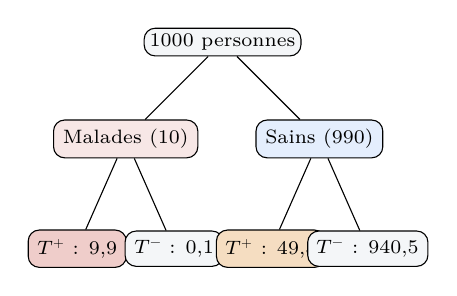
\begin{tikzpicture}[scale=.82,every node/.style={font=\scriptsize},
   level 1/.style={sibling distance=30mm,level distance=15mm},
   level 2/.style={sibling distance=15mm,level distance=17mm}]
\node[draw,rounded corners,fill=byLight,inner sep=2pt] {1000 personnes}
  child {node[draw,rounded corners,fill=byRed!12] {Malades (10)}
    child {node[fill=byRed!25,draw,rounded corners] {$T^+$ : 9,9}}
    child {node[fill=byLight,draw,rounded corners] {$T^-$ : 0,1}}}
  child {node[draw,rounded corners,fill=byBlue!12] {Sains (990)}
    child {node[fill=byOrange!25,draw,rounded corners] {$T^+$ : 49,5}}
    child {node[fill=byLight,draw,rounded corners] {$T^-$ : 940,5}}};
\end{tikzpicture}
\end{center}
\vspace{-1mm}
\begin{solbox}[Le calcul qui fâche]
\centering
$P(M \given T^+) = \dfrac{9{,}9}{9{,}9 + 49{,}5} = \mathbf{16{,}7\ \%}$
\end{solbox}
\end{column}
\end{columns}
\end{frame}

% ---------------------------------------------------------------- 4
\begin{frame}{Quiz d'ouverture (Kahoot / Mentimeter, 3 min)}
\begin{qbox}[Question 1 -- Diagnostic médical]
Même test (sensibilité 99 \%, spécificité 95 \%). La prévalence passe de 1 \% à 20 \%.
Quelle est la nouvelle probabilité d'être malade après un test positif ?
\vspace{2mm}
\begin{enumerate}
  \item[(A)] environ 17 \% \quad \textit{(inchangé : le test est le même)}
  \item[(B)] environ 83 \% \quad \checkmark
  \item[(C)] environ 99 \%
  \item[(D)] impossible à dire sans plus de données
\end{enumerate}
\vspace{2mm}
\textcolor{byBlue}{\textbf{Votez avant de calculer.}} Puis :
$P(M \given T^+) = \frac{0{,}99 \times 0{,}20}{0{,}99 \times 0{,}20 + 0{,}05 \times 0{,}80} = 0{,}832$.
\end{qbox}
\vspace{1mm}
\begin{kbox}[Le message de la séance]
La réponse ne dépend pas seulement du test : elle dépend de ce qu'on
\textbf{croyait avant}. C'est toute la statistique bayésienne en une phrase.
\end{kbox}
\end{frame}

% ---------------------------------------------------------------- 5
\begin{frame}{Trois siècles d'une idée contrariée}
\begin{center}
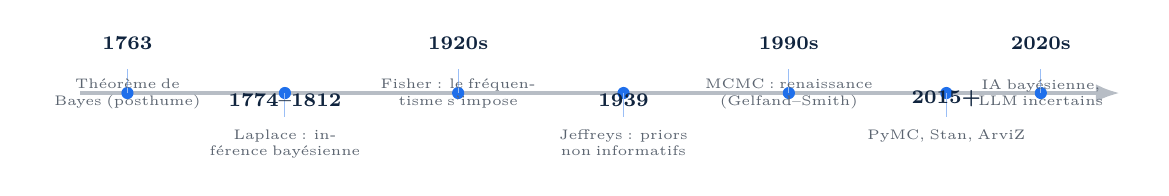
\begin{tikzpicture}[xscale=1.0,yscale=1.0]
\draw[very thick,byDeep!30,-{Latex[length=3mm]}] (0,0) -- (13.2,0);
\foreach \x/\y/\n/\t in {
   0.6/1/{1763}/{Théorème de Bayes (posthume)},
   2.6/-1/{1774--1812}/{Laplace : inférence bayésienne},
   4.8/1/{1920s}/{Fisher : le fréquentisme s'impose},
   6.9/-1/{1939}/{Jeffreys : priors non informatifs},
   9.0/1/{1990s}/{MCMC : renaissance (Gelfand--Smith)},
   11.0/-1/{2015+}/{PyMC, Stan, ArviZ},
   12.2/1/{2020s}/{IA bayésienne, LLM incertains}}
{
  \fill[byBlue] (\x,0) circle (2.2pt);
  \draw[byBlue!45] (\x,0) -- (\x,0.30*\y+0.0);
  \node[anchor=south,align=center,font=\scriptsize\bfseries,text=byDeep]
       at (\x,0.36*\y+0.06) {\n};
  \node[anchor=north,align=center,font=\tiny,text=byGrey,text width=2.3cm]
       at (\x,0.32*\y-0.02) {\t};
}
\end{tikzpicture}
\end{center}
\vspace{2mm}
\begin{ebox}[Pourquoi si longtemps ?]
\begin{itemize}
  \item Le calcul bayésien exige des intégrales $\int p(\theta) p(y \given \theta)\,\mathrm{d}\theta$,
        souvent sans forme close.
  \item Les ordinateurs et les algorithmes MCMC (chapitre 5) ont levé ce verrou
        \textbf{à la fin des années 1980}.
  \item Aujourd'hui une régression bayésienne tient en cinq lignes de \py{pm.sample()}.
\end{itemize}
\end{ebox}
\end{frame}

% ---------------------------------------------------------------- 6
\begin{frame}{Objectifs pédagogiques du chapitre}
\begin{columns}[t]
\begin{column}{0.48\textwidth}
\begin{kbox}[Savoirs]
\begin{itemize}
  \item Distinguer les deux interprétations de la probabilité
  \item Énoncer et démontrer le théorème de Bayes
  \item Définir prior, vraisemblance, posterior, prédictive
  \item Lire un intervalle de crédibilité
\end{itemize}
\end{kbox}
\end{column}
\begin{column}{0.48\textwidth}
\begin{abox}[Savoir-faire évalués]
\begin{itemize}
  \item Calculer un posterior conjugué à la main
  \item \textbf{Écrire et exécuter} un modèle PyMC
  \item Produire un graphique de posterior exploitable
  \item Critiquer un prior (trop informatif ? justifié ?)
\end{itemize}
\end{abox}
\end{column}
\end{columns}
\vspace{2mm}
\begin{tcolorbox}[colback=byLight,colframe=byGrey!50,arc=2mm,width=.95\textwidth]
\centering\small
\textbf{Évaluation} — contrôle continu 30 \% (TP noté + quiz) \;|\; examen final écrit 70 \%.
\end{tcolorbox}
\end{frame}

% ---------------------------------------------------------------- 7
\begin{frame}{Plan du chapitre 1 (8 h)}
\begin{enumerate}
  \item[1.1] \textbf{Contexte et motivation} \hfill \textit{slides 2--8}
  \item[1.2] \textbf{Probabilité : deux interprétations} \hfill \textit{slides 9--20}
  \item[1.3] \textbf{Le théorème de Bayes et sa mécanique} \hfill \textit{slides 21--34}
  \item[1.4] \textbf{Bayésien contre fréquentiste} \hfill \textit{slides 35--44}
  \item[1.5] \textbf{L'écosystème logiciel et le premier modèle} \hfill \textit{slides 45--50}
\end{enumerate}
\vspace{3mm}
\begin{tabular}{@{}llll@{}}
\toprule
\textbf{Volume} & \textbf{Cours magistral} & \textbf{TD} & \textbf{TP machine} \\
\midrule
8 h & 5 h & 1 h 30 & 1 h 30 \\
\bottomrule
\end{tabular}
\vspace{2mm}
\begin{tcolorbox}[colback=byPurple!6,colframe=byPurple,arc=2mm,width=.95\textwidth]
\small\centering
\textbf{Prérequis mobilisés} : probabilités conditionnelles, loi binomiale et normale,
$\int_0^1 x^{a-1}(1-x)^{b-1}\mathrm{d}x$, Python.
\end{tcolorbox}
\end{frame}

% ---------------------------------------------------------------- 8
\begin{frame}{Activité brise-glace — tour de table (5 min)}
\begin{abox}[Consigne]
Chacun cite \textbf{une décision incertaine} de son domaine, en une phrase, puis indique
\textbf{ce qu'il savait déjà} avant de voir les données.
\end{abox}
\vspace{1mm}
\begin{columns}[t]
\begin{column}{0.31\textwidth}
\begin{ebox}[Santé]
« Ce traitement marche-t-il sur 12 patients ? »
\vspace{1mm}
\footnotesize Ce qu'on sait : les essais antérieurs, la physiologie.
\end{ebox}
\end{column}
\begin{column}{0.31\textwidth}
\begin{ebox}[Industrie / Web]
« Ce bouton augmente-t-il le taux de clic ? »
\vspace{1mm}
\footnotesize Ce qu'on sait : les A/B tests passés, la taille d'effet plausible.
\end{ebox}
\end{column}
\begin{column}{0.31\textwidth}
\begin{ebox}[Recommandation]
« Ce film va-t-il plaire ? »
\vspace{1mm}
\footnotesize Ce qu'on sait : les goûts déclarés, les notes globales.
\end{ebox}
\end{column}
\end{columns}
\vspace{2mm}
\begin{kbox}[Ce que l'on va apprendre à faire]
Transformer la colonne « ce qu'on sait » en une \textbf{loi a priori}, puis la
confronter aux données sans jeter ni l'un ni l'autre.
\end{kbox}
\end{frame}

% ---------------------------------------------------------------- 9
\begin{frame}{Deux visions de la probabilité}
\begin{columns}[t]
\begin{column}{0.48\textwidth}
\begin{tcolorbox}[enhanced,colback=byRed!7,colframe=byRed,arc=2mm,
   title={\bfseries\color{white} Fréquentiste},colbacktitle=byRed,
   attach boxed title to top left={xshift=3mm,yshift=-2mm},
   boxed title style={arc=1mm,boxrule=0pt}]
\begin{itemize}
  \item Probabilité = \textbf{fréquence de long terme} d'un événement répétable
  \item Le paramètre $\theta$ est \textbf{fixe et inconnu}
  \item On raisonne sur la variabilité des \textbf{échantillons}
  \item Outils : $p$-value, intervalle de confiance, puissance
  \item Phrase type : « si je répétais 1000 fois l'expérience, dans 95 \% des cas… »
\end{itemize}
\end{tcolorbox}
\end{column}
\begin{column}{0.48\textwidth}
\begin{tcolorbox}[enhanced,colback=byBlue!7,colframe=byBlue,arc=2mm,
   title={\bfseries\color{white} Bayésien},colbacktitle=byBlue,
   attach boxed title to top left={xshift=3mm,yshift=-2mm},
   boxed title style={arc=1mm,boxrule=0pt}]
\begin{itemize}
  \item Probabilité = \textbf{degré de croyance} cohérent (\textit{plausibilité})
  \item Le paramètre $\theta$ est \textbf{aléatoire}, décrit par une loi
  \item On raisonne sur la variabilité du \textbf{paramètre}
  \item Outils : distribution a posteriori, intervalle de crédibilité
  \item Phrase type : « il y a 95 \% de chance que $\theta$ soit dans… »
\end{itemize}
\end{tcolorbox}
\end{column}
\end{columns}
\vspace{1.5mm}
\centering\small
Les deux écoles utilisent \textbf{les mêmes probabilités conditionnelles} :
elles diffèrent sur \textit{ce qui est aléatoire}.
\end{frame}

% ---------------------------------------------------------------- 10
% [split]
\begin{frame}{Ce que dit une fréquence, et ce qu'elle ne dit pas}
\begin{center}
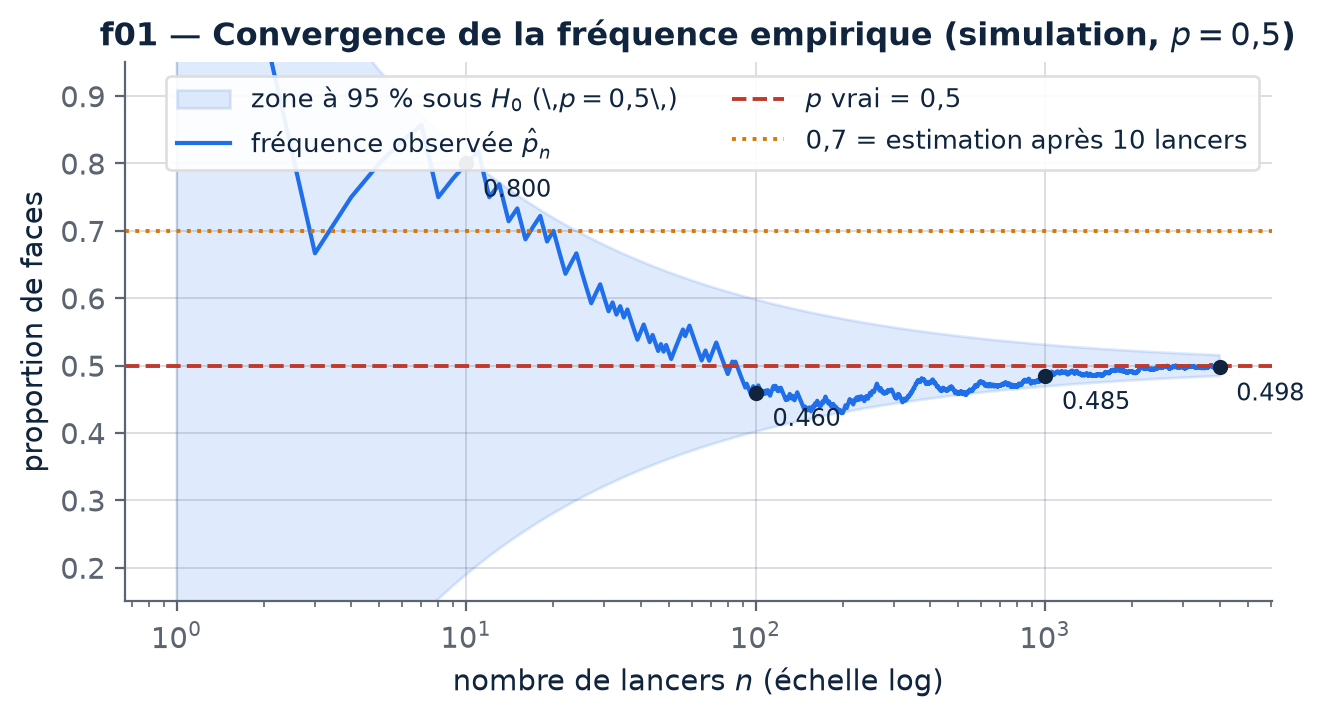
\includegraphics[width=.86\textwidth]{f01_convergence_frequence.png}
\end{center}
\end{frame}

% [split]
\begin{frame}{Ce que dit une fréquence, et ce qu'elle ne dit pas}

\vspace{-1mm}
\begin{columns}[t]
\begin{column}{0.54\textwidth}
\begin{ebox}[Lecture des données simulées]
Après 10 lancers on observe $\hat p = $ \textbf{0,80}. Après 4000 lancers : \textbf{0,498}.
Le fréquentiste conclut : \emph{« la fréquence converge vers $p$ ; la valeur
0,80 n'est qu'une fluctuation »} — mais il ne peut pas parler de $P(0{,}45 < p < 0{,}55)$\dots
\end{ebox}
\end{column}
\begin{column}{0.42\textwidth}
\begin{wbox}[Le piège fréquentiste]
\begin{itemize}
  \item $p$ n'est pas une variable : aucune probabilité ne lui est attachée.
  \item L'IC à 95 \% est \textbf{un long terme théorique}, pas la confiance dans
        \emph{cet} intervalle calculé.
  \item Aucun moyen d'injecter le fait que la pièce semble équilibrée \textit{a priori}.
\end{itemize}
\end{wbox}
\end{column}
\end{columns}
\end{frame}

% ---------------------------------------------------------------- 11
\begin{frame}{La probabilité comme état de connaissance}
\begin{kbox}[Postulat bayésien]
Une probabilité est une \textbf{appréciation de plausibilité par un agent} cohérent.
Deux agents avec des informations différentes \emph{doivent} avoir des probabilités
différentes — et c'est une force, à condition de dire lesquelles.
\end{kbox}
\vspace{2mm}
\begin{columns}[t]
\begin{column}{0.48\textwidth}
\begin{ebox}[Exemple 1 — question piégée]
« Quelle est la probabilité que la Chine soit le premier pays à poser un humain sur Mars ? »
\vspace{1mm}
\footnotesize Il n'y a pas de « fréquence de long terme » : l'événement est unique.
Pourtant on sait raisonner, comparer, mettre à jour.
\end{ebox}
\end{column}
\begin{column}{0.48\textwidth}
\begin{ebox}[Exemple 2 — l'ordre]
« Ce patient a survécu 3 mois au traitement. »
\vspace{1mm}
\footnotesize Le bayésien peut arrêter l'essai quand les données le justifient
(interprétation \textit{conditionnelle} aux données observées),
sans gonfler artificiellement le risque de première espèce.
\end{ebox}
\end{column}
\end{columns}
\vspace{1.5mm}
\begin{tcolorbox}[colback=byCyan!8,colframe=byCyan,arc=2mm,width=.95\textwidth]
\small\centering
\textbf{Conséquence pratique :} la conclusion bayésienne s'énonce
\textbf{conditionnellement aux données réellement observées} — pas sur des
répétitions imaginaires de l'expérience.
\end{tcolorbox}
\end{frame}

% ---------------------------------------------------------------- 12
\begin{frame}{Mise à jour séquentielle : le cœur du raisonnement}
\begin{ebox}[Principe]
Le posterior d'aujourd'hui devient le prior de demain :
$p(\theta \given y_1, y_2) \neq$ refaire tout le calcul, mais
$p(\theta \given y_1, y_2) \propto p(\theta) \, p(y_1 \given \theta) \, p(y_2 \given \theta)$.
L'ordre d'arrivée des données \textbf{ne change pas} le résultat.
\end{ebox}
\vspace{1mm}
\begin{center}
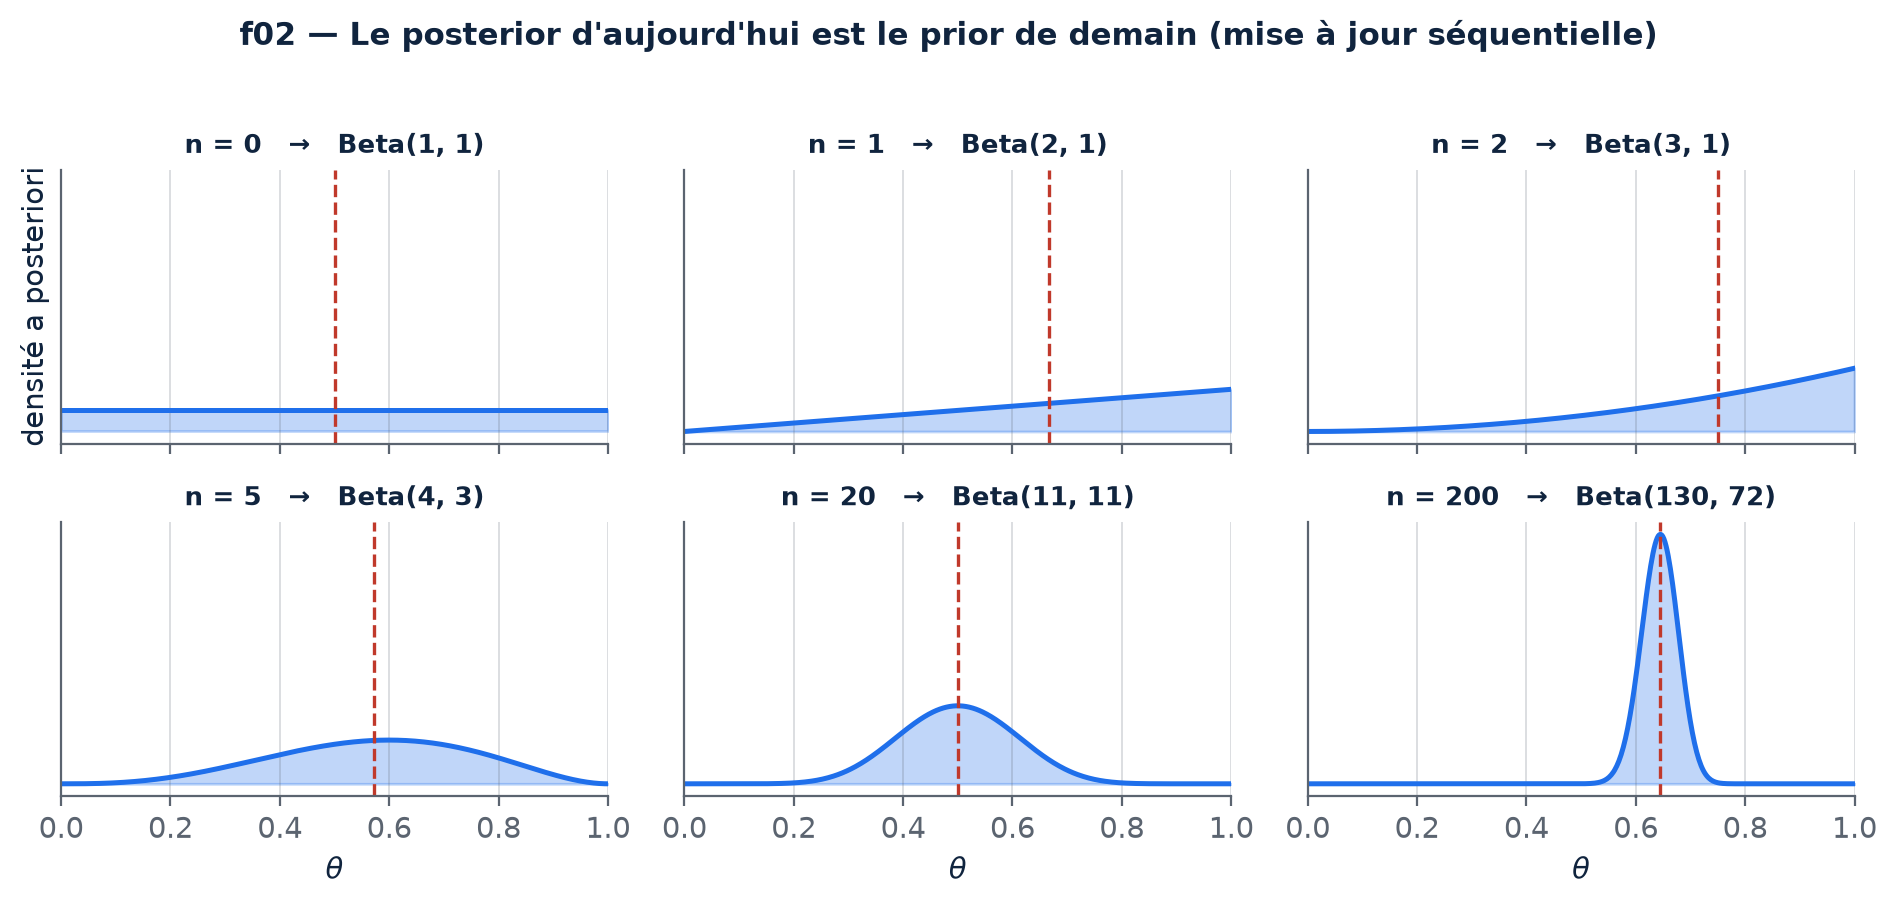
\includegraphics[width=.82\textwidth]{f02_beta_updating.png}
\end{center}
\vspace{-1mm}
\centering\footnotesize
Simulation réelle : 200 lancers d'une pièce biaisée ($p = 0{,}65$), prior Beta$(1,1)$.
La dispersion se resserre comme $1/\sqrt{n}$ : c'est la \emph{vitesse d'apprentissage}.
\end{frame}

% ---------------------------------------------------------------- 13
\begin{frame}{Vocabulaire : quatre objets, un raisonnement}
\begin{center}
{\setlength{\tabcolsep}{3pt}\begin{tabular}{@{}p{2.0cm}p{2.5cm}p{4.2cm}p{4.3cm}@{}}
\toprule
\textbf{Objet} & \textbf{Notation} & \textbf{Interprétation} & \textbf{Exemple (pièce biaisée)} \\
\midrule
A priori & $p(\theta)$ & ce que l'on croit \emph{avant} les données &
Beta$(2,2)$ : « la pièce est plausiblement équilibrée » \\[2mm]
Vraisemblance & $p(y \given \theta)$ & probabilité des données \emph{si} le paramètre valait $\theta$ &
Bin$\big(10, \theta\big)$ : 7 faces sur 10 \\[2mm]
A posteriori & $p(\theta \given y)$ & la croyance \emph{après} les données &
Beta$(9,5)$ : centré sur 0,64 \\[2mm]
Prédictive & $p(\tilde y \given y)$ & ce qu'on attend de la prochaine observation &
$P(\text{face}) = \int \theta\, p(\theta \given y)\,\mathrm{d}\theta = 0{,}643$ \\
\bottomrule
\end{tabular}}
\end{center}
\vspace{1mm}
\begin{kbox}[La règle d'or]
Le prior est \textbf{ce qu'on met sur la table} ; le posterior est
\textbf{ce qui en reste après avoir vu les données}. Rien ne se perd, tout se met à jour.
\end{kbox}
\end{frame}

% ---------------------------------------------------------------- 14
\begin{frame}{Exemple fondateur : la pièce truquée --- l'énoncé}
\begin{ebox}[Énoncé]
On lance 10 fois une pièce et on obtient \textbf{7 faces}.
\begin{itemize}
  \item Paramètre : $\theta = P(\text{face}) \in [0,1]$
  \item Prior : $\theta \sim \mathrm{Beta}(1,1)$ (uniforme)
  \item Vraisemblance : $y \given \theta \sim \mathrm{Bin}(10, \theta)$
\end{itemize}
\vspace{1mm}
\textbf{Questions}
\begin{enumerate}
  \item Forme du posterior ?
  \item Valeur centrale ?
  \item Intervalle de crédibilité à 95 \% ?
  \item $P(\theta > 0{,}5 \given y)$ ?
\end{enumerate}
\end{ebox}
\end{frame}

% [split]
\begin{frame}{Exemple fondateur : la pièce truquée --- le posterior}
\begin{center}
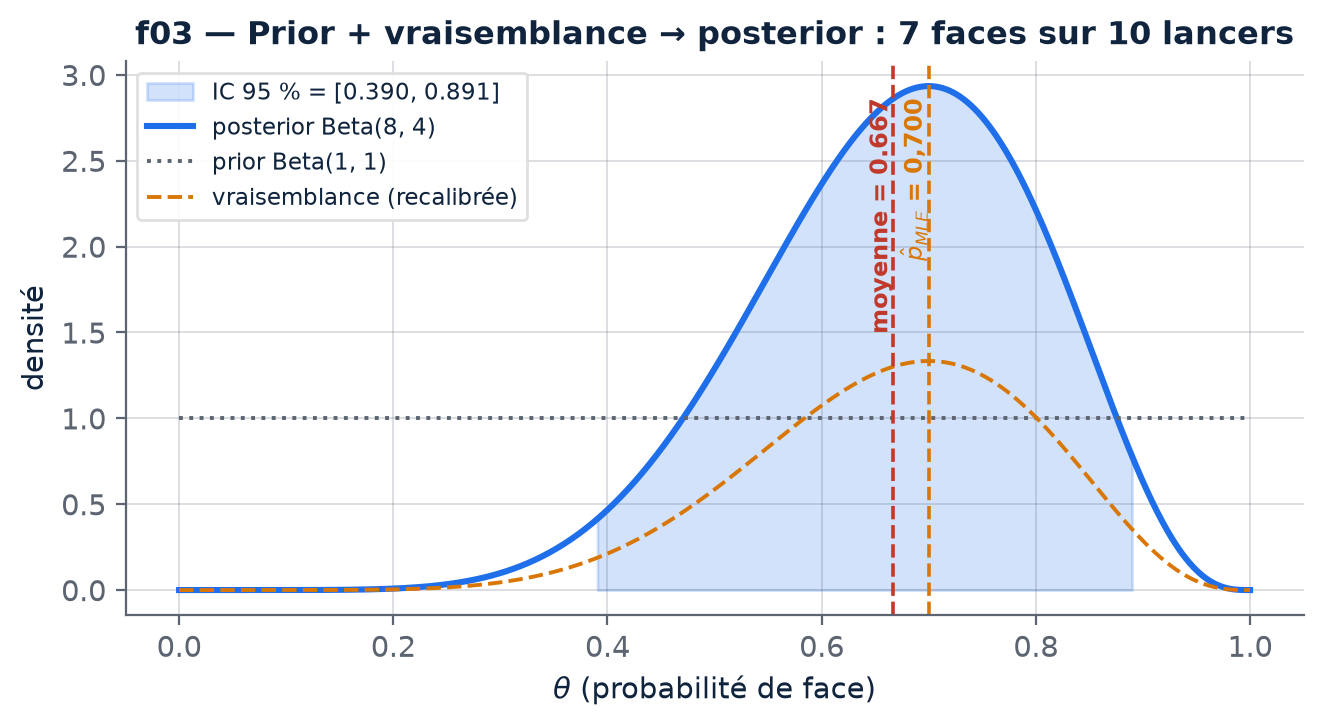
\includegraphics[width=.86\textwidth]{f03_piece_posterior.png}
\end{center}
\end{frame}

% [split]
\begin{frame}{Exemple fondateur : la pièce truquée --- le posterior}

\vspace{-1mm}
\begin{solbox}[Résultats calculés (script \file{src/fig\_ch1.py}, exécuté)]
\centering\small
posterior $\mathrm{Beta}(8,4)$ \quad|\quad moyenne $0{,}667$ \quad|\quad mode $0{,}700$
\quad|\quad IC 95 \% $[0{,}390 \,;\, 0{,}891]$ \quad|\quad $P(\theta > 0{,}5 \given y) = 0{,}887$
\end{solbox}
\end{frame}

% ---------------------------------------------------------------- 15
% [suite]
\begin{frame}{Comment lire un résultat bayésien}
\begin{columns}[t]
\begin{column}{0.5\textwidth}
\begin{kbox}[Trois nombres]
\begin{itemize}
  \item \textbf{Moyenne a posteriori} $0{,}667$ : minimise l'erreur quadratique,
        c'est l'estimateur par défaut.
  \item \textbf{Médiane} : robuste, sert au calcul du HDI.
  \item \textbf{Mode (MAP)} $0{,}700$ : coïncide ici avec le maximum de vraisemblance.
        Avec un prior asymétrique, il s'en écarte — c'est le \emph{shrinkage}.
\end{itemize}
\end{kbox}
\end{column}
\begin{column}{0.47\textwidth}
\begin{solbox}[Intervalle de crédibilité 95 \%]
$[0{,}390 \,;\, 0{,}891]$

\vspace{1.5mm}
\small « Il y a 95 \% de chance que la vraie probabilité de face soit dans cet intervalle,
\textbf{compte tenu du prior et des 7 faces observées}. »

\vspace{1.5mm}
Variante HDI (le plus court des intervalles de masse 0,95) : $[0{,}412 \,;\, 0{,}906]$ ---
légèrement plus court que l'intervalle à queues égales.
\end{solbox}
\end{column}
\end{columns}
\vspace{1mm}
\begin{ebox}[Effet mesurable du prior, mêmes données]
Avec $\theta \sim \mathrm{Beta}(2,2)$ au lieu de Beta$(1,1)$ : posterior $\mathrm{Beta}(9,5)$,
moyenne $0{,}643$, IC 95 \% $[0{,}386 \,;\, 0{,}861]$.
Le prior a ramené la croyance de 0,667 vers 0,643 : c'est le \textbf{\textit{shrinkage}}.
\end{ebox}
\vspace{1mm}
\end{frame}

% [suite]
\begin{frame}{Comment lire un résultat bayésien (suite)}
\begin{wbox}[À ne jamais écrire]
\nok{} « Il y a 95 \% de chance que la vraie valeur soit dans \emph{l'intervalle de confiance
fréquentiste} » \;; \;
\nok{} « $p(\theta) = 0{,}667$ est la probabilité que $\theta$ vaille exactement 0,667 »
(probabilité d'un point : nulle pour une loi continue).
\end{wbox}
\end{frame}

% ---------------------------------------------------------------- 16
\begin{frame}{Animation : mise à jour, observation après observation}
% [rogna]
\small
\begin{columns}[t]
\begin{column}{0.56\textwidth}
\begin{center}
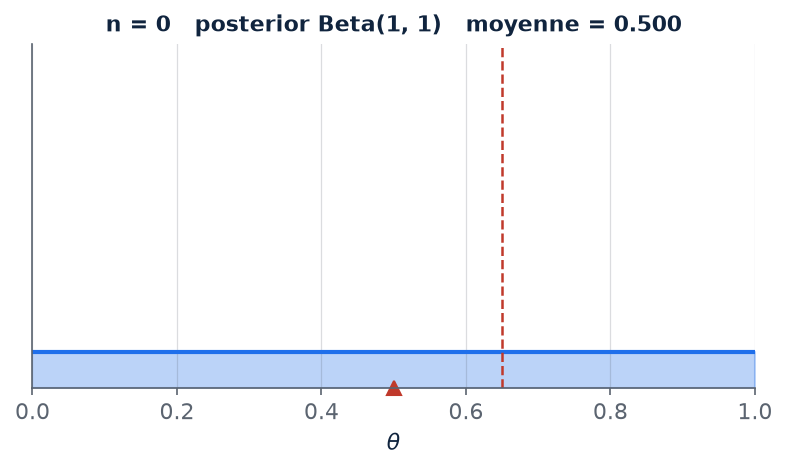
\includegraphics[width=\textwidth]{f04_frames/frame-0.png}
\end{center}
\vspace{-2mm}
\centering\footnotesize
\begin{tabular}{@{}llll@{}}
\toprule
$n$ & faces observées & posterior & moyenne \\
\midrule
0 (prior) & 0 & Beta$(1,1)$ & 0,500 \\
1 & 1 & Beta$(2,1)$ & 0,667 \\
5 & 5 & Beta$(6,1)$ & 0,857 \\
20 & 16 & Beta$(17,5)$ & 0,773 \\
200 & 121 & Beta$(122,80)$ & 0,604 \\
\bottomrule
\end{tabular}
\end{column}
\begin{column}{0.42\textwidth}
\begin{abox}[À faire devant la classe]
Ouvrir \file{notebooks/TP1\_mise\_a\_jour\_\allowbreak bayesienne.ipynb} et rejouer l'animation
($\alpha$, $\beta$ modifiables).

\vspace{1.5mm}
\textbf{Question :} à partir de quel $n$ une observation supplémentaire
déplace-t-elle la moyenne de moins de 0,005 ?
\end{abox}
\vspace{1mm}
\begin{ebox}[Réponse (calculée)]
Pour la réalisation simulée à $n = 200$, l'écart-type du posterior vaut $0{,}034$
et la moyenne ne bouge que de $\approx 0{,}002$ par nouvelle observation.
$5$ faces sur les $5$ premiers lancers donnaient 0,857 : \textbf{le petit échantillon
est extrême}, l'information ne s'achète pas, elle s'accumule en $1/\sqrt{n}$.
\end{ebox}
\end{column}
\end{columns}
\end{frame}

% ---------------------------------------------------------------- 17
% [split]
\begin{frame}{Application : sondage électoral}
\begin{center}
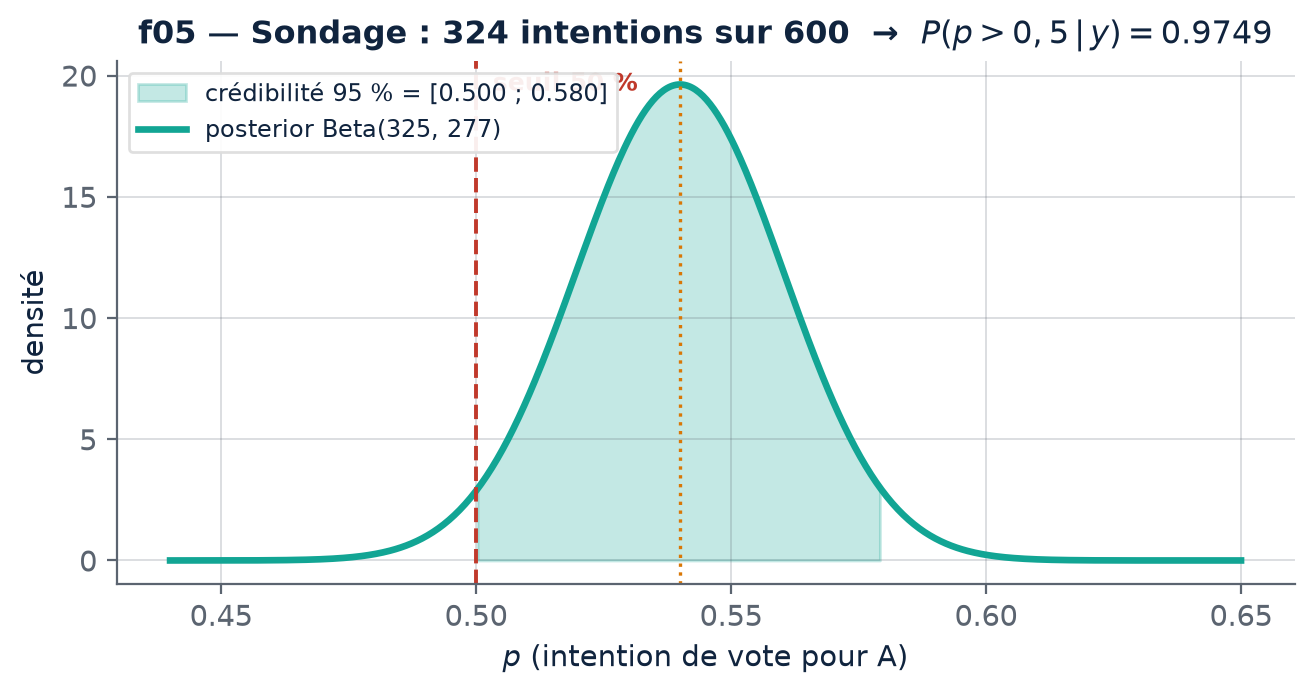
\includegraphics[width=\textwidth]{f05_sondage_posterior.png}
\end{center}
\end{frame}

% [split]
% [suite5]
\begin{frame}{Application : sondage électoral}
\begin{columns}[t]
\begin{column}{0.48\textwidth}
\begin{ebox}[Données]
$n = 600$ personnes interrogées, \textbf{324} intentions de vote pour A (54,0 \%).
Prior Beta$(1,1)$.
\end{ebox}
\begin{solbox}[Ce qu'on peut dire]
\begin{itemize}
  \item Posterior : $\mathrm{Beta}(325, 277)$, moyenne $0{,}540$
  \item Crédibilité 95 \% : $[0{,}500 \,;\, 0{,}580]$
  \item \textbf{$P(p > 0{,}5 \given y) = 0{,}975$}
  \item $P(p > 0{,}52) = 0{,}836$ \quad (intérêt : la marge d'un second tour)
  \item $P(p > 0{,}55) = 0{,}310$ \quad (le candidat est loin d'être certain de passer)
\end{itemize}
\end{solbox}
\end{column}
\end{columns}
\end{frame}

% [suite5]
\begin{frame}{Application : sondage électoral (suite)}
\begin{kbox}[L'avantage décisif]
Le fréquentiste donne $[0{,}50 \,;\, 0{,}58]$ mais ne peut pas répondre à
« le candidat A est-il \emph{probablement} au-dessus de 50 \% ? ».
Le bayésien répond : \textbf{97,5 \%}.
\end{kbox}
\end{frame}

% ---------------------------------------------------------------- 18
\begin{frame}{Pièges de lecture des intervalles}
\begin{columns}[t]
\begin{column}{0.49\textwidth}
\begin{wbox}[Intervalle de confiance fréquentiste]
\begin{itemize}
  \item Construit sur la variabilité de $\hat p$.
  \item \textbf{Ce dont on est sûr :} si l'on répétait l'étude un très grand nombre de fois,
        alors 95 \% des intervalles ainsi construits contiendraient $p$.
  \item \textbf{Ce dont on n'est pas sûr :} que \emph{cet} intervalle contienne $p$.
  \item Il ne peut pas devenir plus étroit quand on dispose d'information externe
        \emph{à moins} de changer la méthode.
\end{itemize}
\end{wbox}
\end{column}
\begin{column}{0.49\textwidth}
\begin{solbox}[Intervalle de crédibilité bayésien]
\begin{itemize}
  \item Construit sur la variabilité de $\theta$.
  \item \textbf{Ce dont on est sûr :} $P(\theta \in [a,b] \given y) = 0{,}95$.
  \item Il \textbf{rétrécit} mécaniquement si l'on ajoute de l'information externe
        justifiée (les priors conjugués du chapitre 2).
  \item Variante HDI : l'intervalle \emph{le plus court} de masse 0,95
        (chapitre 3, slide sur HDI contre queue égale).
\end{itemize}
\end{solbox}
\end{column}
\end{columns}
\vspace{1mm}
\centering\small
Les deux intervalles se ressemblent numériquement quand $n$ est grand —
ils \textbf{ne racontent pas la même chose}.
\end{frame}

% ---------------------------------------------------------------- 19
\begin{frame}{Le théorème de Bayes}
\begin{columns}[t]
\begin{column}{0.50\textwidth}
\begin{tcolorbox}[enhanced,colback=byDeep!6,colframe=byBlue,arc=2mm,
   boxrule=1pt,left=2mm,right=2mm,top=2mm,bottom=2mm]
\centering\large
\[
\underbrace{p(\theta \given y)}_{\text{a posteriori}}
\;=\;
\frac{\overbrace{p(y \given \theta)}^{\text{vraisemblance}}\;
      \overbrace{p(\theta)}^{\text{a priori}}}
     {\underbrace{\int p(y \given \theta')\,p(\theta')\,\mathrm{d}\theta'}_{\text{constante de normalisation}}}
\]
\end{tcolorbox}
\vspace{1mm}
\centering\small Forme proportionnelle, celle qu'on utilise en pratique :
\[\boxed{\;p(\theta \given y) \;\propto\; p(y \given \theta)\,p(\theta)\;}\]
\end{column}
\begin{column}{0.48\textwidth}
\begin{kbox}[Pourquoi c'est vrai]
Par définition de la probabilité conditionnelle :
\[
p(\theta \given y) = \frac{p(\theta, y)}{p(y)}
= \frac{p(y \given \theta)\,p(\theta)}{p(y)}
\]
et $p(y) = \int p(y \given \theta)p(\theta)\,\mathrm{d}\theta$
ne dépend \textbf{pas} de $\theta$.
\end{kbox}
\begin{wbox}[Le mot qui change tout]
L'intégrale du dénominateur est la \textbf{vraisemblance marginale}
$p(y)$ : c'est \emph{elle} qui décidera du facteur de Bayes et de la comparaison
de modèles (chapitre 4). Ici, on peut l'ignorer grâce à la proportionnalité.
\end{wbox}
\end{column}
\end{columns}
\end{frame}

% ---------------------------------------------------------------- 20
\begin{frame}{Démonstration pas à pas (3 lignes)}
\begin{abox}[On reprend la pièce truquée : prior Beta$(1,1)$, 7 faces sur 10]
\[
\begin{aligned}
\text{1. A priori}\quad & p(\theta) = \frac{\Gamma(2)}{\Gamma(1)\Gamma(1)}\theta^{0}(1-\theta)^{0} = 1 \\[1.5mm]
\text{2. Vraisemblance}\quad & p(y \given \theta) = \binom{10}{7}\theta^{7}(1-\theta)^{3} \\[1.5mm]
\text{3. Produit}\quad & p(\theta \given y) \propto \underbrace{\theta^{7}(1-\theta)^{3}}_{\text{le noyau seulement}}
\end{aligned}
\]
\end{abox}
\vspace{1mm}
\begin{solbox}[Reconnaître un noyau connu]
La forme $\theta^{7}(1-\theta)^{3}$ est le noyau d'une loi Beta de paramètres
$a-1 = 7$ et $b-1 = 3$, donc $a = 8$, $b = 4$ :
\[
p(\theta \given y) = \mathrm{Beta}(8,4) = \frac{\Gamma(12)}{\Gamma(8)\Gamma(4)}\theta^{7}(1-\theta)^{3}
\]
\textbf{La constante de normalisation n'a jamais eu besoin d'être calculée} : on l'a
retrouvée en reconnaissant le noyau. C'est le mécanisme de la conjugaison.
\end{solbox}
\end{frame}

% ---------------------------------------------------------------- 21
\begin{frame}{Bayes en quatre mots et en continu}
% [rogna]
\small
\begin{columns}[t]
\begin{column}{0.48\textwidth}
\begin{kbox}[Cas discret : la version de base]
\[
P(H \given E) = \frac{P(E \given H)\,P(H)}{P(E)}
\]
\begin{itemize}
  \item $H$ : hypothèse (malade, spam, modèle)
  \item $E$ : évidence (test positif, mot « gain »)
  \item $P(H)$ : croyance \emph{avant}
  \item $P(H \given E)$ : croyance \emph{après}
\end{itemize}
\end{kbox}
\begin{ebox}[Cotes, plus commode]
\[
\underbrace{\frac{P(H \given E)}{P(\bar H \given E)}}_{\text{cotes post.}}
=
\underbrace{\frac{P(H)}{P(\bar H)}}_{\text{cotes pri.}}
\times
\underbrace{\frac{P(E \given H)}{P(E \given \bar H)}}_{\text{rapport de vraisemblance}}
\]
Avec le spam : $0{,}25 \times 12 = 3 \Rightarrow P = 3/4 = 0{,}75$.
\end{ebox}
\end{column}
\begin{column}{0.48\textwidth}
\begin{ebox}[Cas continu : le paramètre]
\[
p(\theta \given y_1, \dots, y_n) \propto p(\theta)\prod_{i=1}^{n} p(y_i \given \theta)
\]
\begin{itemize}
  \item $\theta \in \R^d$ : paramètre (vecteur)
  \item $p(\theta)$ : densité a priori
  \item l'\textbf{i.i.d.} transforme le produit en somme de log
\end{itemize}
\end{ebox}
\begin{wbox}[Trois confusions classiques]
\begin{itemize}
  \item $p(\theta \given y) \neq p(y \given \theta)$ : les deux ne sont
        \textbf{pas} symétriques, la seconde est la vraisemblance.
  \item Une densité peut dépasser 1 : seule l'aire vaut 1.
  \item Le posterior \emph{dépend} du prior.
\end{itemize}
\end{wbox}
\end{column}
\end{columns}
\end{frame}

% ---------------------------------------------------------------- 22
\begin{frame}{Exercice guidé 1 --- détection de spam (10 min) --- l'énoncé}
\begin{ebox}[Énoncé]
Un filtre doit classer un courriel. On sait que :
\begin{itemize}
  \item 20 \% des courriels reçus sont des spams : $P(S) = 0{,}20$
  \item le mot « gain » apparaît dans 60 \% des spams : $P(G \given S) = 0{,}60$
  \item il apparaît dans 5 \% des courriels légitimes : $P(G \given \bar S) = 0{,}05$
\end{itemize}
\vspace{1.5mm}
\noindent\textbf{Question :} le mot « gain » est présent. Quelle est la probabilité
que ce courriel soit un spam ?
\end{ebox}
\vspace{1mm}
\begin{abox}[Question bonus (celle qui fait réfléchir)]
Et si « gain » apparaît \textbf{deux fois} ? \textbf{Quatre fois} ?
Quelle hypothèse êtes-vous obligé de faire ?
\end{abox}
\end{frame}

\begin{frame}{Exercice guidé 1 --- détection de spam}
\begin{center}
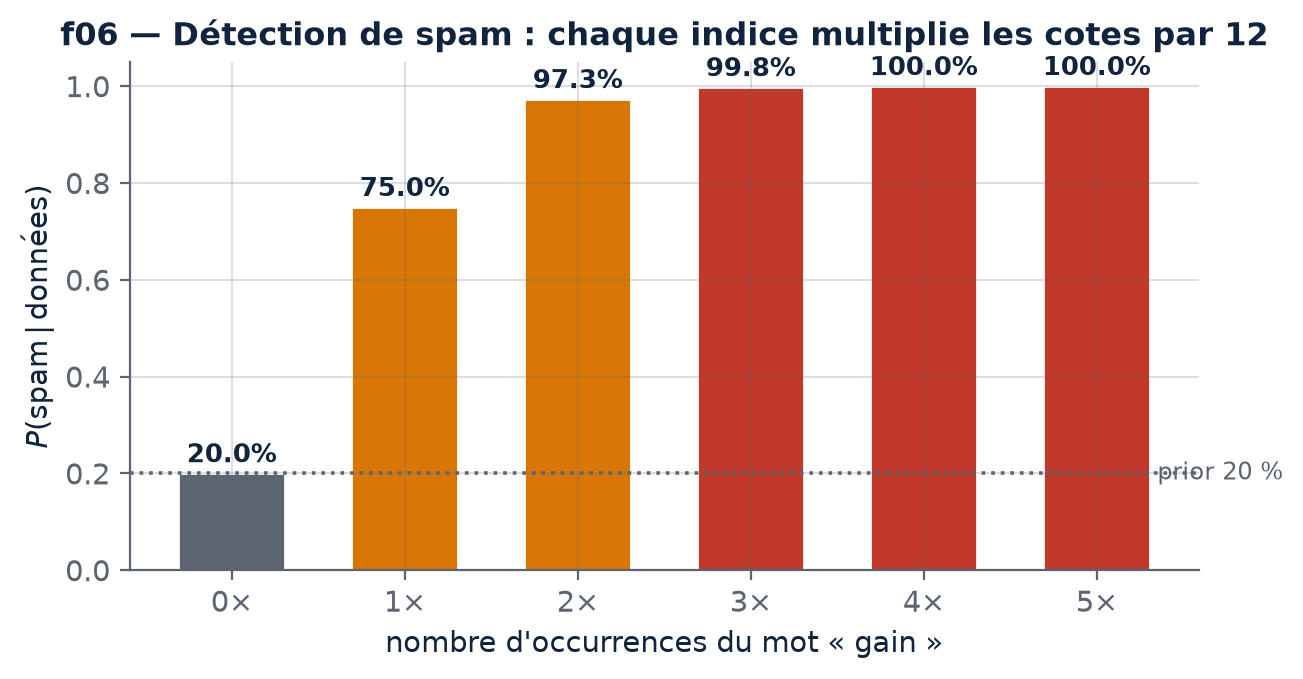
\includegraphics[width=.88\textwidth]{f06_spam.png}
\end{center}
\end{frame}

% ---------------------------------------------------------------- 23
\begin{frame}{Exercice guidé 1 — solution détaillée}
% [rogna]
\small
\begin{columns}[t]
\begin{column}{0.52\textwidth}
\begin{solbox}[Dénominateur d'abord]
\[
\begin{aligned}
P(G) &= P(G \given S)P(S) + P(G \given \bar S)P(\bar S)\\
     &= 0{,}60 \times 0{,}20 + 0{,}05 \times 0{,}80\\
     &= 0{,}12 + 0{,}04 = 0{,}16
\end{aligned}
\]
puis
\[
P(S \given G) = \frac{0{,}60 \times 0{,}20}{0{,}16} = 0{,}75
\]
Le score a été multiplié par 3 : les cotes passent de $1/4$ à $3/1$.
\end{solbox}
\end{column}
\begin{column}{0.46\textwidth}
\begin{ebox}[Occurrences répétées]
En supposant les occurrences \textbf{conditionnellement indépendantes} :
\[
P(S \given 2G) = \frac{0{,}60^2 \times 0{,}20}{0{,}60^2 \times 0{,}20 + 0{,}05^2 \times 0{,}80}
\]
\centering
\begin{tabular}{@{}lll@{}}
\toprule
Occurrences & Cotes & $P(S \given \cdot)$ \\
\midrule
0 & $0{,}25$ & 0,200 \\
1 & $3{,}0$ & \textbf{0,750} \\
2 & $36{,}0$ & \textbf{0,973} \\
3 & $432{,}0$ & \textbf{0,9977} \\
\bottomrule
\end{tabular}
\end{ebox}
\end{column}
\end{columns}
\vspace{1mm}
\begin{wbox}[Correction d'une erreur répandue]
On lit souvent « 2 occurrences $\Rightarrow$ 90 \% ». C'est faux : le calcul exact donne
\textbf{97,3 \%} ($0{,}25 \times 12^2 = 36$, soit $36/37$). Le facteur de Bayes se multiplie,
il ne s'additionne pas.
\end{wbox}
\end{frame}

% ---------------------------------------------------------------- 24
\begin{frame}{Quiz 2 — application directe}
\begin{qbox}[Question 2 -- Facteur 12]
Un filtre bayésien part d'un prior $P(S) = 0{,}20$ et traite chaque indice
indépendant comme un rapport de vraisemblance de 12.
\vspace{2mm}
Il faut dépasser 99 \% de certitude pour bloquer sans revue humaine.
Combien d'indices faut-il au minimum ?
\vspace{2mm}
\begin{enumerate}
  \item[(A)] 2 \quad \item[(B)] 3 \quad \item[(C)] 4 \quad \item[(D)] 6
\end{enumerate}
\vspace{2mm}
\textbf{Réponse : (B)} --- les cotes valent $0{,}25 \times 12^k$ ;
$k = 3$ donne 432, soit $0{,}9977 > 0{,}99$. Avec $k = 2$ on plafonne à 0,973.
\end{qbox}
\vspace{1.5mm}
\begin{kbox}[Ce que ce petit calcul enseigne]
La \textbf{mise à jour séquentielle} est une addition de log-cotes :
$\log(\text{cotes post.}) = \log(\text{cotes pri.}) + \sum_k \log(\text{LR}_k)$.
C'est exactement l'architecture d'un Naive Bayes, et c'est la raison pour laquelle
il tient sur un téléphone.
\end{kbox}
\end{frame}

% ---------------------------------------------------------------- 25
\begin{frame}{Exercice guidé 2 — le test COVID (10 min)}
\begin{columns}[t]
\begin{column}{0.47\textwidth}
\begin{ebox}[Énoncé]
Un test antigénique a
\begin{itemize}
  \item sensibilité $P(T^+ \given M) = 0{,}95$
  \item spécificité $P(T^- \given \bar M) = 0{,}98$
\end{itemize}
On teste une personne tirée au hasard dans une population où la prévalence est
de \textbf{5 \%}.
\vspace{1.5mm}
\textbf{Question :} le test est positif.
Quelle est la probabilité qu'elle soit réellement malade ?
\vspace{1.5mm}

\noindent\textcolor{byBlue}{\textbf{Indice :}} commencez par compter sur 1000 personnes.
\end{ebox}
\end{column}
\begin{column}{0.51\textwidth}
\begin{solbox}[Résolution en arbre]
Sur 1000 personnes :
\begin{itemize}
  \item 50 malades : $50 \times 0{,}95 = 47{,}5$ positifs
  \item 950 saines : $950 \times 0{,}02 = 19$ faux positifs
\end{itemize}
\[
P(M \given T^+) = \frac{47{,}5}{47{,}5 + 19} = \frac{47{,}5}{66{,}5} = \mathbf{0{,}714}
\]
\centering\footnotesize
Même sensibilité, même spécificité : la réponse dépend entièrement du contexte.
\end{solbox}
\end{column}
\end{columns}
\end{frame}

% ---------------------------------------------------------------- 26
% [split]
\begin{frame}{Le même test, six vérités différentes}
\begin{center}
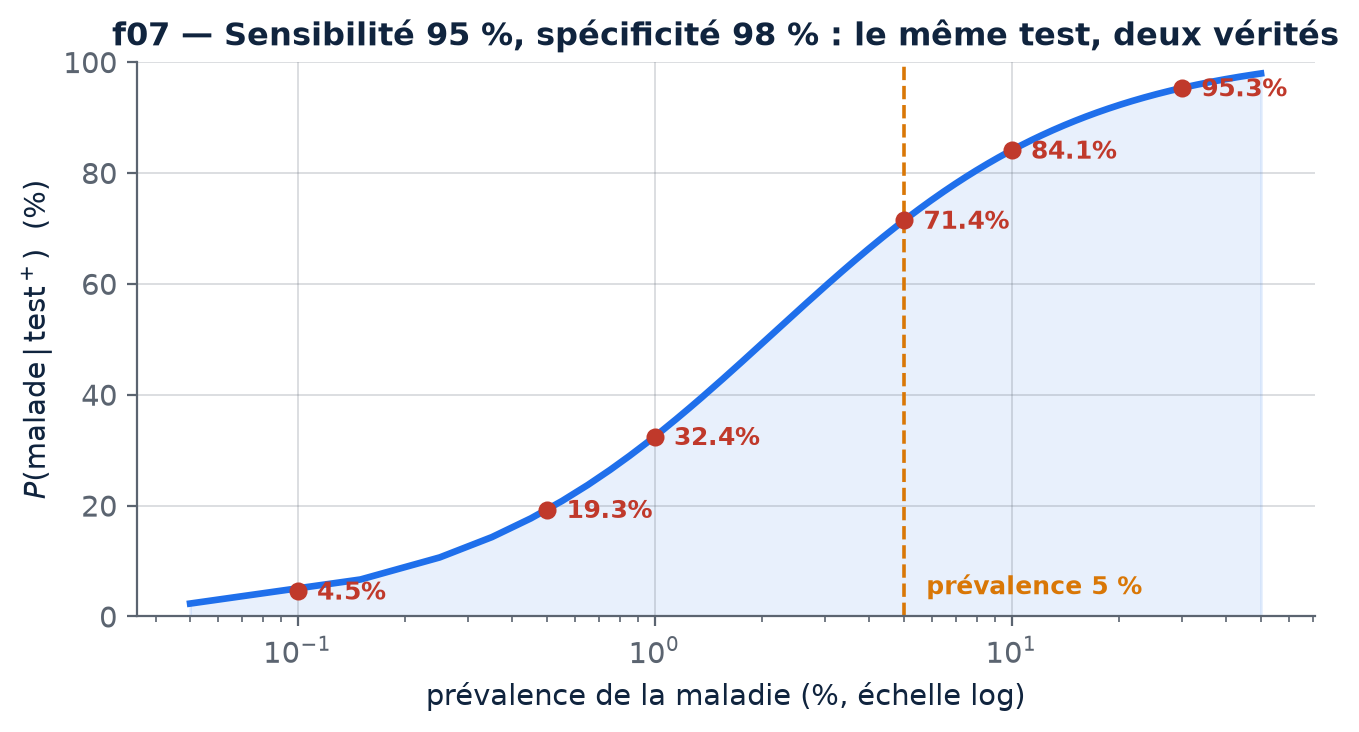
\includegraphics[width=.86\textwidth]{f07_covid_ppv.png}
\end{center}
\end{frame}

% [split]
\begin{frame}{Le même test, six vérités différentes}

\vspace{-1mm}
\begin{columns}[t]
\begin{column}{0.62\textwidth}
\begin{tabular}{@{}lcccccc@{}}
\toprule
Prévalence & 0,1 \% & 0,5 \% & 1 \% & 5 \% & 10 \% & 30 \% \\
\midrule
$P(M \given T^+)$ & 4,5 \% & 19,3 \% & 32,4 \% & \textbf{71,4 \%} & 84,1 \% & 95,3 \% \\
\bottomrule
\end{tabular}
\vspace{1.5mm}

\small Toutes ces valeurs sortent du calcul exécuté dans \file{src/fig\_ch1.py}.
\end{column}
\begin{column}{0.36\textwidth}
\begin{kbox}[Le cœur du cours]
La prévalence \textbf{est} un prior. La formule de Bayes n'est pas une recette de
calcul : c'est la déclaration explicite qu'\emph{une conclusion dépend de ce qu'on
croyait avant de mesurer}.
\end{kbox}
\end{column}
\end{columns}
\end{frame}

% ---------------------------------------------------------------- 27
% [suite5]
\begin{frame}[fragile]{Boîte à outils : la fonction qui fait tout}
% [rogna]
\small
\begin{columns}[t]
\begin{column}{0.53\textwidth}
\begin{codebox}[bayes.py — version minimale et générale]
\begin{lstlisting}
import numpy as np
from scipy import stats

def posterior_discret(prior_grid, prior_pdf, vraisemblance, y):
    """Posterior sur une grille : suffit des que theta est
    de dimension 1 ou 2. Aucune formule close requise."""
    post = prior_pdf(prior_grid) * vraisemblance(prior_grid, y)
    post /= np.trapezoid(post, prior_grid)     # normalisation
    return post

def proba(prior_grid, post, seuil):
    """P(theta > seuil | y) : LA question a laquelle le
    frequentiste ne peut pas repondre."""
    m = prior_grid > seuil
    return np.trapezoid(post[m], prior_grid[m])

def intervale_credibilite(prior_grid, post, niveau=0.95):
    c = np.cumsum(post) / post.sum()
    lo = prior_grid[np.searchsorted(c, (1 - niveau) / 2)]
    hi = prior_grid[np.searchsorted(c, 1 - (1 - niveau) / 2)]
    return lo, hi
\end{lstlisting}
\end{codebox}
\end{column}
\begin{column}{0.45\textwidth}
\begin{kbox}[Trois fonctions, tout le chapitre]
\begin{itemize}
  \item \textbf{grille $+$ normalisation} : la méthode universelle quand
        aucune conjugaison n'est disponible ;
  \item \textbf{proba dépassant un seuil} : la question décisionnelle ;
  \item \textbf{intervalle de crédibilité} : la synthèse de l'incertitude.
\end{itemize}
\end{kbox}
\end{column}
\end{columns}
\end{frame}

% [suite5]
\begin{frame}{Boîte à outils : la fonction qui fait tout (suite)}
\begin{wbox}[Quand la grille ne suffit plus]
En dimension $d$, une grille coûte $n^d$ points : impossible au-delà de
$d \approx 3$. C'est \textbf{exactement} le mur qui a motivé les méthodes MCMC
(chapitre 5).
\end{wbox}
\end{frame}

% ---------------------------------------------------------------- 28
\begin{frame}{Ce qui change quand le paramètre devient continu}
\begin{columns}[t]
\begin{column}{0.49\textwidth}
\begin{ebox}[Cas continu, exemple complet]
Mesures répétées d'une grandeur physique, $y_i \sim \N(\mu, \sigma^2)$ avec
$\sigma$ connu :
\[
\begin{aligned}
p(\mu) &= \N(\mu_0, \tau_0^2) \quad\text{(prior)}\\
p(y \given \mu) &\propto \prod_{i=1}^n e^{-\frac{(y_i-\mu)^2}{2\sigma^2}}\\
&\propto e^{-\frac{n(\bar y - \mu)^2}{2\sigma^2}}
\end{aligned}
\]
Le posterior est encore \textbf{normal} : $\N(\mu_n, \tau_n^2)$ avec
\[
\frac{1}{\tau_n^2} = \frac{1}{\tau_0^2} + \frac{n}{\sigma^2}
\]
\end{ebox}
\end{column}
\begin{column}{0.49\textwidth}
\begin{kbox}[Lecture : la précision s'additionne]
Ce n'est pas $\mu$ qui s'additionne, c'est l'\textbf{information}
$1/$variance. Le posterior est la moyenne pondérée des deux sources,
avec les poids $1/\tau_0^2$ et $n/\sigma^2$.
\vspace{1mm}
\[
\mu_n = \frac{\frac{\mu_0}{\tau_0^2}+\frac{n\bar y}{\sigma^2}}{\frac{1}{\tau_0^2}+\frac{n}{\sigma^2}}
\]
\end{kbox}
\begin{ebox}[Chiffres]
Avec $\mu_0 = 100$, $\tau_0 = 10$, $\sigma = 5$, $n = 4$, $\bar y = 92$ :
$\mu_n = 93{,}3$ et $\tau_n = 2{,}44$.
Le prior pèse encore, mais les données dominent déjà.
\end{ebox}
\end{column}
\end{columns}
\end{frame}

% ---------------------------------------------------------------- 29
% [suite]
% [suite5]
\begin{frame}{La constante de normalisation : pourquoi on l'ignore}
\begin{columns}[t]
\begin{column}{0.52\textwidth}
\begin{kbox}[Le raisonnement]
\[
p(\theta \given y) = \frac{p(y \given \theta)p(\theta)}{\underbrace{p(y)}_{\text{indépendant de }\theta}}
\]
$p(y)$ est le \emph{même nombre} pour toutes les valeurs de $\theta$ :
il \textbf{recentre} la courbe, il ne la \textbf{redessine} pas. Pour
comparer deux valeurs de $\theta$, il disparaît.
\end{kbox}
\end{column}

\begin{column}{0.46\textwidth}
\begin{wbox}[Ne l'oubliez jamais : il revient]
$p(y)$ réapparaît dans trois situations \textbf{décisives} :
\begin{itemize}
  \item \textbf{Comparer deux modèles} : c'est le facteur de Bayes
        $BF_{12} = p(y \given M_1)/p(y \given M_2)$ (chapitre 4) ;
  \item \textbf{Choisir un prior} : $p(y)$ mesure la \emph{plausibilité}
        du prior avant de voir les données (checks prédictifs a priori) ;
  \item \textbf{Modèles hiérarchiques} : il faut intégrer les effets
        latents pour évaluer la vraisemblance marginale.
\end{itemize}
\end{wbox}
\end{column}
\end{columns}
\end{frame}

% [suite5]
\begin{frame}{La constante de normalisation : pourquoi on l'ignore (suite)}
\begin{ebox}[Ordre de grandeur]
Dans l'exemple Beta-Binomial, $p(y)$ vaut exactement
$P(Y = 7)$ sous la loi prédictive a priori :
\[
p(y) = \binom{10}{7}\frac{\Gamma(2)\Gamma(11)}{\Gamma(13)} = \frac{1}{12} = 0{,}0833
\]
Le posterior $\mathrm{Beta}(8,4)$ divisé par ce facteur redonne bien une densité d'aire 1.
\end{ebox}
\end{frame}

% [suite]
\begin{frame}{La constante de normalisation : pourquoi on l'ignore (suite)}
\begin{kbox}[Règle pratique]
On travaille en \textbf{logarithme} :
$\log p(\theta \given y) = \log p(y \given \theta) + \log p(\theta) + \text{cte}$.
Toute l'inférence numérique (grilles, MCMC, VI) optimise ou échantillonne ce log-posterior.
\end{kbox}

\end{frame}

% ---------------------------------------------------------------- 30
\begin{frame}{Le mécanisme : une multiplication, pas une recette}
\begin{center}
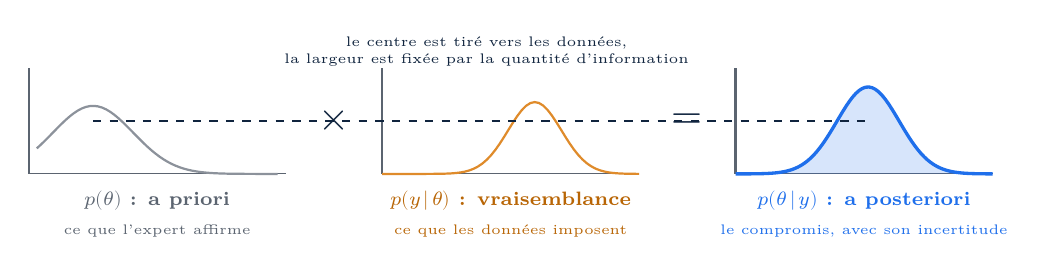
\begin{tikzpicture}[xscale=1.02,yscale=.96]
% --- prior
\draw[byGrey,thin] (-0.1,0) -- (3.1,0);
\draw[-,thick,byGrey] (-0.1,0) -- (-0.1,1.4);
\draw[byGrey!70,thick,domain=0:3,samples=60] plot (\x,{0.9*exp(-((\x-0.7)^2)/0.5)});
\node[byGrey,font=\scriptsize\bfseries] at (1.5,-0.35) {$p(\theta)$ : a priori};
\node[byGrey,font=\tiny] at (1.5,-0.75) {ce que l'expert affirme};
% --- x
\node[byDeep,font=\Large\bfseries] at (3.7,0.7) {$\times$};
% --- vraisemblance
\draw[byGrey,thin] (4.3,0) -- (7.5,0);
\draw[-,thick,byGrey] (4.3,0) -- (4.3,1.4);
\draw[byOrange!85,thick,domain=4.3:7.5,samples=60]
   plot (\x,{0.95*exp(-((\x-6.2)^2)/0.22)});
\node[byOrange!85!black,font=\scriptsize\bfseries] at (5.9,-0.35) {$p(y \given \theta)$ : vraisemblance};
\node[byOrange!85!black,font=\tiny] at (5.9,-0.75) {ce que les données imposent};
% --- =
\node[byDeep,font=\Large\bfseries] at (8.1,0.7) {$=$};
% --- posterior
\draw[byGrey,thin] (8.7,0) -- (11.9,0);
\draw[-,thick,byGrey] (8.7,0) -- (8.7,1.4);
\draw[byBlue,very thick,domain=8.7:11.9,samples=80]
   plot (\x,{1.15*exp(-((\x-10.35)^2)/0.30)});
\fill[byBlue,opacity=.18,domain=8.7:11.9,samples=80]
   (8.7,0) -- plot (\x,{1.15*exp(-((\x-10.35)^2)/0.30)}) -- (11.9,0) -- cycle;
\node[byBlue,font=\scriptsize\bfseries] at (10.3,-0.35) {$p(\theta \given y)$ : a posteriori};
\node[byBlue,font=\tiny] at (10.3,-0.75) {le compromis, avec son incertitude};
% --- annotations
\draw[byDeep,dashed,thin] (0.7,0.7) -- (10.35,0.7);
\node[byDeep,font=\tiny,align=center] at (5.6,1.62) {le centre est tiré vers les données, \\ la largeur est fixée par la quantité d'information};
\end{tikzpicture}
\end{center}
\vspace{1mm}
\begin{columns}[t]
\begin{column}{0.48\textwidth}
\begin{kbox}[Trois cas]
\begin{itemize}
  \item $\,$ prior étroit, données rares $\Rightarrow$ le prior gagne ;
  \item prior large, données nombreuses $\Rightarrow$ les données gagnent ;
  \item les deux étroits et \textbf{déplacés} $\Rightarrow$ conflit prior/données :
        \textbf{signalez-le}, ne le cachez pas.
\end{itemize}
\end{kbox}
\end{column}
\begin{column}{0.48\textwidth}
\begin{abox}[Démonstration en direct]
On rejoue la même figure avec $\alpha,\beta$ modifiables et
$n$ croissant dans le notebook
\file{TP1\_mise\_a\_jour\_\allowbreak bayesienne.ipynb} (dossier \file{notebooks/}), section 4.
\end{abox}
\end{column}
\end{columns}
\end{frame}

% ---------------------------------------------------------------- 31
\begin{frame}{Mise à jour séquentielle : la version formelle}
\begin{columns}[t]
\begin{column}{0.5\textwidth}
\begin{kbox}[Traitement par lot]
\[
p(\theta \given y_1,\dots,y_n) \propto p(\theta)\prod_{i=1}^{n}p(y_i \given \theta)
\]
\end{kbox}
\begin{kbox}[Traitement en flux (= c'est pareil)]
\[
\begin{aligned}
p(\theta \given y_1) &\propto p(\theta)\,p(y_1 \given \theta)\\
p(\theta \given y_1,y_2) &\propto p(\theta \given y_1)\,p(y_2 \given \theta)\\
&\;\;\vdots
\end{aligned}
\]
Aucune information n'est perdue : le posterior contient
\emph{toute} l'information apportée par les données déjà vues.
\end{kbox}
\end{column}
\begin{column}{0.48\textwidth}
\begin{ebox}[Conséquence majeure]
Un modèle bayésien peut être \textbf{actualisé en continu} : c'est ce qui
rend le filtrage de Kalman, les bandits bayésiens, l'arrêt anticipé des essais
cliniques et l'A/B testing séquentiel possibles \emph{sans pénalité de multiplicité}.
\end{ebox}
\begin{wbox}[Attention au raccourci]
« Le posterior suffit » n'est vrai que si le \textbf{modèle} est resté le même.
Changer de modèle (ajouter une covariable, abandonner la normalité) impose de
réévaluer le prior et la vraisemblance : le posterior d'un modèle A n'est
pas le prior d'un modèle B.
\end{wbox}
\end{column}
\end{columns}
\end{frame}

% ---------------------------------------------------------------- 32
\begin{frame}[fragile]{Exemple complet : régression linéaire bayésienne}
\begin{columns}[t]
\begin{column}{0.5\textwidth}
\begin{ebox}[Données et modèle]
12 mesures d'un rendement $y$ en fonction d'une dose $x$ (0 à 10).
\[
y_i = \beta_0 + \beta_1 x_i + \varepsilon_i, \qquad
\varepsilon_i \sim \N(0, \sigma^2)
\]
Priors \textbf{faiblement informatifs} :
\[
\beta_0 \sim \N(0, 5^2),\quad
\beta_1 \sim \N(0{,}5, 1^2),\quad
\sigma \sim \text{Demi-Normale}(2)
\]
\end{ebox}
\begin{kbox}[Pourquoi ces priors ?]
Volontairement larges : ils n'imposent rien de précis, mais ils
\textbf{empêchent des valeurs absurdes} (une pente de $10^6$). Ils disent
« je m'attends à un effet modéré, dans un ordre de grandeur raisonnable ».
\end{kbox}
\end{column}
\begin{column}{0.48\textwidth}
\begin{codebox}[PyMC — le modèle complet]
\begin{lstlisting}
with pm.Model() as modele:
    b0 = pm.Normal("b0", mu=0, sigma=5)
    b1 = pm.Normal("b1", mu=0.5, sigma=1)
    sigma = pm.HalfNormal("sigma", sigma=2)
    mu = b0 + b1 * x
    pm.Normal("y", mu=mu, sigma=sigma, observed=y)
    trace = pm.sample(draws=2000, tune=1500, chains=2)
\end{lstlisting}
\end{codebox}
\begin{abox}[Ce que l'on va lire sur le résultat]
\begin{itemize}
  \item la postérieure de chaque coefficient ;
  \item l'intervalle de crédibilité à 95 \% ;
  \item la prévision \textbf{avec} son incertitude.
\end{itemize}
\end{abox}
\end{column}
\end{columns}
\end{frame}

% ---------------------------------------------------------------- 33
% [rogna]
% [split]
\begin{frame}{Résultats réels (exécutés sur cette machine, CPU)}
\begin{center}
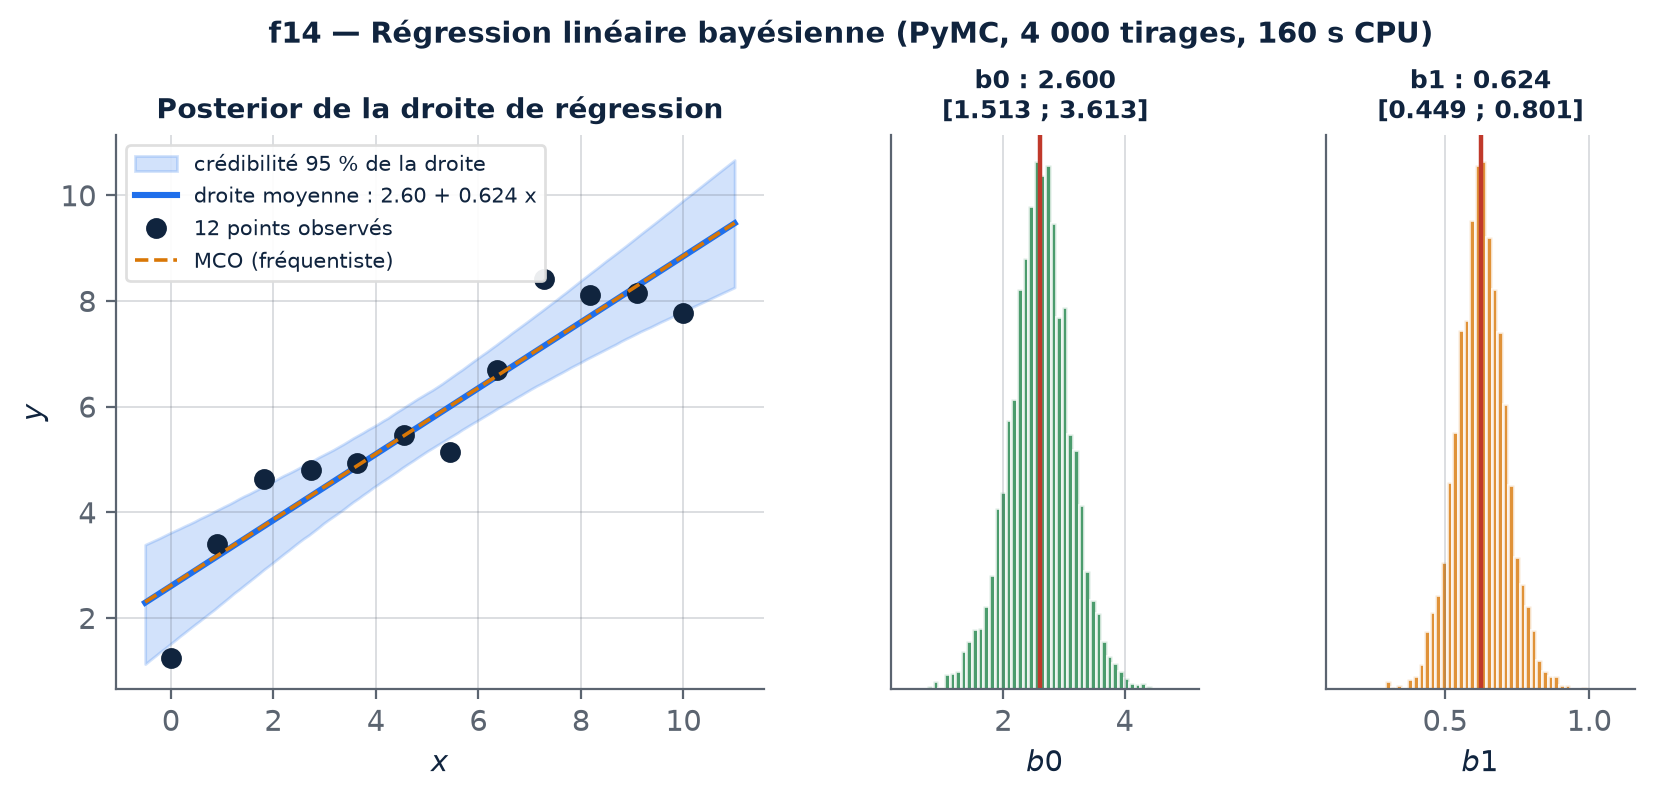
\includegraphics[width=.86\textwidth]{f14_regression_bayesienne.png}
\end{center}
\end{frame}

% [split]
\begin{frame}{Résultats réels (exécutés sur cette machine, CPU)}

\vspace{-1mm}
\begin{columns}[t]
\begin{column}{0.60\textwidth}
\begin{tabular}{@{}lccc@{}}
\toprule
Paramètre & Moyenne a post. & Crédibilité 95 \% & MCO (fréquentiste) \\
\midrule
$\beta_0$ (ordonnée) & 2,600 & $[1{,}513 \,;\, 3{,}613]$ & 2,611 \\
$\beta_1$ (pente) & 0,624 & $[0{,}449 \,;\, 0{,}801]$ & 0,624 \\
$\sigma$ (bruit) & 0,936 & --- & 0,92 \\
\bottomrule
\end{tabular}
\vspace{1mm}

\small Modèle échantillonné par NUTS : 2 chaînes, 4 000 tirages retenus,
$\hat R_{\max} = 1{,}0006$, 160 s sur un CPU 8 c\oe urs \emph{sans GPU}.
\end{column}
\begin{column}{0.38\textwidth}
\begin{kbox}[Apport du bayésien]
\begin{itemize}
  \item une \textbf{distribution} pour la pente, pas seulement un point ;
  \item $P(\beta_1 > 0 \given y) \approx 1$ : l'effet est certain ;
  \item avec 4 points au lieu de 12, MCO donnerait un IC énorme.

\end{itemize}
\end{kbox}
\end{column}
\end{columns}
\end{frame}

% ---------------------------------------------------------------- 34
% [split]
\begin{frame}{Prédire en bayésien : deux incertitudes, pas une}
\begin{center}
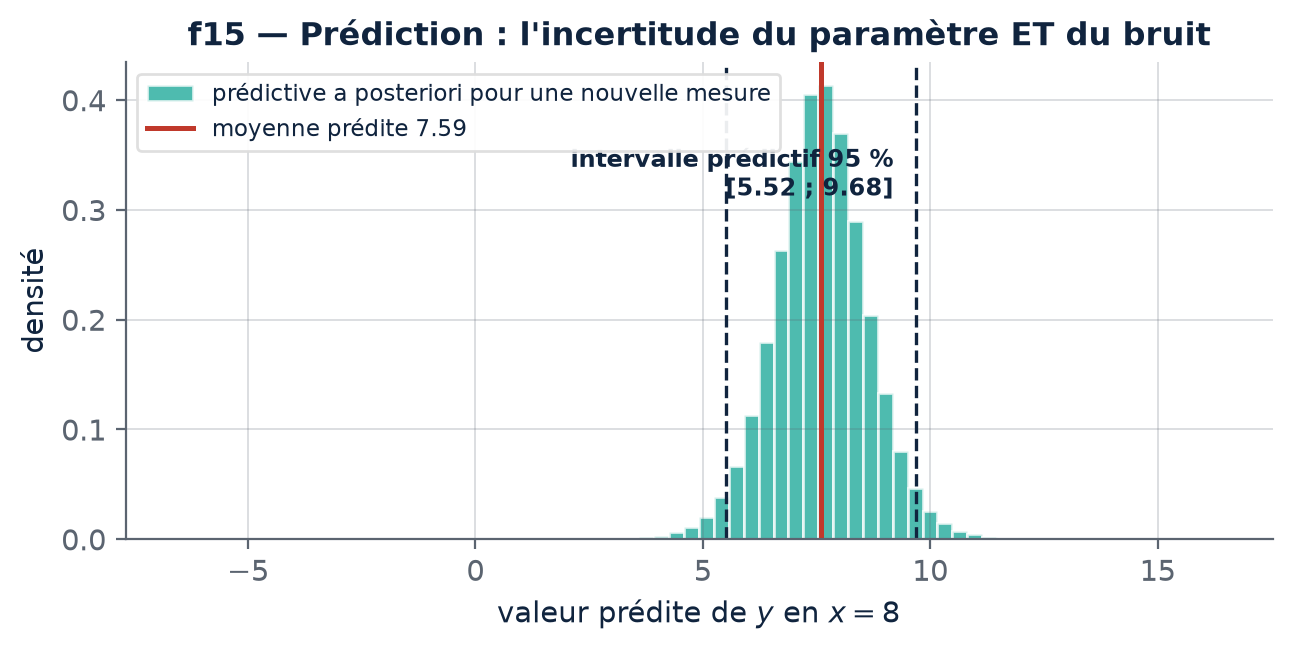
\includegraphics[width=\textwidth]{f15_prediction.png}
\end{center}
\end{frame}

% [split]
% [suite5]
\begin{frame}{Prédire en bayésien : deux incertitudes, pas une}
\begin{columns}[t]
\begin{column}{0.46\textwidth}
\begin{kbox}[La loi prédictive a posteriori]
\[
p(\tilde y \given y) = \int \underbrace{p(\tilde y \given \theta)}_{\text{bruit}}
\underbrace{p(\theta \given y)}_{\text{paramètre inconnu}} \mathrm{d}\theta
\]
On \textbf{intègre} sur l'incertitude du paramètre : la prédiction est
plus large qu'une prédiction faite à $\hat\theta$ fixé.
\end{kbox}
\begin{ebox}[Chiffres réels à $x = 8$]
\begin{itemize}
  \item valeur prédite moyenne : $7{,}59$
  \item crédibilité 95 \% de la \emph{moyenne} : $[6{,}83 \,;\, 8{,}40]$
  \item crédibilité 95 \% d'une \emph{observation} : $[5{,}52 \,;\, 9{,}68]$
\end{itemize}
\vspace{1mm}
\small L'écart entre les deux intervalles \textbf{est} la variabilité
$\sigma$ du processus : 0,94 ici.
\end{ebox}
\end{column}
\end{columns}
\end{frame}

% [suite5]
\begin{frame}{Prédire en bayésien : deux incertitudes, pas une (suite)}
\begin{wbox}[Erreur classique]
Confondre l'incertitude sur la \textbf{moyenne prédite} et celle sur la
\textbf{prochaine observation}. La seconde est toujours plus large et
c'est celle qui intéresse l'ingénieur.
\end{wbox}
\end{frame}

% ---------------------------------------------------------------- 35
\begin{frame}{Activité 2 — à vous de jouer (15 min)}
\begin{abox}[Consigne]
Par binôme, sur le jeu de données fourni \file{data/rendement\_12points.csv} (12 points,
colonnes \texttt{x} et \texttt{y}) :
\begin{enumerate}
  \item Refaites la régression de la slide précédente, mais avec un prior
        \textbf{très informatif} : $\beta_1 \sim \N(0{,}5, 0{,}05^2)$.
  \item Comparez la pente obtenue à celle du prior faiblement informatif.
  \item Que se passe-t-il si vous n'avez que les \textbf{4 premiers} points ?
        Le prior informatif aide-t-il ou trompe-t-il ?
  \item Rejouez l'analyse en doublant l'échelle de $x$ (convertissez $x$ en \% au lieu d'unités).
        Le prior sur $\beta_1$ devient-il raisonnable ?
\end{enumerate}
\end{abox}
\vspace{1mm}
\begin{columns}[t]
\begin{column}{0.48\textwidth}
\begin{kbox}[Ce que l'activité doit établir]
Un prior est \textbf{une hypothèse d'échelle}. Mal normalisé, il devient
une erreur silencieuse : le posterior sera précis et faux.
\end{kbox}
\end{column}
\begin{column}{0.48\textwidth}
\begin{kbox}[Indice]
Normaliser $x$ (centrer-réduire) rend les priors comparables entre études.
C'est la première recommandation pratique de Gelman.
\end{kbox}
\end{column}
\end{columns}
\end{frame}

% ---------------------------------------------------------------- 36
% [suite]
\begin{frame}{Correction collective et grille d'évaluation}
\begin{columns}[t]
\begin{column}{0.52\textwidth}
\begin{solbox}[Réponses attendues]
\begin{itemize}
  \item Prior $\N(0{,}5; 0{,}05^2)$ : le posterior de $\beta_1$ est
        \textbf{écrasé} autour de 0,5 (l'écart-type du prior est 10 fois trop petit).
  \item Avec 4 points seulement : le résultat suit le prior, l'intervalle de
        crédibilité est \emph{faussement étroit}. C'est le pire cas :
        \textbf{précis et faux}.
  \item En doublant l'échelle de $x$, la pente est divisée par 2 :
        le prior sur $\beta_1$ n'est plus adapté, il faut le renormaliser.
\end{itemize}
\end{solbox}
\end{column}
\begin{column}{0.46\textwidth}
{\setlength{\tabcolsep}{3pt}\begin{tabular}{@{}p{3.3cm}p{0.8cm}p{1.3cm}@{}}
\toprule
Critère d'évaluation & Points & Acquis ? \\
\midrule
Modèle PyMC correct et exécuté & 3 & \hspace{1.2cm} \\
Priors justifiés par écrit & 3 & \\
Comparaison chiffrée des deux priors & 3 & \\
Diagnostic de convergence ($\hat R$) & 2 & \\
Interprétation en une phrase & 3 & \\
Discussion de la sensibilité à l'échelle & 2 & \\
\midrule
\textbf{Total} & \textbf{16} & \\
\bottomrule
\end{tabular}}
\end{column}
\end{columns}
\vspace{1.5mm}
\end{frame}

% [suite]
\begin{frame}{Correction collective et grille d'évaluation (suite)}
\begin{wbox}[Le réflexe à acquérir]
Toujours se demander : \textbf{« mes données peuvent-elles seulement me contredire ? »}
Si non, votre prior est un dogme, pas un a priori.
\end{wbox}
\end{frame}

% ---------------------------------------------------------------- 37
\begin{frame}{Les deux écoles face au même jeu de données}
\begin{center}
\small
\begin{tabular}{@{}p{3.0cm}p{5.1cm}p{5.1cm}@{}}
\toprule
\textbf{Aspect} & \textbf{Fréquentiste} & \textbf{Bayésien} \\
\midrule
Ce qui est aléatoire & $\hat\theta$ (l'estimateur) sur des échantillons répétés
                     & $\theta$ (le paramètre) \\
Ce qui est fixe & $\theta$ & les données observées $y$ \\
Réponse donnée & point $+$ intervalle de confiance & distribution a posteriori \\
Question à laquelle on peut répondre & « si l'expérience était répétée \dots » &
« quelle est la plausibilité de ce que j'avance ? » \\
Information externe & non incorporable sans changer la méthode &
explicitée dans le prior \\
Arrêt anticipé & gonfle le risque de type I (sauf correction séquentielle) &
licite : la conclusion est conditionnelle aux données \\
Petits échantillons & inférence fragile, IC trompeur & le prior régularise
(\emph{shrinkage}) \\
Coût de calcul & faible (formules closes) & élevé (intégrales, MCMC) \\
Besoin de supervision & modèle seul & modèle \textbf{et} priors \\
\bottomrule
\end{tabular}
\end{center}
\vspace{1mm}
\begin{kbox}[La bonne posture]
Ce ne sont pas deux religions : ce sont deux façons de répondre à deux
\textbf{questions différentes}. Choisissez la question ; l'outil suivra.
\end{kbox}
\end{frame}

% ---------------------------------------------------------------- 38
% [rogna]
% [rogna]
% [rogna]
% [split]
\begin{frame}{La p-value n'est pas $P(H_0 \given \mathrm{données})$}
\begin{center}
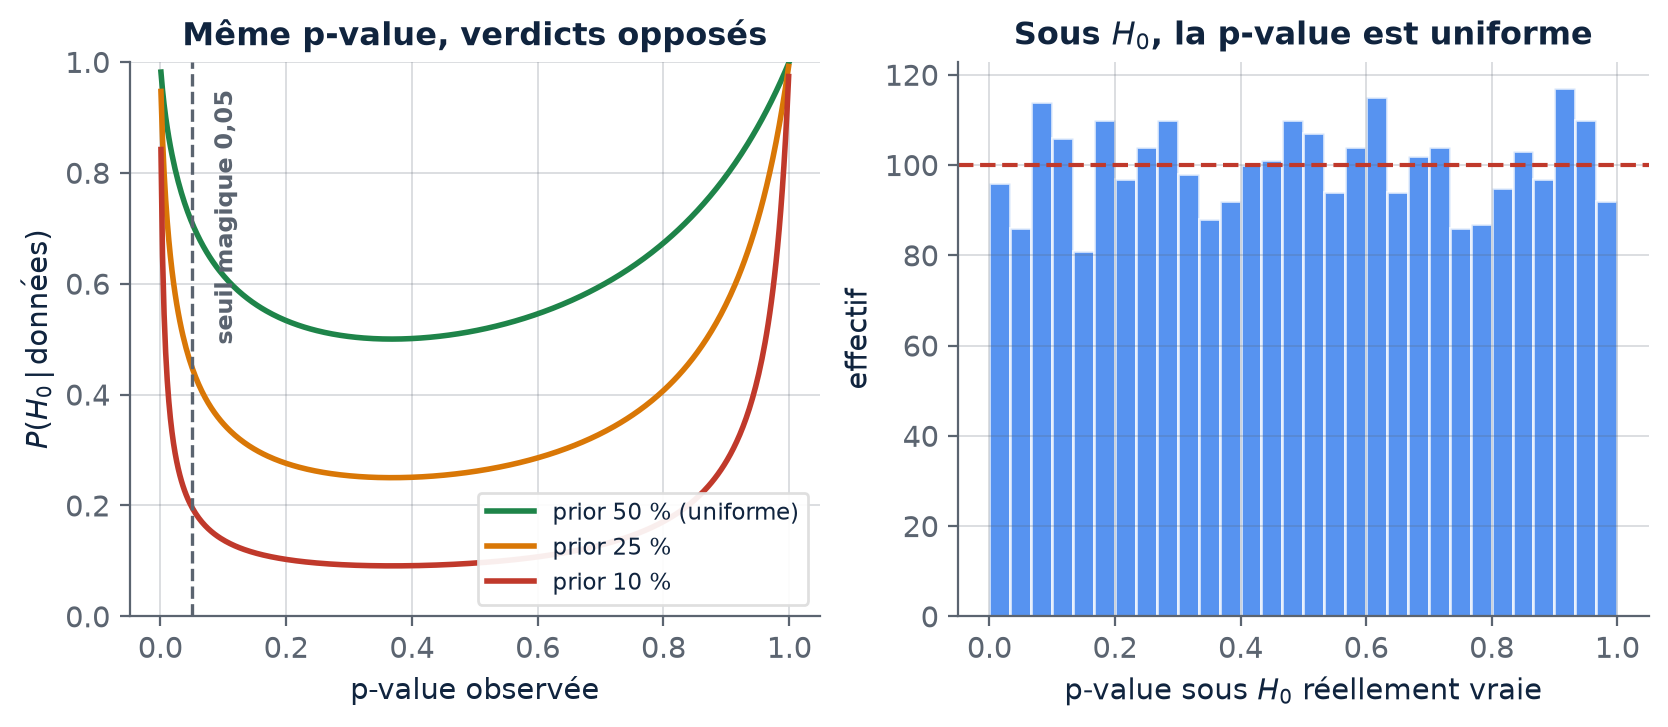
\includegraphics[width=.86\textwidth]{f08_pvalue_vs_posterior.png}
\end{center}
\end{frame}

% [split]
\begin{frame}{La p-value n'est pas $P(H_0 \given \mathrm{données})$}

\vspace{-1mm}
\begin{columns}[t]
\begin{column}{0.55\textwidth}
\begin{ebox}[Ce que la figure montre (calcul réel)]
Pour un test bilatéral, une p-value de $0{,}05$ \textbf{ne} signifie pas
« 5 \% de chance que $H_0$ soit vraie ». Avec un prior neutre
$P(H_0) = P(H_1) = 0{,}5$ et la calibration de Sellke--Johnson :
\[
BF_{01} \approx \frac{-1}{e\, p \log p} = 2{,}46
\;\Rightarrow\;
P(H_0 \given y) = 0{,}71
\]
\vspace{1mm}
\small Avec 10 \% de prior sur $H_0$ : $P(H_0 \given y) = 0{,}21$ ; avec 90 \% : $0{,}96$.
\textbf{Même p-value, trois conclusions.}
\end{ebox}
\end{column}
\begin{column}{0.43\textwidth}
\begin{kbox}[La formule à retenir]
$P(H_0 \given y)$ dépend de deux choses et de deux seulement :
\begin{itemize}
  \item ce que l'on croyait \textbf{avant} ($P(H_0)$) ;
  \item la force de l'évidence ($BF_{01}$).
\end{itemize}
La p-value ne contient que la seconde.
\end{kbox}
\end{column}
\end{columns}
\end{frame}

% ---------------------------------------------------------------- 39
% [suite]
\begin{frame}{Ce qu'une p-value dit — et ne dit pas}
\begin{columns}[t]
\begin{column}{0.48\textwidth}
\begin{solbox}[Ce qu'elle dit]
$p = P\big(T \text{ aussi extrême} \given H_0 \text{ vraie}\big)$

\vspace{1mm}
C'est une probabilité \textbf{des données}, conditionnelle à une hypothèse
que l'on n'a jamais testée directement. C'est une mesure de
\emph{surprise}, pas une mesure de \emph{preuve}.
\end{solbox}
\end{column}
\begin{column}{0.48\textwidth}
\begin{kbox}[La traduction bayésienne]
\[
\underbrace{\frac{P(H_0 \given y)}{P(H_1 \given y)}}_{\text{ce qui intéresse}}
=
\underbrace{\frac{P(H_0)}{P(H_1)}}_{\text{le contexte}}
\times
\underbrace{BF_{01}}_{\text{l'évidence}}
\]
Le bayésien rend explicites les deux facteurs que la p-value
\textbf{mélange} et cache.
\end{kbox}
\begin{ebox}[Chiffre à retenir de la simulation]
Sur 3 000 tests simulés avec $H_0$ \emph{réellement vraie}, la distribution
des p-values est \textbf{uniforme} : 5 \% des études afficheront $p < 0{,}05$
par pur hasard. Le seuil n'est pas une garantie.
\end{ebox}
\end{column}
\end{columns}
\end{frame}

% [suite]
\begin{frame}{Ce qu'une p-value dit — et ne dit pas (suite)}
\begin{wbox}[Ce qu'elle ne dit pas]
\begin{itemize}
  \item \nok{} $p = 0{,}03$ ne signifie pas « 3 \% de chance que $H_0$ soit vraie ».
  \item \nok{} $p > 0{,}05$ ne signifie pas « pas d'effet » : c'est
        « pas assez de données pour trancher ».
  \item \nok{} $p$ n'a pas d'interprétation \emph{après} avoir vu les données
        comme probabilité d'hypothèse.
  \item \nok{} $p$ dépend de l'intention d'arrêter l'expérience (arrêt séquentiel,
        tests multiples).
\end{itemize}
\end{wbox}
\end{frame}

% ---------------------------------------------------------------- 40
\begin{frame}{Sept avantages concrets du bayésien}
\begin{columns}[t]
\begin{column}{0.49\textwidth}
\begin{enumerate}
  \item \textbf{Réponse directe.} « $P(\theta > 0{,}5 \given y) = 0{,}975$ » :
        la question du décideur, sans traduction.
  \item \textbf{Information externe incorporée} explicitement et de façon
        auditable (prior, power prior, méta-analyse).
  \item \textbf{Petits échantillons maîtrisés} : le prior régularise
        (\emph{shrinkage}) au lieu de laisser exploser la variance.
  \item \textbf{Arrêt séquentiel licite} : la conclusion est conditionnelle aux
        données observées — un essai peut s'arrêter dès que la preuve est suffisante.
\end{enumerate}
\end{column}
\begin{column}{0.49\textwidth}
\begin{enumerate}
  \setcounter{enumi}{4}
  \item \textbf{Modèles hiérarchiques naturels} : les groupes échangent
        de l'information, indispensable pour les données groupées.
  \item \textbf{Propagation complète de l'incertitude} : la prédiction intègre
        l'incertitude des paramètres, des effets latents et du bruit.
  \item \textbf{Mise à jour continue} : le posterior d'aujourd'hui est le prior
        de demain, idéal pour un système en production.
\end{enumerate}
\vspace{1mm}
\begin{kbox}[Contrepartie honnête]
Aucun de ces avantages n'est gratuit : le prior doit être
\textbf{choisi, écrit et défendu}.
\end{kbox}
\end{column}
\end{columns}
\end{frame}

% ---------------------------------------------------------------- 41
\begin{frame}{Limites, coûts et objections légitimes}
\begin{columns}[t]
\begin{column}{0.48\textwidth}
\begin{wbox}[Les cinq coûts réels]
\begin{enumerate}
  \item \textbf{Calcul} : intégrales sans forme close $\Rightarrow$ MCMC.
        Notre régression à 3 paramètres : 160 s sur CPU ; un modèle hiérarchique
        réel demande des heures et un GPU.
  \item \textbf{Choix du prior} : impossible à automatiser, doit être justifié.
        Un prior vague n'est pas neutre, il est souvent pire qu'un prior réfléchi.
  \item \textbf{Diagnostic} : une chaîne qui n'a pas convergé produit des nombres
        \emph{faux mais crédibles}. Il faut apprendre à lire $\hat R$, ESS, trace.
  \item \textbf{Robustesse} : un prior mal calibré donne une réponse
        précise et erronée (slide 36).
  \item \textbf{Culture} : beaucoup de collègues, de revues et de jurys
        raisonnent encore en p-values.
\end{enumerate}
\end{wbox}
\end{column}
\begin{column}{0.48\textwidth}
\begin{kbox}[Objections fréquentes, réponses]
\textbf{« Le prior rend le résultat subjectif. »} \\
Tout modèle contient des choix subjectifs ; le bayésien est le seul à les
\emph{écrire}. Le test fréquentiste cache ses choix dans le plan d'analyse.

\vspace{1.5mm}
\textbf{« Avec beaucoup de données, le prior n'importe plus. »} \\
Vrai asymptotiquement (les données dominent en $n$), faux en pratique :
avec des données groupées ou peu nombreuses, le prior décide.

\vspace{1.5mm}
\textbf{« C'est trop lent pour la production. »} \\
Faux : la phase coûteuse est \emph{hors ligne} ; la prédiction en ligne
se fait par $\theta$ échantillonné, en microsecondes.
\end{kbox}
\end{column}
\end{columns}
\end{frame}

% ---------------------------------------------------------------- 42
\begin{frame}{Le détour par le fréquentiste : planifier une étude}
\begin{center}
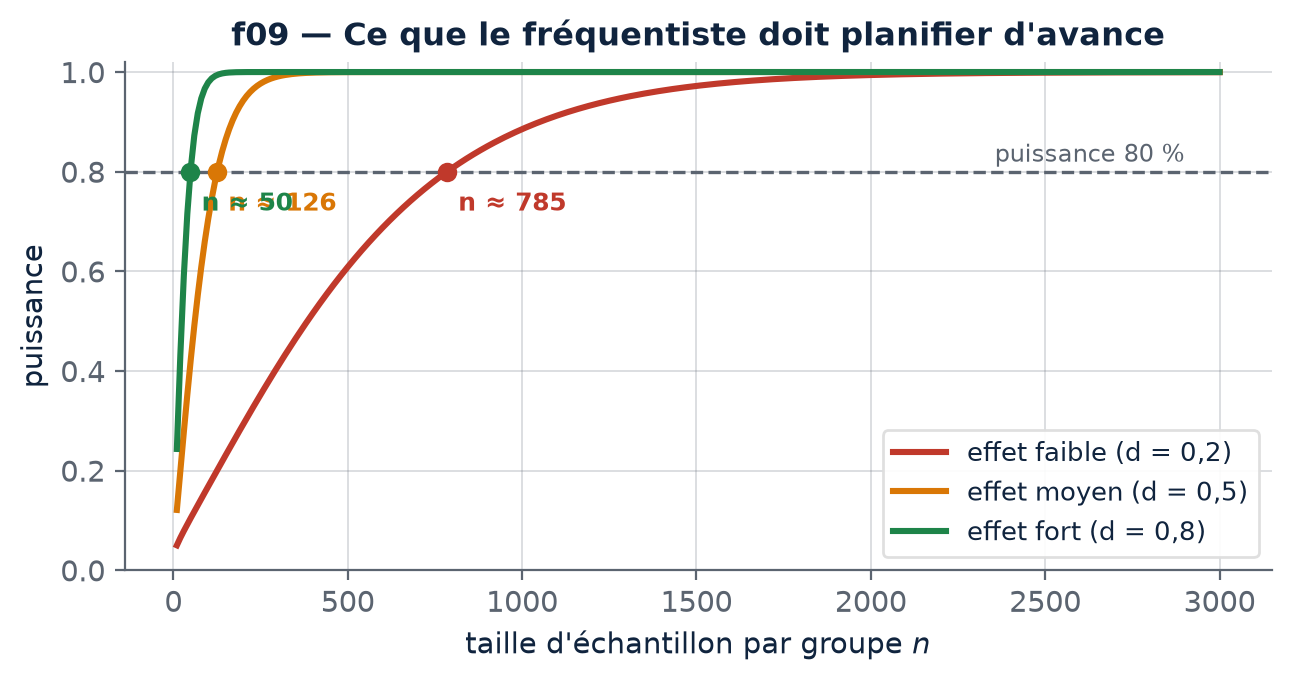
\includegraphics[width=0.58\textwidth]{f09_puissance.png}
\end{center}
\vspace{-1mm}
\begin{columns}[t]
\begin{column}{0.6\textwidth}
\begin{tabular}{@{}lccc@{}}
\toprule
Taille d'effet & $d = 0{,}2$ (faible) & $d = 0{,}5$ (moyen) & $d = 0{,}8$ (fort) \\
\midrule
$n$ par groupe pour 80 \% de puissance & 785 & 126 & 50 \\
\bottomrule
\end{tabular}
\vspace{1mm}

\small Calculé par la formule usuelle $n = 4(z_{1-\alpha/2}+z_{\text{puiss.}})^2/d^2$
(script \file{src/fig\_ch1.py}).
\end{column}
\begin{column}{0.38\textwidth}
\begin{kbox}[La réponse bayésienne]
Au lieu de fixer $n$ à l'avance, on suit
$P(\theta > \text{seuil} \given y_{1..n})$ et on arrête quand elle dépasse
un niveau fixé \textbf{avant} l'étude : la logique des essais adaptatifs.
\end{kbox}
\end{column}
\end{columns}
\end{frame}

% ---------------------------------------------------------------- 43
\begin{frame}{L'écosystème logiciel : quoi utiliser, quand}
% [rogna]
\footnotesize
\begin{center}
\footnotesize
{\setlength{\tabcolsep}{3pt}\begin{tabular}{@{}p{1.9cm}p{2.3cm}p{2.1cm}p{2.8cm}p{2.4cm}@{}}
\toprule
\textbf{Outil} & \textbf{Langage} & \textbf{Échantillonneur} & \textbf{Points forts} & \textbf{Quand le choisir} \\
\midrule
\textbf{PyMC} & Python & NUTS (PyTensor) & intégration NumPy/Pandas, ArviZ,
modèles hiérarchiques & \textbf{notre choix dans ce cours} \\
\textbf{Stan} & C++ $+$ R/Python & NUTS & référence en performance,
écosystème académique & modèles lourds, publication \\
\textbf{JAGS} & R & Gibbs & historique, très lisible & enseignement, modèles simples \\
\textbf{NumPyro} & Python & NUTS (JAX) & rapide, vectorisé, GPU & grands modèles, production \\
\textbf{ArviZ} & Python & --- & diagnostics et visualisation & avec PyMC ou NumPyro \\
\textbf{R} ($+$ \texttt{bayesplot}) & R & --- & graphiques prêts pour publication &
public cible R \\
\textbf{INLA} & R & Laplace déterministe & très rapide (GMRF) & champs gaussiens \\
\bottomrule
\end{tabular}}
\end{center}
\vspace{1mm}
\begin{kbox}[Le conseil du cours]
Un seul écosystème suffit pour tout apprendre : \textbf{Python $+$ PyMC $+$ ArviZ}.
Tout ce qui suit est exécutable sur un ordinateur portable sans GPU.
\end{kbox}
\end{frame}

% ---------------------------------------------------------------- 44
\begin{frame}[fragile]{Premier modèle complet — à taper et exécuter}
\begin{columns}[t]
\begin{column}{0.53\textwidth}
\begin{codebox}[premier\_modele.py]
\begin{lstlisting}
import pymc as pm
import arviz as az
import numpy as np

n, k = 10, 7

with pm.Model() as modele:
    theta = pm.Beta("theta", alpha=2, beta=2)      # prior
    pm.Binomial("y", n=n, p=theta, observed=k)     # vraisemblance

    # 1. echantillonnage a posteriori
    trace = pm.sample(draws=2000, tune=1000, chains=2)

    # 2. prediction pour 5 nouveaux lancers
    y_new = pm.Binomial("y_new", n=5, p=theta,
                        shape=5, observed=None)
    pred = pm.sample_posterior_predictive(trace)

print(az.summary(trace, hdi_prob=0.95))
print(pred.posterior_predictive["y_new"].mean())
\end{lstlisting}
\end{codebox}
\end{column}
\begin{column}{0.45\textwidth}
\begin{abox}[Lancez-le maintenant]
\begin{itemize}
  \item Sur cette machine (CPU, 2 chaînes, 3 000 itérations) :
        \textbf{5,8 secondes}.
  \item Vous venez d'estimer une distribution a posteriori complète
        sans écrire une seule intégrale.
\end{itemize}
\end{abox}
\begin{kbox}[Sortie attendue]
\begin{tabular}{@{}ll@{}}
postérieur moyen & $0{,}648$ \\
écart-type & $0{,}124$ \\
crédibilité 95 \% & $[0{,}383 \,;\, 0{,}864]$ \\
$\hat R$ & $1{,}0005$ \\
ESS & $1\,514$ \\
\end{tabular}
\vspace{1mm}

\footnotesize $1\,514$ tirages indépendants équivalents sur $4\,000$ : la chaîne
a une mémoire modérée, c'est acceptable.
\end{kbox}
\end{column}
\end{columns}
\end{frame}

% ---------------------------------------------------------------- 45
% [rogna]
% [rogna]
% [rogna]
\begin{frame}{Lire un résultat PyMC sans se tromper}
\begin{center}
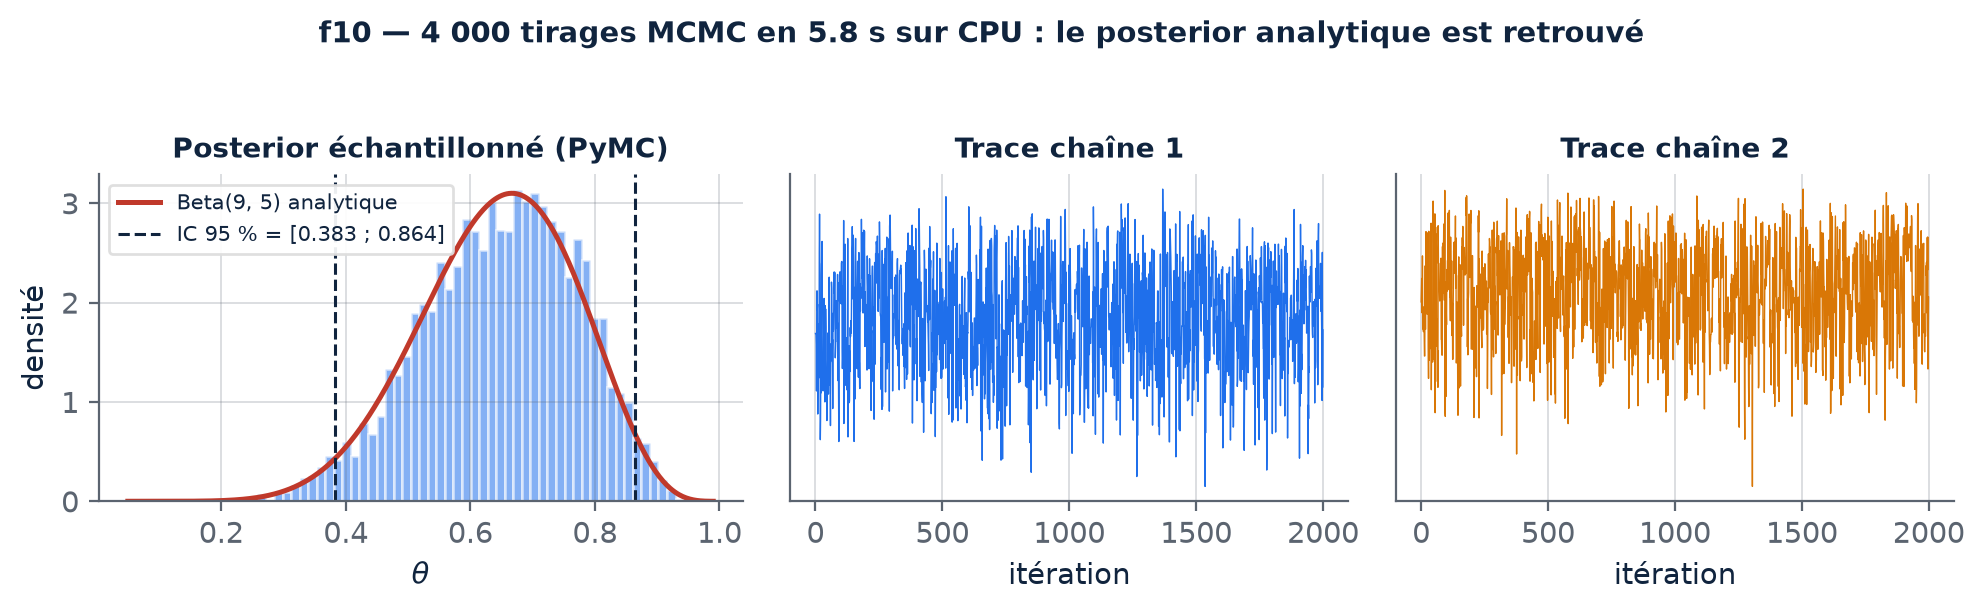
\includegraphics[width=.78\textwidth]{f10_pymc_coin.png}
\end{center}
\vspace{-1.5mm}
\begin{center}
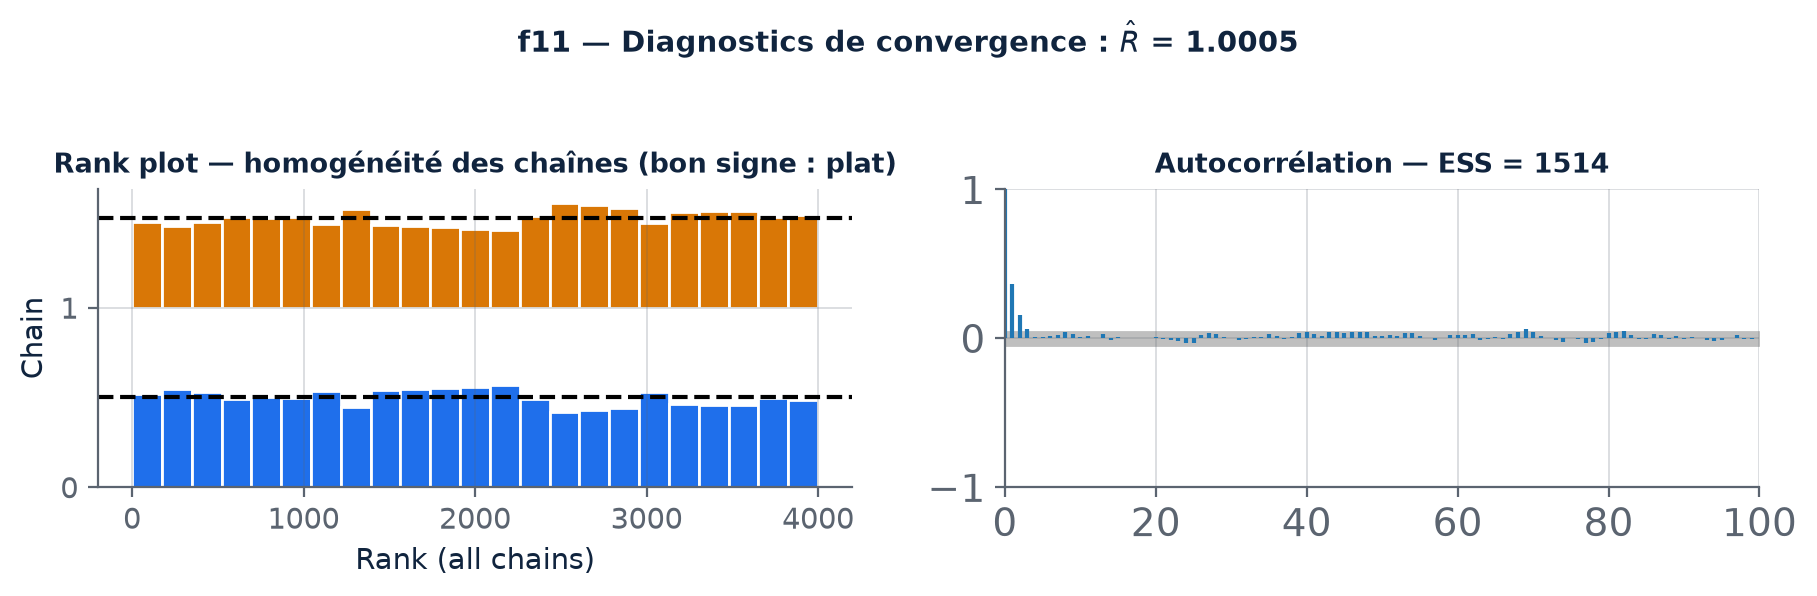
\includegraphics[width=.58\textwidth]{f11_pymc_diagnostics.png}
\end{center}
\vspace{-1mm}
\centering\small
L'histogramme des tirages MCMC reproduit la densité analytique $\mathrm{Beta}(9,5)$ (trait rouge) :
l'échantillonneur ne « fabrique » pas une réponse, il explore une densité.
Le \emph{rank plot} plat et l'autocorrélation qui retombe en quelques dizaines
d'itérations sont les deux signes d'une chaîne saine.
\end{frame}

% ---------------------------------------------------------------- 46
% [suite]
\begin{frame}{Les huit pièges du débutant}
\begin{columns}[t]
\begin{column}{0.48\textwidth}
\begin{wbox}[Pièges de modélisation]
\begin{enumerate}
  \item \textbf{Confondre prior et posterior} : le prior est avant les données,
        et il ne doit jamais être présenté comme un résultat.
  \item \textbf{Prior trop informatif sans justification} : c'est le prior qui
        décide, pas les données (slide 36).
  \item \textbf{Prior vague pris pour neutre} : sur une échelle
        ($\log\sigma$, une variance, une probabilité), le prior uniforme
        \emph{n'est pas} neutre.
  \item \textbf{Oublier la prédiction} : un modèle qui n'est jamais confronté
        à de nouvelles données n'est pas validé.
\end{enumerate}
\end{wbox}
\end{column}
\begin{column}{0.48\textwidth}
\begin{wbox}[Pièges de calcul et de lecture]
\begin{enumerate}
  \setcounter{enumi}{4}
  \item \textbf{Ignorer les diagnostics} : $\hat R > 1{,}01$ ou ESS faible
        invalident tout le reste.
  \item \textbf{Ne publier que la moyenne} : l'incertitude \emph{est} le résultat.
  \item \textbf{Interpréter le crédible comme un IC} : ce sont deux objets
        mathématiques distincts (slide 37).
  \item \textbf{Traiter le posterior d'un modèle A comme le prior d'un modèle B} :
        changer de modèle invalide le posterior.
\end{enumerate}
\end{wbox}
\end{column}
\end{columns}
\vspace{1mm}
\end{frame}

% [suite]
\begin{frame}{Les huit pièges du débutant (suite)}
\begin{kbox}[La question qui sauve]
Pour chaque affirmation numérique : \textbf{« est-elle robuste à un changement
raisonnable de prior ? »} Si non, elle ne vaut rien.
\end{kbox}
\end{frame}

% ---------------------------------------------------------------- 47
\begin{frame}{Checklist de l'analyse bayésienne}
\begin{columns}[t]
\begin{column}{0.50\textwidth}
\begin{abox}[Avant de lancer l'échantillonnage]
\begin{enumerate}
  \item Le modèle est-il écrit ? (vraisemblance $+$ priors, explicitement)
  \item Chaque prior a-t-il une \textbf{unité} et une \textbf{échelle} raisonnables ?
  \item Les variables sont-elles \textbf{centrées et réduites} ?
  \item Un \textbf{prior predictive check} a-t-il été fait ?
  \item Le modèle génère-t-il des données qui ressemblent au réel ?
\end{enumerate}
\end{abox}
\end{column}
\begin{column}{0.48\textwidth}
\begin{solbox}[Après l'échantillonnage]
\begin{enumerate}
  \item $\hat R < 1{,}01$ pour \textbf{tous} les paramètres ?
  \item ESS $> 400$ (idéalement 1 000) par paramètre ?
  \item Trace plot : pas de dérive, pas de \emph{sticky} ?
  \item Divergences : zéro (sinon reparamétrer) ?
  \item \textbf{Posterior predictive check} : le modèle reproduit-il les données ?
  \item Sensibilité au prior : les conclusions tiennent-elles ?
\end{enumerate}
\end{solbox}
\end{column}
\end{columns}
\vspace{1.5mm}
\begin{kbox}[Livrable minimal d'une analyse bayésienne]
Modèle, priors justifiés, diagnostics, posterior, prédiction, sensibilité.
\end{kbox}
\end{frame}

% ---------------------------------------------------------------- 48
\begin{frame}{Quiz de synthèse du chapitre 1}
\begin{qbox}[Cinq questions — 6 minutes, puis correction]
\begin{enumerate}
  \item Un test a une sensibilité de 99 \% et une spécificité de 95 \%.
        La prévalence est 1 \%. Un patient est positif.
        La probabilité qu'il soit malade vaut \dots
        (A) 95 \% \quad (B) 66 \% \quad (C) 17 \% \quad (D) 5 \%
  \item Un intervalle de crédibilité à 95 \% signifie \dots
        (A) 95 \% des échantillons donneraient cet intervalle \quad
        (B) 95 \% de chance que $\theta$ y soit \quad
        (C) 95 \% des données y sont
  \item Après un prior $\mathrm{Beta}(1,1)$ et 7 succès sur 10, la moyenne
        a posteriori vaut \dots
        (A) 0,700 \quad (B) 0,667 \quad (C) 0,643 \quad (D) 0,500
  \item Une p-value de 0,05 avec un prior neutre laisse
        $P(H_0 \given y)$ proche de \dots
        (A) 0,05 \quad (B) 0,50 \quad (C) 0,71 \quad (D) 0,95
  \item Le posterior d'un modèle peut servir de prior \dots
        (A) toujours \quad (B) pour de nouvelles données du \emph{même} modèle
        \quad (C) jamais
\end{enumerate}
\end{qbox}
\end{frame}

% ---------------------------------------------------------------- 49
\begin{frame}{Correction et barème}
\begin{columns}[t]
\begin{column}{0.55\textwidth}
\begin{solbox}[Réponses]
\begin{enumerate}
  \item \textbf{(C) 17 \%} — $0{,}99\times0{,}01 / (0{,}0099+0{,}0495) = 0{,}167$.
        Le nombre de faux positifs écrase le nombre de vrais positifs.
  \item \textbf{(B)} — c'est une probabilité \emph{sur le paramètre}, conditionnelle
        aux données et au prior.
  \item \textbf{(B) 0,667} — $\mathrm{Beta}(8,4)$, moyenne $8/12$.
        La réponse (C) correspond au prior $\mathrm{Beta}(2,2)$.
  \item \textbf{(C) 0,71} — $BF_{01} = 2{,}46$ avec un prior neutre.
  \item \textbf{(B)} — uniquement pour des données du même modèle,
        avec la même vraisemblance.
\end{enumerate}
\end{solbox}
\end{column}
\begin{column}{0.43\textwidth}
\begin{abox}[Questions ouvertes]
\begin{itemize}
  \item Citez une étude de votre domaine où le prior aurait changé la conclusion.
        Quelle aurait été la source du prior ?
  \item Pourquoi le nombre de faux positifs croît-il quand la maladie devient rare ?
        Exprimez la condition sur la spécificité.
\end{itemize}
\end{abox}
\begin{kbox}[Indice pour la question 2]
$P(T^+ \given \bar M) < \dfrac{\text{prévalence}}{1-\text{prévalence}} \times \text{sensibilité}$
est nécessaire pour que $P(M \given T^+) > 1/2$.
\end{kbox}
\end{column}
\end{columns}
\end{frame}

% ---------------------------------------------------------------- 50
% [suite]
\begin{frame}{À retenir et travail à rendre}
\begin{columns}[t]
\begin{column}{0.52\textwidth}
\begin{kbox}[Les six idées du chapitre]
\begin{enumerate}
  \item La probabilité bayésienne est un \textbf{degré de croyance} mis à jour
        par les données.
  \item $p(\theta \given y) \propto p(y \given \theta)\,p(\theta)$ : le posterior
        multiplie l'a priori et la vraisemblance.
  \item La réponse s'énonce sur le \textbf{paramètre} :
        $P(\theta \in [a,b] \given y)$, $P(\theta > c \given y)$.
  \item Le prior \textbf{s'efface} avec $n$, mais décide quand $n$ est petit.
  \item La p-value n'est pas $P(H_0 \given y)$ : elle ignore le contexte.
  \item Tout repose sur PyMC $+$ ArviZ : 5 lignes de code, des diagnostics,
        et de l'honnêteté sur les priors.
\end{enumerate}
\end{kbox}
\end{column}
\begin{column}{0.46\textwidth}
\begin{abox}[Travail à rendre]
\begin{itemize}
  \item \textbf{TP1} : le notebook \file{notebooks/TP1\_mise\_a\_jour\_\allowbreak bayesienne.ipynb}
        exécuté et complété (zones « À vous »).
  \item \textbf{Exercice} : reprendre le problème de votre domaine retenu
        au brise-glace, écrire le prior et la vraisemblance, et calculer
        $P(\text{paramètre} > \text{seuil} \given y)$.
  \item \textbf{Lecture} : Gelman \emph{et al.}, chapitre 1 ;
        Kruschke, chapitre 2.
\end{itemize}
\end{abox}
\end{column}
\end{columns}
\end{frame}

% [suite]
\begin{frame}{À retenir et travail à rendre (suite)}
\begin{tcolorbox}[colback=byDeep!8,colframe=byDeep!50,arc=2mm]
\centering\small
\textbf{Prochaine séance} --- Chapitre 2 : les distributions a priori et
a posteriori, la conjugaison, les priors de Jeffreys et les contrôles prédictifs.
\end{tcolorbox}

\end{frame}

% =====================================================================
%  EPD-SDIA-4112 -- Statistique Bayesienne -- Master 1 SDIA
%  CHAPITRE 2 : Distributions a priori et a posteriori   (50 slides, 8 h)
%  Fichier A : section 2.1 -- conjugaison
% =====================================================================
\section{Chapitre 2 --- A priori et a posteriori}
\chapterslide{Chapitre 2}{Distributions a priori et a posteriori}{8 h --- 5 sections --- 50 slides}{%
\textbf{Objectifs} --- écrire la loi a posteriori sous forme close grâce à la
conjugaison ; choisir un a priori en mesurant son information (uniforme, faiblement
informatif, Jeffreys, référence) ; valider ce choix par un contrôle prédictif a priori ;
quantifier la robustesse du posterior et le \emph{shrinkage} d'un modèle hiérarchique.}

% ---------------------------------------------------------------- 1
% [suite]
\begin{frame}{Objectifs pédagogiques du chapitre 2}
\begin{columns}[t]
\begin{column}{0.48\textwidth}
\begin{kbox}[Savoirs]
\begin{itemize}
  \item Écrire la loi a posteriori en forme close et reconnaître un noyau conjugué
  \item Distinguer les quatre couples conjugués classiques et leur mise à jour
  \item Classer les a priori : non informatif, faiblement informatif, informatif,
        Jeffreys, référence, propre ou impropre
  \item Expliquer la vitesse $1/\sqrt{n}$ de dominance des données
  \item Définir le \emph{shrinkage} et le pooling partiel d'un prior hiérarchique
\end{itemize}
\end{kbox}
\end{column}
\begin{column}{0.48\textwidth}
\begin{abox}[Savoir-faire évalués]
\begin{itemize}
  \item Dériver le posterior Beta-Binomial à la main, en trois lignes
  \item Faire tourner un contrôle prédictif a priori en PyMC avant toute donnée
  \item Calibrer l'échelle d'un prior pour exclure les valeurs impossibles
  \item Détecter la subtilité du prior uniforme sur un paramètre d'échelle
  \item Justifier un power prior devant un auditoire critique
\end{itemize}
\end{abox}
\end{column}
\end{columns}
\vspace{2mm}
\end{frame}

% [suite]
\begin{frame}{Objectifs pédagogiques du chapitre 2 (suite)}
\begin{tcolorbox}[colback=byLight,colframe=byGrey!50,arc=2mm,width=.95\textwidth]
\centering\small
\textbf{Évaluation} — TP noté PyMC (10 \%) \;|\; quiz de fin de section (5 \%) \;|\;
examen final écrit (85 \%). \textbf{Prérequis} : chapitre 1 (théorème de Bayes, loi prédictive).
\end{tcolorbox}
\end{frame}

% ---------------------------------------------------------------- 2
% [suite]
\begin{frame}{Plan du chapitre 2 (8 h)}
% [rogna]
\small
\begin{enumerate}
  \item[2.1] \textbf{Conjugaison et couples conjugués} \hfill \textit{frames 2--18}
  \item[2.2] \textbf{Choisir un a priori} \hfill \textit{frames 19--27}
  \item[2.3] \textbf{Contrôles prédictifs a priori} \hfill \textit{frames 28--35}
  \item[2.4] \textbf{Robustesse, sensibilité, \emph{shrinkage}} \hfill \textit{frames 36--45}
  \item[2.5] \textbf{Synthèse et bonnes pratiques} \hfill \textit{frames 46--51}
\end{enumerate}
\vspace{2mm}
\begin{center}
\begin{tabular}{@{}p{1.2cm}p{5.6cm}p{3.0cm}p{2.4cm}@{}}
\toprule
\textbf{Section} & \textbf{Question directrice} & \textbf{Outil principal} & \textbf{Livrable} \\
\midrule
2.1 & Peut-on éviter les intégrales ? & Couples conjugués & Tableau de conjugaison \\
2.2 & Quel a priori est défendable ? & Jeffreys, élicitation & Fiche de prior \\
2.3 & Ce prior prédit-il l'impossible ? & \py{pm.sample_prior_predictive} & Graphique de contrôle \\
2.4 & Combien de données pour l'effacer ? & Power prior, hiérarchie & Courbe de sensibilité \\
2.5 & Que retenir pour le projet ? & Recommandations & Checklist \\
\bottomrule
\end{tabular}
\end{center}
\end{frame}

% [suite]
\begin{frame}{Plan du chapitre 2 (8 h) (suite)}
\begin{tcolorbox}[colback=byPurple!6,colframe=byPurple,arc=2mm,width=.95\textwidth]
\small\centering
\textbf{Fil rouge} — un posterior n'est jamais donné : il est \emph{construit} par un choix
(a priori) et \emph{évalué} par comparaison avec ce qu'on sait du phénomène.
\end{tcolorbox}
\end{frame}

% ---------------------------------------------------------------- 3
\begin{frame}{La recette en trois gestes}
\begin{ebox}[Méthode : multiplier, puis reconnaître]
\begin{enumerate}
  \item \textbf{Écrire le prior} : $p(\theta) \propto \prod_j \theta_j^{\,a_j - 1}$
        (noyau d'une loi connue).
  \item \textbf{Écrire la vraisemblance} : $p(y \given \theta) \propto
        \prod_j \theta_j^{\,s_j}$ pour les modèles i.i.d. exponentiels.
  \item \textbf{Multiplier et identifier} : les exposants s'\textbf{additionnent},
        $a_j \mapsto a_j + s_j$ : on reconnaît le noyau du posterior.
\end{enumerate}
\[
p(\theta \given y) \;\propto\; \underbrace{p(\theta)}_{\text{exposants } a_j - 1}
\;\times\; \underbrace{p(y \given \theta)}_{\text{exposants } s_j}
\;=\; \prod_j \theta_j^{\,a_j + s_j - 1}
\]
\end{ebox}
\vspace{1mm}
\begin{columns}[t]
\begin{column}{0.57\textwidth}
\begin{kbox}[La question utile sur la constante]
Le posterior est connu \textbf{à une constante près} :
$p(y) = \int p(y \given \theta) p(\theta)\,\mathrm{d}\theta$, une intégrale sans
forme close. La conjugaison retrouve cette constante par
\textbf{identification d'un noyau connu} : on ne calcule jamais l'intégrale.
\end{kbox}
\end{column}
\begin{column}{0.39\textwidth}
\begin{ebox}[Vérification numérique]
Avec le noyau identifié $\mathrm{Beta}(8, 17)$, la densité est exacte :
$\int_0^1 \theta^{7}(1-\theta)^{16}\mathrm{d}\theta = B(8,17)$,
constante que SciPy évalue en $1{,}70 \cdot 10^{-7}$ sans aucune quadrature
adaptative.
\end{ebox}
\end{column}
\end{columns}
\end{frame}

% ---------------------------------------------------------------- 4
\begin{frame}{Pourquoi la conjugaison simplifie (et ce qu'elle coûte)}
% [rogna]
\footnotesize
\begin{columns}[t]
\begin{column}{0.50\textwidth}
\begin{ebox}[Le même posterior, trois coûts]
Pour le modèle Beta-Binomial de Challenger ($n = 23$, $k = 7$) :
\begin{itemize}
  \item \textbf{Conjugué} : $\mathrm{Beta}(1+7,\,1+23-7) = \mathrm{Beta}(8,17)$,
        exact, temps machine négligeable ;
  \item \textbf{Grille} : $10^6$ points, précision limitée, coût $n^{d}$ en dimension $d$ ;
  \item \textbf{MCMC (NUTS, 2 chaînes de 2000 tirages)} : posterior retrouvé,
        mais $41{,}2$~s de calcul et un diagnostic à vérifier ($\hat R = 1{,}0016$).
\end{itemize}
\vspace{1mm}
\centering\small Les trois chemins donnent la même loi : seul le \emph{contrat} change
(exactitude contre généralité).
\end{ebox}
\end{column}
\begin{column}{0.47\textwidth}
\begin{kbox}[Quatre bénéfices réels]
\begin{itemize}
  \item \textbf{Exactitude} : aucune approximation, aucun critère de convergence ;
  \item \textbf{Vitesse} : mise à jour en $O(1)$, embarquable (spam, flotte de capteurs) ;
  \item \textbf{Interprétation} : le prior $a+b$ se lit comme un \emph{échantillon virtuel} ;
  \item \textbf{Pédagogie} : c'est le banc d'essai qui permet de \emph{vérifier} un
        échantillonneur MCMC (chapitre 5).
\end{itemize}
\end{kbox}
\begin{wbox}[Ce qu'elle coûte]
La classe conjuguée est \textbf{étroite} : dès qu'on empile des paramètres
(hiérarchie, mélanges, valeurs manquantes), on retombe sur le calcul numérique.
La conjugaison est un raisonnement, pas une religion.
\end{wbox}
\end{column}
\end{columns}
\end{frame}

% ---------------------------------------------------------------- 5
\begin{frame}{Tableau récapitulatif des conjugaisons}
\centering
\renewcommand{\arraystretch}{1.25}
\begin{tabular}{@{}p{3.3cm}p{3.2cm}p{2.9cm}p{3.3cm}@{}}
\toprule
\textbf{Vraisemblance} & \textbf{A priori conjugué} & \textbf{A posteriori} &
\textbf{Mise à jour} \\
\midrule
$\mathrm{Bin}(n,\theta)$ & $\mathrm{Beta}(a,b)$ &
$\mathrm{Beta}(a+k,\,b+n-k)$ & succès $\to a$, échecs $\to b$ \\[1mm]
$\mathrm{Poisson}(\lambda)$ & $\mathrm{Gamma}(\alpha,\beta)$ &
$\mathrm{Gamma}(\alpha + \sum y_i,\;\beta + n)$ & comptes $\to \alpha$,
expositions $\to \beta$ \\[1mm]
$\N(\mu, \sigma^2)$ avec $\sigma$ connu & $\N(\mu_0, \tau^2)$ &
$\N\!\big(\mu_n, \tau_n^2\big)$ & précisions qui s'additionnent \\[1mm]
$\mathrm{Multinomiale}(n, p)$ & $\mathrm{Dirichlet}(\alpha)$ &
$\mathrm{Dirichlet}(\alpha + x)$ & comptes par catégorie $\to \alpha_j$ \\[1mm]
$\mathrm{Exp}(\lambda)$ & $\mathrm{Gamma}(\alpha, \beta)$ &
$\mathrm{Gamma}(\alpha + n,\;\beta + \sum y_i)$ & mêmes règles que Poisson \\[1mm]
\bottomrule
\end{tabular}
\vspace{2mm}
\begin{itemize}
  \item[$\blacktriangleright$] \textbf{Recette normalisée} (Normal-Normal) :
        $\dfrac{1}{\tau_n^2} = \dfrac{1}{\tau^2} + \dfrac{n}{\sigma^2}$ \quad et \quad
        $\mu_n = \tau_n^2\!\left(\dfrac{\mu_0}{\tau^2} + \dfrac{n \bar y}{\sigma^2}\right)$.
  \item[$\blacktriangleright$] \textbf{Forme unique} : posterior $\propto$ prior $\times$
        vraisemblance ; les hyperparamètres perdent le nom de « paramètres de loi »
        et deviennent des \emph{compteurs de données virtuelles}.
\end{itemize}
\end{frame}

% ---------------------------------------------------------------- 6
\begin{frame}{Les familles de priors et leurs moments}
\begin{center}
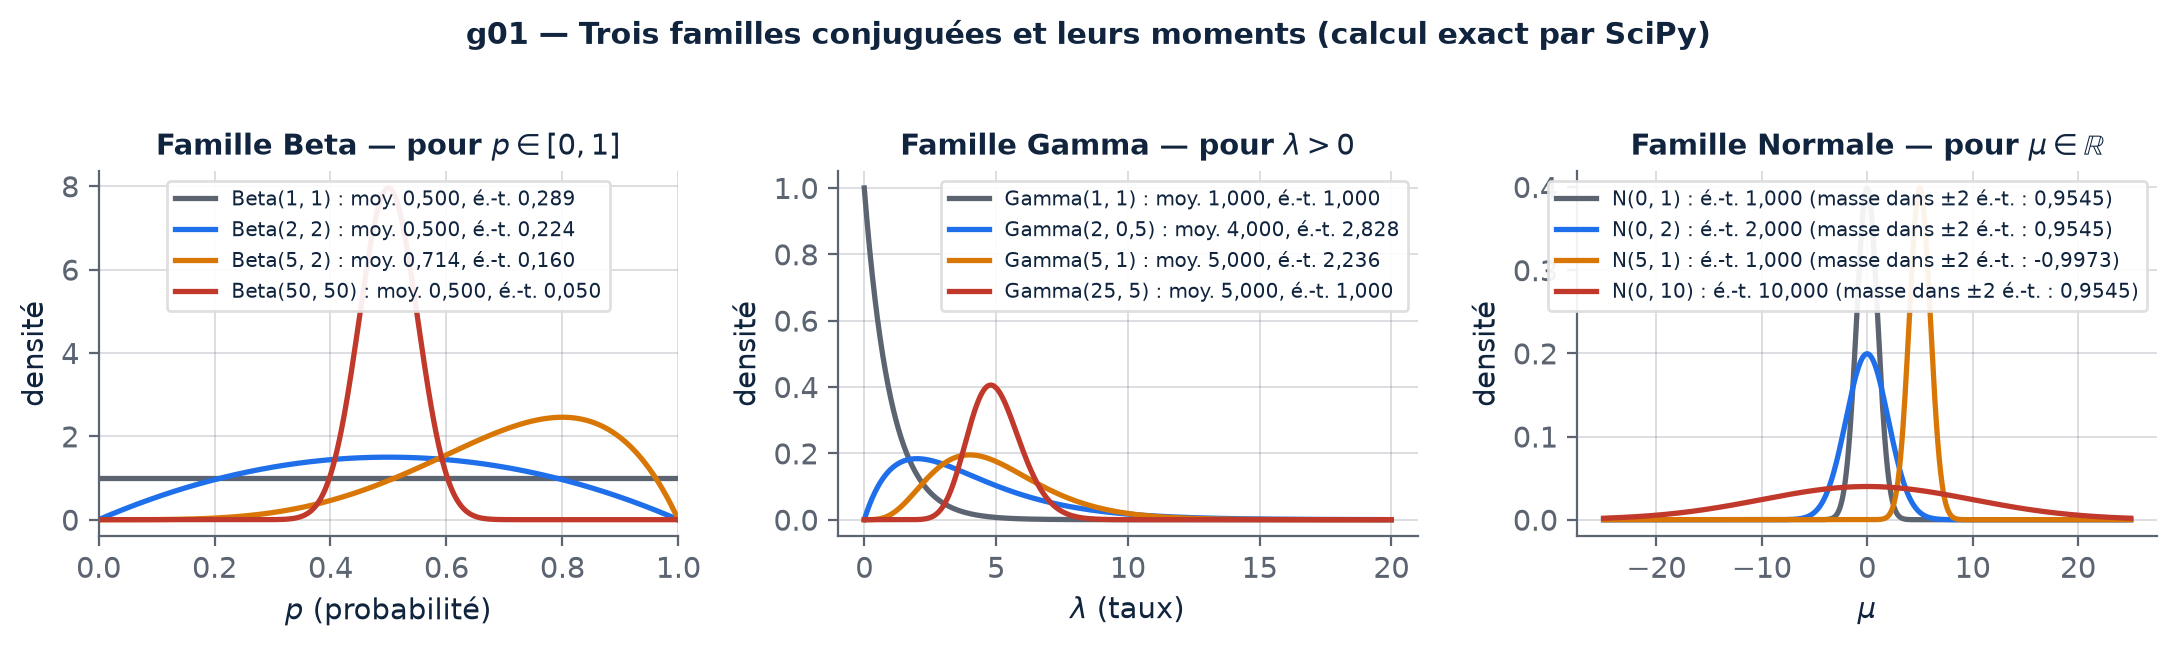
\includegraphics[width=0.74\textwidth]{g01_familles_priors.png}
\end{center}
\vspace{-1mm}
\begin{columns}[t]
\begin{column}{0.55\textwidth}
\begin{kbox}[Lire les hyperparamètres]
\begin{itemize}
  \item $\mathrm{Beta}(a,b)$ : moyenne $\frac{a}{a+b}$, écart-type
        $\sqrt{\frac{ab}{(a+b)^2(a+b+1)}}$ ; $a+b$ est la \emph{taille} de l'échantillon virtuel.
  \item $\mathrm{Gamma}(\alpha,\beta)$ : moyenne $\alpha/\beta$, écart-type
        $\sqrt{\alpha}/\beta$ ; attention au paramétrage \emph{rate} contre \emph{scale}.
  \item $\N(\mu_0,\tau^2)$ : la précision $1/\tau^2$ est l'information apportée.
\end{itemize}
\end{kbox}
\end{column}
\begin{column}{0.42\textwidth}
\begin{ebox}[Valeurs calculées (SciPy)]
$\mathrm{Beta}(1,1)$ : é.-t. $0{,}2887$ \;|\; $\mathrm{Beta}(2,2)$ : $0{,}2236$ \;|\;
$\mathrm{Beta}(50,50)$ : $0{,}0498$.\\
$\mathrm{Gamma}(1,1)$ : é.-t. $1{,}000$ \;|\; $\mathrm{Gamma}(25,5)$ : $0{,}200$\\
$= \sqrt{\alpha}/\beta = 5/5$ : resserrer un prior ne change pas sa moyenne.
\end{ebox}
\end{column}
\end{columns}
\end{frame}

% ---------------------------------------------------------------- 7
% [split]
\begin{frame}{Beta-Binomial : le cas d'école de Challenger}
\begin{center}
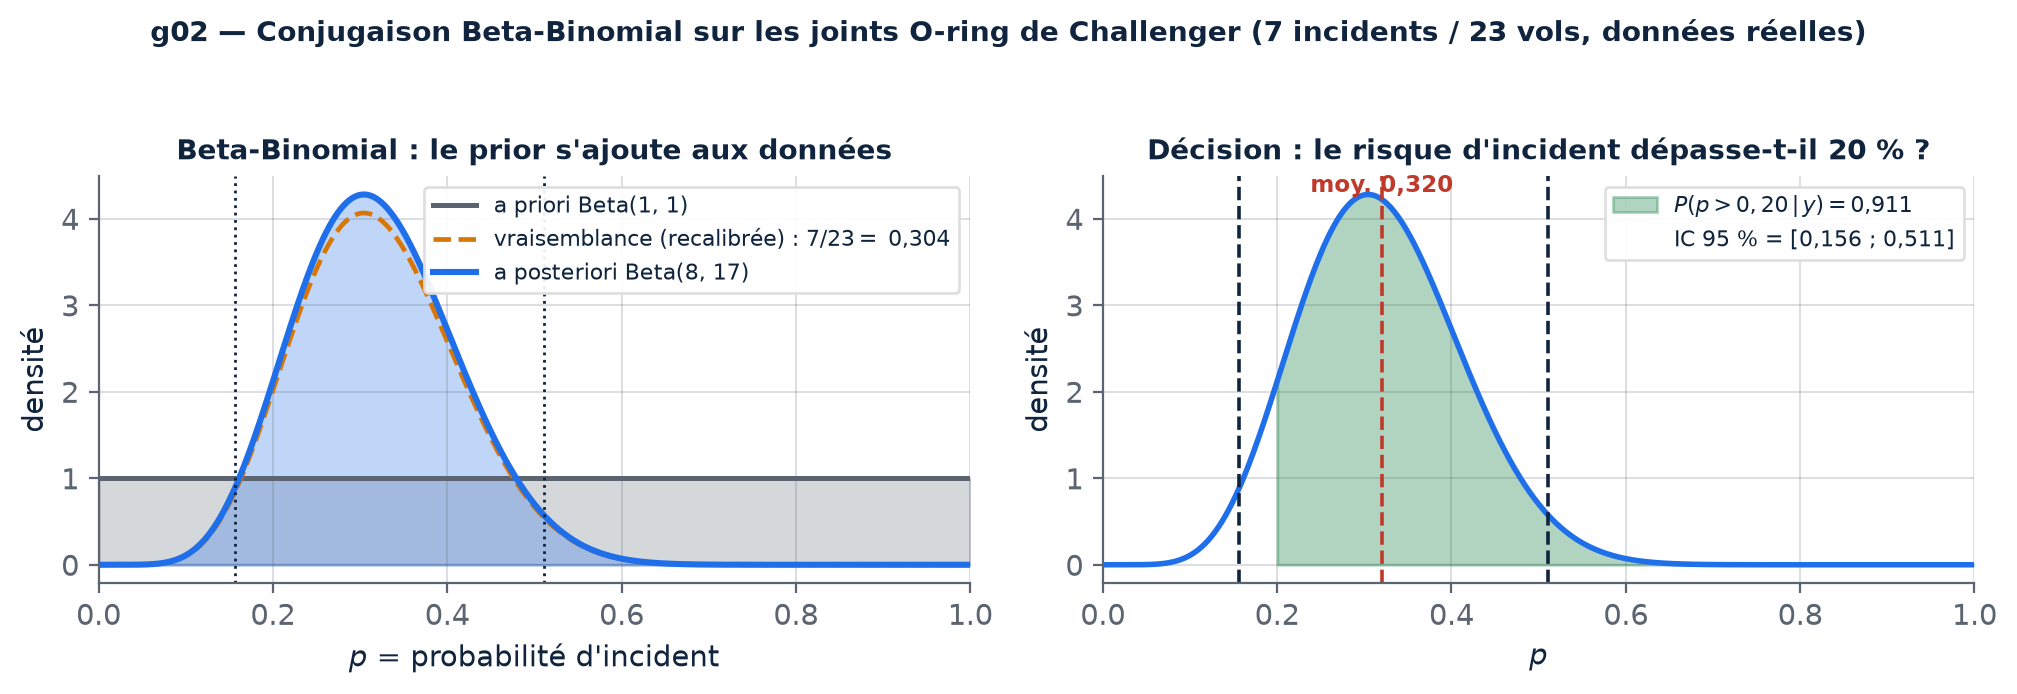
\includegraphics[width=\textwidth]{g02_conjugue_beta_binomial.png}
\end{center}
\end{frame}

% [split]
% [suite]
\begin{frame}{Beta-Binomial : le cas d'école de Challenger}
% [rogna]
\small
\begin{columns}[t]
\begin{column}{0.45\textwidth}
\begin{ebox}[Données réelles (Challenger)]
23 vols de la navette avant la catastrophe : \textbf{7 vols} présentent une
dégradation thermique des joints O-ring. Modèle :
\[
p \sim \mathrm{Beta}(1,1), \qquad k \given p \sim \mathrm{Bin}(23, p)
\]
Posterior conjugué : $\mathrm{Beta}(1+7,\,1+23-7) = \mathbf{Beta(8,17)}$.
\end{ebox}
\begin{solbox}[Résultats exécutés]
\begin{itemize}
  \item Moyenne a posteriori $\mathbf{0{,}320}$, écart-type $0{,}0915$
  \item IC 95 \% : $[0{,}156 \,;\, 0{,}511]$
  \item $P(p > 0{,}20 \given y) = \mathbf{0{,}911}$ : la question décisionnelle
  \item $P(p > 0{,}50 \given y) = 0{,}032$
\end{itemize}
\end{solbox}
\end{column}
\end{columns}
\vspace{1mm}
\end{frame}

% [suite]
\begin{frame}{Beta-Binomial : le cas d'école de Challenger (suite)}
\begin{wbox}[Le prior d'ingénieur change la conclusion]
Avec l'avis d'expert « un joint qui casse dans 1 vol sur 40 » encodé en
$\mathrm{Beta}(1{,}3,\,50)$ : posterior Beta$(8{,}3,\,66)$, moyenne
\textbf{0,112} et IC 95 \% $[0{,}051 \,;\, 0{,}192]$. Même données,
conclusion d'un facteur 3 près : \textbf{le prior doit être écrit et défendu}.
\end{wbox}
\end{frame}

% ---------------------------------------------------------------- 8
% [split]
\begin{frame}{Gamma-Poisson : le comptage de particules alpha (1910)}
\begin{center}
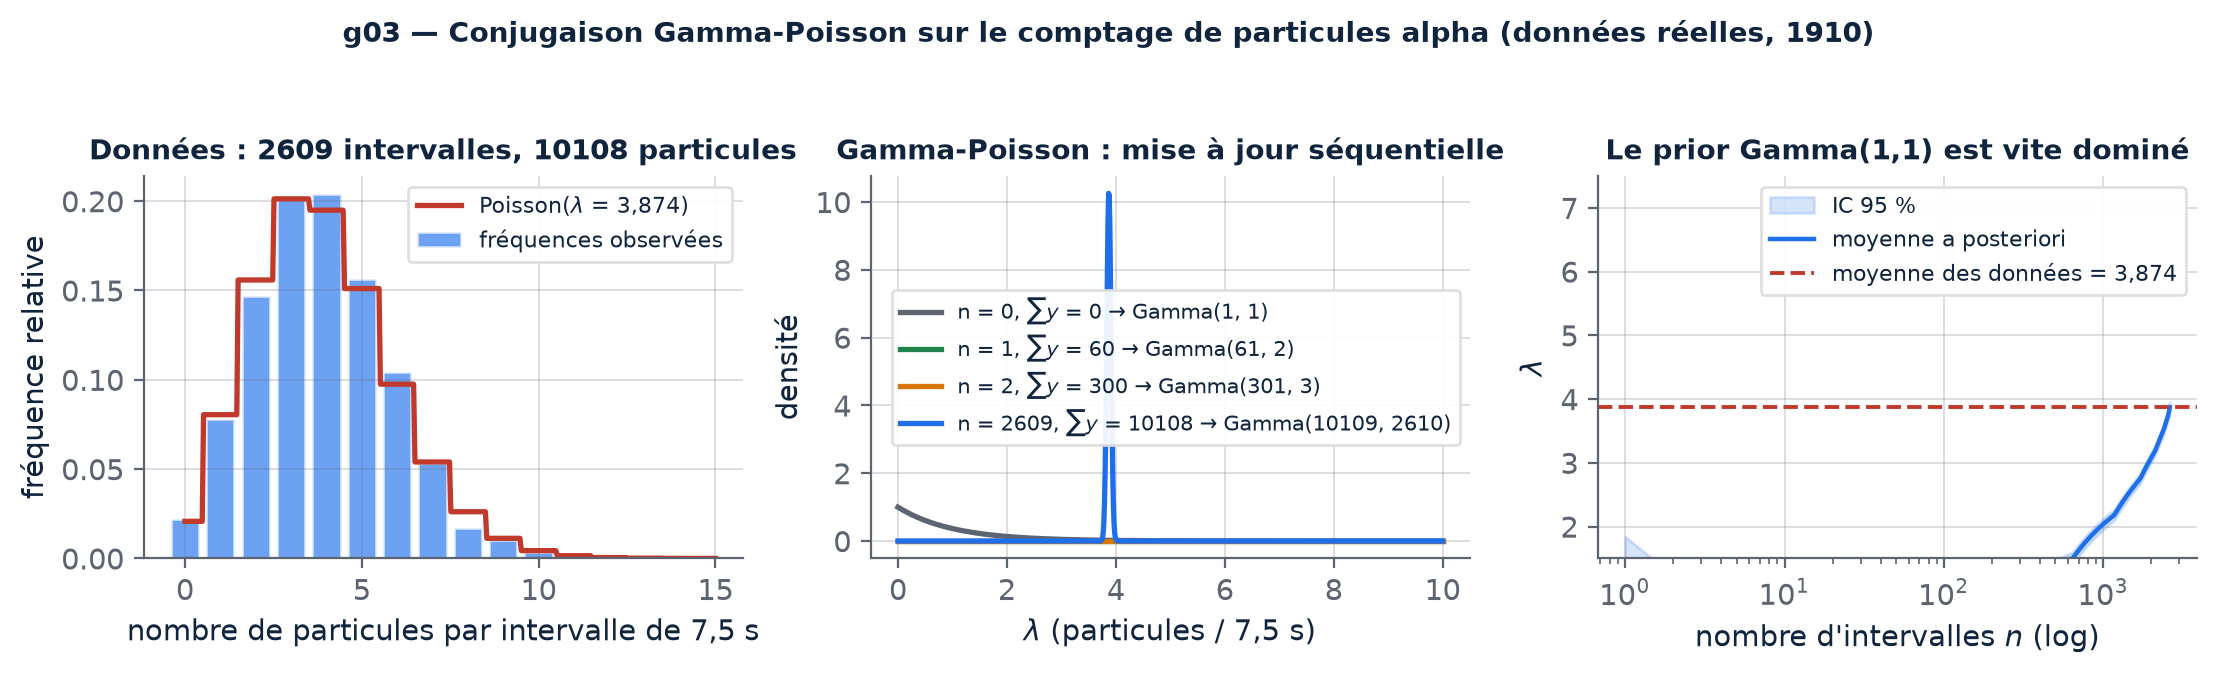
\includegraphics[width=\textwidth]{g03_conjugue_gamma_poisson.png}
\end{center}
\end{frame}

% [split]
% [suite]
% [suite5]
\begin{frame}{Gamma-Poisson : le comptage de particules alpha (1910)}
\begin{columns}[t]
\begin{column}{0.44\textwidth}
\begin{ebox}[Données réelles (Rutherford \& Geiger)]
Un compteur Geiger observe des particules alpha pendant des intervalles de 7,5 s.
Table de fréquences exploitée par le script :
\begin{itemize}
  \item $2\,609$ intervalles observés
  \item $10\,108$ particules comptées au total
  \item moyenne empirique $\bar y = \mathbf{3{,}8743}$
\end{itemize}
Modèle : $y_i \given \lambda \sim \mathrm{Poisson}(\lambda)$, prior $\mathrm{Gamma}(1,1)$.
\end{ebox}
\end{column}
\end{columns}
\vspace{1mm}
\end{frame}

% [suite5]
\begin{frame}{Gamma-Poisson : le comptage de particules alpha (1910) (suite)}
\begin{solbox}[Posterior conjugué]
\[
\mathrm{Gamma}\!\Big(1 + \sum_i y_i,\; 1 + n\Big)
= \mathrm{Gamma}(10\,109,\; 2\,610)
\]
moyenne $\mathbf{3{,}8732}$, écart-type $0{,}0385$, IC 95 \%
$[3{,}798 \,;\, 3{,}949]$.
\end{solbox}
\end{frame}

% [suite]
\begin{frame}{Gamma-Poisson : le comptage de particules alpha (1910) (suite)}
\begin{kbox}[Ce que la figure du milieu montre]
À droite, le prior ne pèse que $\frac{1}{1+n}$ : dès $n \approx 10$ intervalles
il est effacé. C'est la situation typique de la \textbf{détection de fraude} ou du
\textbf{comptage de défauts} : beaucoup d'observations, prior peu influent,
mise à jour séquentielle naturelle (on peut streamer : chaque nouveau compte
ajoute simplement 1 à $\alpha$ et 1 à $\beta$).
\end{kbox}
\end{frame}

% ---------------------------------------------------------------- 9
% [split]
\begin{frame}{Normal-Normal : une école, un bruit, un prior défendable}
\begin{center}
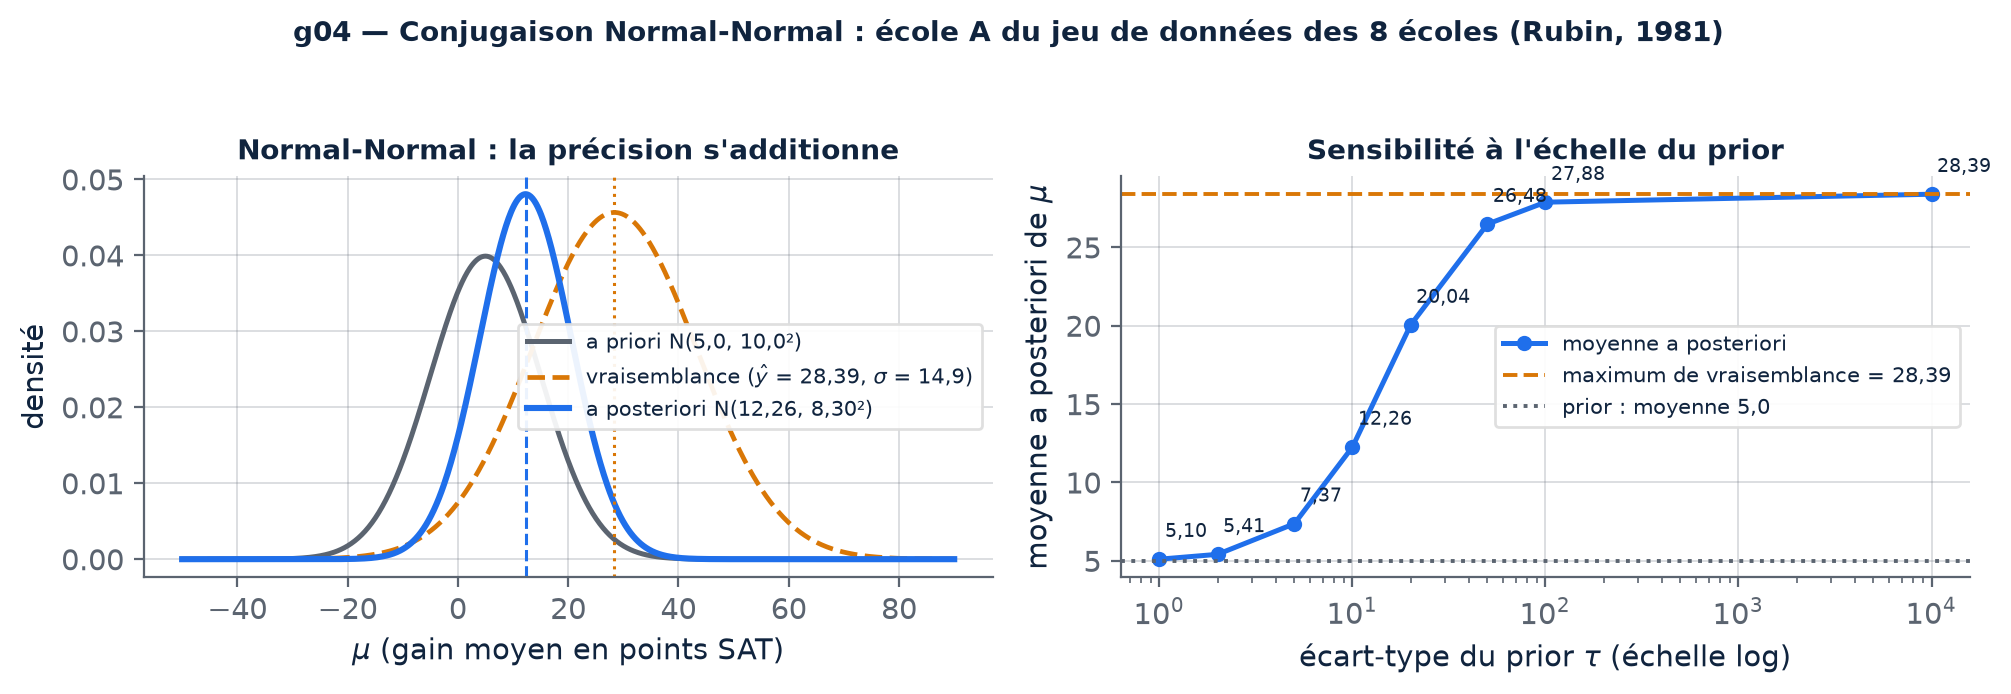
\includegraphics[width=\textwidth]{g04_conjugue_normal_normal.png}
\end{center}
\end{frame}

% [split]
% [suite5]
\begin{frame}{Normal-Normal : une école, un bruit, un prior défendable}
% [rogna]
\small
\begin{columns}[t]
\begin{column}{0.45\textwidth}
\begin{ebox}[Données réelles (Rubin, 1981)]
Le programme de préparation au SAT de l'école A est estimé à
$\hat y = 28{,}39$ points avec une erreur standard connue $\sigma = 14{,}9$.
Prior \emph{faiblement informatif} : $\mu \sim \N(5, 10^2)$.
\end{ebox}
\begin{solbox}[Posterior exact]
$\mu \given y \sim \N(12{,}2642,\; 8{,}3033^2)$, IC 95 \%
$[-4{,}01 \,;\, 28{,}54]$.\\[1mm]
Le posterior \textbf{contracte} l'estimation d'un facteur
$\mathbf{0{,}432}$ vers le prior.
\end{solbox}
\end{column}
\end{columns}
\end{frame}

% [suite5]
\begin{frame}{Normal-Normal : une école, un bruit, un prior défendable (suite)}
\begin{kbox}[Le levier est $\tau$, pas $\mu_0$]
$\tau = 1 \to 5{,}105$ ; $\tau = 5 \to 7{,}367$ ;
$\tau = 10 \to 12{,}264$ ; $\tau = 50 \to 26{,}482$ ; $\tau = 10^4 \to 28{,}390$
(le maximum de vraisemblance). Choisir $\tau$ \emph{calibre l'information}
apportée par l'expert.
\end{kbox}
\end{frame}

% ---------------------------------------------------------------- 10
% [split]
\begin{frame}{Dirichlet-Multinomial : les 556 pois de Mendel}
\begin{center}
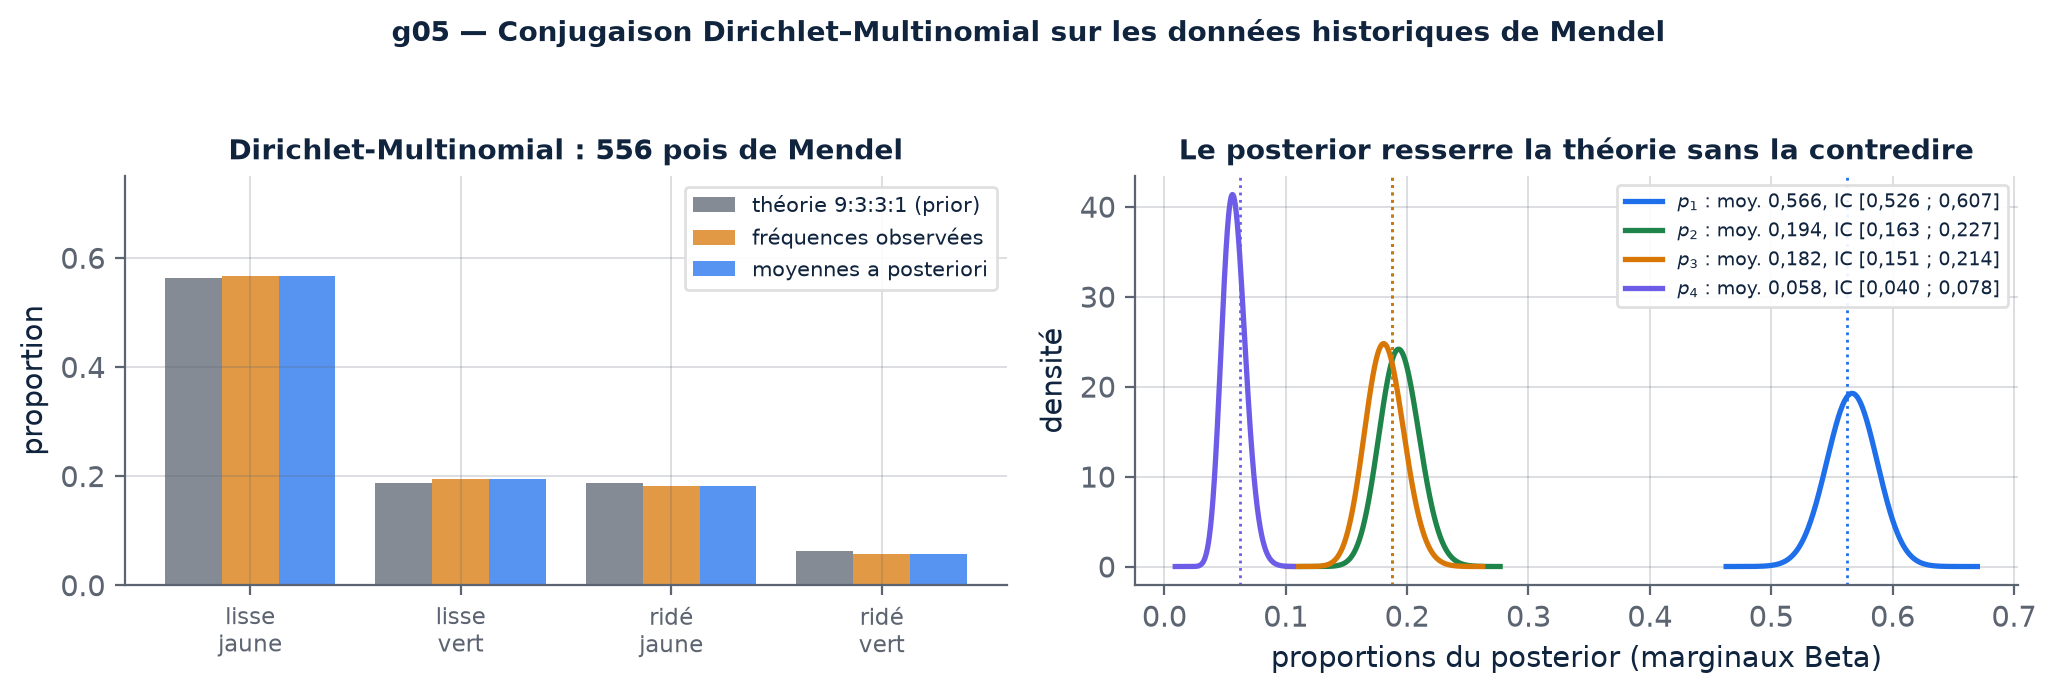
\includegraphics[width=\textwidth]{g05_conjugue_dirichlet_multinomial.png}
\end{center}
\end{frame}

% [split]
% [suite5]
\begin{frame}{Dirichlet-Multinomial : les 556 pois de Mendel}
% [rogna]
\small
\begin{columns}[t]
\begin{column}{0.45\textwidth}
\begin{ebox}[Données (Mendel, 1865)]
556 pois répartis en quatre phénotypes : lisse-jaune \textbf{315}, lisse-vert
\textbf{108}, ridé-jaune \textbf{101}, ridé-vert \textbf{32}. La théorie de Mendel
donne les proportions $9{:}3{:}3{:}1 = (0{,}5625 ; 0{,}1875 ; 0{,}1875 ; 0{,}0625)$.
\end{ebox}
\begin{solbox}[La théorie entre comme a priori]
$\alpha_0 = (9, 3, 3, 1)$ \;$\to$\;
$\mathrm{Dirichlet}(9+315,\,3+108,\,3+101,\,1+32) = \mathbf{Dirichlet(324, 111, 104, 33)}$
\end{solbox}
\end{column}
\end{columns}
\vspace{1mm}
\centering\small
\textbf{Lecture} — trois intervalles sur quatre contiennent la prédiction théorique :
le posterior \emph{resserre} la théorie sans la contredire. C'est exactement l'usage
d'une loi a priori comme \emph{hypothèse de travail falsifiable}.
\end{frame}

% [suite5]
\begin{frame}{Dirichlet-Multinomial : les 556 pois de Mendel (suite)}
\begin{kbox}[Les quatre marginaux]
$p_1$ : $0{,}5664$ \;$[0{,}5257;0{,}6068]$ (théorie $0{,}5625$) \;/\;
$p_2$ : $0{,}1941$ \;$[0{,}1627;0{,}2274]$ ($0{,}1875$) \\
$p_3$ : $0{,}1818$ \;$[0{,}1513;0{,}2144]$ \;/\;
$p_4$ : $0{,}0577$ \;$[0{,}0401;0{,}0782]$
\end{kbox}
\end{frame}

% ---------------------------------------------------------------- 11
% [rogna]
% [rogna]
% [rogna]
% [split]
\begin{frame}{Vue d'ensemble : quatre couples, un même mécanisme}
\begin{center}
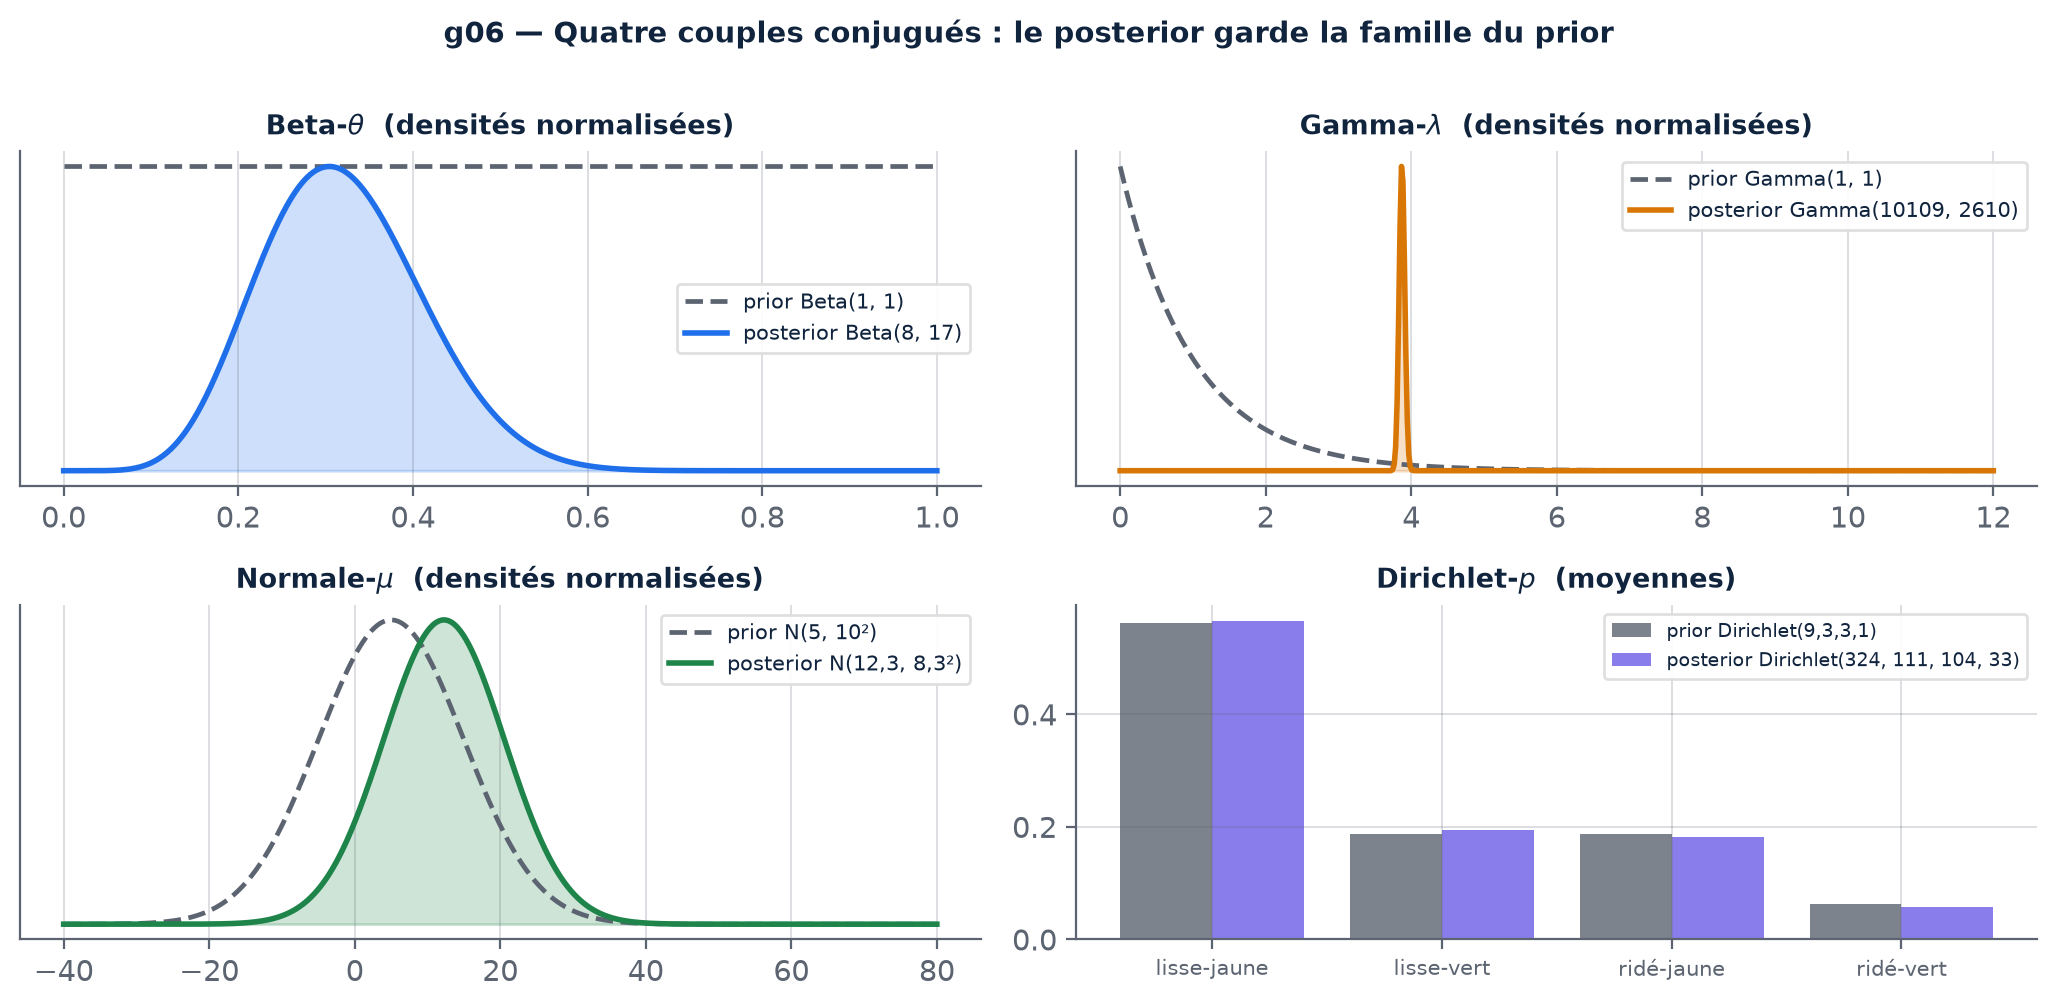
\includegraphics[width=.86\textwidth]{g06_quatre_trios.png}
\end{center}
\end{frame}

% [split]
\begin{frame}{Vue d'ensemble : quatre couples, un même mécanisme}

\vspace{-4mm}
\begin{columns}[t]
\begin{column}{0.48\textwidth}
\begin{kbox}[Ce que la figure prouve]
Dans les quatre cas, le posterior appartient à la \textbf{même famille} que le
prior : Beta $\to$ Beta, Gamma $\to$ Gamma, Normale $\to$ Normale,
Dirichlet $\to$ Dirichlet. Seuls les \emph{hyperparamètres} ont changé, et
toujours d'une seule manière : on a ajouté les données.
\end{kbox}
\end{column}
\begin{column}{0.48\textwidth}
\begin{ebox}[Le test à refaire en examen]
Écrire un modèle (vraisemblance + prior), dériver le noyau du posterior,
identifier la famille et ses paramètres, puis donner moyenne, mode et
intervalle de crédibilité. Quatre modèles au programme, cinq minutes chacun.
\end{ebox}
\end{column}
\end{columns}
\end{frame}

% ---------------------------------------------------------------- 12
\begin{frame}[fragile]{Vérification : le même posterior par PyMC (10 lignes)}
\begin{columns}[t]
\begin{column}{0.53\textwidth}
\begin{codebox}[src/fig\_ch2b\_pymc.py — modèle Beta-Binomial]
\begin{lstlisting}
import pymc as pm, arviz as az
import numpy as np

n_vols, k_incidents = 23, 7      # donnees reelles

with pm.Model() as m:
    p = pm.Beta("p", alpha=1, beta=1)   # prior uniforme
    pm.Binomial("y", n=n_vols, p=p,
                observed=k_incidents)

    idata = pm.sample(draws=2000, tune=1000,
                      chains=2, cores=1,
                      random_seed=42)

echantillons = idata.posterior["p"].values.ravel()
print(echantillons.mean())
print(np.percentile(echantillons, [2.5, 97.5]))
\end{lstlisting}
\end{codebox}
\end{column}
\begin{column}{0.44\textwidth}
\begin{kbox}[Le contrat de l'échantillonneur]
Aucune conjugaison, aucune dérivée à la main : on \emph{décrit} le modèle et
NUTS explore le posterior. Le prix est le diagnostic : $\hat R$, taille
d'échantillon efficace, autocorrélation.
\end{kbox}
\begin{solbox}[Résultat exécuté sur CPU]
Moyenne $0{,}3196$ \;;\; IC 95 \% $[0{,}1536 \,;\, 0{,}5138]$ \;;\;
$\hat R = 1{,}0016$ \;;\; ESS $\approx 1\,719$ \;;\; $41{,}2$~s.
\end{solbox}
\end{column}
\end{columns}
\end{frame}

% ---------------------------------------------------------------- 13
% [rogna]
% [rogna]
% [rogna]
\begin{frame}{Analytique contre échantillonnage : le match nul attendu}
\begin{center}
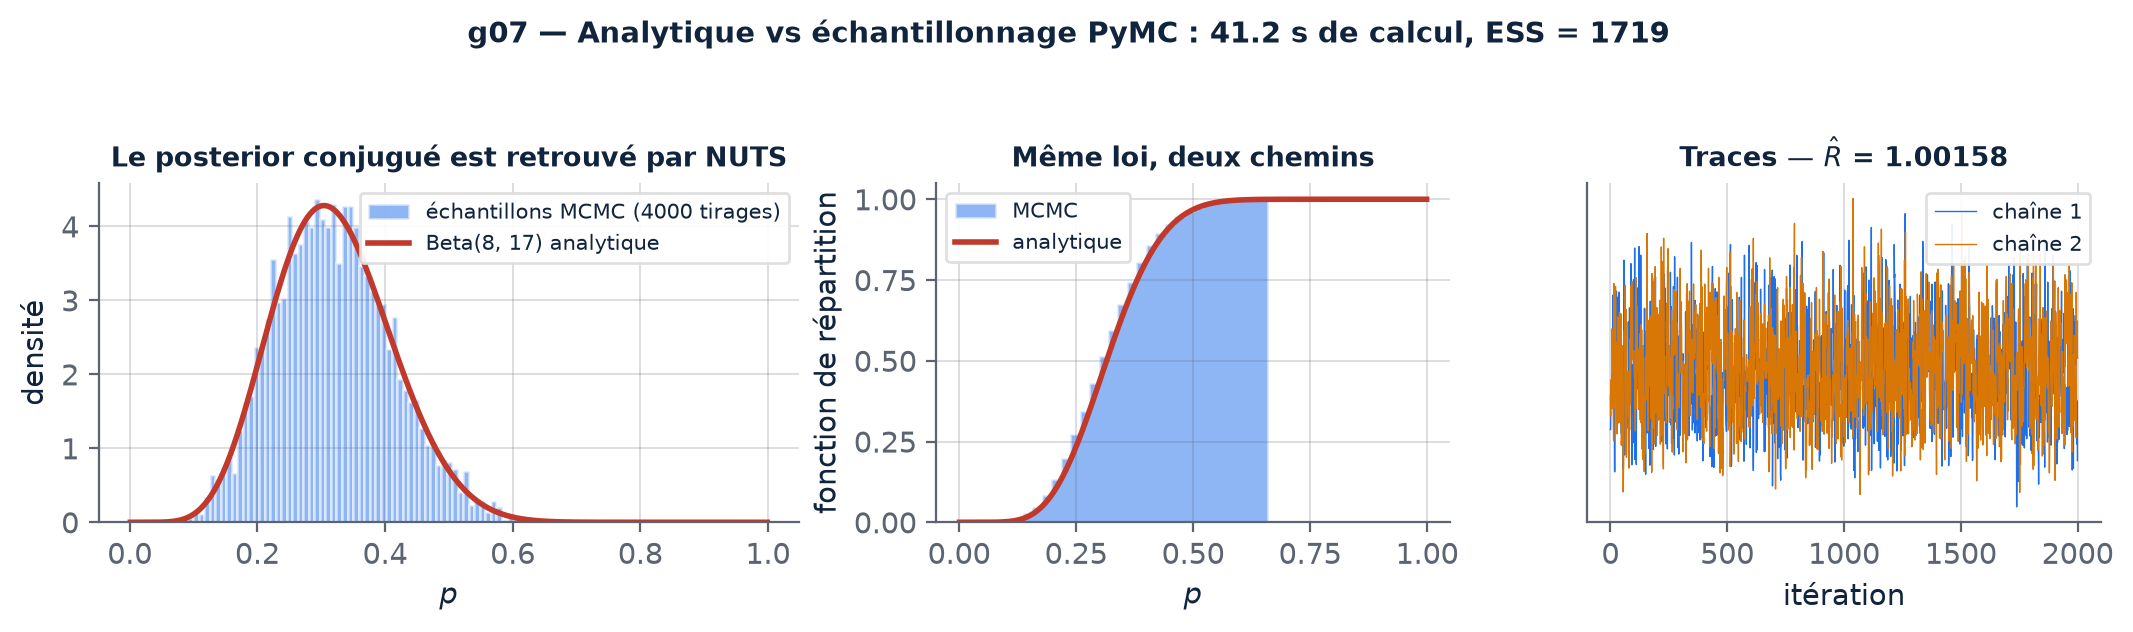
\includegraphics[width=.88\textwidth]{g07_analytique_vs_pymc.png}
\end{center}
\vspace{-1mm}
\begin{columns}[t]
\begin{column}{0.52\textwidth}
\begin{solbox}[Comparaison numérique]
\begin{tabular}{@{}lcc@{}}
\toprule
& \textbf{Exact} & \textbf{MCMC} \\
\midrule
loi du posterior & Beta$(8,17)$ & échantillons \\
moyenne & $0{,}3200$ & $0{,}3196$ \\
IC 95 \% bas & $0{,}1563$ & $0{,}1536$ \\
IC 95 \% haut & $0{,}5109$ & $0{,}5138$ \\
\bottomrule
\end{tabular}
\end{solbox}
\end{column}
\begin{column}{0.45\textwidth}
\begin{kbox}[La règle professionnelle]
On \textbf{valide toujours} un échantillonneur sur un cas conjugué avant de lui
confier un modèle sans forme close : ici $41{,}2$~s de calcul pour un résultat
déjà connu exactement. Les sections 2.2 à 2.4 n'utilisent que des cas où la
vérité est calculable.
\end{kbox}
\end{column}
\end{columns}
\end{frame}

% ---------------------------------------------------------------- 14
\begin{frame}{Lire un prior comme un échantillon virtuel}
\begin{ebox}[L'équation des débats sur les priors]
Pour le modèle Beta-Binomial, la moyenne a posteriori est une \textbf{moyenne pondérée}
entre le prior et les données :
\[
\underbrace{\hat p_{\post}}_{\text{posterior}}=
\underbrace{w}_{\text{poids du prior}} \cdot \underbrace{\frac{a}{a+b}}_{\text{moyenne du prior}}
\;+\;(1-w)\cdot \underbrace{\frac{k}{n}}_{\text{données}},
\qquad w = \frac{a+b}{a+b+n}
\]
\end{ebox}
\vspace{1mm}
\centering
\begin{tabular}{@{}p{1.8cm}p{0.9cm}p{1.3cm}p{1.8cm}p{2.3cm}p{3.9cm}@{}}
\toprule
\textbf{A priori} & $a+b$ & $w$ & \textbf{moy. post.} & \textbf{IC 95 \%} & \textbf{verdict} \\
\midrule
Beta$(1,1)$ & 2 & 0,080 & 0,3200 & $[0{,}156;0{,}511]$ & les données décident \\
Beta$(2,2)$ & 4 & 0,148 & 0,3333 & $[0{,}172;0{,}518]$ & presque neutre \\
Beta$(5,3)$ & 8 & 0,258 & 0,3871 & $[0{,}227;0{,}561]$ & avis marqué \\
Beta$(1{,}3;50)$ & 51,3 & \textbf{0,690} & 0,1117 & $[0{,}051;0{,}192]$ & \textbf{le prior domine} \\
\bottomrule
\end{tabular}
\vspace{1.5mm}
\begin{wbox}[Le piège des pseudo-observations]
Un $\mathrm{Beta}(50,50)$ encode \textbf{98} observations virtuelles et un
$w = 0{,}813$ face à 23 vols réels : convertir tout prior en \emph{taille
d'échantillon équivalente} avant de le dire neutre.
\end{wbox}
\end{frame}

% ---------------------------------------------------------------- 15
\begin{frame}{Quiz 1 — conjugaison en quatre questions}
\begin{qbox}[Question 3 -- Mise à jour]
\textbf{1.} On suppose $y_1,\dots,y_n \sim \mathrm{Poisson}(\lambda)$ et
$\lambda \sim \mathrm{Gamma}(2, 1)$. Après $n = 12$ et $\sum y_i = 48$,
quels sont les paramètres du posterior ? \\[1mm]
\textbf{2.} Même modèle, mais $\sum y_i = 48$ et $n = 240$ : quel prior pèse
le plus, et pourquoi ? \\[1mm]
\textbf{3.} Pour une proportion $p$, quels hyperparamètres encode un avis « autour
de 0,3, plutôt précis » ? Et un avis « entre 0,1 et 0,5 sans plus » ? \\[1mm]
\textbf{4.} Un collègue écrit : « prior Beta$(0{,}5;0{,}5)$ = pas d'information ».
A-t-il raison ?
\vspace{2mm}

\textcolor{byBlue}{\textbf{Réponses :}}
\textbf{1.} $\mathrm{Gamma}(2+48,\,1+12) = \mathrm{Gamma}(50,13)$, moyenne
$3{,}846$. \quad
\textbf{2.} Poids $w = 3/(3+240) = 0{,}012$ : le prior est écrasé (vs $3/15 = 0{,}20$). \quad
\textbf{3.} Beta$(15,35)$ (moy. 0,3000, é.-t. 0,0642) contre Beta$(2,4)$ (moy. 0,3333, é.-t. 0,1782). \quad
\textbf{4.} Non : c'est le prior de \textbf{Jeffreys}, le moins informatif qui garde
une invariance ; mais il favorise 0 et 1, ce qui est une information (section 2.2).
\end{qbox}
\end{frame}

% ---------------------------------------------------------------- 16
\begin{frame}{Activité guidée — dériver un posterior à la main (8 min)}
% [rogna]
\small
\begin{abox}[Consigne, par binôme]
On observe une pièce lancée $n = 10$ fois, donnant $k = 3$ faces.
Prior : $\theta \sim \mathrm{Beta}(2,2)$.
\begin{enumerate}
  \item Écrire $p(\theta)$ et le noyau de la vraisemblance.
  \item Multiplier, puis \textbf{identifier} les paramètres du posterior.
  \item Calculer la moyenne a posteriori à la main, puis vérifier avec le script.
  \item Répondre : $P(\theta > 0{,}5 \given y)$ est-elle supérieure à 0,2 ?
\end{enumerate}
\end{abox}
\vspace{1mm}
\begin{columns}[t]
\begin{column}{0.55\textwidth}
\begin{solbox}[Correction détaillée]
\[
p(\theta) \propto \theta^{1}(1-\theta)^{1}, \qquad
p(y \given \theta) \propto \theta^{3}(1-\theta)^{7}
\]
\[
p(\theta \given y) \propto \theta^{4}(1-\theta)^{8}
= \mathrm{Beta}(5, 9)
\]
Moyenne : $\frac{5}{5+9} = \mathbf{0{,}3571}$.
Poids du prior : $w = \frac{2+2}{4+10} = 0{,}2857$.
Vérification directe par la formule pondérée :
$0{,}2857 \times 0{,}5 + 0{,}7143 \times 0{,}3 = 0{,}3571$.
\end{solbox}
\end{column}
\begin{column}{0.42\textwidth}
\begin{ebox}[Contrôle par la loi exacte]
$\mathrm{Beta}(5,9)$ : $P(\theta > 0{,}5) = 0{,}1334$ (calcul SciPy).
La réponse au point 4 est donc \textbf{non} : malgré $k/n = 0{,}3$ et un prior
centré sur 0,5, la probabilité que la pièce soit biaisée vers face reste faible.
La conclusion s'énonce toujours avec la question posée : « biaisée vers
\emph{face} », pas « truquée ».
\end{ebox}
\end{column}
\end{columns}
\end{frame}

% ---------------------------------------------------------------- 17
\begin{frame}{Synthèse 2.1 — ce qu'il faut avoir retenu}
% [rogna]
\footnotesize
\begin{kbox}[Les cinq acquis de la conjugaison]
\begin{enumerate}
  \item Le posterior s'obtient en \textbf{reconnaissant un noyau} : la constante de
        normalisation ne se calcule jamais.
  \item Les quatre couples (Beta-Binomial, Gamma-Poisson, Normal-Normal,
        Dirichlet-Multinomial) couvrent l'essentiel des cas d'usage.
  \item Les hyperparamètres se lisent comme des \textbf{comptes de données
        virtuelles} : $w = \frac{a+b}{a+b+n}$ mesure la force du prior.
  \item La conjugaison est \textbf{exacte et instantanée} : elle sert de banc
        d'essai pour les échantillonneurs du chapitre 5.
  \item Un prior informatif peut renverser une conclusion : sur Challenger, la
        moyenne passe de $0{,}320$ à $0{,}112$.
\end{enumerate}
\end{kbox}
\vspace{-2mm}
\begin{columns}[t]
\begin{column}{0.54\textwidth}
\begin{ebox}[Passerelle vers la section 2.2]
La conjugaison suppose la famille de priors choisie. La vraie question n'est donc
pas « comment calculer ? » mais « \textbf{quel prior écrire, et comment le
justifier} ? ». C'est l'objet de la section suivante.
\end{ebox}
\end{column}
\begin{column}{0.42\textwidth}
\begin{wbox}[Trois erreurs à ne plus commettre]
\warn{} confondre précision et faible influence : un prior très resserré est très
influent ; \;
\warn{} oublier que le posterior \emph{dépend} du prior ; \;
\warn{} conclure sans donner l'intervalle de crédibilité.
\end{wbox}
\end{column}
\end{columns}
\end{frame}

% =====================================================================
%  EPD-SDIA-4112 -- Statistique Bayesienne -- Master 1 SDIA
%  CHAPITRE 2 : Distributions a priori et a posteriori
%  Fichier B : sections 2.2 (choisir un a priori) et 2.3 (controles predictifs)
% =====================================================================

% ---------------------------------------------------------------- 1
% [suite]
\begin{frame}{2.2 — Qu'est-ce qu'un a priori défendable ?}
% [rogna]
\small
\begin{kbox}[Les trois niveaux d'information]
\begin{itemize}
  \item \textbf{Non informatif} — on refuse d'injecter du contenu : uniforme, Jeffreys,
        a priori de référence. Objectif : laisser les données décider.
  \item \textbf{Faiblement informatif} — on borne l'\emph{échelle} plausible sans
        affirmer de valeur centrale : $\N(0,1)$ sur une variable standardisée.
        C'est la recommandation moderne (Gelman et al.).
  \item \textbf{Informatif} — on encode une connaissance substantielle
        (essai antérieur, contrainte physique, avis d'expert).
\end{itemize}
\end{kbox}
\vspace{1mm}
\end{frame}

% [suite]
\begin{frame}{2.2 — Qu'est-ce qu'un a priori défendable ? (suite)}
\begin{columns}[t]
\begin{column}{0.55\textwidth}
\begin{ebox}[Le même chiffre, trois lectures]
La « taille » d'un prior Beta se lit dans $a+b$, le nombre d'observations virtuelles
(\textbf{calculé} dans \file{src/fig\_ch2c\_poids.py}) :
\begin{center}
\begin{tabular}{@{}lcc@{}}
\toprule
\textbf{Prior} & $a+b$ & \textbf{obs. virtuelles} \\
\midrule
Beta$(1,1)$ & 2 & 0 \\
Beta$(2,2)$ & 4 & 2 \\
Beta$(5,3)$ & 8 & 6 \\
Beta$(1{,}3;50)$ & 51,3 & 49,3 \\
Beta$(50,50)$ & 100 & \textbf{98} \\
\bottomrule
\end{tabular}
\end{center}
\end{ebox}
\end{column}
\begin{column}{0.42\textwidth}
\begin{wbox}[La question à poser à chaque fois]
« Si j'avais \textbf{98} observations et qu'elles étaient toutes dans ce sens,
écrirais-je la même chose ? » Si la réponse est non, le prior est trop fort.
Le vérifier : face aux 23 vols de Challenger, Beta$(50,50)$ pèse
$w = \frac{100}{100+23} = 0{,}813$.
\end{wbox}
\end{column}
\end{columns}
\end{frame}

% ---------------------------------------------------------------- 2
\begin{frame}{Boîte à outils : six façons d'écrire un a priori}
\centering
\renewcommand{\arraystretch}{1.25}
\small
\footnotesize\scriptsize\begin{tabular}{@{}p{2.5cm}p{3.9cm}p{1.7cm}p{3.4cm}@{}}
\toprule
\textbf{A priori} & \textbf{Définition} & \textbf{Propre ?} & \textbf{Quand l'utiliser} \\
\midrule
Uniforme & $p(\theta) \propto 1$ sur un domaine borné & oui & proportion ou taux
naturellement borné \\[1mm]
Uniforme sur $\log\theta$ & $p(\theta) \propto 1/\theta$ & non & paramètre d'échelle
positif \\[1mm]
Jeffreys & $p(\theta) \propto \sqrt{\det I(\theta)}$ & non & invariance par
reparamétrisation \\[1mm]
Référence & maximise l'information attendue & non & comparaison objective de
modèles \\[1mm]
Faiblement informatif & centré en 0, échelle fixée & oui & régression, modèles
hiérarchiques \\[1mm]
Informatif & élicitation structurée (expertise) & oui & réplication, données
rares \\[1mm]
\bottomrule
\end{tabular}
\vspace{2mm}
\begin{tcolorbox}[colback=byPurple!6,colframe=byPurple,arc=2mm,width=.94\textwidth]
\small\centering
\textbf{Aucun de ces choix n'est « neutre »} : chacun est une décision scientifique,
et c'est pour cela qu'elle doit être écrite dans le rapport d'analyse.
(Le \emph{power prior} de la section 2.4 est un traitement du \emph{désaccord} entre
données passées et présentes.)
\end{tcolorbox}
\end{frame}

% ---------------------------------------------------------------- 3
\begin{frame}{Le prior de Jeffreys : l'invariance comme principe}
% [rogna]
\footnotesize
\begin{columns}[t]
\begin{column}{0.50\textwidth}
\begin{kbox}[Deux lignes de mathématiques]
$I(\theta)$ est l'information de Fisher d'une observation :
\[
I(\theta) = -\,\E\!\left[\frac{\partial^2 \log p(y \given \theta)}{\partial \theta^2}\right],
\qquad p_{\text{Jeffreys}}(\theta) \propto \sqrt{\det I(\theta)}
\]
Cette règle est \textbf{invariante} : elle donne le même en prior pour $\lambda$ et
$1/\lambda$, ce que ne fait \emph{jamais} l'uniforme.
\end{kbox}
\begin{ebox}[Trois cas calculés dans le cours]
\begin{itemize}
  \item Binomiale : $I(p) = \frac{1}{p(1-p)} \Rightarrow \mathrm{Beta}(1/2, 1/2)$
  \item Poisson : $I(\lambda) = 1/\lambda \Rightarrow \mathrm{Gamma}(1/2, 0)$ (impropre)
  \item Normale, $\mu$ inconnue, $\sigma$ connu : $I(\mu) = 1/\sigma^2 \Rightarrow$
        \textbf{uniforme} (donc impropre si $\mu \in \R$)
\end{itemize}
\end{ebox}
\end{column}
\begin{column}{0.47\textwidth}
\begin{solbox}[Vérification numérique exécutée]
Sur une grille de $20\,001$ valeurs de $p$ :
\[
\begin{aligned}
\max_p\Bigl|\frac{\sqrt{I(p)}}{\max\sqrt{I}}
&- \frac{\text{noyau Beta}(1/2,1/2)}{\max}\Bigr|\\[1mm]
&= 1{,}67 \cdot 10^{-16}
\end{aligned}
\]
c'est-à-dire une identité exacte, à l'erreur machine près.\\
$B(1/2, 1/2) = \pi = 3{,}141593$ (écart numérique avec $\pi$ : $4{,}4 \cdot 10^{-16}$).
\end{solbox}
\begin{wbox}[Le prix à payer]
Jeffreys \textbf{favorise les extrêmes} : $P(p < 0{,}1) = 0{,}2048$ pour
Beta$(0{,}5;0{,}5)$ contre $0{,}1000$ pour l'uniforme. Ce n'est pas de l'ignorance,
c'est une information (les paramètres proches de la frontière sont plus « vrais »
sous reparamétrisation).
\end{wbox}
\end{column}
\end{columns}
\end{frame}

% ---------------------------------------------------------------- 4
\begin{frame}{Jeffreys au banc d'essai : les petits échantillons}
\begin{center}
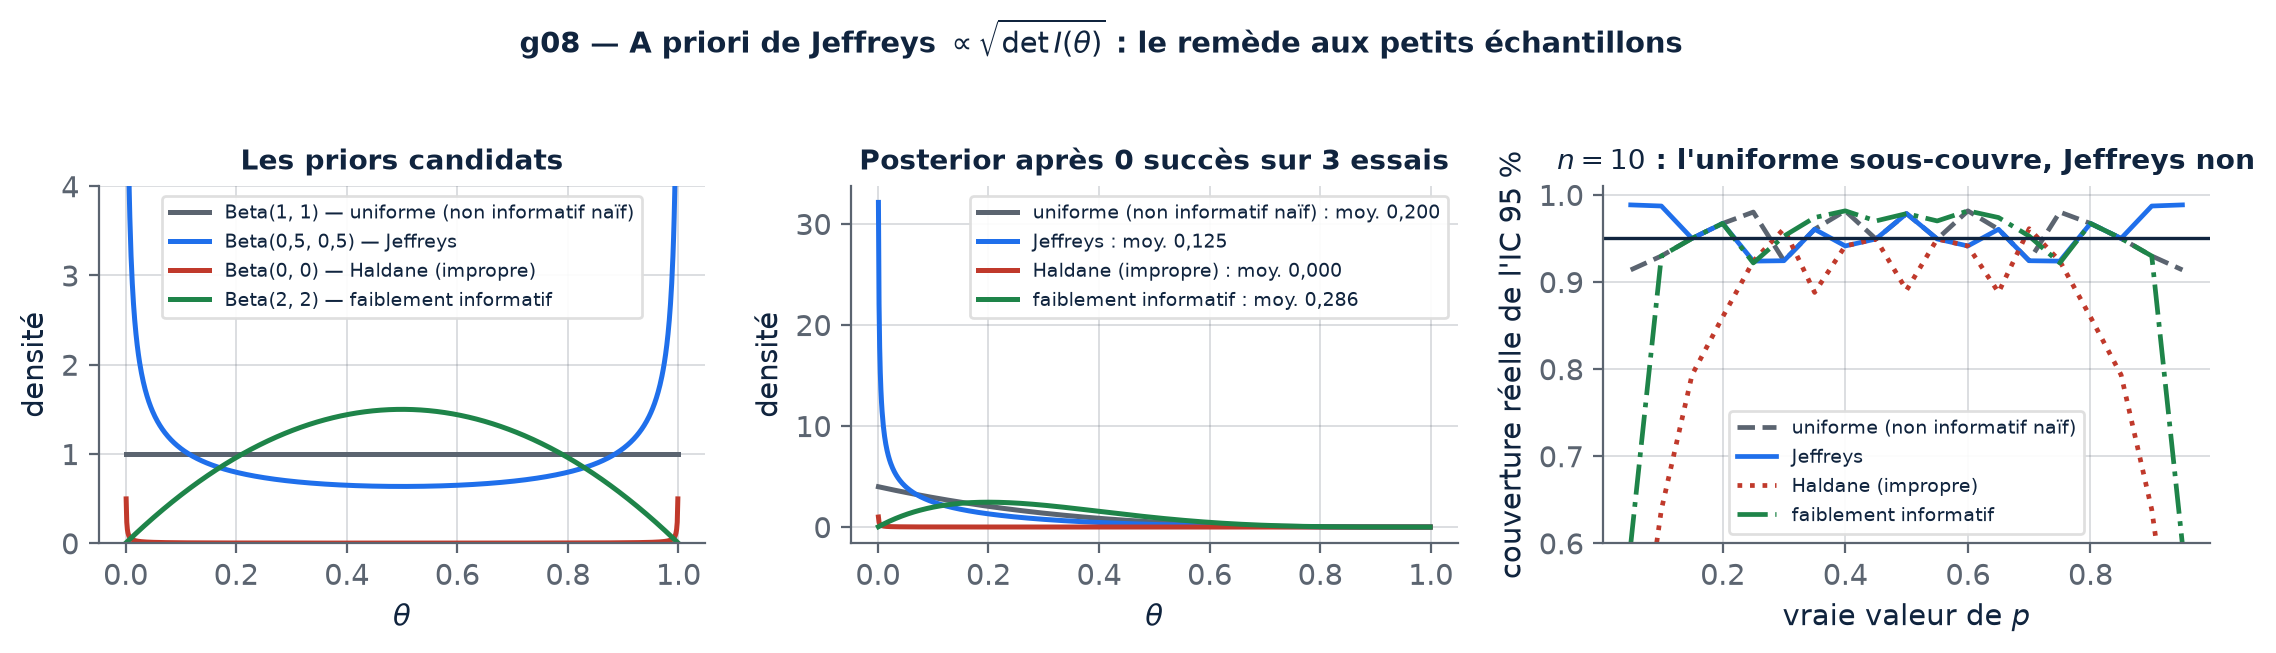
\includegraphics[width=0.90\textwidth]{g08_jeffreys.png}
\end{center}
\vspace{-4mm}
\begin{columns}[t]
\begin{column}{0.55\textwidth}
\begin{ebox}[Cas limite : $0$ succès sur $3$ essais]
\begin{tabular}{@{}lcc@{}}
\toprule
\textbf{Prior} & \textbf{moyenne} & \textbf{IC 95 \%} \\
\midrule
Uniforme Beta$(1,1)$ & 0,200 & $[0{,}0063 \,;\, 0{,}6024]$ \\
Jeffreys Beta$(0{,}5;0{,}5)$ & \textbf{0,125} & $[0{,}0002 \,;\, 0{,}5356]$ \\
Haldane Beta$(0,0)$ & 0,0003 & $[0{,}0000 \,;\, 0{,}0000]$ \\
Beta$(2,2)$ (faiblement inf.) & 0,2857 & $[0{,}0433 \,;\, 0{,}6412]$ \\
\bottomrule
\end{tabular}
\end{ebox}
\end{column}
\begin{column}{0.42\textwidth}
\begin{kbox}[La mesure qui départage]
Couverture réelle de l'IC 95 \% pour $n = 10$ (somme exacte sur les $2^{10}$
échantillons possibles) : uniforme $\in [0{,}914 ; 0{,}982]$, Jeffreys
$\in [0{,}924 ; 0{,}989]$, Beta$(2,2)$ $\in [0{,}599 ; 0{,}982]$.
Jeffreys est le plus \emph{honnête} aux valeurs extrêmes ; Haldane s'effondre
jusqu'à $0{,}390$.
\end{kbox}
\end{column}
\end{columns}
\end{frame}

% ---------------------------------------------------------------- 5
\begin{frame}{Propre contre impropre : la ligne rouge}
\begin{columns}[t]
\begin{column}{0.49\textwidth}
\begin{ebox}[Définitions]
Un prior est \textbf{propre} si $\int p(\theta)\,\mathrm{d}\theta = 1$.
Il est \textbf{impropre} si l'intégrale diverge, tout en restant utilisable
\emph{formellement} : l'uniforme sur $\R$, Beta$(0,0)$, $\mathrm{Gamma}(1/2,0)$,
$1/\sigma$.
\end{ebox}
\begin{solbox}[Ce qui se passe vraiment]
Un prior impropre est acceptable \textbf{si et seulement si} le posterior est
propre : c'est le cas de Haldane Beta$(0,0)$ face à $0$ succès sur $3$ essais
(posterior Beta$(0,3)$, moyenne $0{,}0003$), mais le posterior dégénère si
l'échantillon est vide ou si tous les succès sortent au même endroit.
\end{solbox}
\end{column}
\begin{column}{0.48\textwidth}
\begin{wbox}[Le mode d'échec qui ne prévient pas]
Avec un prior impropre et un posterior impropre, \textbf{aucun logiciel ne
plante} : PyMC échantillonne, les traces sont belles, les diagnostics sont verts,
et les intervalles sont faux. Il n'existe pas de test automatique.
\vspace{1mm}

Règle : vérifier \emph{à la main} que $\int p(y \given \theta) p(\theta)\mathrm{d}\theta < \infty$
avant de faire confiance à une sortie MCMC.
\end{wbox}
\begin{kbox}[Le compromis professionnel]
Impropre pour \emph{démarrer} (Jeffreys, référence) ; propre pour
\emph{publier} : on montre que le posterior est stable quand on tronque le prior
sur un domaine fini.
\end{kbox}
\end{column}
\end{columns}
\end{frame}

% ---------------------------------------------------------------- 6
% [split]
\begin{frame}{La subtilité du prior uniforme sur un paramètre d'échelle}
\begin{center}
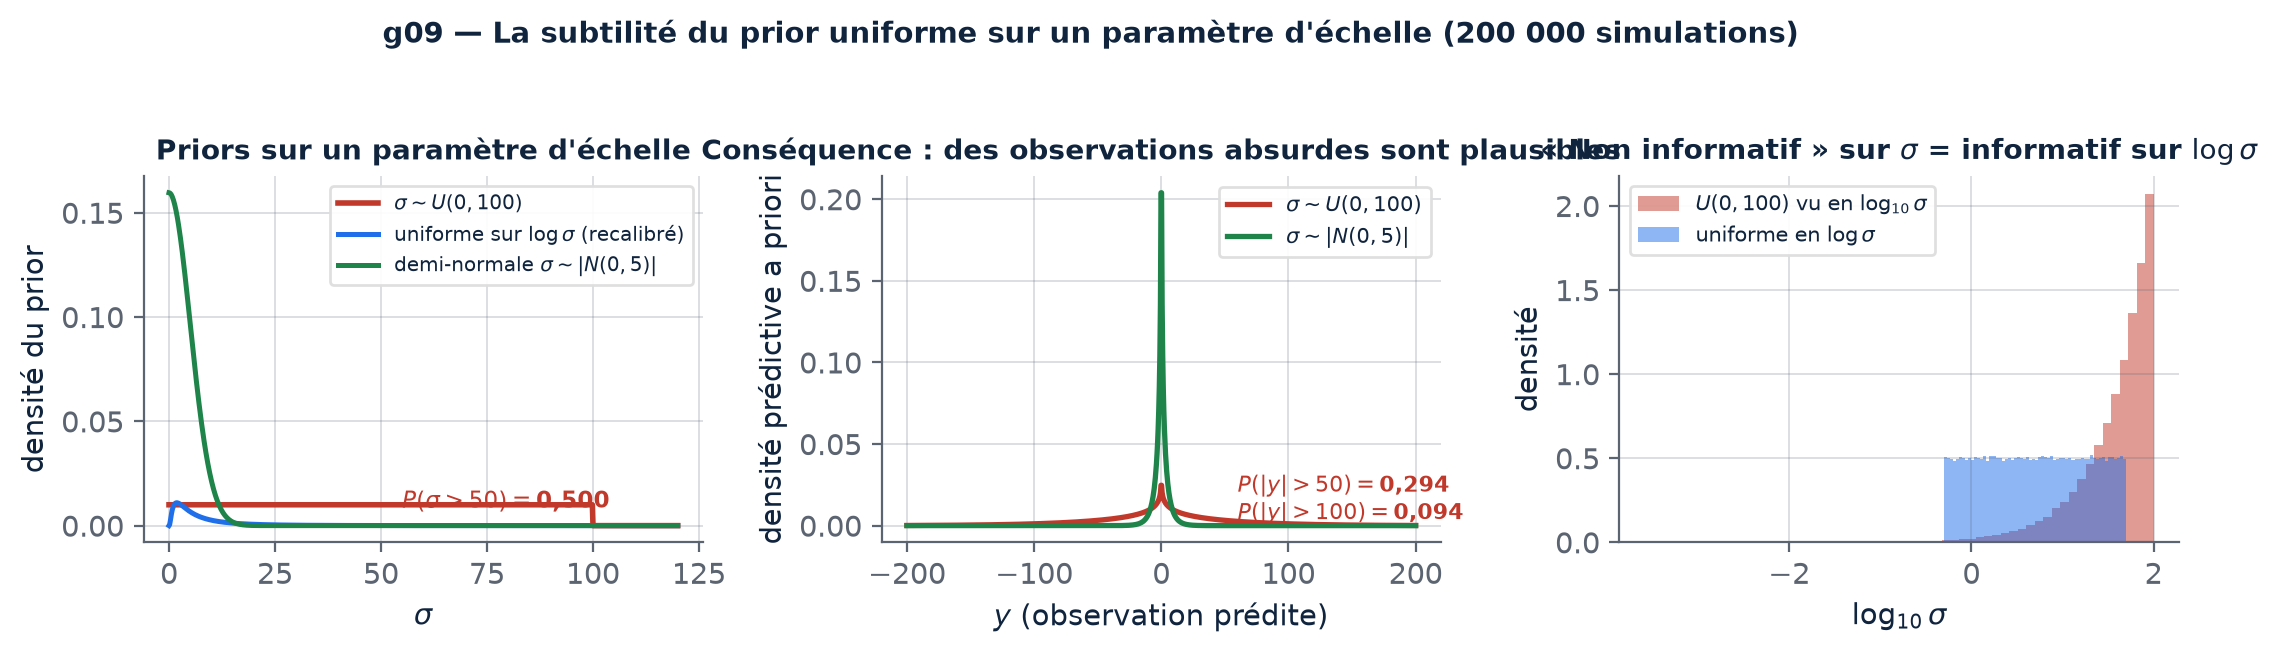
\includegraphics[width=.86\textwidth]{g09_uniforme_echelle.png}
\end{center}
\end{frame}

% [split]
% [suite]
\begin{frame}{La subtilité du prior uniforme sur un paramètre d'échelle}
\vspace{-1mm}
\begin{columns}[t]
\begin{column}{0.55\textwidth}
\begin{ebox}[Ce que disent les simulations]
Avec $\sigma \sim U(0, 100)$ (a priori « je n'en sais rien ») :
$P(\sigma > 50) = 0{,}500$ et la médiane de $\sigma$ vaut $50$.
Conséquence sur une observation $y \sim \N(0,\sigma)$ :
$P(|y| > 50) = 0{,}294$ et $P(|y| > 100) = 0{,}094$.
Un modèle de points SAT prédit donc des effets de $+100$ points comme
un événement banal.
\end{ebox}
\end{column}
\begin{column}{0.40\textwidth}
\begin{wbox}[L'erreur d'interprétation]
« Non informatif » sur $\sigma$ \textbf{devient très informatif} sur
$\log\sigma$ : la figure de droite montre la masse concentrée vers les grandes
valeurs. En informatique numérique on travaille presque toujours avec
$\log\sigma$ — donc un prior uniforme sur $\sigma$ n'est pas neutre du point
de vue de l'échelle, celui qui compte vraiment.
\end{wbox}
\end{column}
\end{columns}
\end{frame}

% [suite]
\begin{frame}{La subtilité du prior uniforme sur un paramètre d'échelle (suite)}
\begin{kbox}[La solution recommandée]
Un a priori uniforme sur $\log\sigma$, ou une demi-normale faiblement
informative (échelle fixée par la connaissance du phénomène), et
\textbf{toujours un contrôle prédictif a priori} avant de conclure.
\end{kbox}

\end{frame}

% ---------------------------------------------------------------- 7
% [suite]
\begin{frame}{L'a priori faiblement informatif : la voie raisonnable}
\begin{kbox}[Le principe de la standardisation]
Avant de choisir une échelle, on \textbf{standardise} : on exprime le paramètre en
unités de la variabilité du phénomène.
\[
z = \frac{y - \bar y}{s_y}, \qquad \text{puis } z \sim \N(0, 1) \text{ a priori}
\]
Le même prior marche alors pour des données en points SAT, en euros ou en secondes.
\end{kbox}
\vspace{1mm}
\begin{columns}[t]
\begin{column}{0.52\textwidth}
\begin{ebox}[Application aux 8 écoles]
Effets estimés en points SAT : moyenne $\mathbf{8{,}820}$,
écart-type $s_y = \mathbf{10{,}514}$, étendue $[-2{,}75 \,;\, 28{,}39]$,
erreur standard moyenne $12{,}650$.
Variables standardisées : $\mathbf{1{,}861}$, $\mathbf{-0{,}084}$,
$\mathbf{0{,}874}$, $\mathbf{0{,}318}$ pour les écoles A, B, G, H.
\end{ebox}
\end{column}
\begin{column}{0.45\textwidth}
\begin{ebox}[Traduire un dire d'expert]
« L'effet est faiblement positif, peut-être 10 points, sûrement pas
100 » se traduit par
$\mu \sim \N(10, 20^2)$, ou bien, en unités standardisées, $\mu \sim \N(0{,}5, 1^2)$ sur $z$.
puis on vérifie ce que ce prior prédit (section 2.3).
\end{ebox}
\end{column}
\end{columns}
\vspace{1mm}
\end{frame}

% [suite]
\begin{frame}{L'a priori faiblement informatif : la voie raisonnable (suite)}
\begin{wbox}[Pourquoi « faiblement informatif »]
Un prior faiblement informatif \textbf{régularise} les situations dégénérées
(une catégorie sans observation, une séparation parfaite en régression) tout en
laissant les données décider. C'est le réglage par défaut d'une analyse sérieuse.
\end{wbox}
\end{frame}

% ---------------------------------------------------------------- 8
\begin{frame}{Quiz 2 — choisir un a priori}
% [rogna]
\small
\begin{qbox}[Question 4 -- Classer et justifier]
\textbf{1.} Un capteur mesure un taux $\lambda$ de défauts par pièce. La chaîne
produit de 1 à 50 pièces par heure. Quel prior est préférable pour l'échelle :
$U(0, 100)$ sur $\lambda$, ou $U(\log \lambda)$, ou $\mathrm{Gamma}(1,1)$ ? \\[1mm]
\textbf{2.} Un collègue affirme : « j'ai mis $\mathrm{Beta}(1,1)$, donc mon
posterior est objectif ». Que répondez-vous ? \\[1mm]
\textbf{3.} Pour une proportion, $10$ essais antérieurs donnent $3$ succès.
Écrire un a priori faiblement informatif qui ne les ignore pas \emph{et} ne les
impose pas. \\[1mm]
\textbf{4.} Le tableau de la frame « boîte à outils » donne Beta$(0{,}5;0{,}5)$
comme impropre : comment est-ce possible pour la loi de Jeffreys de la
\emph{binomiale} ? \\[1mm]
\textbf{5.} Un paramètre d'échelle $\sigma$ est contraint physiquement :
$0 < \sigma < 200$. Quelle famille choisir, et laquelle éviter ?
\vspace{1.5mm}

\textcolor{byBlue}{\textbf{Éléments de réponse :}}
\textbf{1.} $U(\log\lambda)$ ou Gamma (invariance d'échelle) ;
un $U(0,100)$ donne la moitié de sa masse à $\lambda > 50$ : absurde.
\quad
\textbf{2.} Que l'uniforme \emph{n'est pas} invariant : il devient très informatif
après reparamétrisation.
\quad
\textbf{3.} Beta$(1+3a, 1+7a)$ avec $a = 0{,}5$ : Beta$(2{,}5; 4{,}5)$, soit un poids
de $50$ \% pour l'historique.
\quad
\textbf{4.} Impropre \emph{a priori}, propre \emph{a posteriori} : les observations
apportent la convergence.
\quad
\textbf{5.} Une demi-normale tronquée ou une log-uniforme ; éviter le mélange
uniforme sur $\sigma$ qui favorise les grandes valeurs.
\end{qbox}
\end{frame}

% ---------------------------------------------------------------- 9
% [suite]
\begin{frame}{Activité guidée — éliciter un a priori (10 min)}
% [rogna]
\small
\begin{abox}[Consigne, par binôme de rôles]
L'énoncé de l'expert : « \emph{Le taux de retour d'un produit est faible, autour de
2 \%, je dirais entre 0,5 \% et 5 \%. Je n'ai jamais vu plus de 10 \%.} »
\begin{enumerate}
  \item Proposer une loi a priori, justifier la famille et les hyperparamètres.
  \item Calculer $a+b$ et commenter le nombre d'observations virtuelles.
  \item Vérifier par un contrôle prédictif quel nombre de retours ce prior prédit
        sur une commande de $200$ pièces.
\end{enumerate}
\end{abox}
\vspace{1mm}
\end{frame}

% [suite]
\begin{frame}{Activité guidée — éliciter un a priori (10 min) (suite)}
\begin{columns}[t]
\begin{column}{0.54\textwidth}
\begin{solbox}[Une réponse parmi d'autres (calculée)]
$\mathrm{Beta}(a,b)$ centré en $0{,}02$ avec $P(p < 0{,}05) \approx 0{,}95$ :
Beta$(2, 98)$ — moyenne $0{,}0200$, $a+b = 100$ soit
\textbf{98 observations virtuelles}, IC 95 \% $[0{,}0025 \,;\, 0{,}0550]$,
et $P(p < 0{,}05) = 0{,}9613$.
Sur $200$ pièces, le contrôle prédictif (20\,000 simulations) donne en moyenne
$3{,}99$ retours, un intervalle à $90$ \% de $[0 \,;\, 11]$ et
$P(k > 20) = 0{,}0011$ : le prior n'annonce jamais de catastrophes.
\end{solbox}
\end{column}
\begin{column}{0.43\textwidth}
\begin{ebox}[Un bon exercice d'ingénierie]
\begin{itemize}
  \item On a transformé une phrase en \textbf{deux nombres vérifiables} ;
  \item l'expert peut \emph{réfuter} : « 98 observations virtuelles, c'est
        trop, je ne suis pas si sûr » ;
  \item le désaccord devient un paramètre ($a+b$), donc une analyse de sensibilité
        (section 2.4) plutôt qu'une discussion de couloir.
\end{itemize}
\end{ebox}
\end{column}
\end{columns}
\end{frame}

% ---------------------------------------------------------------- 10
% [suite]
\begin{frame}{2.3 — Simuler avant d'avoir des données}
\begin{kbox}[L'idée en une phrase]
Avant d'estimer quoi que ce soit, on \textbf{simule le monde que le modèle
promet} — paramètres tirés du prior, puis données tirées de la vraisemblance — et
on se demande : ces données ressemblent-elles à celles qu'on \emph{attend} ?
\end{kbox}
\vspace{1mm}
\begin{columns}[t]
\begin{column}{0.50\textwidth}
\begin{ebox}[Un examen du prior]
Un \emph{prior predictive check} (PPC) ne regarde jamais les observations réelles
pour ajuster : il vérifie que le \textbf{domaine de plausibilité} du modèle est
compatible avec la physique ou le bon sens. C'est l'étape qui aurait sauvé
des projets entiers de deep learning bayésien.
\end{ebox}
\end{column}
\begin{column}{0.47\textwidth}
\begin{abox}[À faire devant la classe (2 min)]
Reprendre l'énoncé de l'expert de la frame précédente : avant même de collecter
des données, combien de retours le modèle peut-il prédire sur 200 pièces ?
Si la réponse dépasse 40, le prior est intenable.
\end{abox}
\end{column}
\end{columns}
\vspace{1mm}
\end{frame}

% [suite]
\begin{frame}{2.3 — Simuler avant d'avoir des données (suite)}
\begin{tcolorbox}[colback=byCyan!8,colframe=byCyan,arc=2mm,width=.95\textwidth]
\small\centering
\textbf{Ordre de travail professionnel} : (1) écrire le modèle, (2) simuler le prior
prédictif, (3) corriger l'échelle, (4) seulement alors regarder les données,
(5) vérifier le posterior prédictif (chapitres 3 et 4).
\end{tcolorbox}
\end{frame}

% ---------------------------------------------------------------- 11
\begin{frame}{Le contrôle prédictif a priori, en quatre étapes}
\begin{ebox}[La loi prédictive a priori]
\[
p(\tilde y) = \int p(\tilde y \given \theta)\, p(\theta)\,\mathrm{d}\theta
\qquad \text{simulation : } \theta^{(s)} \sim p(\theta),\;\;
\tilde y^{(s)} \sim p(\tilde y \given \theta^{(s)})
\]
\begin{enumerate}
  \item \textbf{Tirer} $S$ valeurs du paramètre sous le prior
        ($S = 20\,000$ dans nos scripts, $4\,000$ en PyMC).
  \item \textbf{Propager} dans la vraisemblance : on obtient $S$ jeux de données simulés.
  \item \textbf{Résumer} : moyenne prédite, intervalle à 90 \%, probabilité d'événements impossibles.
  \item \textbf{Juger} : ce que le modèle promet est-il physiquement admissible ?
        Sinon, recommencer à l'étape 1 avec une échelle corrigée.
\end{enumerate}
\end{ebox}
\vspace{1mm}
\begin{kbox}[Ce que l'étape 4 ne doit jamais être]
Un test statistique automatique. Le jugement est \textbf{métier} : « une teneur en
sucre négative », « une probabilité de 1,0 », « un effet de 300 points SAT ».
Le graphique remplace le test.
\end{kbox}
\end{frame}

% ---------------------------------------------------------------- 12
% [rogna]
% [rogna]
% [rogna]
% [split]
\begin{frame}{Que prédit chaque a priori ? Le cas Challenger}
\begin{center}
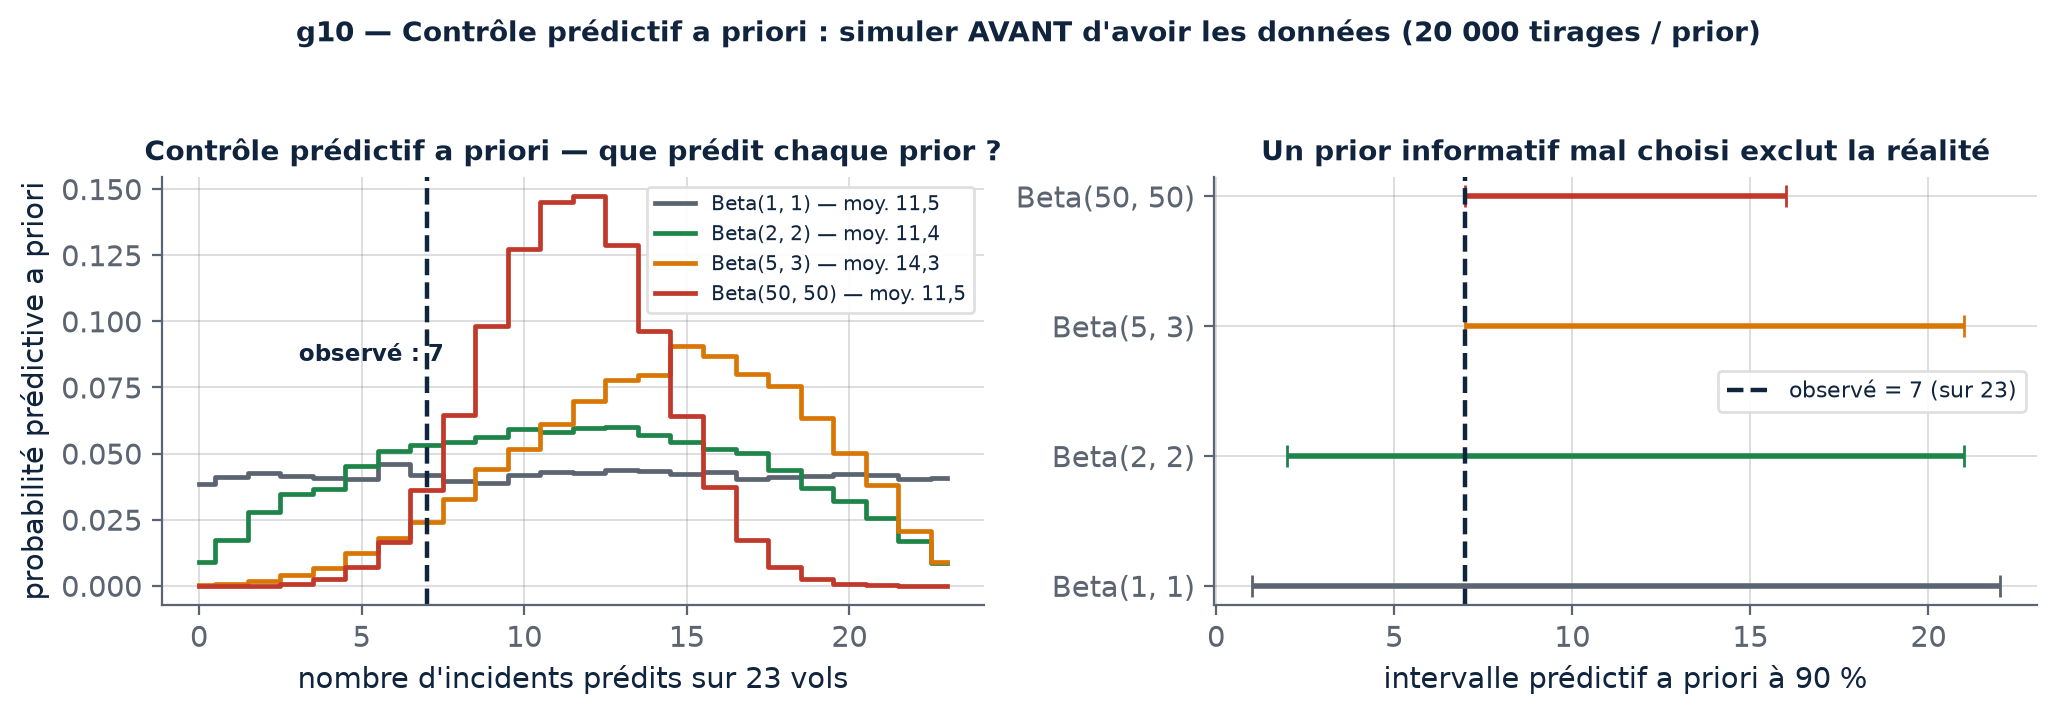
\includegraphics[width=.86\textwidth]{g10_prior_predictive.png}
\end{center}
\end{frame}

% [split]
\begin{frame}{Que prédit chaque a priori ? Le cas Challenger}

\vspace{-1mm}
\centering
\scriptsize\begin{tabular}{@{}lcccc@{}}
\toprule
\textbf{A priori} & \textbf{nombre prédit} & \textbf{intervalle 90 \%} &
$P(k \leq 7)$ & $P(p > 0{,}5)$ \\
\midrule
Beta$(1,1)$ & 11,52 & $[1 \,;\, 22]$ & $0{,}333$ & $0{,}499$ \\
Beta$(2,2)$ & 11,43 & $[2 \,;\, 21]$ & $0{,}275$ & $0{,}502$ \\
Beta$(5,3)$ & 14,35 & $[7 \,;\, 21]$ & $0{,}068$ & \textbf{0,769} \\
Beta$(50,50)$ & 11,51 & $[7 \,;\, 16]$ & $0{,}063$ & $0{,}504$ \\
\bottomrule
\end{tabular}
\vspace{1.5mm}

\begin{minipage}{.95\textwidth}
\begin{wbox}[Le verdict du contrôle]
Les valeurs réellement observées : $k = 7$ incidents sur $23$ vols.
Elle est 	extbf{parfaitement plausible} sous Beta$(1,1)$ (33	extsuperscript{e} percentile)
et 	extbf{très improbable} sous Beta$(5,3)$ et Beta$(50,50)$ (quantiles $0{,}068$ et
$0{,}063$). Conclusion : un prior centré sur 0,5 (le taux attendu d'une
pièce équilibrée) aurait \emph{exclu la réalité} — c'est exactement le diagnostic
que le PPC doit produire avant l'analyse.
\end{wbox}
\end{minipage}
\end{frame}

% ---------------------------------------------------------------- 13
% [rogna]
% [rogna]
% [rogna]
% [split]
\begin{frame}{Calibrer l'échelle : le cas d'école des huit écoles}
\begin{center}
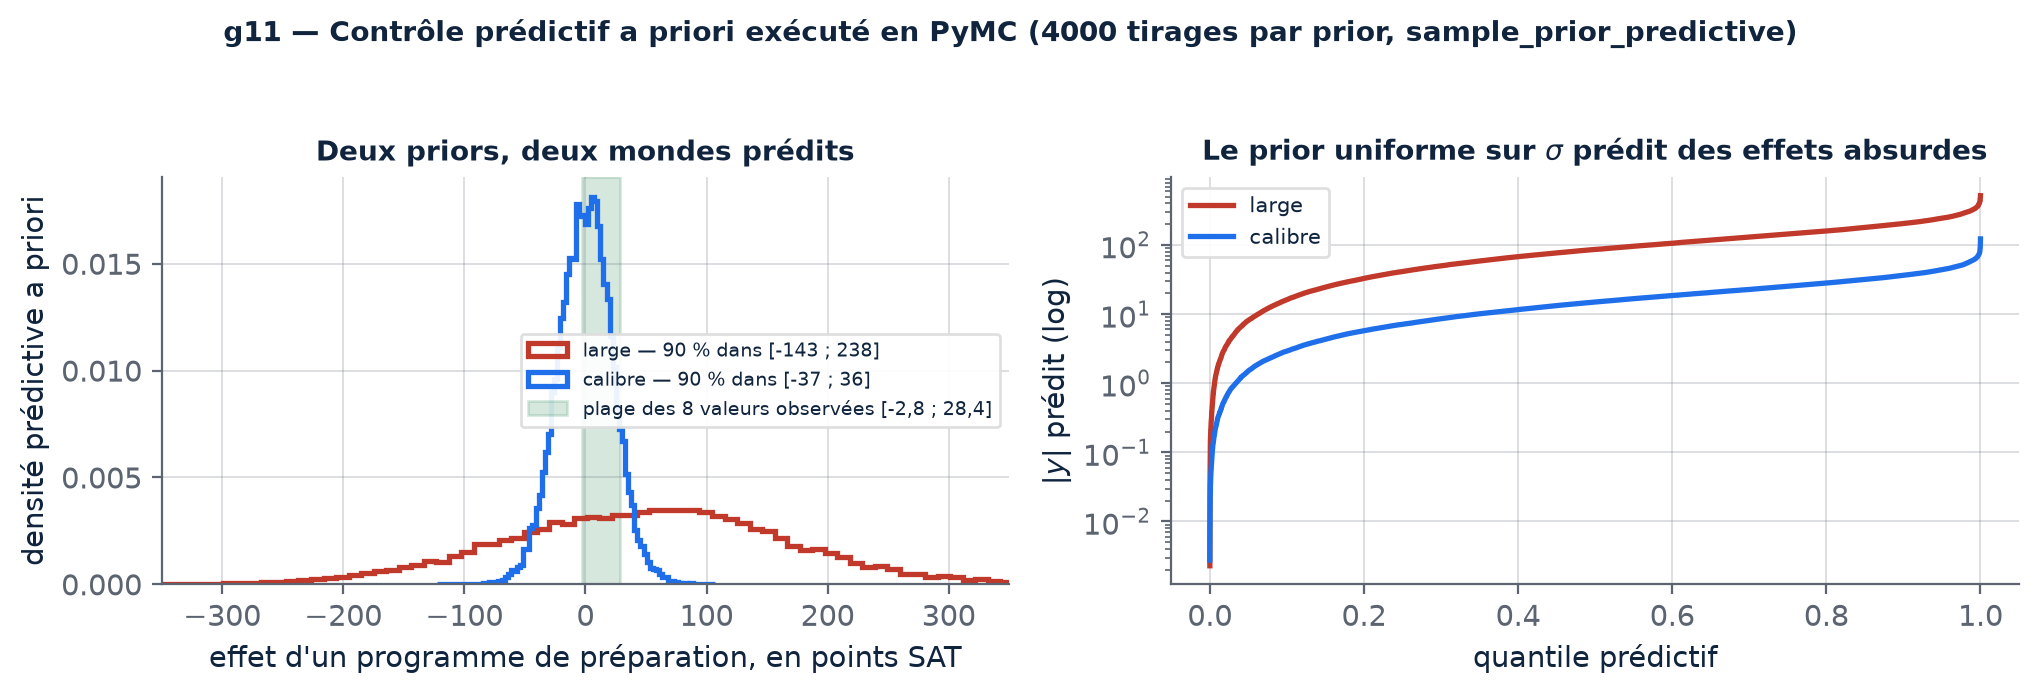
\includegraphics[width=.86\textwidth]{g11_prior_predictive_pymc.png}
\end{center}
\end{frame}

% [split]
\begin{frame}{Calibrer l'échelle : le cas d'école des huit écoles}

\vspace{-1mm}
\begin{columns}[t]
\begin{column}{0.55\textwidth}
\begin{ebox}[Deux priors exécutés en PyMC]
Effets attendus d'un programme SAT, en points ; les valeurs observées vivent
dans $[-2{,}75 \,;\, 28{,}39]$.
\begin{itemize}
  \item prior \textbf{calibré} : $\mu \sim \N(0, 20^2)$, $\sigma \sim \mathrm{HN}(10)$
        $\Rightarrow$ 90 \% des effets prédits dans $[-37{,}0 \,;\, 36{,}0]$ points, et
        seulement $0{,}02$ \% des cas au-delà de $\pm 100$ points : compatible avec la réalité ;
  \item prior \textbf{large} : $\mu \sim \N(50, 100^2)$, $\sigma \sim U(0,100)$
        $\Rightarrow$ 90 \% des effets dans $[-142{,}7 \,;\, 238{,}2]$, amplitudes
        de $\pm 324{,}9$ points au 99\textsuperscript{e} percentile et
        $P(|y| > 100) = \mathbf{0{,}430}$ : quatre effets prédits sur dix sont
        absurdes pour un test scolaire.
\end{itemize}
\end{ebox}
\end{column}
\begin{column}{0.42\textwidth}
\begin{kbox}[Le réflexe]
Le contrôle prédictif a priori ne sert pas à \emph{choisir} entre deux théories :
il sert à \textbf{éliminer les échelles impossibles}, puis à retenir une échelle
faiblement informative qui laisse les données décider.
\end{kbox}
\end{column}
\end{columns}
\end{frame}

% ---------------------------------------------------------------- 14
% [suite5]
\begin{frame}[fragile]{La ligne de code qui change une analyse}
\begin{columns}[t]
\begin{column}{0.54\textwidth}
\begin{codebox}[src/fig\_ch2b\_pymc.py — PPC sur le modèle des 8 écoles]
\begin{lstlisting}
y = np.array([28.39, 7.94, -2.75, 6.82,
              -0.64, 0.63, 18.01, 12.16])

with pm.Model() as m:
    mu = pm.Normal("mu", mu=0, sigma=20)     # calibre
    sigma = pm.HalfNormal("sigma", 10)
    pm.Normal("y", mu=mu, sigma=sigma, shape=8)

    # 4000 mondes possibles AVANT toute donnee
    prior = pm.sample_prior_predictive(draws=4000,
                                       random_seed=42)

ypred = prior.prior["y"].values.reshape(-1, 8)
print(np.percentile(ypred, [5, 50, 95]))
print((np.abs(ypred) > 100).mean())

# puis seulement : pm.sample() pour le posterior
\end{lstlisting}
\end{codebox}
\end{column}
\begin{column}{0.43\textwidth}
\begin{kbox}[Trois bonnes pratiques de code]
\begin{itemize}
  \item Un \textbf{script par question} : le PPC dans le fichier du modèle ;
  \item une \py{random_seed} fixée : un contrôle doit être reproductible ;
  \item sauvegarder les chiffres (ici \file{figures/key\_numbers\_ch2.json})
        pour que les slides citent des valeurs exécutées.
\end{itemize}
\end{kbox}
\end{column}
\end{columns}
\end{frame}

% [suite5]
\begin{frame}{La ligne de code qui change une analyse (suite)}
\begin{wbox}[Le piège de la relecture]
\py{sample_prior_predictive} place ses tirages dans le groupe \py{prior} de
l'objet ArviZ (et non dans \py{prior_predictive}) : vérifier le nom du groupe
— c'est l'erreur qui a réellement interrompu ce script à la première exécution.
\end{wbox}
\end{frame}

% ---------------------------------------------------------------- 15
\begin{frame}{Du contrôle a priori au contrôle a posteriori}
\begin{columns}[t]
\begin{column}{0.49\textwidth}
\begin{kbox}[Prior predictive check (PPC)]
\begin{itemize}
  \item \textbf{Quand} : avant de voir les données.
  \item \textbf{Distribution} : $p(\tilde y) = \int p(\tilde y \given \theta)p(\theta)\mathrm{d}\theta$.
  \item \textbf{Question} : le modèle prédit-il un monde possible ?
  \item \textbf{Décision} : corriger l'échelle du prior.
\end{itemize}
\end{kbox}
\end{column}
\begin{column}{0.49\textwidth}
\begin{kbox}[Posterior predictive check (PPC$'$)]
\begin{itemize}
  \item \textbf{Quand} : après l'inférence.
  \item \textbf{Distribution} : $p(\tilde y \given y) = \int p(\tilde y \given \theta)p(\theta \given y)\mathrm{d}\theta$.
  \item \textbf{Question} : le modèle \emph{ajusté} reproduit-il les données ?
  \item \textbf{Décision} : revoir le modèle (chapitres 3 et 4).
\end{itemize}
\end{kbox}
\end{column}
\end{columns}
\vspace{1mm}
\begin{ebox}[Les deux contrôles de ce cours]
Sur Challenger, le contrôle a priori compare les 4 priors du paragraphe précédent
(bonnes échelles) ; sur les 8 écoles, le contrôle a posteriori du chapitre 3 vérifie
que les effets simulés couvrent bien les 8 effets observés. Un modèle qui passe les
deux est un modèle \textbf{crédible}, pas seulement convergé.
\end{ebox}
\end{frame}

% ---------------------------------------------------------------- 16
\begin{frame}{Pièges du contrôle prédictif}
\begin{qbox}[Question 5 -- Le PPC trompeur]
Un étudiant annonce : « mon PPC est parfait : les données simulées couvrent exactement
les données observées ».
\vspace{1mm}

\textbf{a)} Qu'a-t-il probablement fait de mal ? \\[1mm]
\textbf{b)} Peut-on \emph{valider} un modèle avec un PPC ? \\[1mm]
\textbf{c)} Un prior tellement large que tout est prédit doit-il être préféré ?
\vspace{1.5mm}

\textcolor{byBlue}{\textbf{Réponses :}}
\textbf{a)} Un prior trop large prédit tout : la couverture ne coûte rien.
Il faut regarder aussi la \emph{concentration} des prédictions
(ici, un intervalle à 90 \% de 22 valeurs pour $n=23$ ne discrimine rien).
\quad
\textbf{b)} Non : un PPC ne \emph{falsifie} que des modèles grossièrement faux ;
il n'établit jamais la vérité d'un modèle — seule la prévision hors échantillon
répond à cette question.
\quad
\textbf{c)} Non : un prior qui prédit un taux d'incident de 95 \% est plus
« couvrant » et pourtant inutilisable ; le but est la \emph{calibration}, pas la
largeur.
\end{qbox}
\end{frame}

% ---------------------------------------------------------------- 17
\begin{frame}{Synthèse 2.2 et 2.3 — choisir et tester son a priori}
% [rogna]
\small
\begin{kbox}[Six règles issues de la pratique]
\begin{enumerate}
  \item Écrire le prior en \textbf{taille d'échantillon virtuelle} ($a+b$, $n_0$) et
        le dire à voix haute.
  \item Préférer un a priori \textbf{faiblement informatif} sur une échelle
        standardisée ; réserver le non informatif à un objectif d'invariance
        affiché.
  \item Sur un paramètre d'échelle, \textbf{jamais} d'uniforme sur $\sigma$ :
        travailler sur $\log\sigma$ ou avec une demi-normale calibrée.
  \item Vérifier la \textbf{propreté} du posterior quand le prior est impropre.
  \item Faire un \textbf{contrôle prédictif a priori} et savoir citer au moins un
        événement prédit impossible.
  \item Documenter : modèle, prior, échelle, contrôle — dans le rapport, pas dans
        les commentaires du code.
\end{enumerate}
\end{kbox}
\vspace{-2mm}
\begin{columns}[t]
\begin{column}{0.55\textwidth}
\begin{ebox}[Transition vers 2.4]
Il reste la question la plus redoutée : « et si je change d'avis sur le prior ? »
La section suivante quantifie la \textbf{sensibilité} et la rend mesurable.
\end{ebox}
\end{column}
\begin{column}{0.42\textwidth}
\begin{wbox}[Les trois chiffres à retenir]
Beta$(50,50)$ face à 23 données : $w = 0{,}813$ \; ; \; uniforme sur $\sigma$ :
$P(|y| > 100) = 0{,}094$ \; ; \; Beta$(5,3)$ exclut la réalité observée au seuil de
$7$ \%.
\end{wbox}
\end{column}
\end{columns}
\end{frame}

% =====================================================================
%  EPD-SDIA-4112 -- Statistique Bayesienne -- Master 1 SDIA
%  CHAPITRE 2 : Distributions a priori et a posteriori
%  Fichier C : sections 2.4 (robustesse, sensibilite, shrinkage) et 2.5 (synthese)
% =====================================================================

% ---------------------------------------------------------------- 1
% [suite]
\begin{frame}{2.4 — « Et si mon a priori est faux ? »}
% [rogna]
\small
\begin{kbox}[Trois questions, trois réponses]
\begin{enumerate}
  \item \textbf{À quelle vitesse} les données prennent-elles le dessus ?
        Réponse : l'information s'accumule en $1/\sqrt{n}$, le décalage du prior
        décroît en $1/n$.
  \item \textbf{Combien de poids} donner à un historique ? Réponse : le
        \emph{power prior}, un curseur $a_0 \in [0,1]$ à justifier.
  \item \textbf{Que faire de plusieurs groupes} quand certains sont petits ?
        Réponse : un prior hiérarchique, c'est-à-dire du \emph{shrinkage}.
\end{enumerate}
\end{kbox}
\vspace{1mm}
\end{frame}

% [suite]
\begin{frame}{2.4 — « Et si mon a priori est faux ? » (suite)}
\begin{columns}[t]
\begin{column}{0.55\textwidth}
\begin{ebox}[Le cadre : sensibilité]
On ne cherche plus « le bon prior » (il n'existe pas) mais \textbf{l'effet du choix
de prior}. Sur une proportion $p$ réellement égale à $0{,}35$, avec un
$\mathrm{Beta}(50,50)$ (centré sur $0{,}5$, donc \emph{faux}) :
\begin{center}
\begin{tabular}{@{}lcccc@{}}
\toprule
\textbf{Prior} & $n = 10$ & $n = 100$ & $n = 1000$ & $n = 3000$ \\
\midrule
Beta$(1,1)$   & 0,4167 & 0,3627 & 0,3303 & 0,3441 \\
Beta$(2,2)$   & 0,4286 & 0,3654 & 0,3307 & 0,3442 \\
Beta$(5,3)$   & 0,5000 & 0,3796 & 0,3323 & 0,3447 \\
Beta$(50,50)$ & 0,4909 & 0,4300 & 0,3455 & 0,3490 \\
\bottomrule
\end{tabular}
\end{center}
\hfill\footnotesize moyenne a posteriori ($p$ vrai $= 0{,}35$)
\end{ebox}
\end{column}
\begin{column}{0.42\textwidth}
\begin{wbox}[Lecture honnête du tableau]
À $n = 10$, le prior \emph{faux} déplace la réponse de $0{,}15$ (0,49 contre 0,35) :
la conclusion est pilotée par le prior. À $n = 3000$, tous les priors se recollent
autour de $0{,}34$–$0{,}35$ : \textbf{les données gagnent, mais lentement} et sans
jamais effacer complètement le décalage (voir frame suivante).
\end{wbox}
\end{column}
\end{columns}
\end{frame}

% ---------------------------------------------------------------- 2
% [rogna]
% [rogna]
\begin{frame}{La vitesse de dominance des données}
\begin{center}
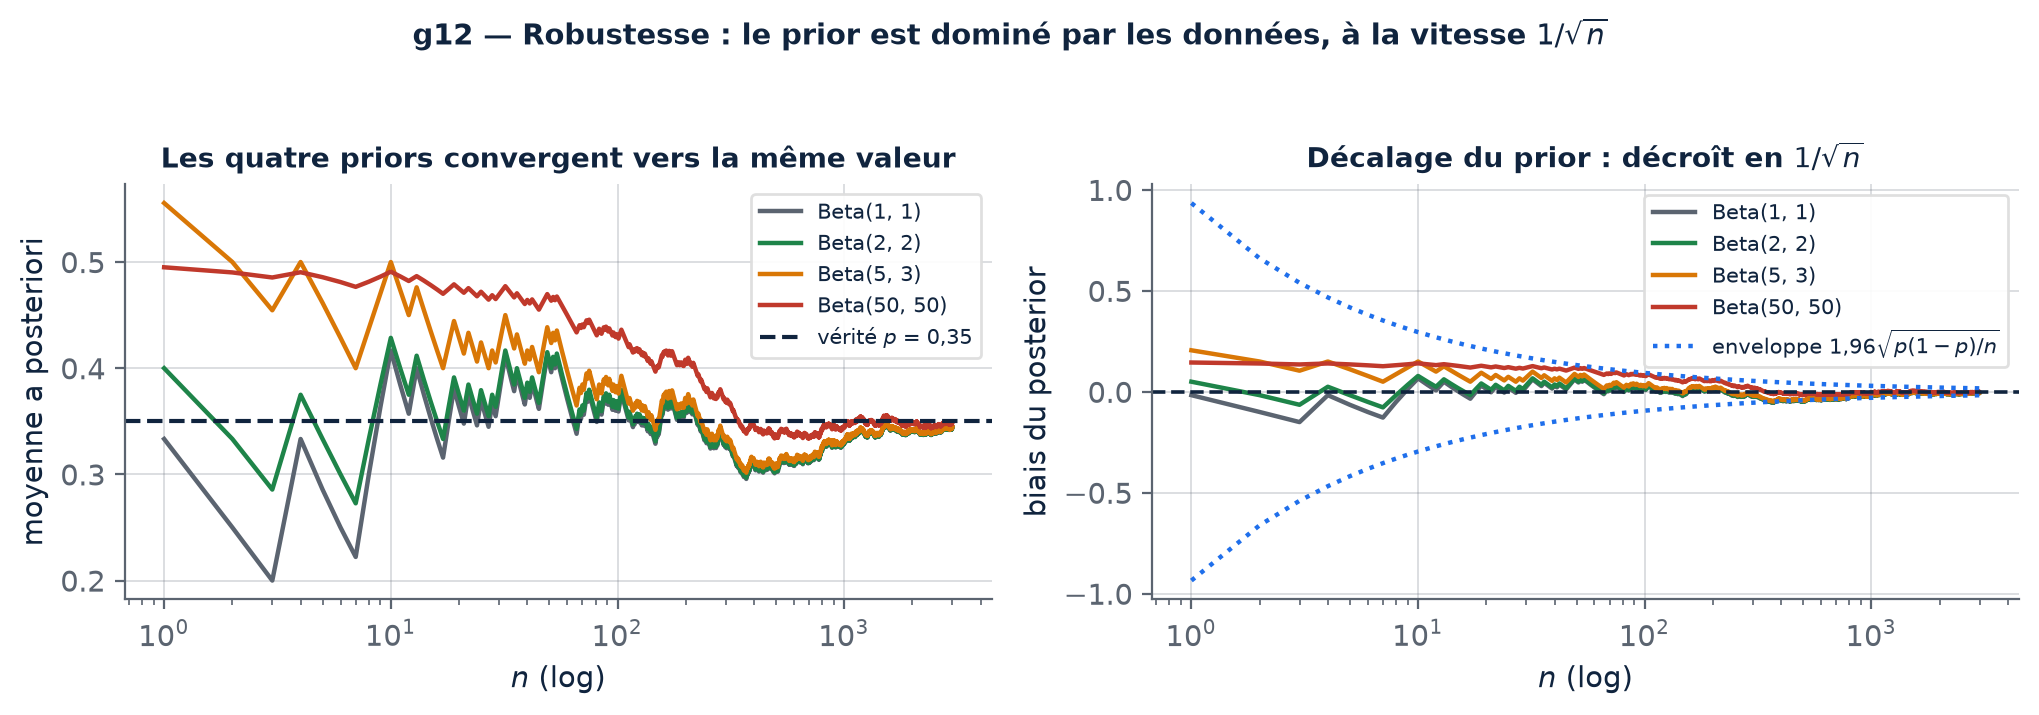
\includegraphics[width=0.72\textwidth]{g12_sensibilite_n.png}
\end{center}
\vspace{-1mm}
\begin{columns}[t]
\begin{column}{0.53\textwidth}
\begin{ebox}[Ce que mesurent les courbes]
L'écart-type de la loi des données vaut $\sqrt{p(1-p)/n}$ et suit exactement
la loi $1/\sqrt{n}$ : $0{,}1508$ pour $n = 10$, $0{,}0477$ pour $n = 100$,
$0{,}0151$ pour $n = 1000$, $0{,}0087$ pour $n = 3000$
(rapport $0{,}1508/0{,}0087 = 17{,}3 = \sqrt{300}$).
\end{ebox}
\end{column}
\begin{column}{0.44\textwidth}
\begin{kbox}[La bonne façon de le dire]
Le posterior se resserre comme $1/\sqrt{n}$, mais la \emph{position} de son centre
n'est pas garantie : c'est le décalage résiduel du prior, qui décroît seulement
en $1/n$ (frame suivante). Retenir la phrase : \textbf{la précision s'achète en
$1/\sqrt{n}$, la robustesse au prior s'achète en $1/n$}.
\end{kbox}
\end{column}
\end{columns}
\end{frame}

% ---------------------------------------------------------------- 3
\begin{frame}{Deux vitesses différentes : le résultat qui surprend}
\begin{columns}[t]
\begin{column}{0.56\textwidth}
\begin{ebox}[Décomposition exacte du biais]
\[
\text{biais} = \frac{(a+b)\,(m_{\post} - p)}{a+b+n} = \frac{15}{100+n},
\qquad
\text{sd} \approx \sqrt{\frac{p(1-p)}{n}}
\]
\begin{center}
\begin{tabular}{@{}lcccc@{}}
\toprule
$n$ & \textbf{biais du prior} & \textbf{sd du posterior} & \textbf{rapport} &
\textbf{poids } $w$ \\
\midrule
10   & 0,1364 & 0,0474 & \textbf{2,87} & 0,9091 \\
100  & 0,0750 & 0,0349 & 2,15 & 0,5000 \\
1000 & 0,0136 & 0,0145 & 0,94 & 0,0909 \\
3000 & 0,0048 & 0,0086 & \textbf{0,56} & 0,0323 \\
\bottomrule
\end{tabular}
\end{center}
\end{ebox}
\end{column}
\begin{column}{0.41\textwidth}
\begin{kbox}[La conséquence contre-intuitive]
Quand $n$ grandit, l'\textbf{incertitude} du posterior diminue plus vite que le
\textbf{décalage} dû au prior : le rapport passe de $2{,}87$ (le biais écrase tout)
à $0{,}56$ (l'incertitude devient plus petite que le biais résiduel).
Autrement dit : \emph{plus on a de données, plus un prior mal calibré est
dangereux}, car il n'apparaît plus dans l'intervalle de crédibilité.
\end{kbox}
\begin{ebox}[Le garde-fou]
Toujours faire l'analyse de sensibilité \textbf{à $n$ grand}, pas à $n$ petit :
c'est là que le biais du prior se cache.
\end{ebox}
\end{column}
\end{columns}
\end{frame}

% ---------------------------------------------------------------- 4
% [rogna]
% [rogna]
% [rogna]
\begin{frame}{Power prior : régler le poids du passé}
\begin{center}
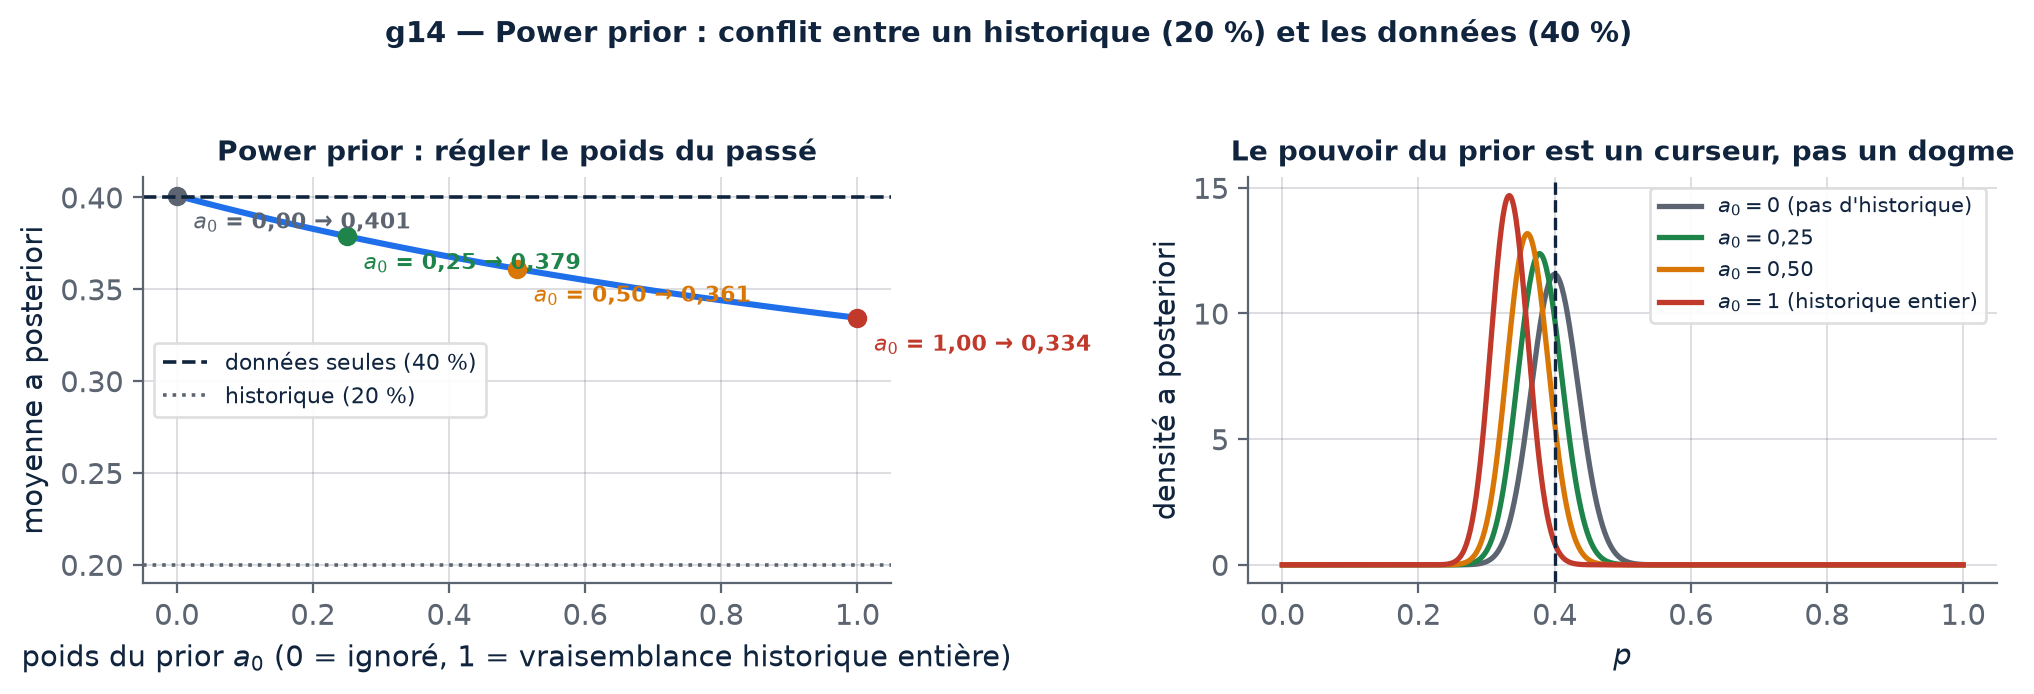
\includegraphics[width=.88\textwidth]{g14_power_prior.png}
\end{center}
\end{frame}

\begin{frame}{Power prior : régler le poids du passé --- le curseur $a_0$}
\begin{columns}[t]
\begin{column}{0.48\textwidth}
\begin{ebox}[La situation classique de conflit]
\begin{itemize}
  \item \textbf{Historique} : $20$ succès sur $100$ essais $(p_0 = 0{,}20)$ ;
  \item \textbf{Étude actuelle} : $80$ succès sur $200$ essais $(p_1 = 0{,}40)$.
\end{itemize}
Le passé contredit le présent : un prior informatif « normal » imposerait
$0{,}20$ à des données qui disent $0{,}40$.
\end{ebox}
\end{column}
\begin{column}{0.48\textwidth}
\begin{solbox}[Le curseur $a_0$ (calculs exécutés)]
$p(\theta) \propto p(\theta \given \data_0)^{a_0}$ donne
\[
\begin{aligned}
\mathrm{Beta}\bigl(&a_0 s_0 + s_1 + 1,\\
&a_0 (n_0 - s_0) + (n_1 - s_1) + 1\bigr)
\end{aligned}
\]
\begin{center}
\resizebox{\ifdim\width>\linewidth\linewidth\else\width\fi}{!}{%
\begin{tabular}{@{}lcc@{}}
\toprule
$a_0$ & \textbf{moyenne post.} & \textbf{IC 95 \%} \\
\midrule
0 (ignoré) & 0,4010 & $[0{,}3346;0{,}4693]$ \\
0,25 & 0,3789 & --- \\
0,50 & 0,3611 & --- \\
1 (entier) & 0,3344 & $[0{,}2824;0{,}3886]$ \\
\bottomrule
\end{tabular}}
\end{center}
\end{solbox}
\end{column}
\end{columns}
\vspace{1mm}
\centering\small
\textbf{Morale} — le désaccord entre passé et présent se transforme en
\emph{paramètre} $a_0$ : le rapport d'analyse peut alors discuter, chiffre en main,
du poids à donner à l'historique.
\end{frame}

% ---------------------------------------------------------------- 5
\begin{frame}[fragile]{Prior hiérarchique : le pooling partiel}
% [rogna]
\footnotesize
\begin{columns}[t]
\begin{column}{0.54\textwidth}
\begin{codebox}[src/fig\_ch2b\_pymc.py — modèle hiérarchique non centré]
\begin{lstlisting}
se = np.array([14.9, 10.2, 16.3, 11.0,
               9.4, 11.4, 10.4, 17.6])   # erreurs types

with pm.Model() as m_h:
    mu  = pm.Normal("mu", 0, 25)          # moyenne pop.
    tau = pm.HalfNormal("tau", 10)        # dispersion inter-groupes
    z   = pm.Normal("z", 0, 1, shape=8)   # N(0,1) "centree"
    theta = pm.Deterministic("theta", mu + tau * z)
    pm.Normal("y", mu=theta, sigma=se, observed=y)

    idata = pm.sample(draws=2000, tune=1500,
                      chains=2, cores=1,
                      target_accept=0.9)
\end{lstlisting}
\end{codebox}
\end{column}
\begin{column}{0.43\textwidth}
\begin{kbox}[Théorie : trois régimes]
\[
\theta_j \sim \N(\mu, \tau^2), \qquad y_j \sim \N(\theta_j, se_j^2)
\]
\begin{itemize}
  \item $\tau \to \infty$ : \textbf{pas de pooling} — chaque groupe estimé seul ;
  \item $\tau \to 0$ : \textbf{pooling total} — un seul effet pour tous ;
  \item $\tau$ estimé : \textbf{pooling partiel} — c'est le modèle hiérarchique.
\end{itemize}
\end{kbox}
\begin{wbox}[Pourquoi la forme « non centrée »]
Écrire $\theta_j = \mu + \tau z_j$ avec $z_j \sim \N(0,1)$ évite le \emph{funnel}
(entonnoir $\mu$--$\tau$--$\theta$) qui fait diverger NUTS quand $\tau$ est petit :
même modèle, géométrie numérique différente.
\end{wbox}
\end{column}
\end{columns}
\end{frame}

% ---------------------------------------------------------------- 6
% [rogna]
% [rogna]
% [rogna]
% [split]
\begin{frame}{Shrinkage : les huit écoles se rapprochent de la moyenne}
\begin{center}
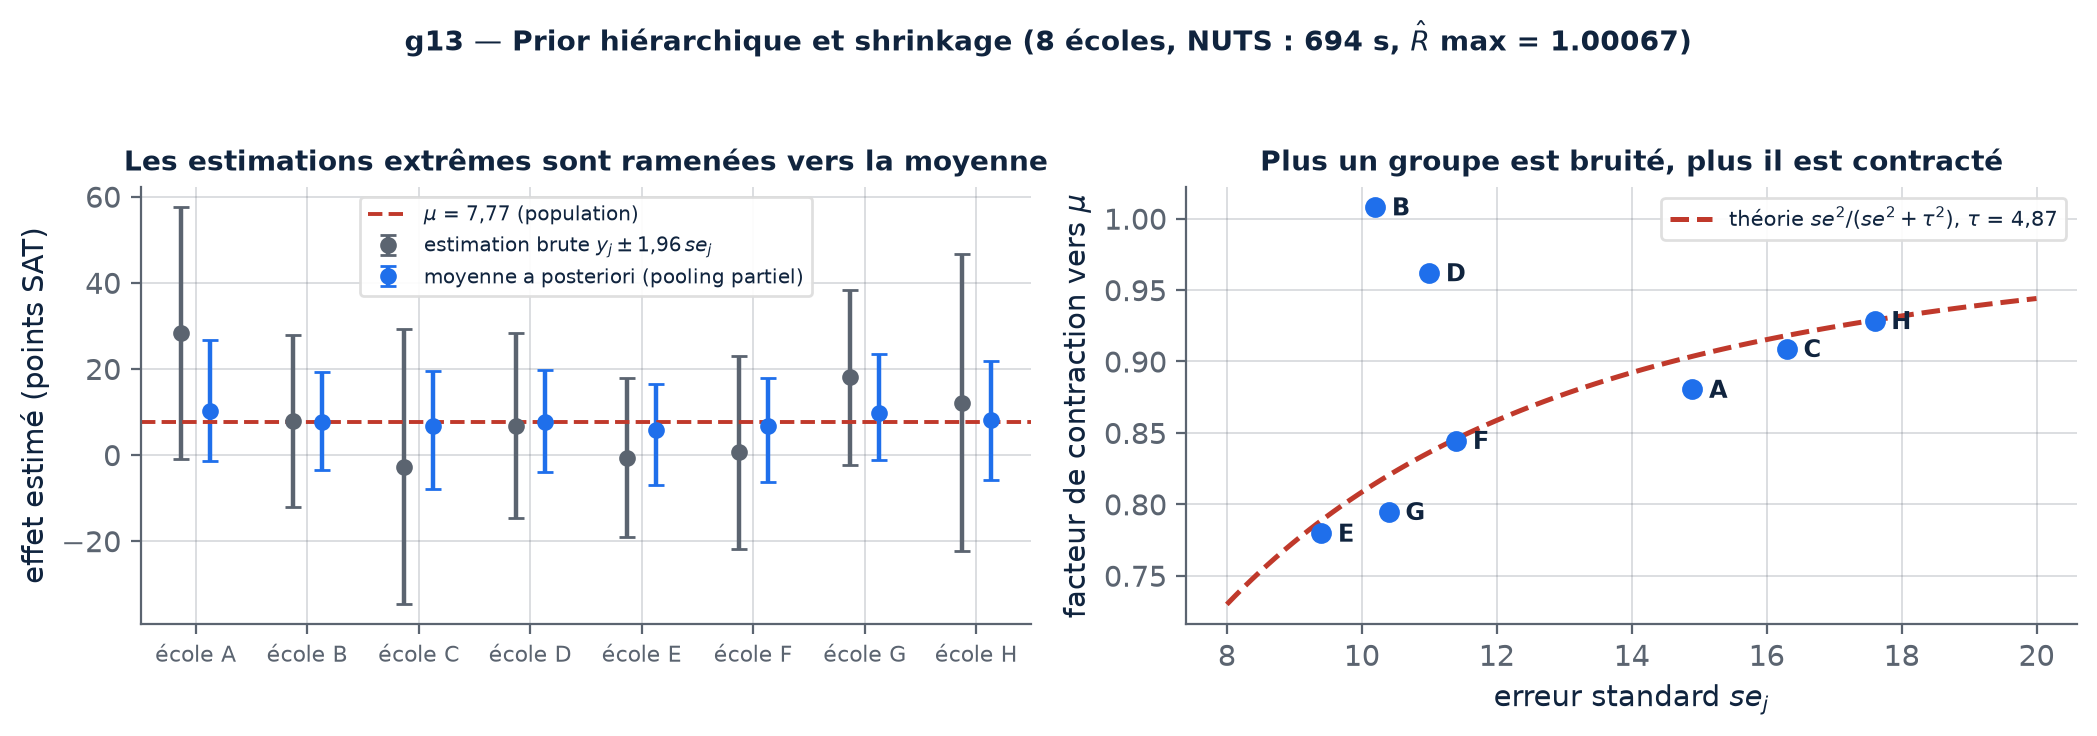
\includegraphics[width=.86\textwidth]{g13_shrinkage_8groupes.png}
\end{center}
\end{frame}

% [split]
\begin{frame}{Shrinkage : les huit écoles se rapprochent de la moyenne}

\vspace{-1mm}
\begin{columns}[t]
\begin{column}{0.55\textwidth}
\begin{ebox}[Résultats NUTS sur CPU]
$\mu = 7{,}766$, IC 95 \% $[-1{,}230 \,;\, 16{,}576]$ \;;\;
$\tau = 4{,}867$, IC 95 \% $[0{,}193 \,;\, 13{,}970]$ \; ;\;
$\hat R < 1{,}001$, ESS $> 2\,143$.
\end{ebox}
\begin{tabular}{@{}lcccccc@{}}
\toprule
\textbf{École} & A & B & C & D & E & G \\
\midrule
brut $y_j$ & 28,39 & 7,94 & $-2{,}75$ & 6,82 & $-0{,}64$ & 18,01 \\
posterior & 10,23 & 7,77 & 6,81 & 7,73 & 5,91 & 9,87 \\
contraction & 0,880 & 1,008 & 0,909 & 0,962 & 0,780 & 0,795 \\
\bottomrule
\end{tabular}
\end{column}
\begin{column}{0.42\textwidth}
\begin{kbox}[Le mécanisme, chiffré]
Largeur moyenne d'un intervalle : \textbf{49,59} points avec les données seules,
\textbf{25,27} avec le modèle hiérarchique, soit $-49$ \%. École H
($se = 17{,}6$) : contraction $0{,}929 = se^2/(se^2+\tau^2)$, exactement la
valeur théorique.
\end{kbox}
\begin{wbox}[Le piège du ratio par groupe]
Pour l'école B, dont l'estimation brute est \emph{déjà} proche de $\mu$, le ratio
observé vaut $1{,}008$ (supérieur à 1) : le ratio par groupe est instable quand
$y_j \approx \mu$. \textbf{Comparer les largeurs d'intervalles}, pas les ratios.
\end{wbox}
\end{column}
\end{columns}
\end{frame}

% ---------------------------------------------------------------- 7
\begin{frame}{Pourquoi le shrinkage est une bonne nouvelle}
% [rogna]
\small
\begin{columns}[t]
\begin{column}{0.49\textwidth}
\begin{kbox}[Compromis biais-variance]
Contracter une estimation vers une moyenne commune \textbf{introduit un biais}
(la vraie valeur d'un groupe n'est pas $\mu$) mais \textbf{réduit fortement la
variance}, parce qu'un groupe à $se$ élevé fournit peu d'information.
Le posterior tranche automatiquement en fonction de $se_j$ : c'est l'estimation
\emph{optimale} au sens de l'erreur quadratique attendue, exactement comme une
régression ridge (à cette différence que le coefficient de contraction $\tau$
est \emph{estimé} au lieu d'être réglé à la main).
\end{kbox}
\begin{ebox}[Test empirique simple]
Le modèle hiérarchique prédit un nouvel essai plus précisément que les
$8$ estimations brutes : c'est le critère qui compte, non la fidélité aux données.
\end{ebox}
\vspace{-3mm}
\end{column}
\begin{column}{0.48\textwidth}
\begin{abox}[Activité -- 10 min en binôme]
\begin{enumerate}
  \item Rejouer le modèle avec $\tau$ fixé à $0{,}1$ puis à $100$ : que
        deviennent les estimations ?
  \item Comparer à un modèle \emph{non} hiérarchique ($\theta_j$ estimés
        indépendamment, prior $\N(0,100^2)$) : qui gagne en largeur d'intervalle ?
  \item Conclure : que fait réellement l'a priori hiérarchique que ne fait
        aucun prior plat ?
\end{enumerate}
\end{abox}
\begin{solbox}[La réponse en une phrase]
Le prior hiérarchique \textbf{emprunte de l'information entre groupes} : c'est le
seul dispositif qui améliore un groupe en regardant les autres, tout en laissant
$\tau$ décider de la quantité d'emprunt.
\end{solbox}
\end{column}
\end{columns}
\end{frame}

% ---------------------------------------------------------------- 8
\begin{frame}{Quiz 3 — robustesse et shrinkage}
\begin{qbox}[Question 6 -- Quantifier la sensibilité]
\textbf{1.} Un prior $p \sim \mathrm{Beta}(50,50)$ est utilisé avec $n = 3000$
observations. Le biais potentiel du prior est-il dans l'intervalle de crédibilité ?
Conclure sur la sécurité de l'analyse. \\[1mm]
\textbf{2.} Vous avez $n = 12$ par groupe et $8$ groupes. Pourquoi un modèle
hiérarchique est-il préférable à huit estimations séparées ? \\[1mm]
\textbf{3.} Un collègue propose un power prior $a_0 = 1$ avec un historique
de $10\,000$ patients. Quel est l'effet sur $w$ ? \\[1mm]
\textbf{4.} Que signifie un posterior $\tau$ dont l'IC 95 \% est
$[0{,}193 \,;\, 13{,}970]$ ? \\[1mm]
\textbf{5.} Le shrinkage peut-il créer un biais \emph{plus grand} que le biais
du prior plat ? Dans quel cas ?
\vspace{1.5mm}

\textcolor{byBlue}{\textbf{Éléments de réponse :}}
\textbf{1.} Biais $= 15/(100+3000) = 0{,}0048$ contre une sd de $0{,}0086$ :
\textbf{non}, il n'est pas visible, et c'est précisément le danger.
\quad
\textbf{2.} L'information inter-groupes remplace l'absence de données (ici
$12$ observations par groupe) ; $\tau$ est estimé, donc l'emprunt est contrôlé.
\quad
\textbf{3.} $10\,000$ patients historiques écrasent l'étude actuelle :
$w \approx 10\,000/(10\,000+n) \approx 1$ — c'est un dogme, pas un prior.
\quad
\textbf{4.} Beaucoup d'incertitude sur l'hétérogénéité : les deux extrêmes
(pooling total et absence de pooling) restent crédibles ; il faut des données
pour trancher, ou un prior faiblement informatif sur $\tau$.
\quad
\textbf{5.} Oui, si $\tau$ est forcé trop petit alors que les groupes diffèrent
réellement : on écrase une hétérogénéité réelle (sous-dispersion).
\end{qbox}
\end{frame}

% ---------------------------------------------------------------- 9
% [suite]
\begin{frame}{Pièges de la modélisation hiérarchique}
% [rogna]
\small
\begin{columns}[t]
\begin{column}{0.49\textwidth}
\begin{wbox}[Quatre façons de se tromper]
\begin{itemize}
  \item \textbf{Trop peu de groupes} : $8$ groupes suffisent à peine à estimer
        $\tau$ ; avec $3$ ou $4$, le prior sur $\tau$ pèse autant que les données.
  \item \textbf{Prior uniforme sur $\tau$} : favorise mécaniquement les grandes
        valeurs, donc l'absence de pooling (même erreur qu'en section 2.2 sur
        $\sigma$).
  \item \textbf{Funnel} : $\theta_j \sim \N(\mu, \tau^2)$ écrit directement
        ralentit ou casse l'échantillonneur quand $\tau$ est petit.
  \item \textbf{Interprétation} : $\mu$ n'est pas « l'effet moyen des 8 écoles
        \emph{observées} », c'est la moyenne de la \emph{population} dont elles
        sont un échantillon.
\end{itemize}
\end{wbox}
\end{column}
\begin{column}{0.48\textwidth}
\begin{ebox}[Les diagnostics qui le détectent]
\begin{itemize}
  \item $\hat R > 1{,}01$ ou ESS faible sur $\tau$ : suspecter le funnel ;
  \item comparer la sd estimée de $\{\theta_j\}$ à $\tau$ (elles doivent être
        compatibles) ;
  \item tracer le posterior à priori \emph{et} a posteriori sur $\tau$ : si le
        posterior reste collé au prior, les données ne disent rien — le signaler.
\end{itemize}
Nos valeurs de contrôle sur les 8 écoles : $\hat R = 1{,}00067$ pour $\mu$,
$1{,}00039$ pour $\tau$, ESS minimal $2\,143{,}6$ : les diagnostics passent.
\end{ebox}
\end{column}
\end{columns}
\end{frame}

% [suite]
\begin{frame}{Pièges de la modélisation hiérarchique (suite)}
\begin{kbox}[Et le lien avec la section 2.3 ?]
Le contrôle prédictif a priori sur $\tau$ est le seul moyen de voir qu'un
$\mathrm{HalfNormal}(10)$ prédit déjà $90$ \% des dispersions dans une plage
étroite.
\end{kbox}

\end{frame}

% ---------------------------------------------------------------- 10
\begin{frame}{Synthèse 2.4 — robustesse, sensibilité, shrinkage}
\begin{kbox}[Les cinq résultats de la section]
\begin{enumerate}
  \item Le prior domine à $n$ petit : sur $p = 0{,}35$, Beta$(50,50)$ donne
        $0{,}4909$ à $n = 10$ (décalage $+0{,}14$).
  \item Les données reprennent la main en $1/\sqrt{n}$ pour la précision
        ($0{,}1508 \to 0{,}0087$ de $n = 10$ à $3\,000$), mais le décalage du
        prior ne décroît qu'en $1/n$.
  \item Conséquence : à $n = 3\,000$, le biais résiduel ($0{,}0048$) est du même
        ordre que la sd du posterior ($0{,}0086$) — donc \textbf{dangereux}.
  \item Le power prior transforme le conflit passé/présent en curseur :
        $a_0 = 0 \to 0{,}4010$ ; $a_0 = 1 \to 0{,}3344$.
  \item Le prior hiérarchique contracte les groupes de $51$ \% en largeur
        ($49{,}59 \to 25{,}27$) avec $\tau$ estimé à $4{,}867$.
\end{enumerate}
\end{kbox}
\vspace{1mm}
\begin{ebox}[Le rapport d'analyse attendu]
Un tableau de sensibilité (au moins deux priors), les observations virtuelles de
chaque prior, la valeur de $\tau$ et l'écart de conclusion entre scénarios :
sans ces quatre éléments, l'analyse n'est pas vérifiable.
\end{ebox}
\end{frame}

% ---------------------------------------------------------------- 11
\begin{frame}{2.5 — Les recommandations de Gelman (et leur pourquoi)}
% [rogna]
\small
\begin{kbox}[Huit règles de pratique]
\begin{enumerate}
  \item \textbf{Standardiser} les prédicteurs (centrer-réduire) : un prior par
        défaut n'a de sens que sur une échelle connue.
  \item Se souvenir que \emph{le prior ne peut être compris qu'en présence de la
        vraisemblance} : $\N(0,1)$ sur un effet est très différent selon que
        $\sigma$ vaut $0{,}5$ ou $20$.
  \item Préférer un a priori \textbf{faiblement informatif} : il borne l'échelle
        sans affirmer de valeur centrale.
  \item Sur les paramètres d'échelle, utiliser des lois qui \textbf{s'éteignent}
        (demi-normale, demi-Cauchy) : jamais d'uniforme sur $\sigma$.
  \item Éviter l'uniforme sur un domaine non borné : non invariant (section 2.2).
  \item \textbf{Vérifier par un contrôle prédictif a priori} : c'est l'étape la
        plus souvent sautée, donc la plus utile.
  \item \textbf{Quantifier la sensibilité} au lieu de la craindre : deux priors,
        deux conclusions, on dit l'écart.
  \item Réserver les priors \textbf{informatifs} aux cas où l'information existe :
        réplication, essai antérieur.
\end{enumerate}
\end{kbox}
\vspace{1mm}
\centering\small
Chaque règle s'accompagne d'un diagnostic qui la rend vérifiable — c'est ce que
fait ce chapitre.
\end{frame}

% ---------------------------------------------------------------- 12
\begin{frame}{Standardisation : la règle qui simplifie tout}
% [rogna]
\footnotesize
\begin{columns}[t]
\begin{column}{0.52\textwidth}
\begin{ebox}[Mise en oeuvre]
\[
z = \frac{y - \bar y}{s_y}, \qquad
\text{puis } z \sim \N(0, 1) \text{ a priori}
\]
Sur les 8 écoles (effets en points SAT) : moyenne $8{,}820$, écart-type
$10{,}514$. Après standardisation, les effets deviennent
$\mathbf{1{,}861}$, $\mathbf{-0{,}084}$, $\mathbf{-1{,}100}$, $\mathbf{-0{,}190}$,
$\mathbf{-0{,}900}$, $\mathbf{-0{,}779}$, $\mathbf{0{,}874}$, $\mathbf{0{,}318}$.
Le même prior $\N(0,1)$ est alors recommandé pour toutes les études.
\end{ebox}
\end{column}
\begin{column}{0.45\textwidth}
\begin{kbox}[Trois bénéfices immédiats]
\begin{itemize}
  \item Le prior devient \textbf{transposable} d'une étude à l'autre ;
  \item la \emph{condition} numérique du modèle s'améliore (MCMC plus rapide,
        section 2.4 : $693{,}7$~s pour $8$ groupes non standardisés) ;
  \item l'a priori faiblement informatif n'est plus une boîte noire :
        $\N(0,1)$ sur $z$ dit « un effet d'un écart-type du phénomène, pas plus ».
\end{itemize}
\end{kbox}
\begin{wbox}[L'erreur classique en régression]
Mettre $\N(0, 100^2)$ sur des coefficients non standardisés : le prior couvre
$100$ unités d'un prédicteur en euros, mais aussi bien $100$ unités d'un
prédicteur en milliards. La standardisation rend le prior comparable — et le
contrôle prédictif a priori le prouve.
\end{wbox}
\end{column}
\end{columns}
\end{frame}

% ---------------------------------------------------------------- 13
\begin{frame}{Les pièges classiques — et leur remède}
\centering
\renewcommand{\arraystretch}{1.15}
\small
\begin{tabular}{@{}p{7.4cm}p{4.6cm}@{}}
\toprule
\textbf{Piège} & \textbf{Remède} \\
\midrule
« non informatif » sur un taux : Beta$(0{,}5;0{,}5)$ donne
$P(p<0{,}1) = 0{,}2048$ & comparer à Beta$(1,1)$, contrôler le prédictif \\[1mm]
uniforme sur un écart-type : $P(\sigma > 50) = 0{,}5$ et
$P(|y| > 100) = 0{,}094$ & demi-normale ou uniforme sur $\log\sigma$ \\[1mm]
prior trop fort : Beta$(50,50)$, soit $w = 0{,}813$ face à 23 vols &
compter les observations virtuelles $a+b$ \\[1mm]
prior impropre : posterior parfois impropre, sortie MCMC fausse en silence &
vérifier $\int p(y \given \theta)p(\theta)\mathrm{d}\theta < \infty$ \\[1mm]
conclure sans incertitude : « l'effet est positif » & moyenne, IC 95 \%
\emph{et} $P(\theta > \text{seuil})$ \\[1mm]
\bottomrule
\end{tabular}
\vspace{-1mm}
\begin{qbox}[Question 7 -- Diagnostic express]
Un script annonce un prior Beta$(50,50)$ « non informatif » : quel chiffre
dénonce l'erreur ? \quad \textcolor{byBlue}{\textbf{Réponse :}} $w = 0{,}813$, soit
$98$ observations virtuelles.
\end{qbox}
\end{frame}

% ---------------------------------------------------------------- 14
% [suite]
\begin{frame}{Bonnes pratiques : la checklist opérationnelle}
\begin{columns}[t]
\begin{column}{0.49\textwidth}
\begin{abox}[Avant de voir les données]
\begin{enumerate}
  \item Écrire le modèle (vraisemblance, paramètres, échelles).
  \item Standardiser les variables et vérifier les unités.
  \item Choisir le prior, écrire $a+b$ / $n_0$ / $\tau$ et \emph{pourquoi}.
  \item Faire tourner le \textbf{contrôle prédictif a priori} ;
        citer un événement prédit impossible le cas échéant.
  \item Si historique : décider le power prior $a_0$ \emph{avant} l'analyse.
\end{enumerate}
\end{abox}
\end{column}
\begin{column}{0.48\textwidth}
\begin{abox}[Après l'inférence]
\begin{enumerate}
  \item Diagnostics : $\hat R < 1{,}01$, ESS suffisant, traces, énergie.
  \item Contrôle prédictif a posteriori (couverture des observations).
  \item Analyse de sensibilité : au moins deux priors, un tableau de conclusions.
  \item Comparaison à une méthode non informative du résultat (MLE, IC classique).
  \item Rapport : modèle, prior, contrôles, écarts de conclusion, limites.
\end{enumerate}
\end{abox}
\end{column}
\end{columns}
\vspace{1mm}
\end{frame}

% [suite]
\begin{frame}{Bonnes pratiques : la checklist opérationnelle (suite)}
\begin{ebox}[Ce que ces huit étapes remplacent]
Le débat d'opinion « il faut un prior subjectif / objectif » : chaque choix est
désormais un \emph{objet} écrit, contrôlé et testable. C'est la définition d'une
analyse reproductible.
\end{ebox}
\end{frame}

% ---------------------------------------------------------------- 15
\begin{frame}{Quiz 5 — révision générale du chapitre 2}
\begin{qbox}[Question 8 -- Bilan du chapitre]
\textbf{1.} Quel est le posterior conjugué pour $n = 23$, $k = 7$ et un prior
$\mathrm{Beta}(1,1)$ ? Donner la moyenne et l'écart-type. \\[1mm]
\textbf{2.} Citer deux a priori non informatifs et le reproche fait à chacun. \\[1mm]
\textbf{3.} Qu'est-ce que le nombre d'observations virtuelles d'un prior
Beta$(a,b)$ ? Quelle est sa valeur pour Beta$(1{,}3;50)$ ? \\[1mm]
\textbf{4.} Écrire la conséquence du contrôle prédictif sur
$\sigma \sim U(0,100)$ pour des données en points SAT. \\[1mm]
\textbf{5.} Biais en $1/n$ contre sd en $1/\sqrt{n}$ : lequel est le plus dangereux
à $n = 3\,000$, et pourquoi ? \\[1mm]
\textbf{6.} Que fait un prior hiérarchique qu'aucun prior plat ne peut faire ?
\vspace{1.5mm}

\textcolor{byBlue}{\textbf{Réponses :}}
\textbf{1.} Beta$(8,17)$ ; moyenne $0{,}3200$, écart-type $0{,}0915$.
\quad
\textbf{2.} Uniforme (non invariant par reparamétrisation, souvent impropre) et
Jeffreys (favorise les extrêmes, $P(p<0{,}1) = 0{,}2048$).
\quad
\textbf{3.} $a+b-2$ (ou $a+b$ selon la convention) ; $51{,}3 - 2 = 49{,}3$.
\quad
\textbf{4.} Il prédit $P(|y|>100) = 0{,}094$ : des effets absurdes pour un test
scolaire ; il faut $\log\sigma$ ou une demi-normale.
\quad
\textbf{5.} Le biais : à $n = 3\,000$ il vaut $0{,}0048$ contre une sd de
$0{,}0086$, donc il est \emph{invisible dans l'intervalle} tout en faussant le centre.
\quad
\textbf{6.} Emprunter de l'information entre groupes, avec une quantité
d'emprunt ($\tau$ estimé à $4{,}867$ ici) déterminée par les données.
\end{qbox}
\end{frame}

% ---------------------------------------------------------------- 16
\begin{frame}{Synthèse du chapitre 2 — et ce qui vient ensuite}
\begin{columns}[t]
\begin{column}{0.49\textwidth}
\begin{kbox}[Le chapitre en cinq phrases]
\begin{enumerate}
  \item Le posterior n'est pas calculé, il est \textbf{reconnu} : quatre couples
        conjugués couvrent l'essentiel des cas d'école.
  \item Un prior se \textbf{mesure} : taille d'échantillon virtuelle, invariance,
        propriété (propre ou impropre).
  \item Un prior se \textbf{teste} : contrôle prédictif a priori, avant de
        regarder les données.
  \item Un prior se \textbf{quantifie} : sensibilité en $1/n$, incertitude en
        $1/\sqrt{n}$, et c'est le biais qui survit aux grands échantillons.
  \item Un modèle hiérarchique \textbf{emprunte} de l'information entre groupes :
        $49{,}59 \to 25{,}27$ de largeur sur les 8 écoles.
\end{enumerate}
\end{kbox}
\end{column}
\begin{column}{0.48\textwidth}
\begin{ebox}[Passerelle vers le chapitre 3]
Le posterior est maintenant une \emph{loi}. Le chapitre 3 lui pose les questions de
l'inférence : comment le \textbf{résumer} (moyenne, mode, médiane) ? comment
construire un \textbf{intervalle de crédibilité} ? comment \textbf{tester une
hypothèse} par région de crédibilité ? comment \textbf{prédire} une observation ?
\end{ebox}
\begin{tcolorbox}[colback=byCyan!8,colframe=byCyan,arc=2mm]
\small\centering
\textbf{À faire avant la séance suivante} — \textbf{TP2} :
\file{notebooks/TP2\_priors\_\allowbreak conjugaison\_shrinkage.ipynb}. Y changer
le prior d'élicitation et recalculer le tableau de sensibilité.
\end{tcolorbox}
\end{column}
\end{columns}
\end{frame}

% =====================================================================
%  EPD-SDIA-4112 -- Statistique Bayesienne -- Master 1 SDIA
%  CHAPITRE 3 : Estimation et inference bayesiennes (50 slides, 8 h)
%  Tous les nombres cites proviennent de src/fig_ch3.py et
%  src/fig_ch3b_pymc.py, reellement executes (figures/key_numbers_ch3.json).
% =====================================================================
\section{Chapitre 3 --- Estimation et inférence}

% ---------------------------------------------------------------- 1
\chapterslide{Chapitre 3}{Estimation et inférence bayésiennes}{8 h --- 5 sections --- 50 slides}{%
\textbf{Objectifs} --- passer du posterior à une \textbf{décision chiffrée} :
choisir un estimateur ponctuel justifié par une fonction de perte, construire et
interpréter un intervalle de crédibilité (queue égale, HDI, unilatéral),
prédire une observation future, et mesurer soi-même la couverture et le risque
par simulation.}

% ---------------------------------------------------------------- 2
\begin{frame}{Plan du chapitre 3 --- du posterior à la décision}
\footnotesize
\vspace{-2mm}
\begin{columns}[t]
\begin{column}{0.55\textwidth}
\begin{enumerate}
  \item[3.1] \textbf{Estimateurs ponctuels} et perte minimisée \hfill \textit{slides 3--16}
  \item[3.2] \textbf{Intervalles de crédibilité} : queue égale, HDI, unilatéral,
        comparaison rigoureuse avec l'IC fréquentiste \hfill \textit{slides 17--26}
  \item[3.3] \textbf{Prédiction a posteriori} et \textit{posterior predictive checks}
        \hfill \textit{slides 27--34}
  \item[3.4] \textbf{Cas appliqués} : Gamma-Poisson, Normal-Normal, régression
        bayésienne en PyMC, risque MSE \hfill \textit{slides 35--45}
  \item[3.5] \textbf{Synthèse, pièges et quiz} \hfill \textit{slides 46--50}
\end{enumerate}
\vspace{2mm}
\begin{tabular}{@{}llll@{}}
\toprule
\textbf{Volume} & \textbf{Cours} & \textbf{TD} & \textbf{TP machine} \\
\midrule
8 h & 5 h & 1 h 30 & 1 h 30 \\
\bottomrule
\end{tabular}
\end{column}
\begin{column}{0.43\textwidth}
\begin{kbox}[La question centrale]
On connaît $p(\theta \given y)$. On doit maintenant \textbf{livrer un chiffre} à un
décideur. Ce chiffre n'est pas unique : il dépend de \emph{ce que coûte une erreur}.
\vspace{1.5mm}

\small Trois sorties possibles : \warn{} un point, \warn{} un intervalle,
\warn{} une prédiction.
\end{kbox}
\end{column}
\end{columns}
\vspace{1mm}
\begin{tcolorbox}[colback=byCyan!8,colframe=byCyan,arc=2mm,width=.95\textwidth]
\centering\small
\textbf{Prérequis (chapitres 1--2)} : couples conjugués Beta-Binomial, Gamma-Poisson,
Normal-Normal ; loi a posteriori ; $n_0 = \alpha_0 + \beta_0$ comme « force du prior ».
\end{tcolorbox}
\end{frame}

% ---------------------------------------------------------------- 3
\begin{frame}{Section 3.1 --- Ce que « estimer » veut dire}
\begin{qbox}[QUIZ d'ouverture --- 4 min, vote à main levée]
Une étude donne $\mathrm{Beta}(3,7)$ comme loi a posteriori du taux de panne d'un
composant. On doit écrire \textbf{un seul nombre} dans le rapport technique.
\begin{enumerate}
  \item[(A)] $0{,}30$ (la moyenne)
  \item[(B)] $0{,}25$ (le mode)
  \item[(C)] la valeur qui minimise le coût moyen des erreurs \textbf{dans ce contexte}
  \item[(D)] n'importe laquelle : elles sont équivalentes
\end{enumerate}
\vspace{1.5mm}
\textbf{Réponse : (C).} La bonne question n'est pas « quelle est la valeur centrale ? »
mais « \emph{quelle erreur} est-ce que je paie ? ». On verra que (A) paie
$(\theta - a)^2$, (B) paie une perte 0--1, et que le posterior Beta$(3,7)$ donne
respectivement $0{,}300$, $0{,}286$ et $0{,}250$.
\end{qbox}
\vspace{1mm}
\begin{ebox}[Le glissement conceptuel de la séance]
Fréquentiste : « l'estimateur est \emph{bon} si sa loi d'échantillonnage
est centrée ». Bayésien : « l'estimateur est \emph{bon} si sa perte
attendue \textbf{sous le posterior} est minimale ».
\end{ebox}
\end{frame}

% ---------------------------------------------------------------- 4
\begin{frame}{Le risque a posteriori : la seule définition dont on a besoin}
\small
\vspace{-1mm}
\begin{kbox}[Définition --- risque a posteriori]
Soit $L(\theta, a)$ la perte subie quand on annonce $a$ alors que la vérité est $\theta$.
Le \textbf{risque a posteriori} de $a$ est
\[
\rho(a) \;=\; \E\big[\,L(\theta, a) \given y \,\big]
\;=\; \int L(\theta, a)\, p(\theta \given y)\,\mathrm{d}\theta .
\]
L'\textbf{estimateur bayésien} associé à la perte $L$ est
$\;a^\star = \argmin_{a} \rho(a)$.
\end{kbox}
\vspace{1mm}
\begin{columns}[t]
\begin{column}{0.53\textwidth}
\begin{ebox}[Trois remarques qui changent tout]
\begin{itemize}
  \item La perte $L$ est une \textbf{décision pédagogique}, pas une vérité
        mathématique : elle doit se justifier par le contexte.
  \item Le risque est calculé \textbf{sous le posterior}, donc il utilise les
        données \emph{et} le prior.
  \item $L$ peut être asymétrique : sous-estimer une crue n'est pas équivalent à
        la surestimer.
\end{itemize}
\end{ebox}
\end{column}
\begin{column}{0.45\textwidth}
\begin{tcolorbox}[colback=byLight,colframe=byGrey!55,arc=2mm]
\small\textbf{Perte asymétrique (exemple industriel)}
\[
L(\theta, a)=
\begin{cases}
c_- (a-\theta) & \text{si } a > \theta \\
c_+ (\theta-a) & \text{si } a < \theta
\end{cases}
\]
surstock \;/\; rupture. Avec $c_+ = 5 c_-$, l'optimum est
\textbf{un quantile}, pas la moyenne.
\end{tcolorbox}
\end{column}
\end{columns}
\end{frame}

% ---------------------------------------------------------------- 5
\begin{frame}{Trois pertes canoniques, trois estimateurs}
\begin{center}
{\small
\begin{tabular}{@{}p{0.16\textwidth}p{0.19\textwidth}p{0.18\textwidth}p{0.31\textwidth}@{}}
\toprule
\textbf{Perte} $L(\theta,a)$ & \textbf{Intuition} & \textbf{Estimateur} & \textbf{Quand l'utiliser} \\
\midrule
$(\theta-a)^2$ \newline quadratique & « une grosse erreur coûte très cher » &
\textbf{moyenne} $\E[\theta \given y]$ &
erreur symétrique, standard, résumés automatiques \\
\addlinespace
$|\theta-a|$ \newline absolue & « chaque unité d'écart coûte pareil » &
\textbf{médiane} du posterior &
données aberrantes, queues épaisses, HDI \\
\addlinespace
$\mathbf{1}\{|\theta-a| > \varepsilon\}$ \newline 0--1 & « seule compte la bonne
décision, à $\varepsilon$ près » &
\textbf{mode} (MAP) &
classification, seuil, décision binaire \\
\bottomrule
\end{tabular}}
\end{center}
\vspace{1.5mm}
\begin{ebox}[Le résultat à retenir par cœur]
\centering\small
quadratique $\rightarrow$ \textbf{moyenne} \quad$\vert$\quad
absolue $\rightarrow$ \textbf{médiane} \quad$\vert$\quad
0--1 $\rightarrow$ \textbf{mode} \;(\textit{maximum a posteriori})
\end{ebox}
\end{frame}

% ---------------------------------------------------------------- 6
\begin{frame}{Pourquoi ces trois-là ? Les calculs, en trois lignes}
\small
\vspace{-1.5mm}
\begin{ebox}[1. Perte quadratique $\Rightarrow$ la moyenne]
$\rho(a)=\E[(\theta-a)^2 \given y]$ se dérive en $a$ :
$\rho'(a) = -2\E[\theta \given y] + 2a$ ; en annulant, $\;a^\star = \E[\theta \given y]$.
La dérivée seconde vaut $2 > 0$ : c'est bien un minimum.
\end{ebox}
\vspace{1mm}
\begin{ebox}[2. Perte absolue $\Rightarrow$ la médiane]
$\rho(a)=\int |\theta-a| p(\theta \given y)\mathrm{d}\theta$ a pour dérivée
$\rho'(a) = P(\theta < a \given y) - P(\theta > a \given y)$ : elle s'annule
quand \textbf{autant de masse de chaque côté}, soit $a^\star = $ médiane.
\end{ebox}
\vspace{1mm}
\begin{ebox}[3. Perte 0--1 $\Rightarrow$ le mode]
$\rho(a) = 1 - \int_{a-\varepsilon}^{a+\varepsilon} p(\theta \given y)\mathrm{d}\theta$ :
minimiser la perte, c'est \textbf{maximiser la masse locale}. Pour un posterior
unimodal, l'optimum est le mode ; en général c'est le centre du plus petit
intervalle de masse $2\varepsilon$.
\end{ebox}
\vspace{1mm}
\begin{kbox}[Conséquence pratique]
La moyenne et la médiane \textbf{coïncident} si le posterior est symétrique.
Dès qu'il est asymétrique --- ce qui arrive à \emph{chaque fois que le prior ou la
vraisemblance penchent} --- les trois nombres divergent, et le choix devient une
décision.
\end{kbox}
\end{frame}

% ---------------------------------------------------------------- 7
\begin{frame}{Les trois estimateurs et leur perte, mesurés}
\begin{center}
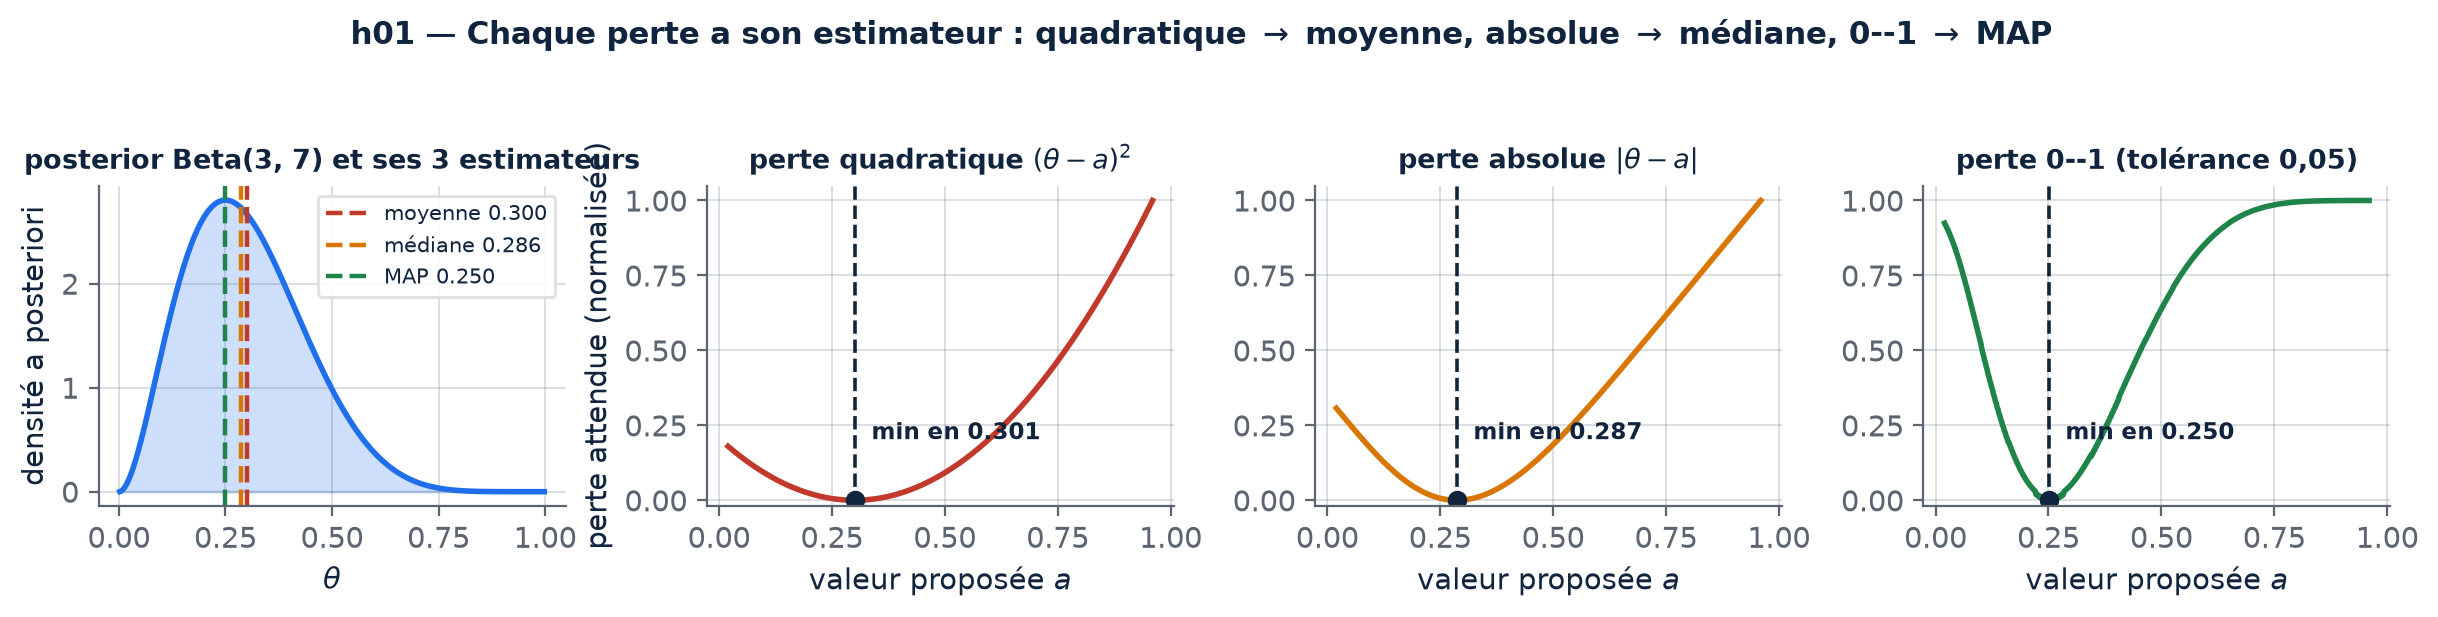
\includegraphics[width=.97\textwidth]{h01_estimateurs_pertes.png}
\end{center}
\vspace{-1mm}
\begin{columns}[t]
\begin{column}{0.55\textwidth}
\begin{ebox}[Lecture du graphique (calculs exécutés)]
Posterior \textbf{Beta$(3,7)$}, franchement asymétrique à droite. Les trois
pertes, évaluées sur une grille de $470$ valeurs de $a$, atteignent leur minimum
en trois points distincts : \textbf{la courbe de perte tranche, elle ne discute pas}.
\end{ebox}
\end{column}
\begin{column}{0.43\textwidth}
\begin{solbox}[Minima numériques trouvés]
\resizebox{\ifdim\width>\linewidth\linewidth\else\width\fi}{!}{%
\begin{tabular}{@{}lll@{}}
\toprule
Perte & $a^\star$ trouvé & estimateur \\
\midrule
quadratique & $0{,}301$ & moyenne $0{,}300$ \\
absolue & $0{,}287$ & médiane $0{,}286$ \\
0--1 ($\varepsilon{=}0{,}05$) & $0{,}250$ & mode $0{,}250$ \\
\bottomrule
\end{tabular}}
\vspace{1mm}

\tiny Écart mode -- moyenne : $0{,}050$ sur une échelle $[0\,;1]$, soit
$5$ points de taux : en industrie, ce n'est pas un détail.
\end{solbox}
\end{column}
\end{columns}
\end{frame}

% ---------------------------------------------------------------- 8
\begin{frame}{Tableau de bord : le posterior Beta$(3,7)$ en chiffres}
\small
\vspace{-1mm}
\begin{columns}[t]
\begin{column}{0.48\textwidth}
\begin{ebox}[Ce que la machine a calculé]
\begin{itemize}
  \item moyenne $\E[\theta \given y] = 0{,}300$
  \item médiane $= 0{,}286$
  \item mode (MAP) $= 0{,}250$
  \item $\argmin$ perte quadratique $= 0{,}301$
  \item $\argmin$ perte absolue $= 0{,}287$
  \item $\argmin$ perte 0--1 $= 0{,}250$
\end{itemize}
\vspace{1mm}
\footnotesize Les minima \emph{numériques} reproduisent les formules théoriques à
$0{,}001$ près : c'est la vérification qui doit être faite \textbf{avant} de faire
confiance à un code d'optimisation.
\end{ebox}
\end{column}
\begin{column}{0.50\textwidth}
\begin{kbox}[Le réflexe d'ingénieur]
\begin{enumerate}
  \item Calculer la moyenne (toujours possible, gratuite).
  \item Regarder l'\textbf{asymétrie} : si
        $\E[\theta \given y] \neq $ médiane, la moyenne est un choix, pas un dû.
  \item Demander au commanditaire : « que coûte une erreur de $+0{,}05$ ? et de $-0{,}05$ ? »
  \item Choisir l'estimateur, et \textbf{l'annoncer dans le rapport}.
\end{enumerate}
\end{kbox}
\end{column}
\end{columns}
\vspace{1mm}
\begin{wbox}[Ne jamais faire]
Rapporter la sortie par défaut de la librairie sans dire \textbf{de quelle perte}
elle correspond : \py{np.mean()} minimise l'erreur quadratique. Si le client paie
une perte absolue, vous n'avez pas optimisé \emph{son} problème.
\end{wbox}
\end{frame}

% ---------------------------------------------------------------- 9
\begin{frame}{Quiz --- Quelle perte pour quelle décision ?}
\begin{qbox}[Question 1 --- Rupture de stock]
Un magasin choisit la quantité $a$ à commander. Une rupture coûte cinq fois plus
qu'un invendu. La perte est
$L(\theta,a)=c|\theta-a|$ avec $c = 5$ si $a<\theta$, $c=1$ si $a>\theta$.
Quel résumé du posterior faut-il viser ?
\vspace{1.5mm}
\begin{enumerate}
  \item[(A)] la moyenne
  \item[(B)] la médiane
  \item[(C)] un \textbf{quantile supérieur} : $P(\theta \leq a \given y) \approx \frac{c_+}{c_+ + c_-}$
  \item[(D)] le mode
\end{enumerate}
\vspace{1mm}
\textbf{Réponse : (C).} La médiane correspondrait à $c_+ = c_-$. Le calcul de
$\rho'(a) = c_+ P(\theta > a \given y) - c_- P(\theta < a \given y)$ donne
$P(\theta > a \given y) = \frac{c_-}{c_+ + c_-} = \frac{1}{6}$, soit le
\textbf{quantile d'ordre $5/6 \approx 83{,}3\,\%$}.
\end{qbox}
\vspace{1mm}
\begin{kbox}[Le message]
\small Aucun estimateur n'est « bayésien » tout seul : \textbf{l'estimateur est
défini par la perte}. Changer la perte, c'est changer la réponse --- et c'est
exactement ce qu'on veut.
\end{kbox}
\end{frame}

% ---------------------------------------------------------------- 10
\begin{frame}{MAP contre maximum de vraisemblance}
\small
\vspace{-1mm}
\begin{columns}[t]
\begin{column}{0.52\textwidth}
\begin{kbox}[Deux arguments, à un terme près]
\[
\text{MAP} = \argmax_\theta \; \underbrace{p(\theta \given y)}_{\propto\, p(y \given \theta) p(\theta)}
\qquad\qquad
\text{MLE} = \argmax_\theta \; p(y \given \theta)
\]
En passant au logarithme :
\[
\log p(\theta \given y) = \log p(y \given \theta) + \log p(\theta) + \text{cste}.
\]
Le prior n'est donc rien d'autre qu'une \textbf{pénalité} ajoutée à la
log-vraisemblance --- ce que les statisticiens appellent une régularisation.
\end{kbox}
\end{column}
\begin{column}{0.46\textwidth}
\begin{ebox}[Lecture moderne]
\begin{itemize}
  \item Prior uniforme $\Rightarrow$ MAP $=$ MLE.
  \item Prior $\N(0, \tau^2)$ $\Rightarrow$ pénalité $\ell_2$
        (crête / \textit{ridge}).
  \item Prior Laplace $\Rightarrow$ pénalité $\ell_1$
        (lasso, parcimonie).
  \item Prior Beta$(\alpha_0, \beta_0)$ $\Rightarrow$ moyenne a posteriori
        $=$ compteur de succès et d'échecs \textbf{ajoutés} aux données.
\end{itemize}
\end{ebox}
\end{column}
\end{columns}
\vspace{1mm}
\begin{wbox}[La différence de fond avec le MLE]
Le MLE est \textbf{invariant} par reparamétrisation ($\hat\theta$ et $g(\hat\theta)$ se correspondent). Le MAP
n'est \textbf{pas} invariant : changer de paramètre change le prior, donc change
le mode. \textbf{La moyenne a posteriori}, elle, se transforme correctement.
\end{wbox}
\end{frame}

% ---------------------------------------------------------------- 11
\begin{frame}{Exemple chiffré : Beta-Bernoulli, $k = 14$ succès sur $n = 20$}
\begin{columns}[t]
\begin{column}{0.47\textwidth}
\begin{ebox}[Les deux estimateurs, en formules]
\small
Avec $n_0 = \alpha_0 + \beta_0$ et $m_0 = \alpha_0/n_0$ :
\[
\hat\theta_{\text{MLE}} = \frac{k}{n} = \frac{14}{20} = 0{,}700
\]
\[
\theta_{\text{MAP}} = \frac{k + \alpha_0 - 1}{n + \alpha_0 + \beta_0 - 2}
\]
\[
\E[\theta \given y] = \frac{k + \alpha_0}{n + \alpha_0 + \beta_0}
= \frac{k + n_0 m_0}{n + n_0}
\]
\end{ebox}
\end{column}
\begin{column}{0.51\textwidth}
\begin{solbox}[Prior centré sur $0{,}40$]
\resizebox{\ifdim\width>\linewidth\linewidth\else\width\fi}{!}{%
\begin{tabular}{@{}lccc@{}}
\toprule
Force du prior & moyenne a post. & MAP & poids des données \\
\midrule
$n_0 = 2$   & $0{,}673$ & $0{,}690$ & $0{,}909$ \\
$n_0 = 10$  & $0{,}600$ & $0{,}607$ & $0{,}667$ \\
$n_0 = 100$ & $0{,}450$ & $0{,}449$ & $0{,}167$ \\
\midrule
\multicolumn{4}{@{}l@{}}{\textbf{MLE (le prior est ignoré)} : $0{,}700$} \\
\bottomrule
\end{tabular}}
\vspace{1.5mm}

\small Le poids des données est $\frac{n}{n+n_0}$ : c'est la \textbf{formule de la
moyenne pondérée} entre ce que disent les données et ce que dit le prior.
\end{solbox}
\end{column}
\end{columns}
\vspace{1mm}
\begin{abox}[Exercice éclair (3 min, en binôme)]
Avec $n = 20$, $k = 14$ et un prior centré sur $0{,}40$ : quel $n_0$ rend données
et prior équipondérés, et quelle est alors la moyenne a posteriori ?
\vspace{0.5mm}

\textbf{Réponse :} $n_0 = n = 20$ ($w = 0{,}5$) et
$0{,}5 \times 0{,}70 + 0{,}5 \times 0{,}40 = 0{,}55$.
\end{abox}
\end{frame}

% ---------------------------------------------------------------- 12
\begin{frame}{Visualiser le \textit{shrinkage} : le MAP est tiré vers le prior}
\small
\vspace{-1.5mm}
\begin{center}
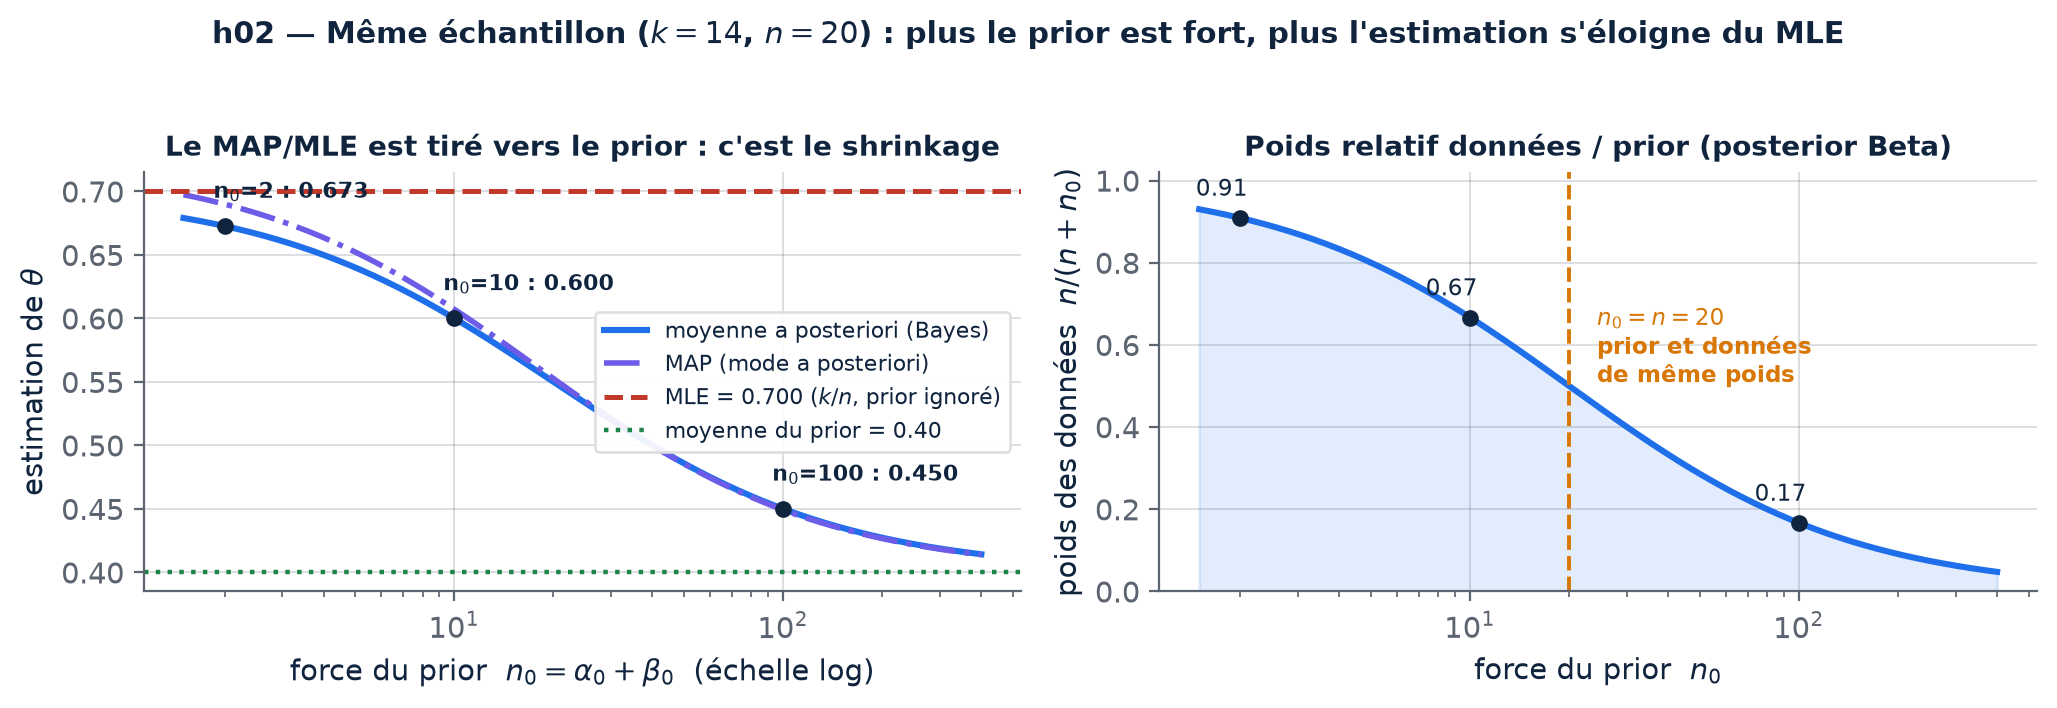
\includegraphics[width=.84\textwidth]{h02_shrinkage_prior.png}
\end{center}
\vspace{-1.5mm}
\begin{columns}[t]
\begin{column}{0.62\textwidth}
\begin{ebox}[Ce que montrent les deux panneaux]
Le MLE vaut $0{,}700$ et ne bouge jamais. La moyenne a posteriori et le MAP
s'en écartent d'autant plus que le prior est fort, et \textbf{convergent} vers
$0{,}700$ quand $n_0 \to 0$. Pour $n_0 = n = 20$, prior et données pèsent
exactement pareil : la moyenne tombe à mi-chemin entre $0{,}40$ et $0{,}70$.
\end{ebox}
\end{column}
\begin{column}{0.36\textwidth}
\begin{kbox}[Shrinkage]
Le terme anglais signifie « rétraction » : l'estimation est
\textbf{rétractée} vers le centre du prior. Ce n'est pas un défaut de méthode,
c'est exactement ce qui \textbf{réduit le risque} aux petits échantillons
(section 3.4, figure du MSE).
\end{kbox}
\end{column}
\end{columns}
\end{frame}

% ---------------------------------------------------------------- 13
\begin{frame}{Biais, variance et shrinkage : le vrai mécanisme}
\begin{columns}[t]
\begin{column}{0.49\textwidth}
\begin{ebox}[Décomposition biais--variance (fréquentiste)]
Pour $\hat\theta$ estimant $\theta$ :
\[
\E[(\hat\theta - \theta)^2]
= \underbrace{\big(\E[\hat\theta] - \theta\big)^2}_{\text{biais}^2}
+ \underbrace{\Var(\hat\theta)}_{\text{variance}} .
\]
Le MLE est \textbf{sans biais} mais de variance $\frac{\theta(1-\theta)}{n}$.
La moyenne a posteriori est \textbf{biaisée} (vers la croyance a priori) mais de
variance plus faible : le compromis peut améliorer le MSE total.
\end{ebox}
\end{column}
\begin{column}{0.49\textwidth}
\begin{solbox}[MSE mesuré : 500 simulations]
\resizebox{\ifdim\width>\linewidth\linewidth\else\width\fi}{!}{%
\begin{tabular}{@{}lccc@{}}
\toprule
$n$ & MSE (MLE) & MSE (Bayes) & rapport \\
\midrule
$5$   & $0{,}04526$ & $0{,}01853$ & $\mathbf{0{,}41}$ \\
$20$  & --- & --- & $0{,}74$ \\
$400$ & $0{,}000518$ & $0{,}000518$ & $1{,}00$ \\
\bottomrule
\end{tabular}}
\vspace{1.5mm}
\tiny Aux petits échantillons, le bayésien divise le risque par $\approx 2{,}4$ ;
à $n = 400$, l'avantage disparaît : \textbf{les données prennent le pouvoir}.
\end{solbox}
\end{column}
\end{columns}
\vspace{1mm}
\begin{kbox}[La formule du compromis, en une ligne]
La moyenne a posteriori est un \textbf{estimateur rétréci} :
$a^\star = w\,\hat\theta_{\text{MLE}} + (1-w)\, m_0$ avec $w = \frac{n}{n+n_0}$.
Optimiser $w$ revient à optimiser le compromis biais--variance.
\end{kbox}
\end{frame}

% ---------------------------------------------------------------- 14
\begin{frame}{Activité guidée --- 8 minutes, par binômes}
\begin{abox}[Énoncé]
Un posterior est $\mathrm{Beta}(3, 7)$. On dispose de Python et de
\file{scipy.stats}.
\begin{enumerate}
  \item Calculez \textbf{à la main} la moyenne, la médiane et le mode.
  \item Retrouvez-les avec \py{stats.beta(3,7).mean()} et
        \py{stats.beta(3,7).median()}.
  \item Écrivez une boucle qui évalue $\rho(a)$ pour les trois pertes sur
        \py{a} de $0{,}02$ à $0{,}96$, et vérifiez les minima trouvés.
  \item \textbf{Question subsidiaire} : pour quelle valeur de $c_+/c_-$ la
        perte absolue asymétrique du slide 4 donne-t-elle exactement la moyenne ?
\end{enumerate}
\end{abox}
\vspace{1mm}
\begin{columns}[t]
\begin{column}{0.49\textwidth}
\begin{solbox}[Résultats attendus (vérifiés par le script du cours)]
moyenne $0{,}300$, médiane $0{,}286$, mode $0{,}250$ ;
minima numériques $0{,}301$, $0{,}287$, $0{,}250$.
\end{solbox}
\end{column}
\begin{column}{0.49\textwidth}
\begin{kbox}[Subsidiaire, la réponse]
Non : avec $c_+ = c_-$ on retombe sur la médiane. Pour obtenir la moyenne, il
faut une perte quadratique : une pénalité qui croît avec le \emph{carré} de
l'écart, et non linéairement.
\end{kbox}
\end{column}
\end{columns}
\end{frame}

% ---------------------------------------------------------------- 15
\begin{frame}{Synthèse de la section 3.1}
\begin{center}
{\small
\begin{tabular}{@{}p{0.16\textwidth}p{0.14\textwidth}p{0.12\textwidth}p{0.40\textwidth}@{}}
\toprule
\textbf{Perte} & \textbf{Estimateur} & \textbf{symboles} & \textbf{Propriétés / précautions} \\
\midrule
quadratique $(\theta-a)^2$ & moyenne & $\E[\theta \given y]$ &
toujours définie, se transforme bien ; sensible aux queues épaisses \\
\addlinespace
absolue $|\theta-a|$ & médiane & $q_{0{,}5}$ &
robuste ; cohérente avec le HDI ; pas de formule fermée simple \\
\addlinespace
0--1 & mode (MAP) & $\argmax p(\theta \given y)$ &
lien direct avec le MLE et la régularisation ; \textbf{non invariant} par
reparamétrisation \\
\addlinespace
asymétrique & quantile & $q_{\,c_+/(c_++c_-)}$ &
traduit les coûts réels du métier (rupture, crue, fraude) \\
\bottomrule
\end{tabular}}
\end{center}
\vspace{1.5mm}
\begin{kbox}[À retenir en une phrase]
Un estimateur ponctuel n'est pas « la réponse » : c'est \textbf{la réponse à une
question de coût}. Le posterior est le même pour tous ; seule la perte change.
\end{kbox}
\end{frame}

% ---------------------------------------------------------------- 16
\begin{frame}{Section 3.2 --- Du point à l'intervalle : trois constructions}
\small
\vspace{-1mm}
\begin{columns}[t]
\begin{column}{0.31\textwidth}
\begin{ebox}[1. Queues égales]
On coupe $2{,}5\,\%$ de masse de chaque côté :
$[q_{0{,}025}\,;\,q_{0{,}975}]$.

\vspace{1mm}\footnotesize Valeur par défaut : une ligne de code, se résume bien.
\end{ebox}
\end{column}
\begin{column}{0.31\textwidth}
\begin{ebox}[2. HDI (densité postérieure la plus élevée)]
L'intervalle \textbf{le plus court} de masse $0{,}95$ : chaque point dedans a une
densité supérieure à chaque point dehors.

\vspace{1mm}\footnotesize Indispensable pour les posteriors fortement asymétriques
(Gamma, Beta extrêmes).
\end{ebox}
\end{column}
\begin{column}{0.33\textwidth}
\begin{ebox}[3. Unilatéral]
\scriptsize
Le seuil $\theta_0$ est-il dépassé ? On annonce
$q_{5\%}$ et $P(\theta > \theta_0 \given y)$.

\vspace{1mm} Répond à une question de décision.
\end{ebox}
\end{column}
\end{columns}
\vspace{-0.5mm}
\begin{kbox}[Définition d'un intervalle de crédibilité de niveau $1-\alpha$]
Tout ensemble $C \subset \Theta$ tel que
\[
P(\theta \in C \given y) = \int_C p(\theta \given y)\,\mathrm{d}\theta = 1-\alpha .
\]
Il n'y a donc \emph{pas unicité} : le choix des bornes est une décision
supplémentaire.
\end{kbox}
\end{frame}

% ---------------------------------------------------------------- 17
\begin{frame}{HDI contre queues égales : le plus court gagne}
\small
\vspace{-2mm}
\begin{center}
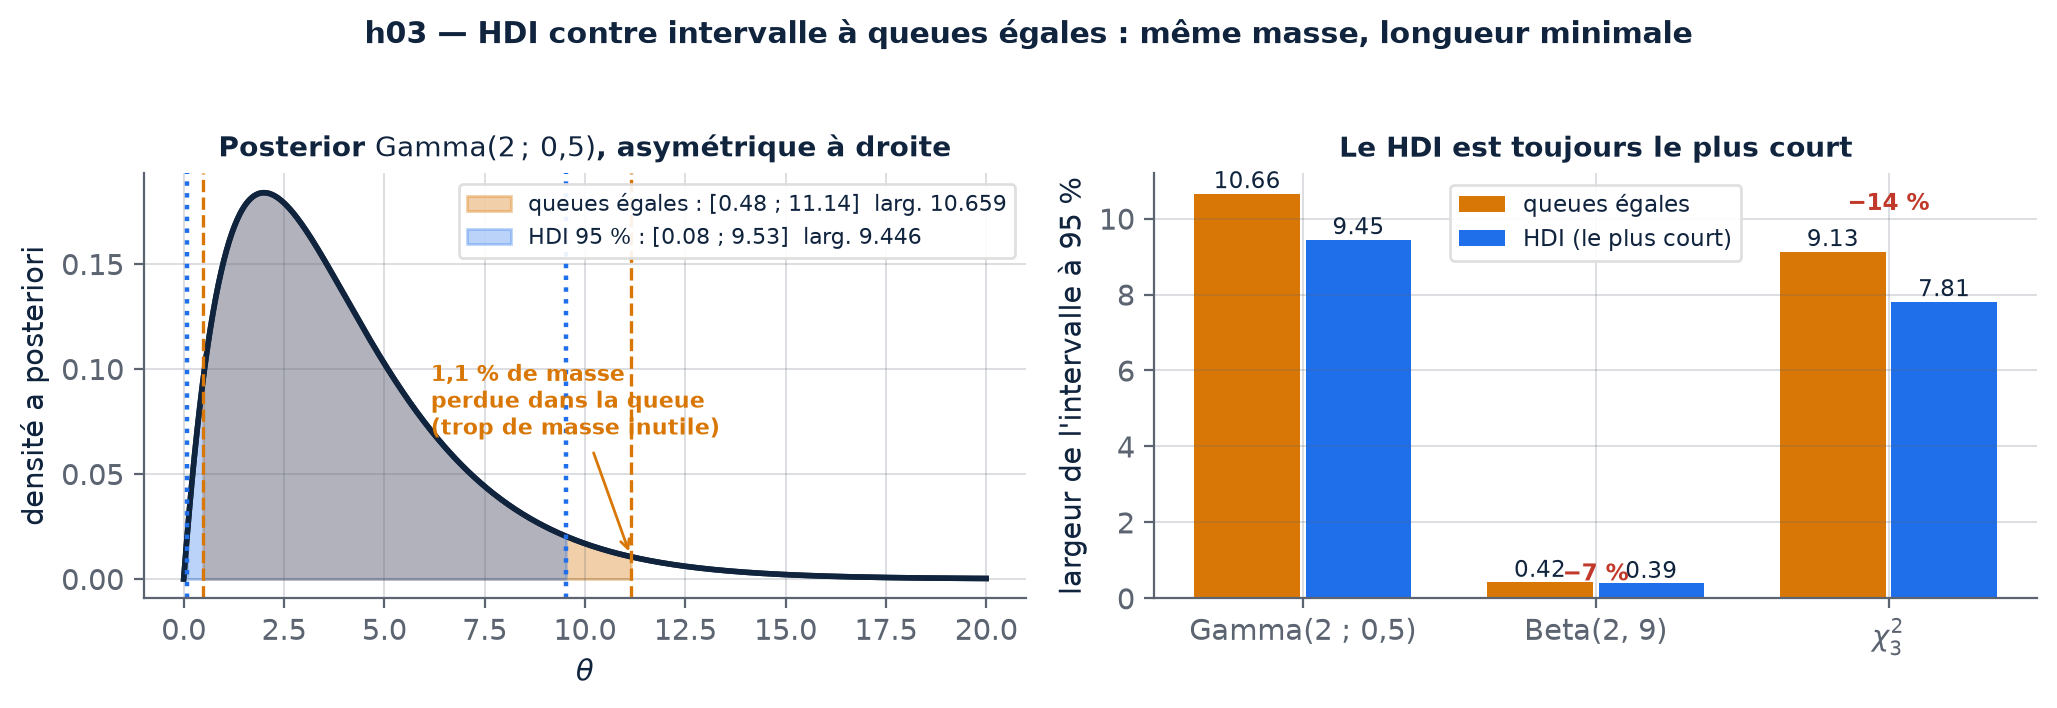
\includegraphics[width=.80\textwidth]{h03_hdi_vs_queue.png}
\end{center}
\vspace{-2.5mm}
\begin{columns}[t]
\begin{column}{0.56\textwidth}
\begin{ebox}[Calculs exécutés sur trois posteriors asymétriques]
\small
\begin{tabular}{@{}lccc@{}}
\toprule
Posterior & queues égales & HDI 95 \% & gain \\
\midrule
Gamma$(2\,;\,0{,}5)$ & $[0{,}484\,;\,11{,}143]$ & $[0{,}080\,;\,9{,}526]$ & $-11{,}4\,\%$ \\
Beta$(2,9)$ & largeur $0{,}4198$ & largeur $0{,}3905$ & $-7{,}0\,\%$ \\
$\chi^2_3$ & largeur $9{,}133$ & largeur $7{,}814$ & $-14{,}4\,\%$ \\
\bottomrule
\end{tabular}
\end{ebox}
\end{column}
\begin{column}{0.42\textwidth}
\begin{kbox}[Pourquoi l'écart existe]
L'intervalle à queues égales coupe \textbf{en probabilité} ($2{,}5\,\%$ de chaque
côté), pas \textbf{en densité}. Sur une loi à queue droite épaisse, il garde des
valeurs très improbables à droite pour satisfaire la symétrie de masse.
Le HDI, lui, coupe là où la densité est égale : sa largeur est minimale.
\end{kbox}
\end{column}
\end{columns}
\end{frame}
\nb{50}

% =====================================================================
%  CHAPITRE 3 -- partie b : sections 3.2 (fin) et 3.3
% =====================================================================

% ---------------------------------------------------------------- 18
\begin{frame}{HDI : la définition rigoureuse}
\small
\vspace{-1mm}
\begin{kbox}[Densité postérieure la plus élevée (\textit{Highest Density Interval})]
Pour un posterior $p(\theta \given y)$ et un niveau $1-\alpha$, le HDI est
l'ensemble
\[
C_{\text{HDI}} = \big\{\theta : p(\theta \given y) \geq h_{1-\alpha}\big\}
\quad\text{où}\quad h_{1-\alpha} \text{ est le seuil tel que } P(C_{\text{HDI}} \given y) = 1-\alpha .
\]
Conséquence immédiate : \textbf{toute valeur à l'intérieur a une densité
postérieure supérieure à toute valeur à l'extérieur}. C'est donc, parmi tous les
ensembles de masse $1-\alpha$, celui de \textbf{plus petite longueur}.
\end{kbox}
\vspace{1mm}
\begin{columns}[t]
\begin{column}{0.49\textwidth}
\begin{ebox}[Posterior unimodal --- le cas courant]
Le HDI est un intervalle $[a, b]$, solution de
\[
p(a \given y) = p(b \given y) \quad\text{et}\quad \int_a^b p(\theta \given y)\mathrm{d}\theta = 1-\alpha .
\]
Les bornes ont donc \textbf{la même densité} : c'est le test d'arrêt à utiliser
dans un code.
\end{ebox}
\end{column}
\begin{column}{0.49\textwidth}
\begin{wbox}[Posterior multimodal ou à plateau]
Le HDI n'est plus un intervalle : c'est une \textbf{union} de morceaux
(ex. un bimodal donne deux intervalles séparés). Ne jamais dire « le » HDI
sans vérifier l'unimodalité. Un intervalle à queues égales, lui, reste toujours
un intervalle --- mais peut être très large.
\end{wbox}
\end{column}
\end{columns}
\end{frame}

% ---------------------------------------------------------------- 19
\begin{frame}[fragile]{Calculer un HDI : code exact (et version ArviZ)}
\footnotesize
\vspace{-2mm}
\begin{codebox}[Recherche du plus court intervalle de masse $0{,}95$ sur une grille]
\begin{lstlisting}
import numpy as np
from scipy import stats

def hdi_grid(dist, level=0.95, m=200_001):
    x = np.linspace(0.0, float(dist.ppf(1 - 1e-7)), m)
    dens = dist.pdf(x)
    c = np.concatenate([[0.0], np.cumsum((dens[1:] + dens[:-1]) / 2 * np.diff(x))])
    c /= c[-1]                    # fonction de repartition cumulee (trapezes)
    j = np.searchsorted(c, c + level)      # borne droite pour chaque borne gauche
    w = np.where(j < m, x[np.clip(j, 0, m - 1)] - x, np.inf)
    i = int(np.argmin(w))                  # on garde le plus court
    return float(x[i]), float(x[np.clip(j[i], 0, m - 1)])

print(hdi_grid(stats.gamma(a=2.0, scale=2.0)))            # (0.080 ; 9.526)
print(stats.gamma(a=2.0, scale=2.0).ppf([.025, .975]))    # (0.484 ; 11.143)
\end{lstlisting}
\end{codebox}
\vspace{0.5mm}
\begin{columns}[t]
\begin{column}{0.55\textwidth}
\begin{ebox}[Avec ArviZ, sur des tirages MCMC]
\py{az.hdi(draws, hdi_prob=0.95)} renvoie directement les bornes ; c'est
l'équivalent de notre fonction, appliqué à un échantillon au lieu d'une densité
analytique.
\end{ebox}
\end{column}
\begin{column}{0.43\textwidth}
\begin{kbox}[Vérification faite en cours]
Notre fonction donnait $[0{,}484\,;11{,}143]$ à queues égales contre
$[0{,}080\,;9{,}526]$ en HDI pour Gamma$(2\,;0{,}5)$ : $11{,}4\,\%$ de largeur
en moins, calculé, pas supposé.
\end{kbox}
\end{column}
\end{columns}
\end{frame}

% ---------------------------------------------------------------- 20
\begin{frame}{Crédibilité unilatérale : la question du décideur}
\begin{center}
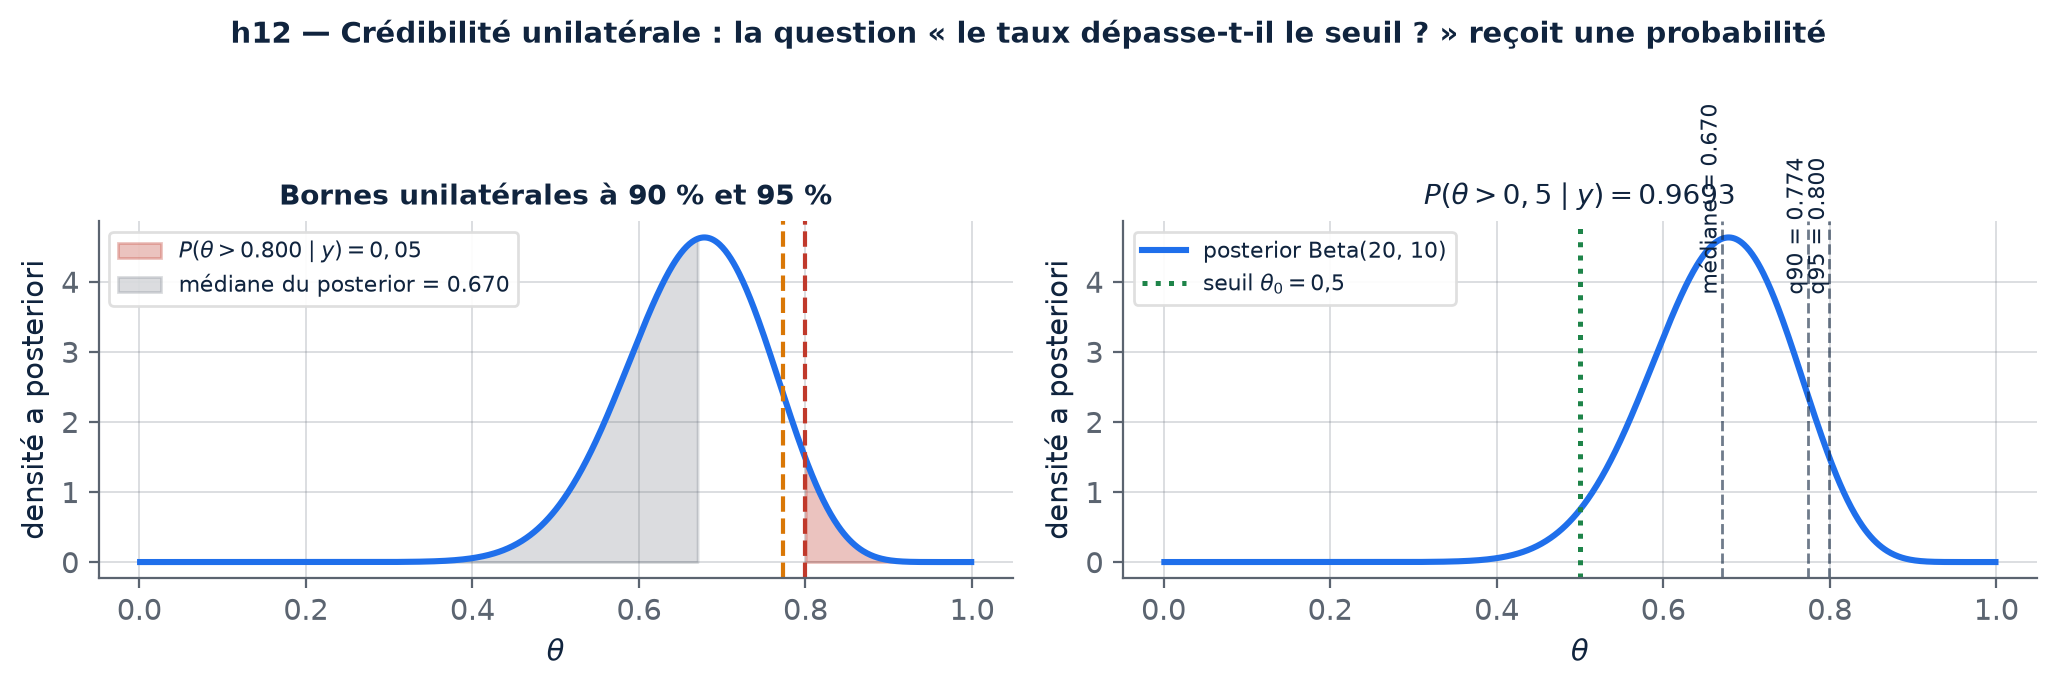
\includegraphics[width=.88\textwidth]{h12_credibilite_unilaterale.png}
\end{center}
\end{frame}

\begin{frame}{Crédibilité unilatérale : la question du décideur}
\small
\begin{columns}[t]
\begin{column}{0.48\textwidth}
\begin{ebox}[Posterior Beta$(20,10)$]
\resizebox{\ifdim\width>\linewidth\linewidth\else\width\fi}{!}{%
\begin{tabular}{@{}lc@{}}
\toprule
Quantile du posterior & valeur \\
\midrule
médiane $q_{0{,}50}$ & $0{,}670$ \\
$q_{0{,}90}$ & $0{,}774$ \\
$q_{0{,}95}$ & $0{,}800$ \\
\bottomrule
\end{tabular}}
\vspace{1.5mm}

$P(\theta > 0{,}5 \given y) = \mathbf{0{,}9693}$
\end{ebox}
\end{column}
\begin{column}{0.48\textwidth}
\begin{solbox}[Trois phrases possibles]
\footnotesize
\begin{itemize}
  \item « au moins $50\,\%$ de chance que $\theta > 0{,}670$ » ;
  \item « le taux dépasse $0{,}5$ à $96{,}9\,\%$ de probabilité » ;
  \item « borne supérieure à $90\,\%$ : $0{,}774$ ».
\end{itemize}
\end{solbox}
\end{column}
\end{columns}
\vspace{1mm}
\begin{kbox}[Unilatéral contre bilatéral]
$[q_{0{,}05} ; +\infty[$ et $]-\infty ; q_{0{,}95}]$ ont chacun $95\,\%$ de masse,
mais ils ne répondent pas à la même question. Le décideur veut presque toujours
un \textbf{unilatéral} (« est-ce au-dessus du seuil ? »), le statisticien publie
souvent un bilatéral par habitude.
\end{kbox}
\end{frame}

% ---------------------------------------------------------------- 21
\begin{frame}{Quiz --- Intervalles : le bon outil au bon moment}
\begin{qbox}[Quatre situations, quatre intervalles]
Pour chaque cas, choisissez l'outil correct et justifiez en une ligne.
\vspace{1mm}
\begin{enumerate}
  \item[(1)] Posterior Beta$(0{,}5, 0{,}5)$ très asymétrique : on veut « l'intervalle
        à $95\,\%$ » pour un graphique de synthèse.
  \item[(2)] Le régulateur demande : « le taux de défaut est-il \emph{sous} $2\,\%$ ? »
  \item[(3)] On publie un tableau comparatif avec des IC fréquentistes :
        on veut la comparaison la moins biaisée possible.
  \item[(4)] Posterior bimodal (mélange de deux populations) : on veut
        « l'intervalle à $95\,\%$ ».
\end{enumerate}
\vspace{1mm}
\textbf{Réponses :} (1) HDI, nettement plus court ; (2) \textbf{unilatéral}
$]-\infty\,;q_{0{,}95}]$ avec la probabilité annoncée ; (3) queues égales
(identique à l'IC quand le prior est plat) ; (4) \textbf{aucun intervalle unique} :
il faut publier l'union des deux morceaux, ou traiter les deux sous-populations
séparément.
\end{qbox}
\end{frame}

% ---------------------------------------------------------------- 22
\begin{frame}{Tableau comparatif : IC fréquentiste contre intervalle crédible}
\small
\vspace{-2mm}
\begin{center}
{\footnotesize
\begin{tabular}{@{}p{0.14\textwidth}p{0.34\textwidth}p{0.40\textwidth}@{}}
\toprule
\textbf{Critère} & \textbf{Intervalle de confiance (fréquentiste)} & \textbf{Intervalle de crédibilité (bayésien)} \\
\midrule
Objet aléatoire & l'\textbf{intervalle} (les données changent) & le \textbf{paramètre} $\theta$ \\
\addlinespace
Énoncé correct & « $95\,\%$ des intervalles ainsi construits contiennent $\theta$ » &
$P(\theta \in [a,b] \given y) = 0{,}95$ \\
\addlinespace
Énoncé incorrect & « \nok{} il y a $95\,\%$ de chance que $\theta$ soit dedans » &
« \nok{} $95\,\%$ des répétitions contiendront $\theta$ » \\
\addlinespace
Dépend du prior & non & \warn{} oui, explicitement \\
\addlinespace
Peut être asymétrique & rarement (transformations) & oui, et c'est un choix \\
\addlinespace
Interprétation métier & « précision de la méthode » &
« croyance actuelle sur la valeur » \\
\addlinespace
Avec $n$ grand, prior plat & référence & \ok{} coïncide numériquement \\
\bottomrule
\end{tabular}}
\end{center}
\vspace{1mm}
\begin{wbox}[La phrase à ne jamais prononcer]
\nok{} « Il y a $95\,\%$ de chance que la vraie valeur soit dans \emph{cet}
intervalle de confiance. » Un IC fréquentiste, une fois calculé, contient $\theta$
ou ne le contient pas : la probabilité est $0$ ou $1$. Seul l'intervalle
\emph{crédible} porte une probabilité sur $\theta$.
\end{wbox}
\end{frame}

% ---------------------------------------------------------------- 23
\begin{frame}{La garantie se mesure : couverture empirique sur 2\,000 échantillons}
\begin{center}
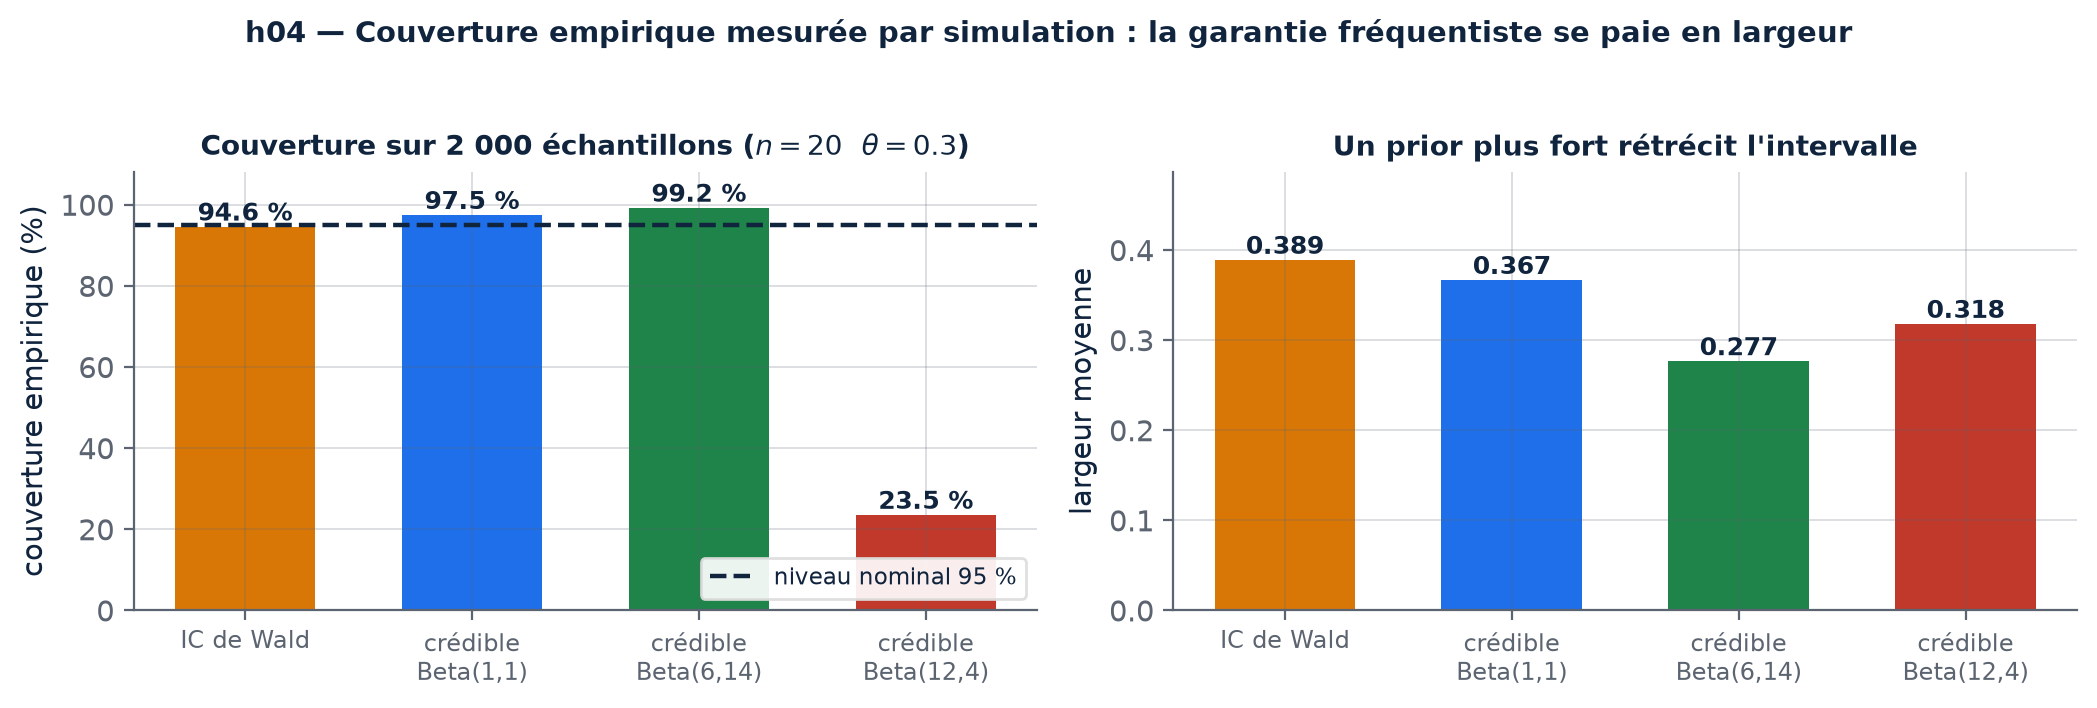
\includegraphics[width=.95\textwidth]{h04_couverture.png}
\end{center}
\vspace{-1.5mm}
\begin{columns}[t]
\begin{column}{0.60\textwidth}
\begin{ebox}[Protocole réellement exécuté]
$\theta_{\text{vrai}} = 0{,}30$, $n = 20$, \textbf{2\,000 échantillons} simulés
($k \sim \mathrm{Bin}(20 ; 0{,}30)$). Pour chacun, on calcule quatre intervalles à
$95\,\%$ et on teste s'ils contiennent $\theta_{\text{vrai}}$. On obtient la
fréquence de couverture --- la seule preuve honnête qu'un intervalle tient sa
promesse.
\end{ebox}
\end{column}
\begin{column}{0.38\textwidth}
\begin{solbox}[Couverture mesurée]
\small
\resizebox{\ifdim\width>\linewidth\linewidth\else\width\fi}{!}{%
\begin{tabular}{@{}lc@{}}
\toprule
Méthode & couverture \\
\midrule
IC de Wald & $94{,}6\,\%$ \\
crédible, prior Beta$(1,1)$ & $97{,}5\,\%$ \\
crédible, prior Beta$(6,14)$ & $99{,}3\,\%$ \\
crédible, prior Beta$(12,4)$ & \textcolor{byRed}{$23{,}6\,\%$} \\
\bottomrule
\end{tabular}}
\end{solbox}
\end{column}
\end{columns}
\end{frame}

% ---------------------------------------------------------------- 24
\begin{frame}{Ce que la couverture révèle (et ce qu'elle cache)}
\begin{columns}[t]
\begin{column}{0.49\textwidth}
\begin{ebox}[Lire le second panneau]
\begin{tabular}{@{}lcc@{}}
\toprule
Méthode & couverture & largeur moyenne \\
\midrule
IC de Wald & $94{,}6\,\%$ & $0{,}3891$ \\
Beta$(1,1)$ & $97{,}5\,\%$ & $0{,}3667$ \\
Beta$(6,14)$ & $99{,}3\,\%$ & $0{,}2766$ \\
Beta$(12,4)$ & $23{,}6\,\%$ & $0{,}3180$ \\
\bottomrule
\end{tabular}
\vspace{1.5mm}

\small Le prior \textbf{correct} (Beta$(6,14)$, centré sur $0{,}30$) rétrécit
l'intervalle de $29\,\%$ \emph{et} augmente la couverture : c'est le gain
authentique de l'information externe.
\end{ebox}
\end{column}
\begin{column}{0.49\textwidth}
\begin{wbox}[Le revers de la médaille]
Le prior Beta$(12,4)$ est centré sur $0{,}75$ alors que $\theta = 0{,}30$ :
l'intervalle crédible ne couvre la vérité que dans $23{,}6\,\%$ des cas
\emph{malgré} son étiquette « $95\,\%$ ». Un prior faux ne se contente pas de
rétrécir : il \textbf{ment avec assurance}.
\end{wbox}
\begin{kbox}[La règle d'or]
La garantie bayésienne est \textbf{conditionnelle au prior}. Sur des données
abondantes, tout prior raisonnable converge ; sur de petites données, la
couverture mesurée est l'outil de diagnostic obligatoire --- et elle se calcule.
\end{kbox}
\end{column}
\end{columns}
\end{frame}

% ---------------------------------------------------------------- 25
\begin{frame}{Activité --- Mesurez la couverture vous-mêmes (10 min)}
\begin{abox}[Protocole à coder en binôme]
\begin{enumerate}
  \item Simulez 2\,000 jeux de données : $k = $ \py{rng.binomial(20, 0.3, 2000)}.
  \item Pour chaque jeu, calculez l'IC de Wald
        $\hat p \pm 1{,}96\sqrt{\hat p(1-\hat p)/n}$.
  \item Puis l'intervalle crédible Beta$(1+k,\,1+n-k)$ (queues égales).
  \item Estimez la couverture : \py{np.mean((lo <= 0.3) & (0.3 <= hi))}.
  \item Recommencez avec $n = 5$, puis $n = 100$. Que devient la divergence entre
        les deux méthodes ?
\end{enumerate}
\end{abox}
\vspace{1mm}
\begin{columns}[t]
\begin{column}{0.49\textwidth}
\begin{solbox}[Résultats de référence ($n = 20$)]
Wald $94{,}6\,\%$ ; crédible Beta$(1,1)$ $97{,}5\,\%$.
L'IC de Wald \emph{sous}-couvre légèrement : c'est l'approximation normale, qui
néglige l'asymétrie du posterior à petit $n$.
\end{solbox}
\end{column}
\begin{column}{0.49\textwidth}
\begin{kbox}[Ce qu'il faut voir]
Aux petits $n$, le crédible à prior plat couvre \textbf{mieux} que l'IC classique :
la loi a posteriori exacte remplace une approximation asymptotique. C'est un
argument de robustesse, indépendant de tout a priori subjectif.
\end{kbox}
\end{column}
\end{columns}
\end{frame}

% ---------------------------------------------------------------- 26
\begin{frame}{Synthèse de la section 3.2 --- cinq règles}
\small
\vspace{-1mm}
\begin{columns}[t]
\begin{column}{0.49\textwidth}
\begin{kbox}[Les cinq règles]
\begin{enumerate}
  \item Toujours dire \textbf{quel} intervalle (queues égales, HDI, unilatéral).
  \item Sur un posterior asymétrique, préférer le \textbf{HDI}
        (jusqu'à $14\,\%$ plus court à masse égale).
  \item Pour une décision à seuil, publier un \textbf{unilatéral} et la
        probabilité $P(\theta > \theta_0 \given y)$.
  \item Ne jamais attribuer une probabilité à un IC fréquentiste.
  \item \textbf{Mesurer} la couverture par simulation avant de s'engager.
\end{enumerate}
\end{kbox}
\end{column}
\begin{column}{0.49\textwidth}
\begin{ebox}[Les chiffres de la section]
\resizebox{\ifdim\width>\linewidth\linewidth\else\width\fi}{!}{%
\begin{tabular}{@{}ll@{}}
\toprule
HDI sur Gamma$(2\,;0{,}5)$ & gain $11{,}4\,\%$ \\
HDI sur $\chi^2_3$ & gain $14{,}4\,\%$ \\
Couverture IC de Wald & $94{,}6\,\%$ \\
Couverture crédible Beta$(1,1)$ & $97{,}5\,\%$ \\
Couverture avec prior faux & $23{,}6\,\%$ \\
$P(\theta > 0{,}5)$ sur Beta$(20,10)$ & $0{,}9693$ \\
\bottomrule
\end{tabular}}
\vspace{1.5mm}
\tiny Toutes ces valeurs sortent de \file{src/fig\_ch3.py}, exécuté pour ce cours.
\end{ebox}
\end{column}
\end{columns}
\vspace{1mm}
\begin{tcolorbox}[colback=byCyan!8,colframe=byCyan,arc=2mm,width=.96\textwidth]
\centering\small
\textbf{Bascule vers 3.3} : un intervalle décrit $\theta$ ; le décideur, lui, veut
souvent \emph{la prochaine observation}. Ce n'est pas la même loi --- et c'est plus large.
\end{tcolorbox}
\end{frame}

% ---------------------------------------------------------------- 27
\begin{frame}{Section 3.3 --- Prédire : la loi prédictive a posteriori}
\small
\vspace{-1.5mm}
\begin{kbox}[Définition --- prédictive a posteriori]
\[
p(\tilde y \given y) \;=\; \int p(\tilde y \given \theta)\, p(\theta \given y)\, \mathrm{d}\theta .
\]
On \textbf{moyenne la vraisemblance de la nouvelle observation sur tout le
posterior} : on propage donc deux incertitudes --- celle du modèle
($p(\tilde y \given \theta)$) et celle du paramètre ($p(\theta \given y)$).
\end{kbox}
\vspace{1mm}
\begin{columns}[t]
\begin{column}{0.49\textwidth}
\begin{ebox}[Trois propriétés à connaître]
\begin{itemize}
  \item La prédictive est \textbf{toujours plus large} que la vraisemblance
        évaluée au point estimé : ignorer l'incertitude sur $\theta$, c'est
        sous-estimer le risque.
  \item Pour les couples conjugués, elle a une forme close
        (Beta-Binomial, Gamma-Poisson, Normal-Normal).
  \item Sans forme close, on l'approxime par \textbf{Monte-Carlo} :
        tirer $\theta^{(s)} \sim p(\theta \given y)$, puis
        $\tilde y^{(s)} \sim p(\tilde y \given \theta^{(s)})$.
\end{itemize}
\end{ebox}
\end{column}
\begin{column}{0.49\textwidth}
\begin{wbox}[Erreur classique]
\small Brancher le \emph{point estimate} dans le modèle et présenter la sortie
comme une prédiction : c'est ignorer $\Var(\theta \given y)$. L'intervalle obtenu
est trop étroit, donc \textbf{dangereux} (stocks, capacités, garanties). Pour
prédire, il faut la prédictive, pas la vraisemblance au mode.
\end{wbox}
\end{column}
\end{columns}
\end{frame}

% ---------------------------------------------------------------- 28
\begin{frame}{Prédiction a posteriori : le cas des accidents}
\small
\vspace{-2.5mm}
\begin{center}
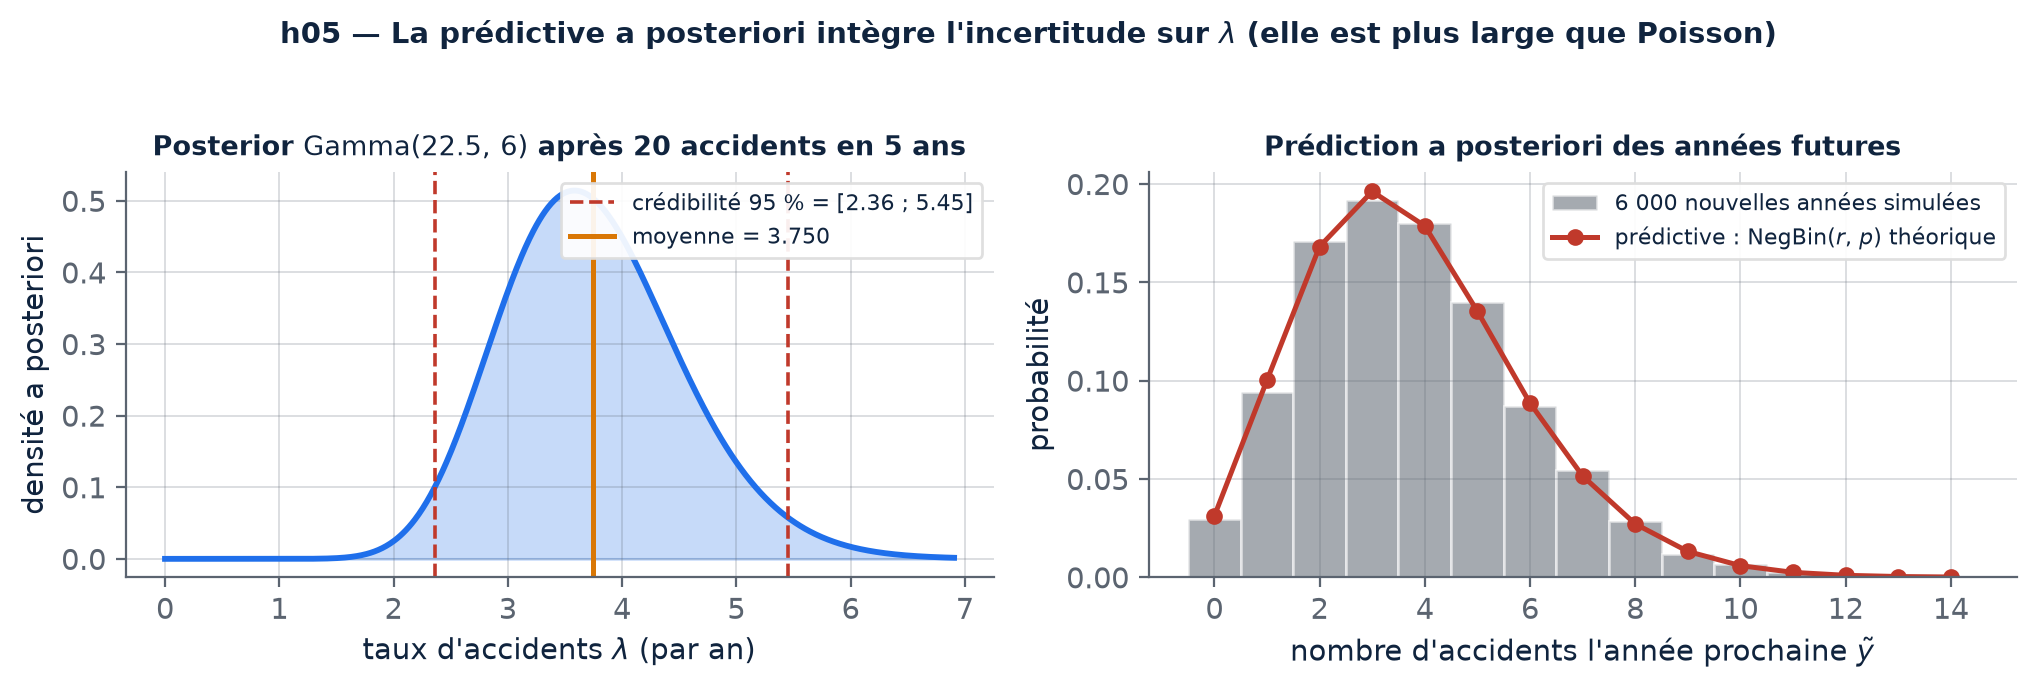
\includegraphics[width=.80\textwidth]{h05_predictive.png}
\end{center}
\vspace{-1.5mm}
\begin{columns}[t]
\begin{column}{0.55\textwidth}
\begin{ebox}[Données et posterior]
Un site a connu $4, 2, 5, 3, 6$ accidents sur cinq années, soit
\textbf{20 accidents} au total. Prior Gamma$(2{,}5\,;1)$ sur le taux annuel
$\lambda$ ; vraisemblance de Poisson.
\[
\lambda \given y \sim \mathrm{Gamma}(2{,}5 + 20 \,;\, 1 + 5)
= \mathrm{Gamma}(22{,}5\,;\,6)
\]
moyenne $3{,}75$ accidents par an, crédibilité $95\,\%$
$[2{,}36\,;5{,}45]$.
\end{ebox}
\end{column}
\begin{column}{0.43\textwidth}
\begin{solbox}[Lecture du gestionnaire]
\begin{itemize}
  \item $P(\lambda > 4 \given y) = 0{,}352$ : \warn{} un risque réel
        d'être au-dessus du seuil de $4$.
  \item $P(\tilde y > 6 \given y) = 0{,}102$ pour l'année prochaine.
  \item La probabilité d'une année \emph{sans} accident : $2{,}95\,\%$
        (simulation).
\end{itemize}
\end{solbox}
\end{column}
\end{columns}
\end{frame}

% ---------------------------------------------------------------- 29
\begin{frame}[fragile]{La prédictive sans formule : Monte-Carlo}
\begin{codebox}[Deux lignes de simulation, et la forme close pour vérifier]
\begin{lstlisting}
from scipy import stats
import numpy as np

obs = np.array([4, 2, 5, 3, 6])                 # 5 annees d'historique
a_post, b_post = 2.5 + obs.sum(), 1 + len(obs)  # posterior Gamma(22.5 ; 6)  [taux 6]
post = stats.gamma(a_post, scale=1 / b_post)

# --- predictive par Monte-Carlo (aucune formule necessaire) -----------------
lam_draws = post.rvs(20_000, random_state=4112)
y_new = np.random.default_rng(4112).poisson(lam_draws)

print(lam_draws.mean())                          # 3.75   moyenne a posteriori de lambda
print(np.percentile(lam_draws, [2.5, 97.5]))     # [2.36 ; 5.45]  credibilite 95 %
print(np.mean(y_new > 6))                        # 0.102  annee prochaine > 6 accidents
print(np.mean(y_new == 0))                       # 0.030  annee sans aucun accident

# --- verification par la forme close : Gamma-Poisson -> binomiale negative --
nb = stats.nbinom(a_post, b_post / (b_post + 1))
print(nb.sf(6))                                  # 0.1018 : accord a 1e-3 pres
\end{lstlisting}
\end{codebox}
\vspace{0mm}
\centering\footnotesize
Le Monte-Carlo et la formule exacte donnent la même réponse : c'est la
vérification croisée qui valide l'échantillonneur. Sorties réellement obtenues :
$3{,}75$, $[2{,}36\,;5{,}45]$, $0{,}102$, $0{,}030$, $0{,}1018$.
\end{frame}

% ---------------------------------------------------------------- 30
\begin{frame}{Posterior predictive check : le modèle sait-il reproduire les données ?}
\small
\vspace{-3mm}
\begin{center}
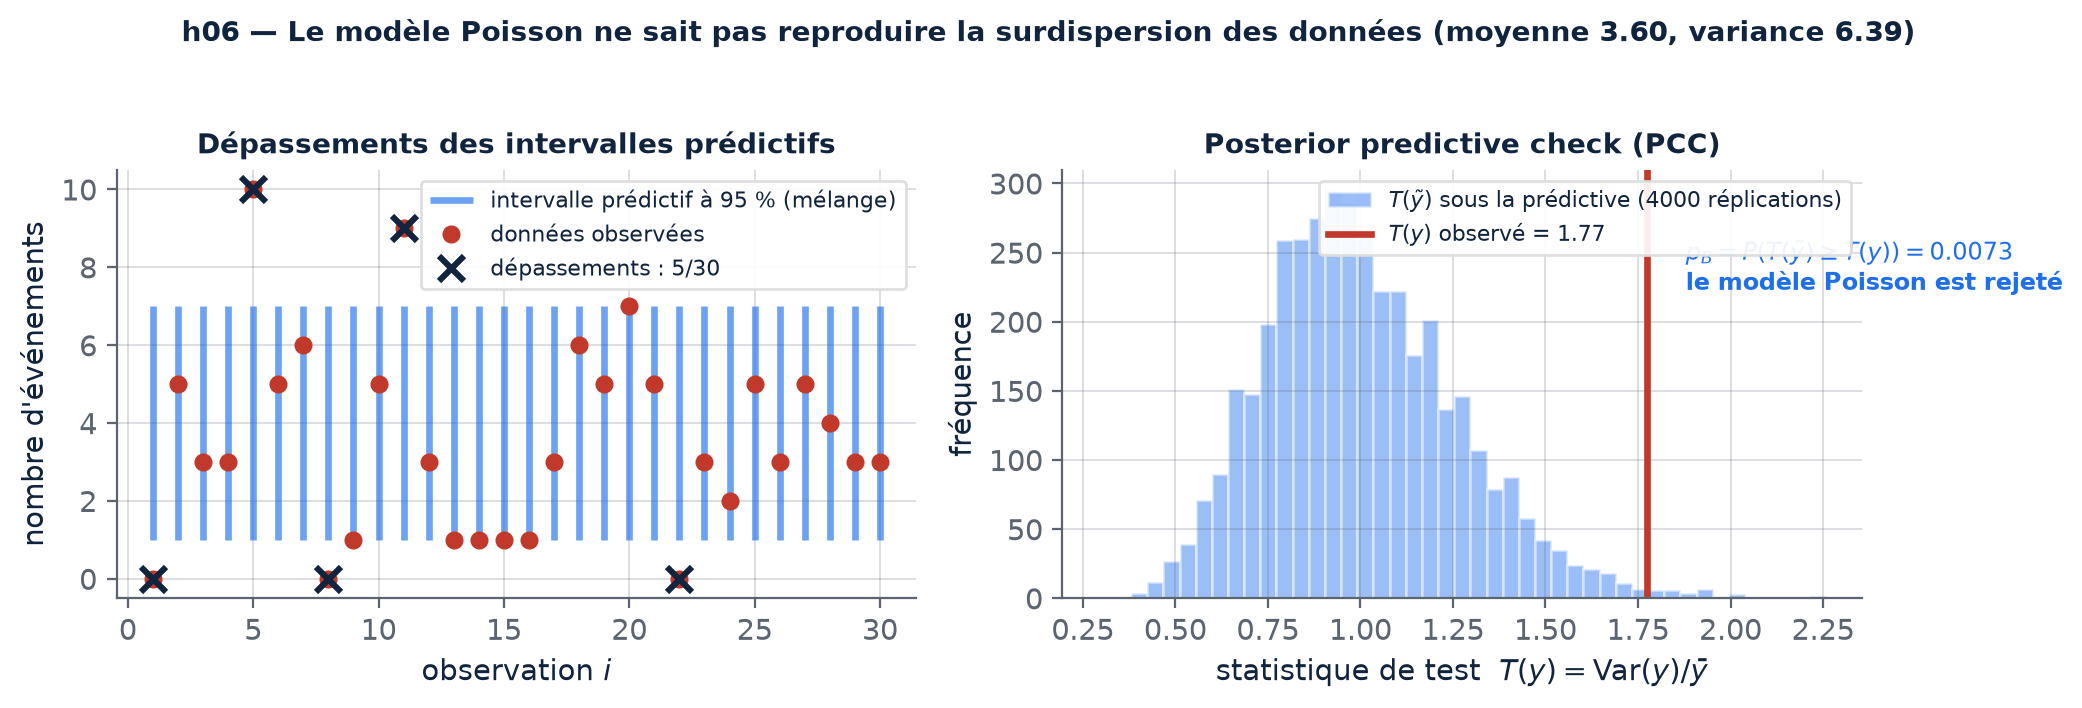
\includegraphics[width=.74\textwidth]{h06_ppc.png}
\end{center}
\vspace{-1.5mm}
\begin{columns}[t]
\begin{column}{0.55\textwidth}
\begin{ebox}[Protocole (Box, 1980)]
\begin{enumerate}
  \item Choisir une \textbf{statistique de test} $T(y)$ qui cible le défaut
        suspecté (ici la surdispersion : $T = \Var(y)/\bar y$).
  \item Tirer $\theta^{(s)} \sim p(\theta \given y)$ puis
        $\tilde y^{(s)} \sim p(\tilde y \given \theta^{(s)})$.
  \item Calculer la \textbf{probabilité a posteriori de queue}
        $p_B = P\big(T(\tilde y) \geq T(y) \given y\big)$.
\end{enumerate}
\end{ebox}
\end{column}
\begin{column}{0.43\textwidth}
\begin{solbox}[Résultat mesuré]
\begin{itemize}
  \item $T(y) = \Var(y)/\bar y = 1{,}774$ (moyenne $3{,}60$,
        variance $6{,}39$).
  \item $\mathbf{p_B = 0{,}0073}$ sur 4\,000 réplications.
  \item Depassements des intervalles prédictifs : $5/30$.
\end{itemize}
\vspace{1mm}
\footnotesize Conclusion : le modèle de Poisson \textbf{est rejeté}
(surdispersion).
\end{solbox}
\end{column}
\end{columns}
\end{frame}

% ---------------------------------------------------------------- 31
\begin{frame}{Lire un \textit{posterior predictive check} correctement}
\begin{columns}[t]
\begin{column}{0.49\textwidth}
\begin{kbox}[Ce que $p_B$ n'est pas]
\begin{itemize}
  \item \textbf{Pas} une $p$-value fréquentiste : c'est une probabilité a
        posteriori calculée \emph{sous le modèle}, sans hypothèse nulle.
  \item \textbf{Pas} une preuve de validité : un $p_B$ central ($\approx 0{,}5$)
        signifie seulement que la statistique choisie ne détecte rien.
  \item \textbf{Pas} un test de « vérité » du modèle : tous les modèles sont faux,
        certains sont utiles.
\end{itemize}
\end{kbox}
\end{column}
\begin{column}{0.49\textwidth}
\begin{ebox}[Ce $p_B$ dit vraiment]
Le modèle postule $\Var(y) = \E[y]$ (Poisson). Or la statistique observée
$1{,}774$ est plus grande que dans $99{,}3\,\%$ des réplications simulées.
Autrement dit : \textbf{même en tirant au hasard sous ce modèle, on n'obtient
presque jamais une variabilité aussi forte}. Il faut passer à une
binomiale négative (ou un modèle hiérarchique).
\end{ebox}
\end{column}
\end{columns}
\vspace{1mm}
\begin{wbox}[Le piège du dépassement isolé]
$5$ observations sur $30$ sortent de l'intervalle prédictif à $95\,\%$ : c'est
$16{,}7\,\%$ au lieu de $5\,\%$ attendus. Un dépassement ponctuel n'est pas
grave ; $5$ sur $30$ \textbf{avec} $p_B = 0{,}0073$, c'est un signal.
\end{wbox}
\end{frame}

% ---------------------------------------------------------------- 32
\begin{frame}{Activité --- Écrire un PPC de A à Z (12 min)}
\begin{abox}[Consigne]
On dispose du posterior du taux d'accidents $\mathrm{Gamma}(22{,}5\,;6)$ et du
modèle de Poisson.
\begin{enumerate}
  \item Choisissez \textbf{deux} statistiques de test : le maximum observé, et la
        proportion de valeurs nulles.
  \item Simulez $5\,000$ jeux de données de taille $n = 30$.
  \item Calculez $p_B$ pour chaque statistique.
  \item Conclusion : le modèle de Poisson est-il adapté aux données du site ?
\end{enumerate}
\end{abox}
\vspace{1mm}
\begin{columns}[t]
\begin{column}{0.49\textwidth}
\begin{solbox}[Résultats du cours, mêmes données]
$T = \Var(y)/\bar y$ : $T(y) = 1{,}774$ et $p_B = 0{,}0073$.
Les deux statistiques proposées ici explorent la même surdispersion sous un
autre angle.
\end{solbox}
\end{column}
\begin{column}{0.49\textwidth}
\begin{kbox}[Le réflexe professionnel]
Un PPC coûte dix lignes de code et évite des mois de conclusions fausses. Dans un
rapport, il se présente \textbf{avant} les résultats : « voici pourquoi ce modèle
est une description défendable de ces données ».
\end{kbox}
\end{column}
\end{columns}
\end{frame}

% ---------------------------------------------------------------- 33
\begin{frame}{Quiz --- Prédiction : les trois pièges}
\begin{qbox}[Question --- Le piège du point estimé]
Un ingénieur calcule $\E[\lambda \given y] = 3{,}75$ puis annonce : « l'année
prochaine, il y aura entre $3{,}75 \pm 1{,}96\sqrt{3{,}75}$, soit
$[0{,}05\,;7{,}45]$ accidents ». Qu'y a-t-il de faux ?
\vspace{1.5mm}
\begin{enumerate}
  \item[(A)] Rien : c'est l'intervalle de Poisson au point estimé.
  \item[(B)] L'intervalle ignore l'incertitude sur $\lambda$ : il est
        \textbf{trop étroit}.
  \item[(C)] L'intervalle est trop large.
  \item[(D)] Il faudrait utiliser la médiane.
\end{enumerate}
\vspace{1mm}
\textbf{Réponse : (B).} La prédictive exacte (binomiale négative) donne
$P(\tilde y > 6) = 0{,}1018$, à comparer à la vraisemblance au point estimé. La
bonne pratique : propager l'incertitude sur $\lambda$ --- deux lignes de
Monte-Carlo suffisent, et la prédictive est \textbf{nécessairement plus large}
que la vraisemblance au point estimé.
\end{qbox}
\end{frame}

% ---------------------------------------------------------------- 34
\begin{frame}{Synthèse de la section 3.3}
\begin{center}
{\small
\begin{tabular}{@{}p{0.15\textwidth}p{0.31\textwidth}p{0.36\textwidth}@{}}
\toprule
\textbf{Objet} & \textbf{Définition} & \textbf{Usage} \\
\midrule
Posterior $p(\theta \given y)$ & croyance sur le paramètre &
décrire, comparer, décider sur $\theta$ \\
\addlinespace
Prédictive $p(\tilde y \given y)$ & moyenne de la vraisemblance sous le posterior &
dimensionner, anticiper, budgéter \\
\addlinespace
Prédictive \textit{joint} $p(\tilde{\mathbf y} \given y)$ & loi du \emph{vecteur}
des observations futures & valider le modèle (PPC), détecter les dépendances \\
\bottomrule
\end{tabular}}
\end{center}
\vspace{1.5mm}
\begin{columns}[t]
\begin{column}{0.49\textwidth}
\begin{kbox}[À retenir]
La prédictive est \textbf{toujours plus large} que l'intervalle au point estimé.
En dimensionner une capacité sans propager l'incertitude sur les paramètres,
c'est se donner une fausse assurance.
\end{kbox}
\end{column}
\begin{column}{0.49\textwidth}
\begin{ebox}[Les chiffres de la section]
Gamma$(22{,}5\,;6)$ : moyenne $3{,}75$, crédibilité $[2{,}36\,;5{,}45]$.
$P(\tilde y > 6 \given y) = 0{,}1018$ (forme close) contre $0{,}102$
(Monte-Carlo). PPC sur la surdispersion : $p_B = 0{,}0073$, rejet du Poisson.
\end{ebox}
\end{column}
\end{columns}
\end{frame}

% =====================================================================
%  CHAPITRE 3 -- partie c : section 3.4 (cas appliques) et 3.5 (synthese)
% =====================================================================

% ---------------------------------------------------------------- 35
\begin{frame}{Section 3.4 --- Cas appliqué 1 : Gamma-Poisson (taux d'accidents)}
\begin{columns}[t]
\begin{column}{0.51\textwidth}
\begin{ebox}[Énoncé]
Un site industriel a enregistré
\[
y = (12,\ 9,\ 14,\ 11,\ 13,\ 8) \quad\text{accidents sur 6 mois},
\]
soit $s = 67$ accidents au total. On modélise
\[
y_i \given \lambda \sim \mathcal{P}(\lambda),
\qquad
\lambda \sim \mathrm{Gamma}(\alpha_0\,; \beta_0).
\]
Par conjugaison :
\[
\lambda \given y \sim \mathrm{Gamma}\big(\alpha_0 + 67\,;\, \beta_0 + 6\big).
\]
\end{ebox}
\end{column}
\begin{column}{0.47\textwidth}
\begin{kbox}[Trois questions décisives]
\begin{enumerate}
  \item Quelle est le taux mensuel d'accidents, \textbf{avec son incertitude} ?
  \item Le seuil réglementaire de $12$ accidents par mois est-il franchi ?
  \item Que devient la réponse si l'on change de prior --- autrement dit,
        quelle part de la conclusion vient des \textbf{données} ?
\end{enumerate}
\vspace{1mm}
\footnotesize Le MLE vaut $s/n = 67/6 = 11{,}167$ : il répond à (1) par un point,
et ne répond pas du tout à (2) et (3).
\end{kbox}
\end{column}
\end{columns}
\vspace{1mm}
\begin{tcolorbox}[colback=byCyan!8,colframe=byCyan,arc=2mm,width=.95\textwidth]
\centering\small
\textbf{La question du prior} : six mois d'historique, c'est peu. Trois priors
seront comparés --- et la comparaison \emph{est} le résultat, pas un préliminaire.
\end{tcolorbox}
\end{frame}

% ---------------------------------------------------------------- 36
% [rogna]
% [rogna]
% [rogna]
\begin{frame}{Gamma-Poisson : le prior change-t-il la conclusion ?}
\begin{center}
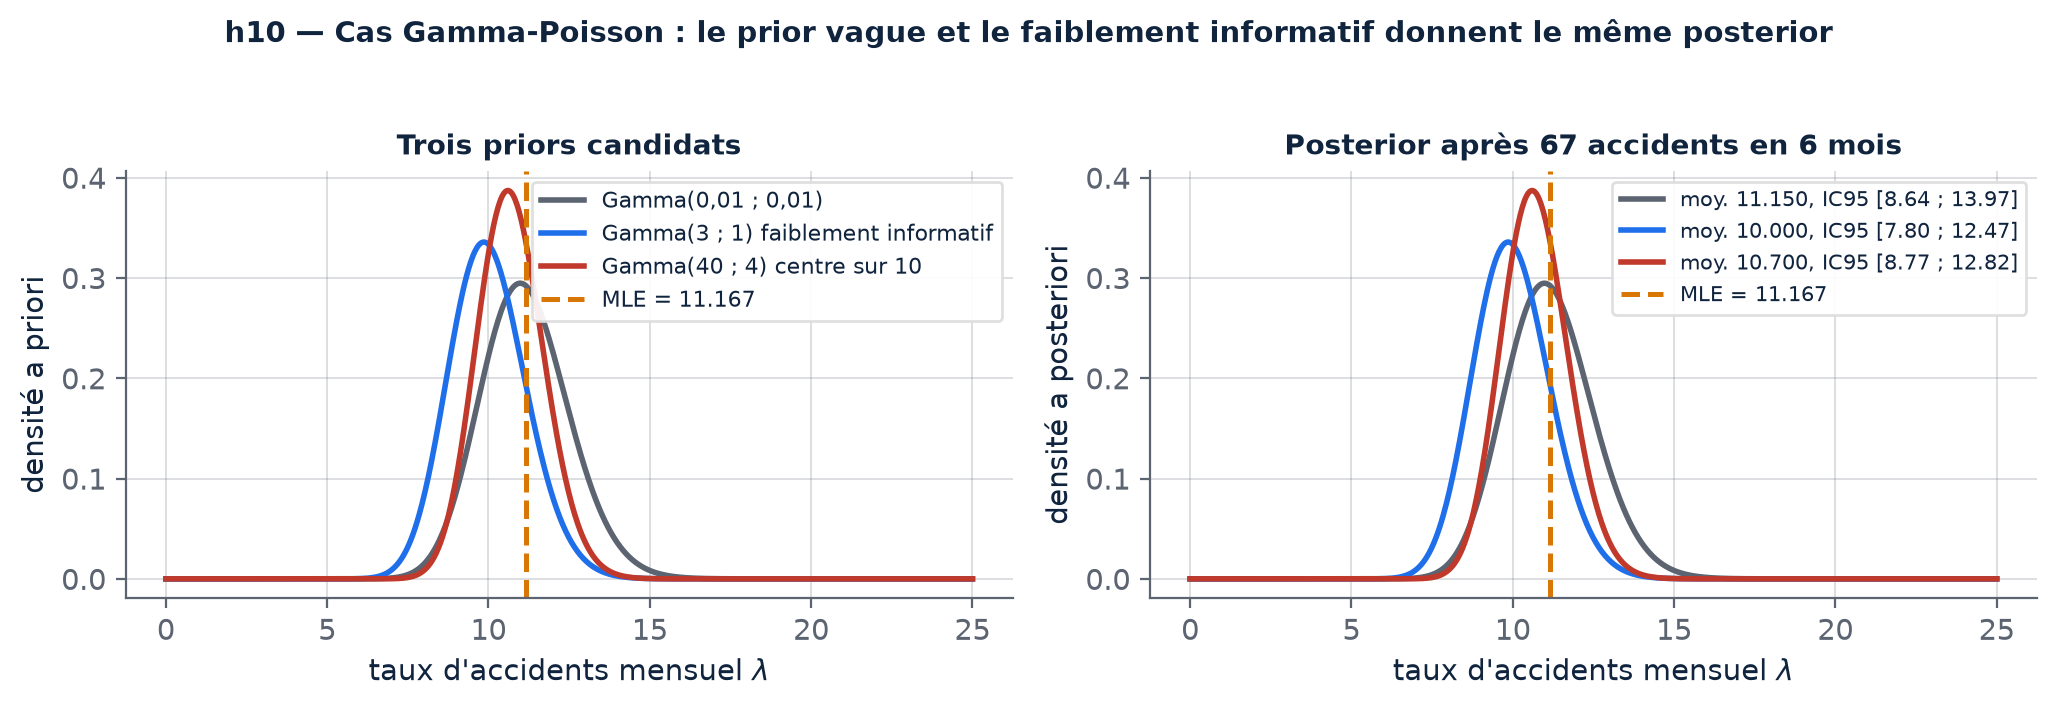
\includegraphics[width=.88\textwidth]{h10_gamma_poisson.png}
\end{center}
\end{frame}

\begin{frame}{Gamma-Poisson : le prior change-t-il la conclusion ?}
\small
\begin{solbox}[Posterior et crédibilité, calculés]
\footnotesize
\centering
\resizebox{\ifdim\width>\linewidth\linewidth\else\width\fi}{!}{%
\begin{tabular}{@{}lccc@{}}
\toprule
Prior & moyenne & IC $95\,\%$ & largeur \\
\midrule
Gamma$(0{,}01\,;0{,}01)$ & $11{,}150$ & $[8{,}64\,;13{,}97]$ & $5{,}332$ \\
Gamma$(3\,;1)$ & $10{,}000$ & $[7{,}80\,;12{,}48]$ & $4{,}679$ \\
Gamma$(40\,;4)$ & $10{,}700$ & $[8{,}77\,;12{,}82]$ & $4{,}052$ \\
\midrule
\multicolumn{4}{@{}l@{}}{\textbf{MLE} : $11{,}167$} \\
\bottomrule
\end{tabular}}
\vspace{1.5mm}

$P(\lambda > 12 \given y)$ : $0{,}258$ (prior vague) contre $0{,}107$ (prior fort).
\end{solbox}
\vspace{1mm}
\begin{columns}[t]
\begin{column}{0.49\textwidth}
\begin{kbox}[Leçon 1 : les données dominent]
Le prior vague et le prior faiblement informatif donnent la \emph{même} réponse à
$1\,\%$ près : avec $67$ événements, la vraisemblance écrase toute croyance molle.
\end{kbox}
\end{column}
\begin{column}{0.49\textwidth}
\begin{kbox}[Leçon 2 : un prior fort engage]
Avec Gamma$(40\,;4)$ --- un site \emph{a priori} sûr --- la probabilité de franchir
le seuil tombe de $26\,\%$ à $11\,\%$. Un prior fort doit être \textbf{documenté}.
\end{kbox}
\end{column}
\end{columns}
\end{frame}

% ---------------------------------------------------------------- 37
\begin{frame}{Section 3.4 --- Cas appliqué 2 : Normal-Normal (mesures répétées)}
\small
\vspace{-1.5mm}
\begin{columns}[t]
\begin{column}{0.53\textwidth}
\begin{ebox}[Énoncé : pesée d'un lot de poudre]
Sept mesures ont été faites sur le même échantillon :
\[
y = (112,\ 121,\ 108,\ 117,\ 126,\ 115,\ 119)\ \mathrm{g},\qquad
\bar y = 116{,}857 .
\]
On connaît le bruit de la balance : $\sigma = 8$ g. Le vrai poids moyen suit un
prior $\mathcal{N}(\mu_0, \tau_0^2)$ avec $\mu_0 = 100$, $\tau_0 = 15$.
\end{ebox}
\begin{kbox}[Conjugaison par les \textbf{précisions}]
\vspace{-1mm}
\[
\frac{1}{\sigma_{\text{post}}^2} = \frac{1}{\tau_0^2} + \frac{n}{\sigma^2},
\qquad
\mu_{\text{post}} = \sigma_{\text{post}}^2\left(\frac{\mu_0}{\tau_0^2} + \frac{n\bar y}{\sigma^2}\right)
\]
\end{kbox}
\end{column}
\begin{column}{0.45\textwidth}
\begin{solbox}[Calcul exécuté]
{\footnotesize
$\frac{1}{\sigma_{\text{post}}^2} = \frac{1}{225} + \frac{7}{64} = 0{,}11382$
\[
\Rightarrow\; \sigma_{\text{post}} = 2{,}964, \quad \mu_{\text{post}} = 116{,}199
\]
crédibilité $95\,\%$ : $[110{,}39\,;122{,}01]$
}
\vspace{1mm}
\footnotesize L'écart-type a posteriori ($2{,}96$) est à peine inférieur à celui
de la moyenne des mesures $\sigma/\sqrt n = 3{,}02$ : la réduction vaut
$1{,}97\,\%$ seulement. Le prior, ici, \textbf{n'apporte presque rien}.
\end{solbox}
\end{column}
\end{columns}
\vspace{1mm}
\begin{tcolorbox}[colback=byLight,colframe=byGrey!55,arc=2mm,width=.95\textwidth]
\centering\small
\textbf{Le réflexe à acquérir} : comparer $\sigma_{\text{post}}$ à $\sigma/\sqrt n$.
Si le prior améliorait vraiment, on verrait $\sigma_{\text{post}} \ll \sigma/\sqrt n$.
Dans cet exemple, $7$ mesures valent plus que l'expert.
\end{tcolorbox}
\end{frame}

% ---------------------------------------------------------------- 38
\begin{frame}{Normal-Normal : mise à jour et prédiction de la prochaine mesure}
\small
\vspace{-2mm}
\begin{center}
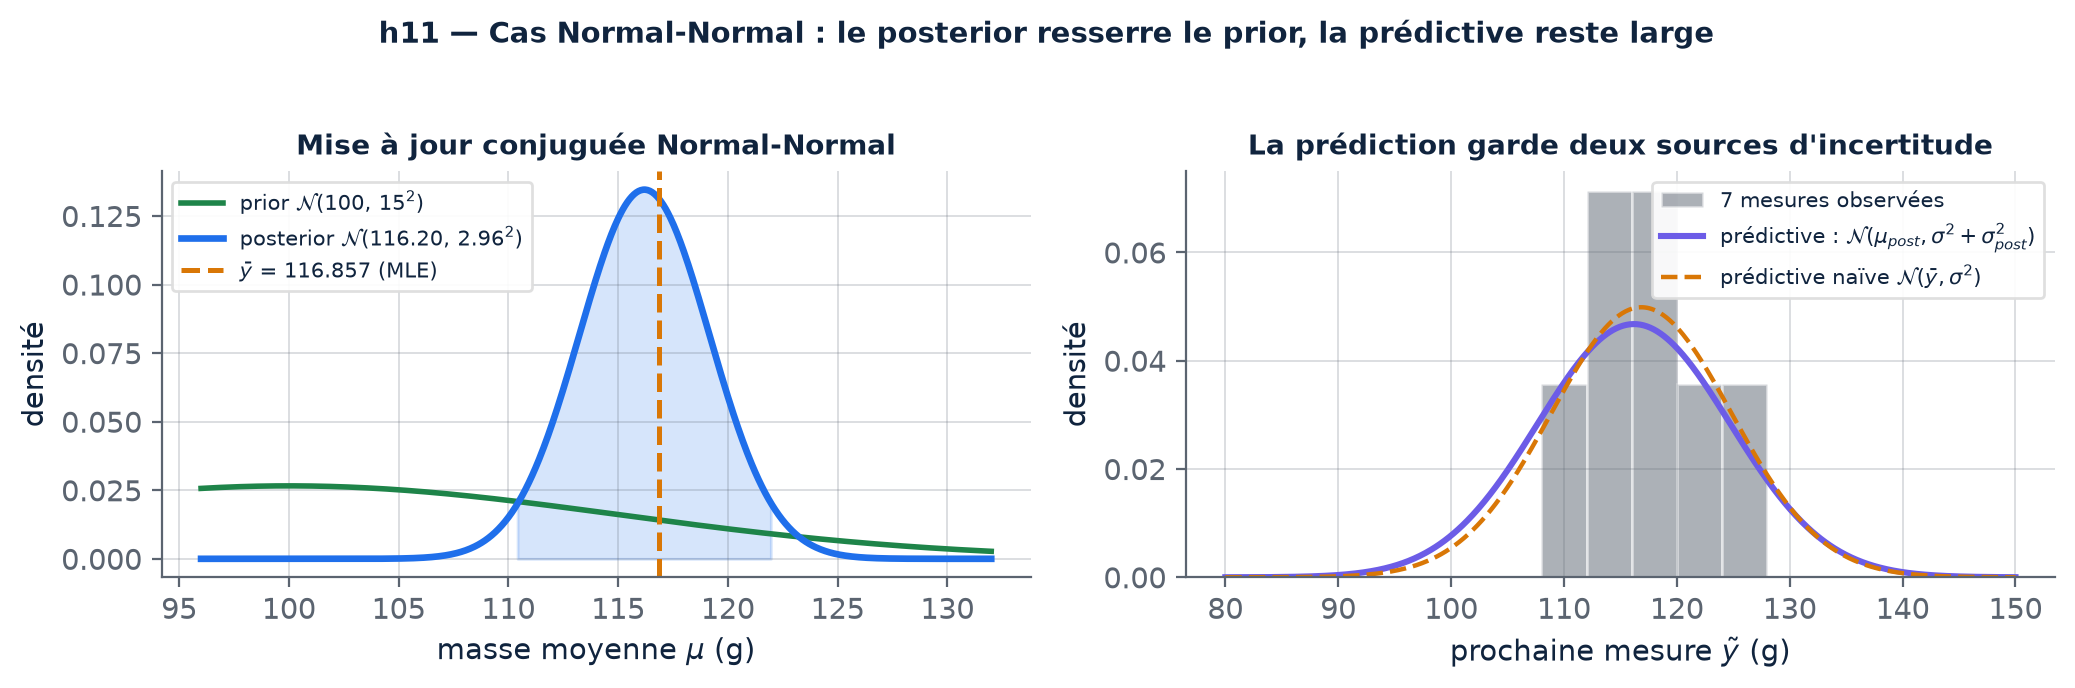
\includegraphics[width=.74\textwidth]{h11_normal_normal.png}
\end{center}
\vspace{-1.5mm}
\begin{columns}[t]
\begin{column}{0.56\textwidth}
\begin{ebox}[Les deux panneaux, lus dans le bon ordre]
À gauche : le prior $\mathcal{N}(100, 15^2)$ se resserre en
$\mathcal{N}(116{,}20\,; 2{,}96^2)$ autour de $\bar y = 116{,}86$.
À droite : la prédiction de la \emph{prochaine} mesure garde l'incertitude de
mesure, donc elle reste large.
\end{ebox}
\end{column}
\begin{column}{0.42\textwidth}
\begin{solbox}[Écart-type prédictif]
{\footnotesize
\[
\sigma_{\text{pred}} = \sqrt{\sigma^2 + \sigma_{\text{post}}^2} = \sqrt{64 + 8{,}79}
\]
\[
= \mathbf{8{,}53}
\]
}
Intervalle prédictif $95\,\%$ : $[99{,}48\,;132{,}92]$, de largeur $33{,}44$
--- contre $31{,}36$ pour l'approche naïve. \textbf{La différence est le prix
de l'honnêteté.}
\end{solbox}
\end{column}
\end{columns}
\end{frame}

% ---------------------------------------------------------------- 39
\begin{frame}[fragile]{Régression linéaire bayésienne complète en PyMC}
\footnotesize
\vspace{-2.5mm}
\begin{codebox}[Modèle, échantillonnage et résumé --- code réellement exécuté]
\begin{lstlisting}
import numpy as np, pymc as pm, arviz as az
n = 25
x = np.sort(rng.uniform(0.2, 5.0, n))
y = 2.0 + 1.5 * x + rng.normal(0.0, 0.9, n)   # verite : a=2, b=1.5, s=0.9
with pm.Model() as mreg:
    alpha = pm.Normal("alpha", mu=0.0, sigma=5.0)   # priors faiblement informatifs
    beta  = pm.Normal("beta",  mu=0.0, sigma=5.0)
    sigma = pm.HalfNormal("sigma", sigma=2.0)
    mu    = alpha + beta * x
    pm.Normal("y", mu=mu, sigma=sigma, observed=y)  # vraisemblance = modele lineaire
    idata = pm.sample(draws=1000, tune=600, chains=2, cores=1, random_seed=3)
print(az.summary(idata, var_names=["alpha", "beta", "sigma"]))  # R-hat, ESS, moyennes
\end{lstlisting}
\end{codebox}
\vspace{0.5mm}
\begin{columns}[t]
\begin{column}{0.56\textwidth}
\begin{kbox}[Pourquoi ces priors ?]
$\mathcal{N}(0, 5^2)$ laisse $\alpha$ et $\beta$ parcourir $\pm 10$ : c'est
\textbf{informations nulles}. Un $\mathcal{HalfNormal}(2)$ sur $\sigma$ interdit
les variabilités absurdes sans fixer l'échelle : le prior doit se \emph{voir}
sans se \emph{sentir}.
\end{kbox}
\end{column}
\begin{column}{0.42\textwidth}
\begin{solbox}[Coût réel de l'exécution]
\begin{itemize}
  \item $2$ chaînes $\times$ $1\,000$ tirages $= 2\,000$ échantillons, en $348$ s
        sur CPU (sans compilateur C ni GPU) ;
  \item $\hat R$ max $= 1{,}0034$, ESS min $= 908$, $0$ divergence.
\end{itemize}
\end{solbox}
\end{column}
\end{columns}
\end{frame}

% ---------------------------------------------------------------- 40
\begin{frame}{Posterior des coefficients : nuage, bandes et posterior joint}
\small
\vspace{-1.5mm}
\begin{center}
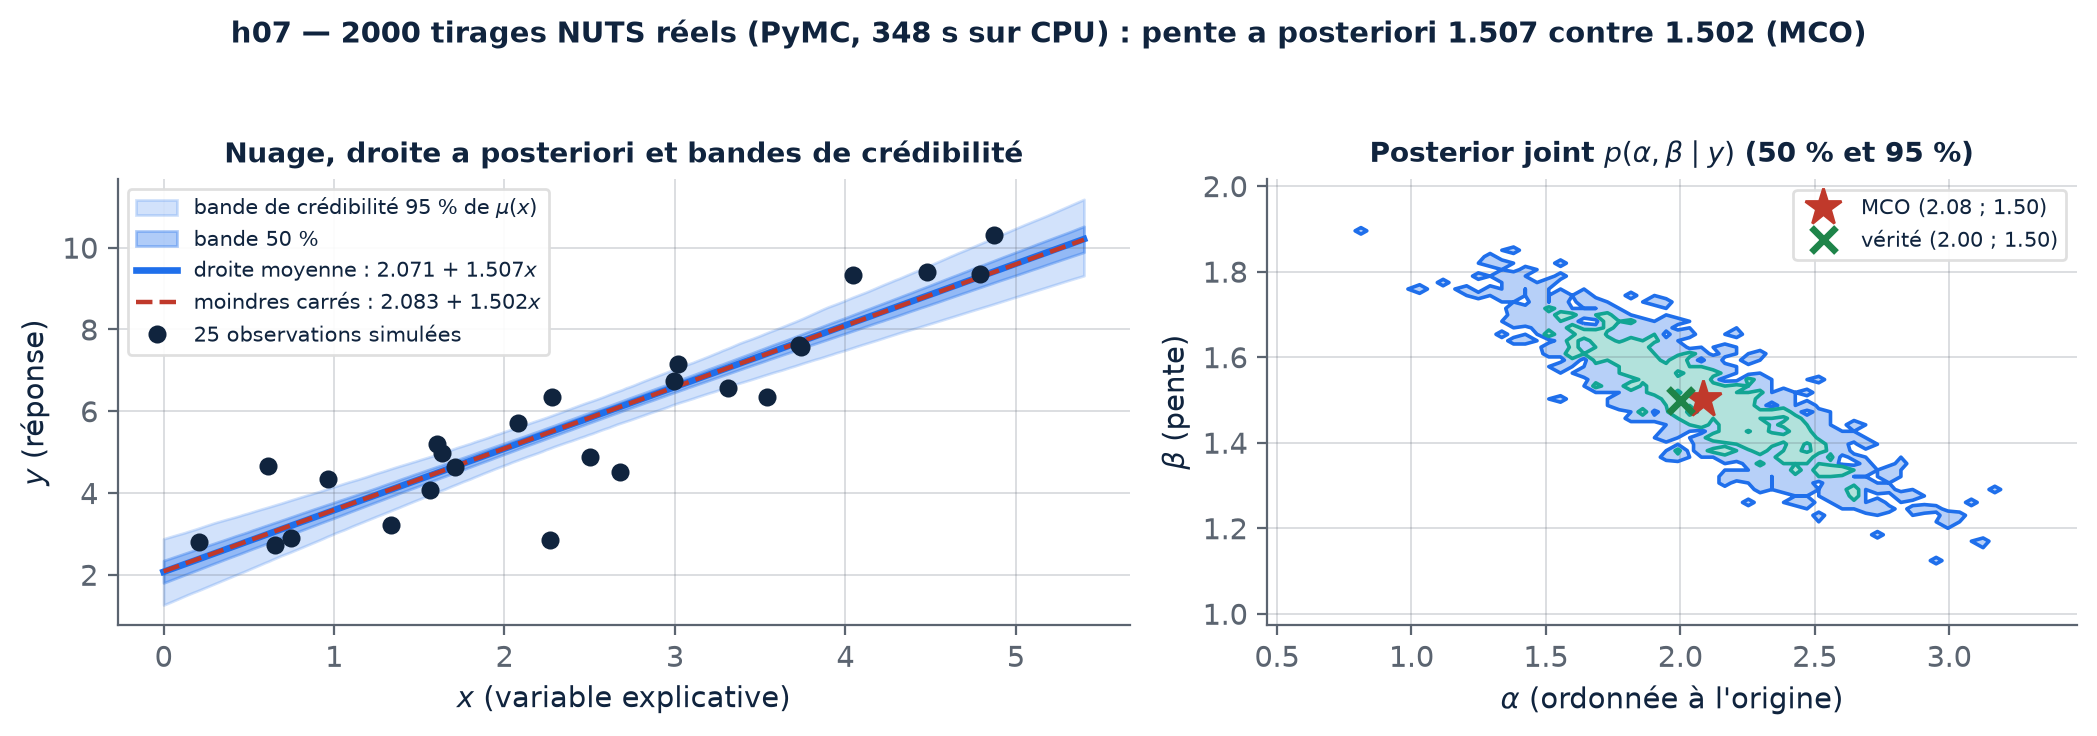
\includegraphics[width=.76\textwidth]{h07_regression_bayesienne.png}
\end{center}
\vspace{-1.5mm}
\begin{columns}[t]
\begin{column}{0.54\textwidth}
\begin{ebox}[Trois colonnes, trois lectures]
À gauche : nuage, droite moyenne et bandes de crédibilité $50\,\%$ et $95\,\%$
de $\mu(x)$. Au centre : le posterior \textbf{joint} $p(\alpha, \beta \given y)$.
À droite : la pente, indiscernable des MCO.
\end{ebox}
\end{column}
\begin{column}{0.44\textwidth}
\begin{solbox}[Chiffres de l'échantillonnage]
\resizebox{\ifdim\width>\linewidth\linewidth\else\width\fi}{!}{%
\begin{tabular}{@{}lccc@{}}
\toprule
Paramètre & MCO & Bayes & vérité \\
\midrule
$\alpha$ & $2{,}083$ & $2{,}071$ & $2{,}00$ \\
$\beta$  & $1{,}502$ & $1{,}507$ & $1{,}50$ \\
$\sigma$ & ---      & $0{,}995$ & $0{,}90$ \\
\bottomrule
\end{tabular}}
\vspace{1.5mm}

HDI $95\,\%$ de $\beta$ : $[1{,}236\,;1{,}797]$ (contient $1{,}5$) ;
$P(\beta > 1 \given y) = 0{,}9995$.
\end{solbox}
\end{column}
\end{columns}
\end{frame}

% ---------------------------------------------------------------- 41
\begin{frame}{Diagnostics MCMC réels : peut-on croire ces tirages ?}
\small
\vspace{-1.5mm}
\begin{center}
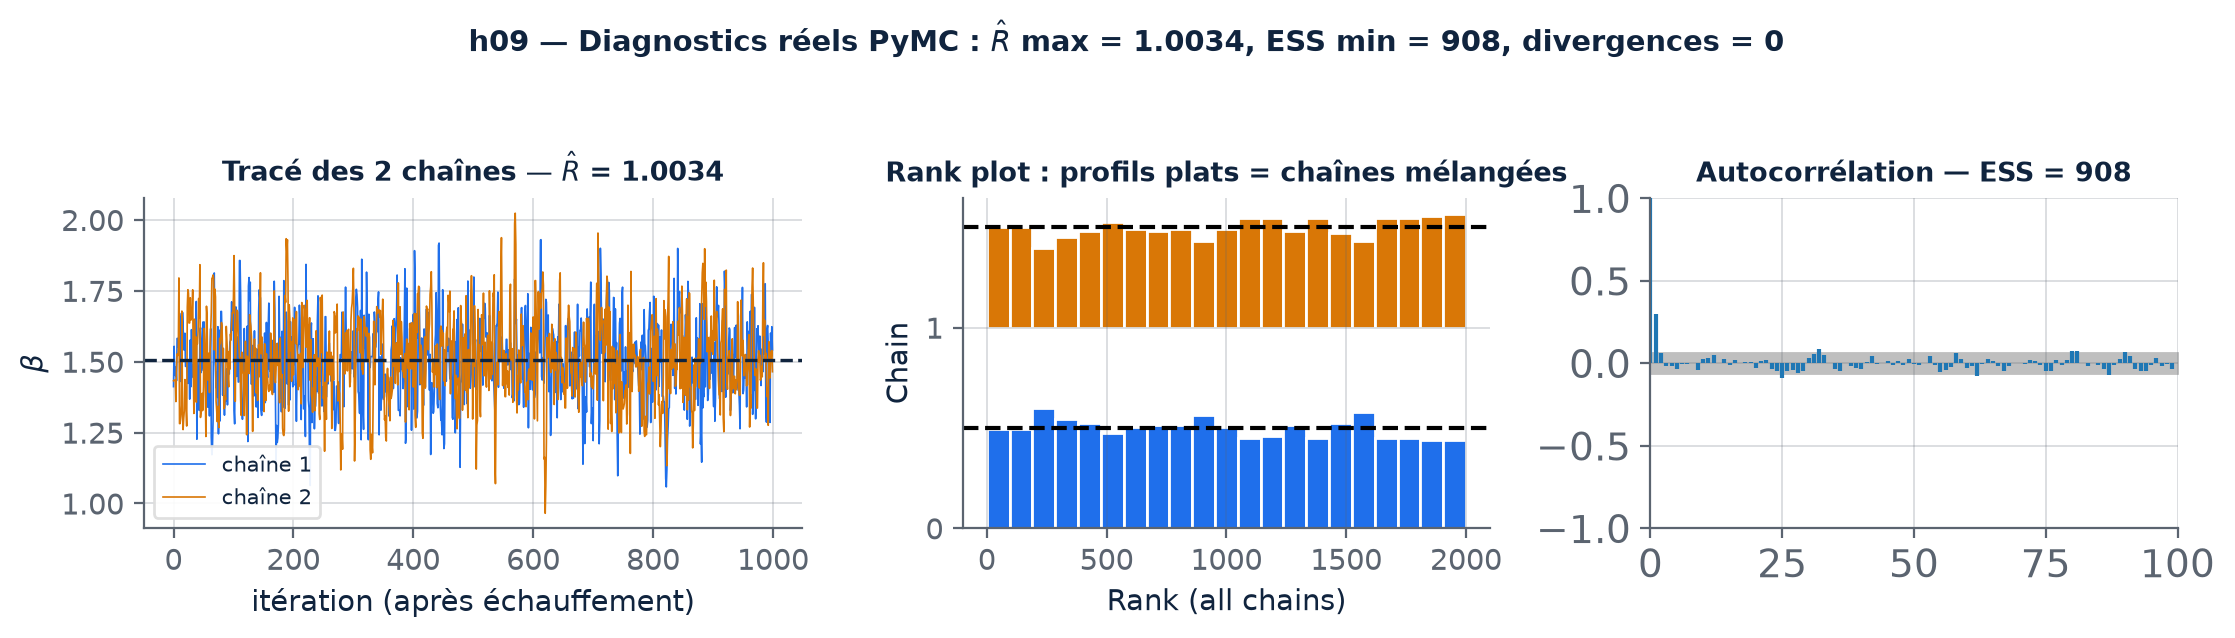
\includegraphics[width=.84\textwidth]{h09_pymc_trace.png}
\end{center}
\vspace{-1.5mm}
\begin{columns}[t]
\begin{column}{0.55\textwidth}
\begin{ebox}[Le trio de contrôle, valeurs lues sur cette exécution]
\begin{tabular}{@{}lccc@{}}
\toprule
Paramètre & $\hat R$ & ESS & divergences \\
\midrule
$\alpha$ & $1{,}0034$ & $918{,}0$ & $0$ \\
$\beta$  & $1{,}0024$ & $907{,}9$ & $0$ \\
$\sigma$ & $1{,}0022$ & $1\,043{,}0$ & $0$ \\
\bottomrule
\end{tabular}
\vspace{1mm}
\footnotesize $\hat R$ proche de $1$ et ESS élevé : les deux chaînes explorent la
même loi. Un tracé « en chenille » sans dérive et un rank plot plat confirment
visuellement ce que les nombres disent.
\end{ebox}
\end{column}
\begin{column}{0.43\textwidth}
\begin{kbox}[Seuils usuels à retenir]
\begin{itemize}
  \item $\hat R < 1{,}01$ (idéalement $< 1{,}005$) ;
  \item $\mathrm{ESS} > 400$ par paramètre ;
  \item $0$ divergence, $0$ message d'avertissement ;
  \item sinon : augmenter \py{tune}, reparamétrer (centrer $x$), ou changer de prior.
\end{itemize}
\end{kbox}
\end{column}
\end{columns}
\end{frame}

% ---------------------------------------------------------------- 42
\begin{frame}{Densités marginales et deux notions d'intervalle}
\small
\vspace{-2mm}
\begin{center}
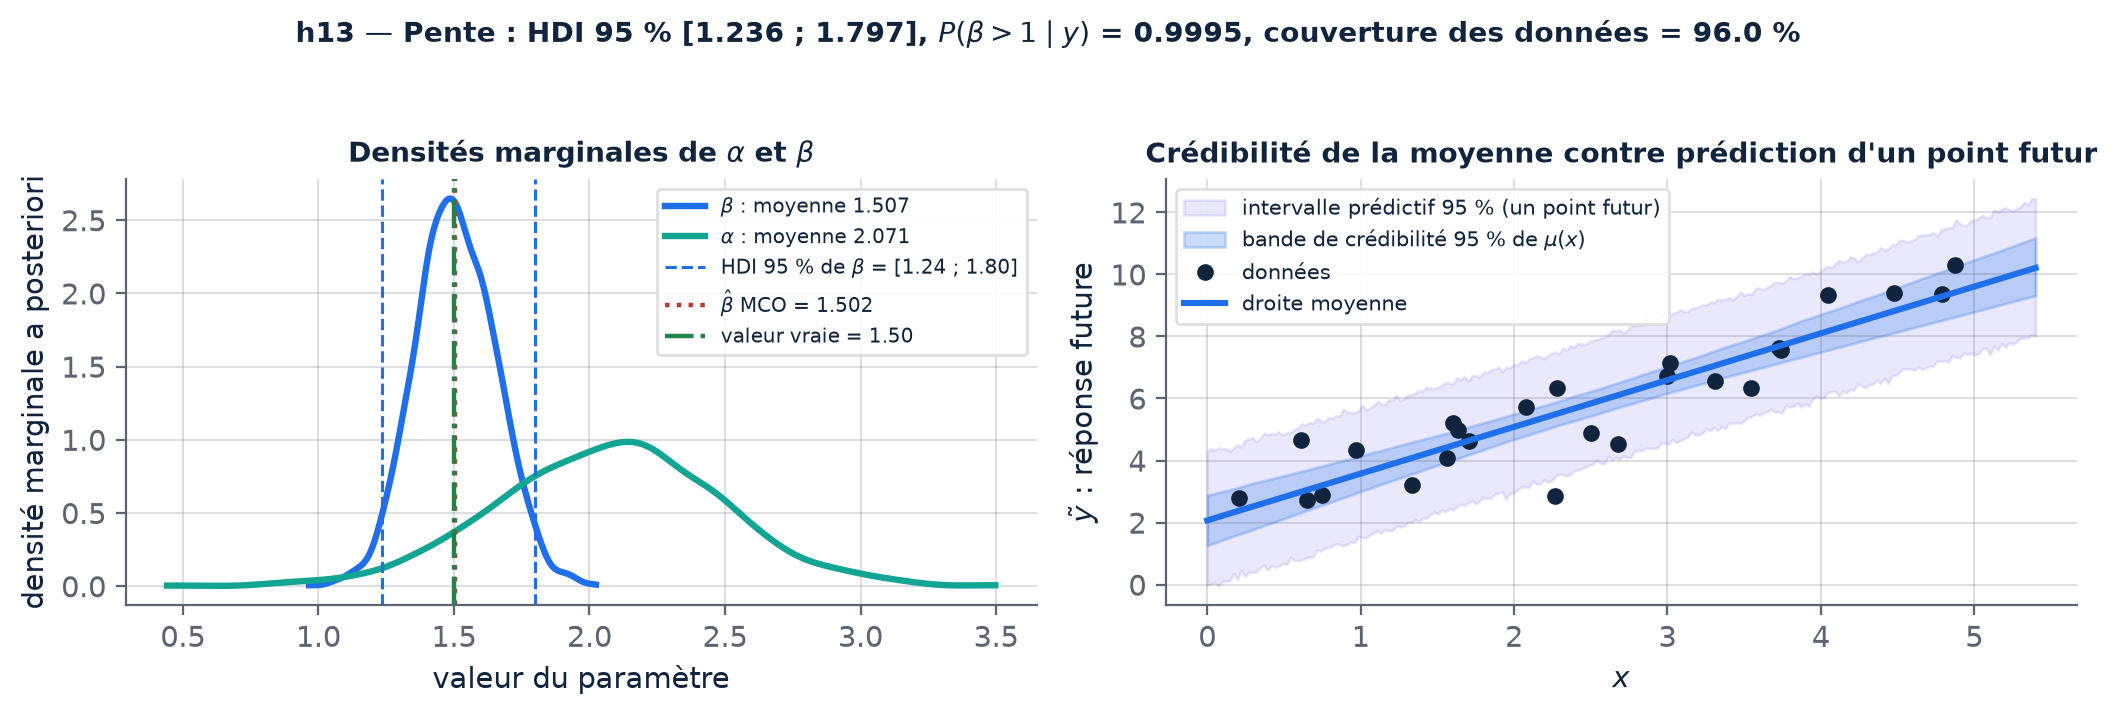
\includegraphics[width=.72\textwidth]{h13_regression_marginales.png}
\end{center}
\vspace{-1.5mm}
\begin{columns}[t]
\begin{column}{0.55\textwidth}
\begin{ebox}[Ce que la figure sépare nettement]
À gauche : les densités marginales de $\alpha$ et $\beta$ ; l'HDI $95\,\%$ de
$\beta$, $[1{,}236\,;1{,}797]$, \textbf{couvre} la valeur vraie $1{,}5$, et la
pente MCO ($1{,}502$) tombe au centre.
À droite : la \textbf{bande de crédibilité} de $\mu(x)$ (étroite) et
l'\textbf{intervalle prédictif} d'une observation future (large) --- deux
questions différentes.
\end{ebox}
\end{column}
\begin{column}{0.43\textwidth}
\begin{solbox}[Contrôle prédictif exécuté]
Sur les $25$ observations, $96\,\%$ (soit $24/25$) tombent dans l'intervalle
prédictif à $95\,\%$ : conforme à l'attendu, le modèle reproduit les données
observées.
\end{solbox}
\begin{kbox}[Phrase à écrire dans un rapport]
« La pente vaut $1{,}51$, intervalle de crédibilité $95\,\%$
$[1{,}24\,;1{,}80]$ » : jamais « $\pm$ ».
\end{kbox}
\end{column}
\end{columns}
\end{frame}

% ---------------------------------------------------------------- 43
\begin{frame}{Bande de crédibilité contre intervalle de prédiction}
\begin{columns}[t]
\begin{column}{0.49\textwidth}
\begin{tcolorbox}[enhanced,colback=byBlue!6,colframe=byBlue,arc=2mm,
   title={\bfseries\color{white} Bande de crédibilité de $\mu(x)$},colbacktitle=byBlue,
   attach boxed title to top left={xshift=3mm,yshift=-2mm},
   boxed title style={arc=1mm,boxrule=0pt}]
\begin{itemize}
  \item Question : « où se situe la \textbf{moyenne} du processus ? »
  \item Se resserre comme $1/\sqrt n$ et peut devenir très étroite.
  \item Utile pour comparer des groupes, tester un effet, communiquer une
        estimation.
\end{itemize}
\end{tcolorbox}
\end{column}
\begin{column}{0.49\textwidth}
\begin{tcolorbox}[enhanced,colback=byPurple!7,colframe=byPurple,arc=2mm,
   title={\bfseries\color{white} Intervalle de prédiction de $\tilde y$},colbacktitle=byPurple,
   attach boxed title to top left={xshift=3mm,yshift=-2mm},
   boxed title style={arc=1mm,boxrule=0pt}]
\begin{itemize}
  \item Question : « quelle valeur \textbf{individuelle} vais-je observer ? »
  \item Ne descend \textbf{jamais} sous le bruit intrinsèque $\sigma$ :
        largeur $\geq 2 \times 1{,}96\,\sigma$.
  \item Utile pour dimensionner, garantir, alerter.
\end{itemize}
\end{tcolorbox}
\end{column}
\end{columns}
\vspace{1mm}
\begin{wbox}[La confusion la plus coûteuse en pratique]
\small Annoncer la bande de crédibilité de la \emph{moyenne} comme une garantie sur
les \emph{individus}. Sur l'exemple de la balance : la moyenne est connue à
$\pm 5{,}8$ g ($95\,\%$), mais chaque pesée future peut s'écarter de $\pm 16{,}7$ g.
Confondre les deux, c'est promettre au client une tolérance
\textbf{deux fois} trop serrée.
\end{wbox}
\end{frame}

% ---------------------------------------------------------------- 44
% [split]
\begin{frame}{Risque MSE : estimateur bayésien contre maximum de vraisemblance}
\begin{center}
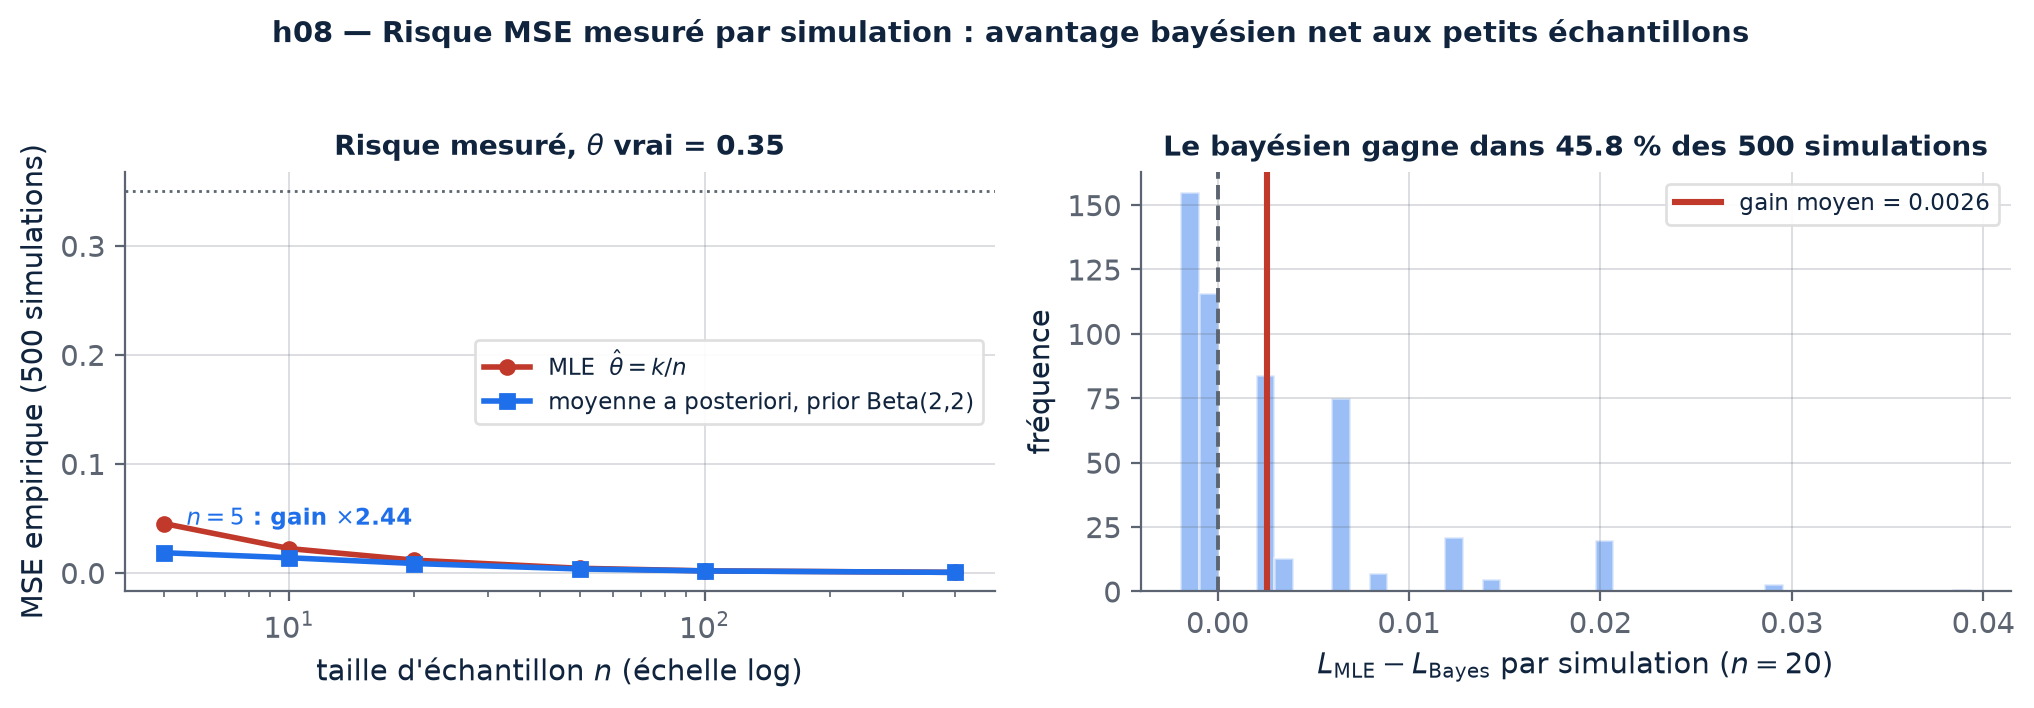
\includegraphics[width=.86\textwidth]{h08_mse_bayes_vs_mle.png}
\end{center}
\end{frame}

% [split]
\begin{frame}{Risque MSE : estimateur bayésien contre maximum de vraisemblance}
\small
\vspace{-2mm}

\vspace{-1.5mm}
\begin{columns}[t]
\begin{column}{0.56\textwidth}
\begin{ebox}[Protocole : 500 simulations réelles]
$\theta_{\text{vrai}} = 0{,}35$ ; pour chaque $n \in \{5, 10, 20, 50, 100, 400\}$,
on simule $500$ jeux de données, on calcule
$\hat\theta_{\text{MLE}} = k/n$ et
$\hat\theta_{\text{Bayes}} = (k+2)/(n+4)$ (prior Beta$(2,2)$), puis le MSE
empirique. Aucune formule asymptotique n'est invoquée : on \emph{mesure}.
\end{ebox}
\end{column}
\begin{column}{0.42\textwidth}
\begin{solbox}[Résultats mesurés]
\footnotesize
\resizebox{\ifdim\width>\linewidth\linewidth\else\width\fi}{!}{%
\begin{tabular}{@{}lccc@{}}
\toprule
$n$ & MSE MLE & MSE Bayes & rapport \\
\midrule
$5$ & $0{,}04526$ & $0{,}01853$ & $\mathbf{0{,}41}$ \\
$20$ & --- & --- & $0{,}74$ \\
$400$ & $0{,}000518$ & $0{,}000518$ & $1{,}00$ \\
\bottomrule
\end{tabular}}
\vspace{1.5mm}

Gain moyen à $n = 20$ : $0{,}00259$, positif dans $45{,}8\,\%$ des $500$ simulations.
\end{solbox}
\end{column}
\end{columns}
\vspace{1mm}
\begin{kbox}[Comment lire la variabilité du gain]
Le gain est positif \emph{en moyenne} mais pas à chaque tirage : un estimateur
rétréci peut perdre sur un échantillon particulier. C'est le prix de
l'amélioration en risque --- et la raison pour laquelle on recommande le bayésien
pour des \textbf{problèmes répétés}, pas pour un cas unique.
\end{kbox}
\end{frame}

% ---------------------------------------------------------------- 45
\begin{frame}{Atelier --- du modèle à la décision (TP noté, 30 min)}
\footnotesize
\vspace{-2mm}
\begin{abox}[Énoncé du TP]
On dispose d'un jeu de données réel (prix de logements, $n = 200$). On demande :
\begin{enumerate}
  \item Écrire le modèle de régression bayésien en PyMC (priors faiblement
        informatifs sur $\alpha$, $\beta$, $\sigma$).
  \item Échantillonner avec \py{pm.sample()} et vérifier $\hat R < 1{,}01$ et
        $\mathrm{ESS} > 400$.
  \item Produire le nuage + la droite a posteriori + les bandes $50\,\%$ et
        $95\,\%$.
  \item Rapporter l'effet mesuré : moyenne, HDI $95\,\%$, $P(\beta > 0 \given y)$.
  \item Conclure en \textbf{une phrase de décision} pour un agent immobilier :
        « chaque m\textsuperscript{2} supplémentaire vaut X, avec un intervalle
        de [\ldots] ».
\end{enumerate}
\end{abox}
\vspace{1mm}
\begin{columns}[t]
\begin{column}{0.49\textwidth}
\begin{kbox}[Grille d'évaluation]
4 pts modèle correct ; 2 pts diagnostics affichés ; 4 pts figure lisible avec
légende ; 6 pts interprétation (estimateur choisi et perte justifiée) ;
4 pts qualité du code (reproductible, \py{random_seed} fixé).
\end{kbox}
\end{column}
\begin{column}{0.49\textwidth}
\begin{qbox}[Question de contrôle]
Un étudiant annonce « $\beta = 1200$~euros/m\textsuperscript{2}, intervalle de
crédibilité $[900\,;1500]$ ». Que manque-t-il à cette phrase pour être
\emph{utilisable} ?
\vspace{1mm}

\textbf{Éléments attendus} : le niveau ($95\,\%$), le type d'intervalle (HDI ou
queues égales), et la précision que c'est l'effet sur la \emph{moyenne}, pas un
intervalle de prédiction pour un logement individuel.
\end{qbox}
\end{column}
\end{columns}
\end{frame}

% ---------------------------------------------------------------- 46
% [suite]
\begin{frame}{Section 3.5 --- Synthèse : du posterior à la décision, en un tableau}
\begin{center}
\small
\begin{tabular}{@{}p{3.3cm}p{3.4cm}p{4.4cm}p{3.2cm}@{}}
\toprule
\textbf{Besoin du commanditaire} & \textbf{Outil bayésien} & \textbf{Sortie chiffrée} & \textbf{Section} \\
\midrule
« Donnez-moi un chiffre » & moyenne / médiane / MAP &
$0{,}300$ / $0{,}286$ / $0{,}250$ sur Beta$(3,7)$ & 3.1 \\
\addlinespace
« Une fourchette crédible » & HDI $95\,\%$ &
$[0{,}080\,;9{,}526]$ sur Gamma$(2\,;0{,}5)$ & 3.2 \\
\addlinespace
« Est-ce au-dessus du seuil ? » & crédibilité unilatérale &
$P(\theta > 0{,}5 \given y) = 0{,}9693$ & 3.2 \\
\addlinespace
« Et si le prior est faux ? » & couverture empirique &
$94{,}6\,\%$ (Wald) contre $23{,}6\,\%$ (prior faux) & 3.2 \\
\addlinespace
« Que va-t-il se passer ? » & prédictive a posteriori &
$P(\tilde y > 6 \given y) = 0{,}1018$ & 3.3 \\
\addlinespace
« Ce modèle tient-il ? » & PPC &
$p_B = 0{,}0073$ : Poisson rejeté & 3.3 \\
\addlinespace
« Quel risque j'accepte ? » & MSE mesuré &
rapport bayésien/MLE $= 0{,}41$ à $n=5$ & 3.4 \\
\bottomrule
\end{tabular}
\end{center}
\vspace{1.5mm}
\end{frame}

% [suite]
\begin{frame}{Section 3.5 --- Synthèse : du posterior à la décision, en un tableau (suite)}
\begin{kbox}[L'arbre de décision du praticien]
Point $\to$ intervalle $\to$ prédiction $\to$ contrôle du modèle. Chaque étape
ajoute une source d'incertitude, donc une raison d'élargir : \textbf{un rapport
bayésien honnête devient de plus en plus large, jamais de plus en plus étroit}.
\end{kbox}
\end{frame}

% ---------------------------------------------------------------- 47
\begin{frame}{Les sept pièges du chapitre 3}
\small
\vspace{-3mm}
\begin{columns}[t]
\begin{column}{0.49\textwidth}
\begin{wbox}[Pièges 1 à 4]
\begin{enumerate}
  \item \textbf{Le point sans perte} : annoncer une moyenne alors que la
        décision paie une perte absolue.
  \item \textbf{Le MAP par réflexe} : non invariant par reparamétrisation, il ne
        doit pas être publié comme « la » réponse.
  \item \textbf{L'intervalle sans étiquette} : HDI ou queues égales ? La largeur
        peut varier de $14\,\%$.
  \item \textbf{La probabilité sur un IC} : « $95\,\%$ de chance que $\theta$ soit
        dans cet IC » n'a pas de sens fréquentiste.
\end{enumerate}
\end{wbox}
\end{column}
\begin{column}{0.49\textwidth}
\begin{wbox}[Pièges 5 à 7]
\begin{enumerate}
  \setcounter{enumi}{4}
  \item \textbf{Le prior oublié} : une couverture de $23{,}6\,\%$ rappelle qu'un
        prior faux produit une assurance fausse.
  \item \textbf{Le point estimé en prédiction} : brancher $\E[\lambda \given y]$
        dans le modèle sous-estime l'intervalle (ici $8{,}53$ contre $8{,}00$
        d'écart-type).
  \item \textbf{Le modèle jamais testé} : sans PPC, une surdispersion de
        $5/30$ dépassements passe inaperçue.
\end{enumerate}
\end{wbox}
\end{column}
\end{columns}
\vspace{1mm}
\begin{kbox}[La règle qui les couvre tous]
Toujours écrire \textbf{la perte, l'intervalle et le modèle} à côté du chiffre.
Un résultat bayésien sans ces trois mentions n'est pas réfutable --- donc pas scientifique.
\end{kbox}
\end{frame}

% ---------------------------------------------------------------- 48
\begin{frame}{Quiz final --- Partie 1 (QCM, 5 questions)}
\begin{qbox}[Cochez la bonne réponse]
\begin{enumerate}
  \item Le mode a posteriori minimise : \; (A) $|\theta-a|$ \; (B) $(\theta-a)^2$
        \; (C) une perte 0--1 \; (D) le MSE.
  \item Sur un posterior Gamma$(2\,;0{,}5)$, le HDI $95\,\%$ est :
        \; (A) plus large \; (B) plus court que l'intervalle à queues égales
        \; (C) identique \; (D) non défini.
  \item Le HDI est faux si le posterior est : \; (A) symétrique \; (B) unimodal
        \; (C) multimodal \; (D) normal.
  \item La loi prédictive a posteriori est : \; (A) plus étroite que la
        vraisemblance au point estimé \; (B) plus large \; (C) identique
        \; (D) toujours normale.
  \item Avec $n_0 = n$, le poids des données dans la moyenne a posteriori
        vaut : \; (A) $0{,}25$ \; (B) $0{,}50$ \; (C) $0{,}67$ \; (D) $1$.
\end{enumerate}
\vspace{1mm}
\textbf{Corrigé} : 1(C) --- 2(B) --- 3(C) --- 4(B) --- 5(B) : le poids vaut
$n/(n+n_0) = 0{,}5$.
\end{qbox}
\end{frame}

% ---------------------------------------------------------------- 49
\begin{frame}{Quiz final --- Partie 2 (exercices, 15 min)}
\footnotesize
\vspace{-2mm}
\begin{qbox}[Exercice 1 --- de la perte à l'estimateur]
Un posterior est Beta$(20,10)$. On paie $L(\theta,a) = 4(a-\theta)$ si $a>\theta$ et
$L(\theta,a)=\theta-a$ si $a<\theta$. Quel quantile faut-il annoncer, et quelle
valeur numérique ?
\vspace{1mm}
\begin{solbox}[Solution --- calculs exécutés]
Le risque a posteriori se dérive en
$\rho'(a) = c_{\text{sur}}P(\theta<a \given y) - c_{\text{sous}}P(\theta>a \given y)$.
Ici $c_{\text{sur}} = 4$ (sur-estimer coûte cher) et
$c_{\text{sous}} = 1$, donc l'optimum vérifie
$P(\theta > a \given y) = \frac{c_{\text{sur}}}{c_{\text{sur}} + c_{\text{sous}}}
= \frac{4}{5}$ : il faut le \textbf{quantile d'ordre $0{,}20$}, et non la médiane
ni un quantile élevé. Sur Beta$(20,10)$ : $q_{0{,}20} = \mathbf{0{,}595}$,
à comparer à la médiane $0{,}670$. Le coût élevé de la sur-estimation
\textbf{tire la recommandation vers le bas}.
\end{solbox}
\end{qbox}
\vspace{1mm}
\begin{columns}[t]
\begin{column}{0.49\textwidth}
\begin{qbox}[Exercice 2 --- diagnostics]
Sur un échantillonnage PyMC réel, on lit $\hat R = 1{,}0034$ pour $\beta$,
$\mathrm{ESS} = 908$ et $0$ divergence. Le résultat est-il exploitable ?
\vspace{1mm}

\textbf{Réponse} : oui. $\hat R < 1{,}01$ et $\mathrm{ESS} > 400$ sont les deux
critères usuels ; $0$ divergence indique que la géométrie du posterior a été
explorée sans difficulté.
\end{qbox}
\end{column}
\begin{column}{0.49\textwidth}
\begin{qbox}[Exercice 3 --- couverture]
Vous obtenez une couverture empirique de $94{,}6\,\%$ avec un IC annoncé à
$95\,\%$ sur $2\,000$ simulations. Est-ce préoccupant ?
\vspace{1mm}

\textbf{Réponse} : sur $2\,000$ répétitions, l'écart type de la couverture vaut
$\sqrt{0{,}95 \times 0{,}05/2000} \approx 0{,}49$ point : l'écart observé est donc
inférieur à un écart type. Non préoccupant.
\end{qbox}
\end{column}
\end{columns}
\end{frame}

% ---------------------------------------------------------------- 50
\begin{frame}{Clôture du chapitre 3 --- cinq messages, une transition}
\footnotesize
\vspace{-2.5mm}
\begin{columns}[t]
\begin{column}{0.55\textwidth}
\begin{kbox}[Les cinq messages à emporter]
\begin{enumerate}
  \item Un estimateur n'existe pas sans \textbf{perte explicitée} :
        quadratique $\to$ moyenne, absolue $\to$ médiane, 0--1 $\to$ mode.
  \item Le \textbf{HDI} est le plus court intervalle de masse donnée ; il peut
        être $14\,\%$ plus étroit que l'intervalle à queues égales.
  \item Un intervalle crédible porte une probabilité sur $\theta$, un IC n'en
        porte pas : la phrase change de sens, pas seulement de notation.
  \item La \textbf{prédictive} est plus large que la vraisemblance au point
        estimé, et le \textbf{PPC} est le seul juge du modèle.
  \item Le risque se \textbf{mesure} : $0{,}41$ fois le MSE du MLE à $n=5$,
        $1{,}00$ à $n=400$.
\end{enumerate}
\end{kbox}
\end{column}
\begin{column}{0.43\textwidth}
\begin{ebox}[Travail demandé]
\begin{itemize}
  \item Refaire la figure h04 avec $n = 5$ puis $n = 100$ : la couverture de
        Wald s'écarte-t-elle encore de $95\,\%$ ?
  \item \textbf{TP3} : \file{notebooks/TP3\_estimation\_\allowbreak prediction\_regression.ipynb}
        — y écrire un PPC pour la régression (points hors bande).
  \item Lire le chapitre 4, section 4.1, avant le cours.
\end{itemize}
\end{ebox}
\begin{tcolorbox}[colback=byCyan!8,colframe=byCyan,arc=2mm]
\centering\small
\textbf{Chapitre 4} : comparer des modèles (facteurs de Bayes, DIC/WAIC) et
décider --- l'estimation est faite, place au \emph{choix}.
\end{tcolorbox}
\end{column}
\end{columns}
\vspace{1mm}
\begin{center}
\small\itshape
« Le posterior ne décide pas à votre place : il vous dit exactement ce que coûte
chaque décision possible. »
\end{center}
\end{frame}

% =====================================================================
%  EPD-SDIA-4112 -- Statistique Bayésienne -- Master 1 SDIA
%  CHAPITRE 4 : Comparaison de modèles et décision   (50 slides, 8 h)
%  Fichier de frames : aucune dépendance à \title (build maître + build seul)
% =====================================================================
\section{Chapitre 4 --- Comparaison et décision}
\chapterslide{Chapitre 4}{Comparaison de modèles et décision}{8 h --- 5 sections --- 50 slides}{%
\textbf{Objectifs} --- quantifier la preuve par un facteur de Bayes et une échelle de
référence ; comparer des modèles hors échantillon (WAIC, LOO) ; choisir une décision qui
minimise le risque a posteriori ; conduire un A/B test sans gonfler le risque ; repérer
les pièges du BF avec un prior vague et du modèle « vrai ».}

% ---------------------------------------------------------------- 1
\begin{frame}{Objectifs pédagogiques du chapitre}
\begin{columns}[t]
\begin{column}{0.48\textwidth}
\begin{kbox}[Savoirs]
\begin{itemize}
  \item Définir le facteur de Bayes et l'interpréter en cotes
  \item Lire l'échelle de Jeffreys sans la surinterpréter
  \item Distinguer le log-score prédictif, le DIC, le WAIC et le LOO
  \item Énoncer la règle de décision qui minimise une perte a posteriori
  \item Historique : le paramètre $\theta$ est fixe (fréquentiste) contre $\theta$ aléatoire (bayésien)
\end{itemize}
\end{kbox}
\end{column}
\begin{column}{0.48\textwidth}
\begin{abox}[Savoir-faire évalués]
\begin{itemize}
  \item Calculer un $BF$ par échantillonnage et par Savage--Dickey
  \item Produire un tableau \py{az.compare()} exploitable
  \item Dériver un seuil de décision à partir d'un rapport de coûts
  \item Construire un intervalle de décision (ROPE) à trois issues
  \item Critiquer un prior (largeur, justification, sensibilité)
\end{itemize}
\end{abox}
\end{column}
\end{columns}
\vspace{1mm}
\begin{tcolorbox}[colback=byLight,colframe=byGrey!50,arc=2mm,width=.95\textwidth]
\centering\small
\textbf{Idée directrice} --- au chapitre 3 on estimait un modèle ; ici on
\textbf{compare des modèles} et on \textbf{transforme une croyance en action}
(accepter, rejeter, traiter, déployer).
\end{tcolorbox}
\end{frame}

% ---------------------------------------------------------------- 2
\begin{frame}{Plan du chapitre 4 (8 h)}
\begin{enumerate}
  \item[4.1] \textbf{Facteur de Bayes} \hfill \textit{slides 5--17}
  \item[4.2] \textbf{Critères hors échantillon} \hfill \textit{slides 18--27}
  \item[4.3] \textbf{Décision bayésienne} \hfill \textit{slides 28--38}
  \item[4.4] \textbf{A/B testing} \hfill \textit{slides 39--46}
  \item[4.5] \textbf{Synthèse, pièges et quiz} \hfill \textit{slides 47--50}
\end{enumerate}
\vspace{2mm}
\begin{tabular}{@{}lrrr@{}}
\toprule
\textbf{Volume} & \textbf{Cours magistral} & \textbf{TD} & \textbf{TP machine} \\
\midrule
8 h & 4 h 30 & 1 h 30 & 2 h \\
\bottomrule
\end{tabular}
\vspace{2mm}
\begin{tcolorbox}[colback=byPurple!6,colframe=byPurple,arc=2mm,width=.95\textwidth]
\small\centering
\textbf{Prérequis mobilisés} : posterior du chapitre 2, HDI et prédictive du chapitre 3,
\py{pymc} et \py{arviz} du chapitre 1, dérivation élémentaire.
\end{tcolorbox}
\end{frame}

% ---------------------------------------------------------------- 3
\begin{frame}{Deux questions que le chapitre 3 laissait ouvertes}
\begin{columns}[t]
\begin{column}{0.47\textwidth}
\begin{ebox}[Question 1 --- le modèle est-il bon ?]
On a estimé $\theta$. Mais \\
est-ce que le modèle $M_1$ (une seule probabilité
pour huit équipes) décrit vraiment les données, comparé à $M_2$
(huit probabilités) ou à $M_3$ (hiérarchique) ?
\vspace{1mm}
\footnotesize Un posterior net ne protège pas d'un modèle faux :
il donne une réponse précise à la mauvaise question.
\end{ebox}
\end{column}
\begin{column}{0.47\textwidth}
\begin{ebox}[Question 2 --- que faire ?]
Un test de dépistage revient positif. Faut-il traiter ? \\
Un bouton B convertit mieux que A sur 2\,000 visites.
Faut-il le déployer à 200\,000 utilisateurs ?
\vspace{1mm}
\footnotesize L'estimation ne décide pas : il faut une
\textbf{fonction de perte} et une règle.
\end{ebox}
\end{column}
\end{columns}
\vspace{1mm}
\begin{kbox}[Les trois réponses du chapitre 4]
\begin{itemize}
  \item \textbf{Facteur de Bayes} : combien de fois les données sont plus plausibles sous $H_0$ que sous $H_1$ ?
  \item \textbf{Critères hors échantillon} : quel modèle prédit le mieux une observation nouvelle ?
  \item \textbf{Décision} : quelle action minimise la perte moyenne a posteriori ?
\end{itemize}
\end{kbox}
\end{frame}

% ---------------------------------------------------------------- 4
% [suite]
\begin{frame}{4.1 Le facteur de Bayes : définition}
% [rogna]
\small
\begin{kbox}[Définition]
Pour deux modèles $M_0$ et $M_1$ munis de leurs priors $\pi_0(\theta_0)$ et $\pi_1(\theta_1)$,
\[
BF_{01} \;=\; \frac{p(y \given M_0)}{p(y \given M_1)}
\;=\; \frac{\displaystyle\int p(y \given \theta_0)\, \pi_0(\theta_0)\,\mathrm{d}\theta_0}
{\displaystyle\int p(y \given \theta_1)\, \pi_1(\theta_1)\,\mathrm{d}\theta_1}
\;=\; \frac{m_0(y)}{m_1(y)} .
\]
$m_k(y)$ est la \textbf{vraisemblance marginale} (ou \textit{évidence}) du modèle $M_k$.
\end{kbox}
\vspace{1mm}
\end{frame}

% [suite]
\begin{frame}{4.1 Le facteur de Bayes : définition (suite)}
\begin{columns}[t]
\begin{column}{0.52\textwidth}
\begin{ebox}[Lecture en cotes]
Les données transforment les cotes a priori en cotes a posteriori :
\[
\underbrace{\frac{P(M_0 \given y)}{P(M_1 \given y)}}_{\text{cotes post.}}
=\underbrace{BF_{01}}_{\text{facteur de Bayes}}\times
\underbrace{\frac{P(M_0)}{P(M_1)}}_{\text{cotes priors}}
\]
Rapport \textbf{multiplicatif}, comme un rapport de cotes en paris.
\end{ebox}
\end{column}
\begin{column}{0.44\textwidth}
\begin{kbox}[Trois propriétés]
\begin{itemize}
  \item \textbf{Symétrie} : $BF_{10} = 1/BF_{01}$
  \item \textbf{Stabilité} : $BF_{01}$ ne dépend pas du plan d'échantillonnage
        (loi de vraisemblance) ni du fait qu'on ait regardé une fois ou dix fois
  \item \textbf{Sensibilité} : $BF_{01}$ \emph{dépend} du prior choisi sous $H_1$
\end{itemize}
\end{kbox}
\end{column}
\end{columns}
\end{frame}

% ---------------------------------------------------------------- 5
% [rogna]
% [rogna]
% [rogna]
% [split]
\begin{frame}{Un rapport de vraisemblances, pas une aire de recouvrement}
\begin{center}
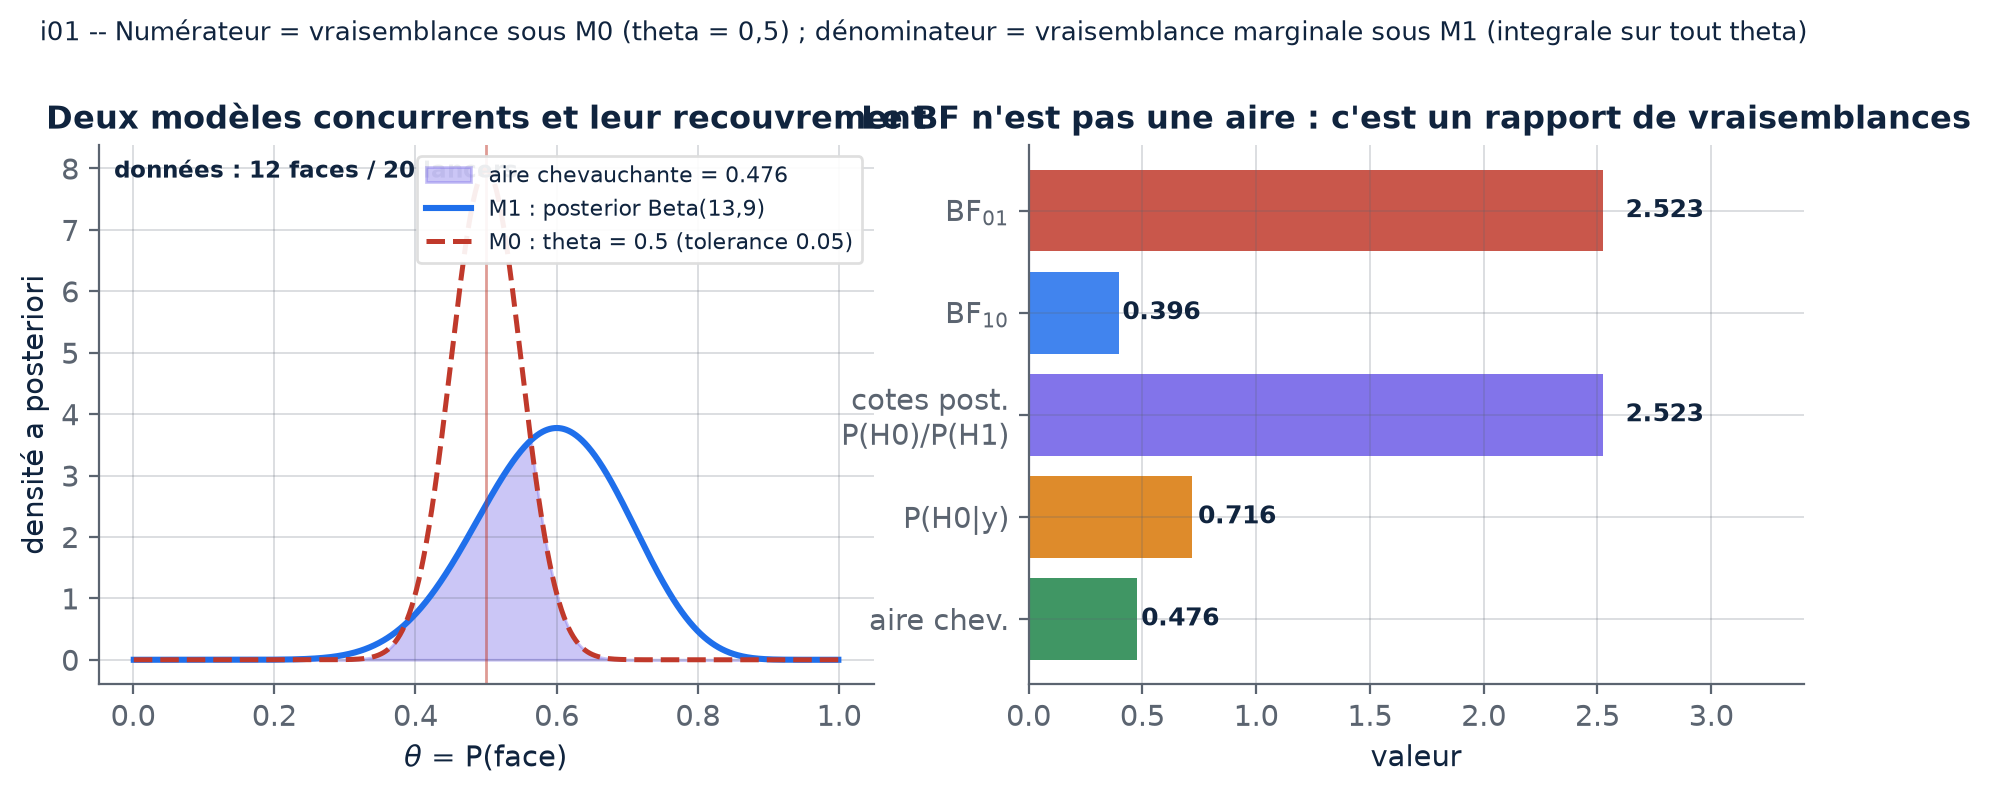
\includegraphics[width=.86\textwidth]{i01_bf_posteriors.png}
\end{center}
\end{frame}

% [split]
\begin{frame}{Un rapport de vraisemblances, pas une aire de recouvrement}

\vspace{-1mm}
\begin{columns}[t]
\begin{column}{0.54\textwidth}
\begin{ebox}[Données --- 12 faces sur 20 lancers (script \file{src/fig\_ch4.py}, exécuté)]
\begin{itemize}
  \item $M_0$ : $\theta = 0{,}5$ exactement ; $M_1$ : $\theta \sim \mathrm{Beta}(1,1)$,
        posterior $\mathrm{Beta}(13,9)$
  \item $BF_{01} = 2{,}523$, $BF_{10} = 0{,}396$ ; cotes postérieures
        (prior 1/2\,--\,1/2) $= 2{,}523$, d'où $P(M_0 \given y) = 0{,}716$
\end{itemize}
\end{ebox}
\end{column}
\begin{column}{0.42\textwidth}
\begin{wbox}[Le piège visuel]
Le recouvrement vaut $0{,}48$ et le $BF$ vaut $2{,}52$ : \textbf{aucun rapport}.
L'aire chevauchante dépend d'une tolérance arbitraire ; le rapport de vraisemblances, non.
{\footnotesize L'aire mesure une \emph{ressemblance de formes} ; le $BF$ mesure
\emph{combien de fois la donnée est plus probable}.}
\end{wbox}
\end{column}
\end{columns}
\end{frame}

% ---------------------------------------------------------------- 6
% [suite]
\begin{frame}[fragile]{Calculer un $BF$ par échantillonnage (Monte-Carlo)}
% [rogna]
\footnotesize
\begin{columns}[t]
\begin{column}{0.53\textwidth}
\begin{codebox}[Monte-Carlo depuis le prior]
\begin{lstlisting}[style=py]
import numpy as np
from math import comb, log
from scipy import special          # betaln

y, n, prior = 12, 20, (1.0, 1.0)

# 1) chemin exact : vraisemblance marginale Beta-Binomiale
lg_m0 = log(comb(n, y)) + n * np.log(0.5)
lg_m1 = (log(comb(n, y))
         + special.betaln(prior[0]+y, prior[1]+n-y)
         - special.betaln(*prior))
bf01_exact = np.exp(lg_m0 - lg_m1)          # 2.5228

# 2) chemin Monte-Carlo : BF10 = E_prior[ p(y|theta)/p(y|theta0) ]
rng  = np.random.default_rng(4112)
th   = rng.random(400_000)                  # theta ~ Beta(1,1)
ratio = (th/0.5)**y * ((1-th)/0.5)**(n-y)
bf10_mc = ratio.mean()                      # 0.39705 +/- 0.00082
bf01_mc = 1 / bf10_mc                       # 2.5185  (err. rel. 0.17 %)
\end{lstlisting}
\end{codebox}
\end{column}
\begin{column}{0.43\textwidth}
\begin{solbox}[Résultat vérifié]
Trois chemins, un seul nombre :
\begin{itemize}
  \item marginale exacte : $BF_{01} = 2{,}5228$
  \item Savage--Dickey : $2{,}5228$ (erreur relative $4\cdot10^{-16}$)
  \item Monte-Carlo (400\,000 tirages) : $2{,}5185 \pm 0{,}0052$
\end{itemize}
\vspace{1mm}
\footnotesize L'estimateur $\widehat{BF}_{10} = \frac1N\sum_i \frac{p(y \given \theta_i)}{p(y \given \theta_0)}$
n'est \emph{pas} un simple rapport de deux vraisemblances : il faut intégrer sur tout
le prior. C'est la différence structurelle avec un rapport de vraisemblance maximal.
\end{solbox}
\end{column}
\end{columns}
\end{frame}

% [suite]
\begin{frame}{Calculer un $BF$ par échantillonnage (Monte-Carlo) (suite)}
\begin{kbox}[Quand c'est instable]
Si le prior $H_1$ est très large devant la région où la vraisemblance vit, l'estimateur
Monte-Carlo a une variance énorme : on préfère alors l'intégration sur grille
(chapitre 5) ou l'échantillonnage d'importance (\py{az.loo}, \py{bridgesampling}).
\end{kbox}

\end{frame}

% ---------------------------------------------------------------- 7
\begin{frame}{Savage--Dickey : le $BF$ d'un point nul sans intégrale}
\begin{columns}[t]
\begin{column}{0.50\textwidth}
\begin{kbox}[Théorème de Savage--Dickey]
Si $H_0$ est un \textbf{point} de $H_1$ ($\theta = \theta_0$ contre $\theta \neq \theta_0$) et si
le prior $\pi_1$ est continu en $\theta_0$, alors l'évidence se lit sur le posterior :
\[
BF_{01} \;=\; \frac{\pi_1(\theta_0 \given y)}{\pi_1(\theta_0)}
\]
Un rapport de \emph{densités} au point nul, pas une intégrale sur l'espace des paramètres.
\end{kbox}
\begin{ebox}[Intuition]
Les données font \textbf{monter} la densité au point nul si $H_0$ est plausible.
$BF_{01} > 1 \iff$ la densité postérieure au point nul dépasse la densité a priori.
\end{ebox}
\end{column}
\begin{column}{0.46\textwidth}
\begin{center}
\begin{figbox}
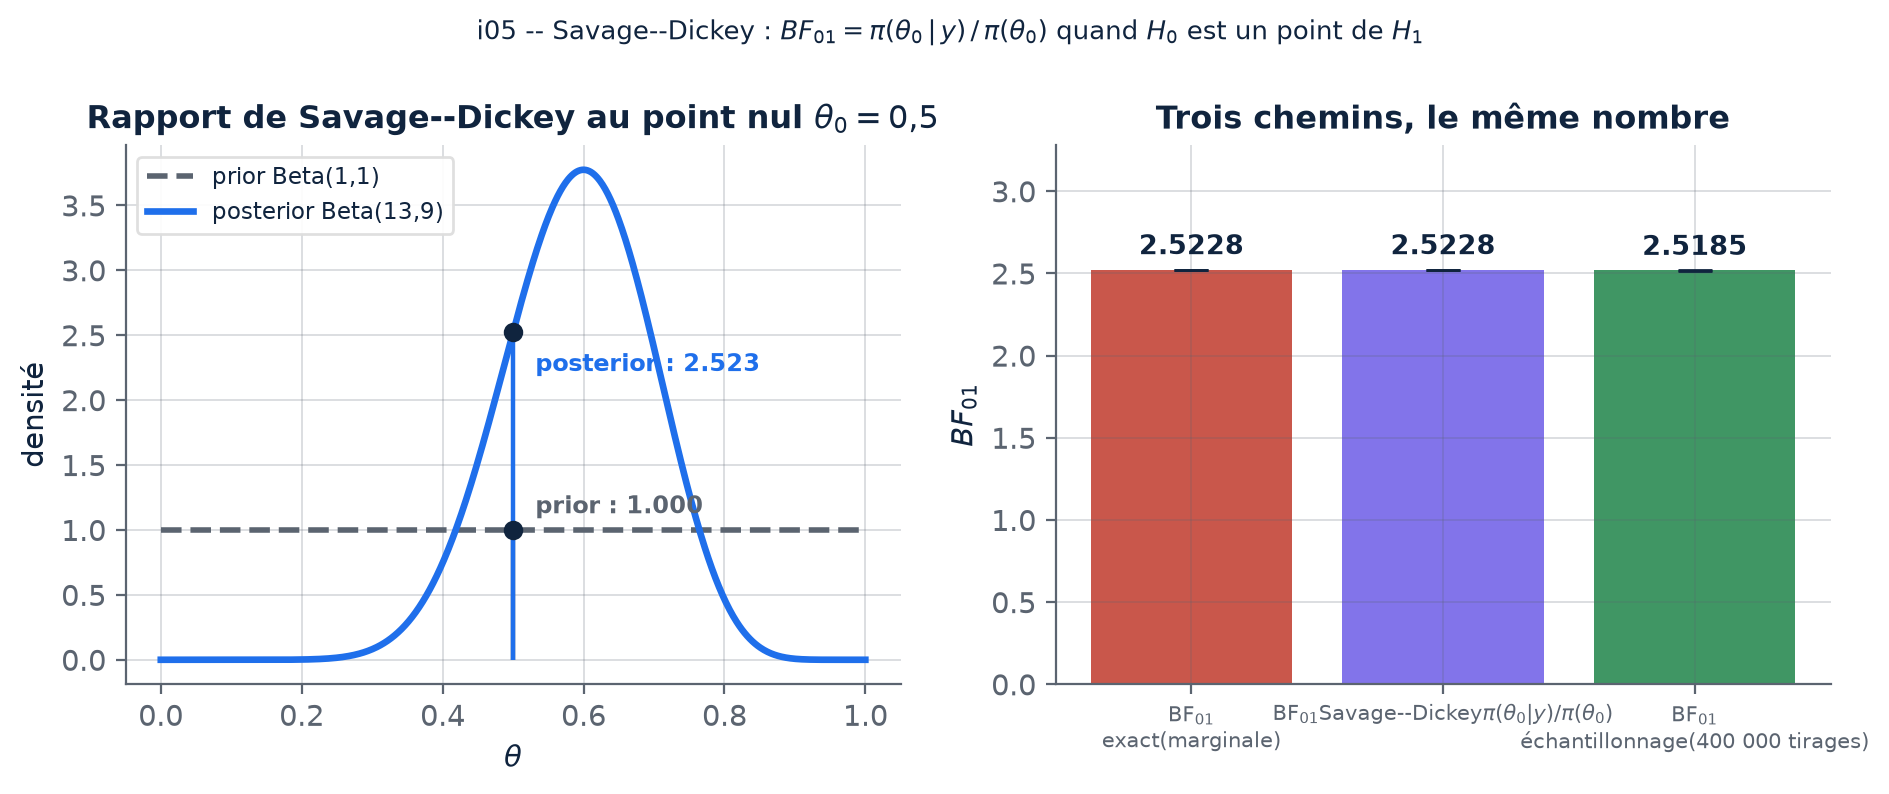
\includegraphics[width=\textwidth]{i05_savage_dickey.png}
\end{figbox}
\end{center}
\begin{solbox}[Vérifié numériquement]
$\pi(0{,}5) = 1{,}0000$ ; $\pi(0{,}5 \given y) = 2{,}5228$ ; $BF_{01} = 2{,}5228$ \\
Monte-Carlo 400\,000 tirages : $2{,}5185 \pm 0{,}0052$ (écart relatif $0{,}17\,\%$).
\end{solbox}
\end{column}
\end{columns}
\end{frame}

% ---------------------------------------------------------------- 8
\begin{frame}{L'échelle de Jeffreys : un vocabulaire, pas une loi}
\begin{center}
\small
\begin{tabular}{@{}p{2.9cm}rrp{6.0cm}@{}}
\toprule
\textbf{Interprétation} & $\log_{10} BF_{01}$ & $BF_{01}$ & \textbf{Usage en TD} \\
\midrule
Anecdotique   & $\vert\log_{10} BF\vert < 0{,}5$ & $< 3{,}2$    & ne rien conclure, collecter plus de données \\
Substantiel   & $0{,}5 \le \log_{10} BF < 1$    & $3{,}2$ à $10$  & présomption seulement \\
Fort          & $1 \le \log_{10} BF < 2$        & $10$ à $100$    & conclusion solide dans le rapport \\
Très fort     & $2 \le \log_{10} BF < 3$        & $100$ à $1\,000$ & conclusion robuste, peu de débat \\
Décisif       & $\log_{10} BF \ge 3$            & $\ge 1\,000$    & basculer la décision, publier \\
\bottomrule
\end{tabular}
\end{center}
\vspace{1mm}
\begin{columns}[t]
\begin{column}{0.47\textwidth}
\begin{kbox}[Ce que l'échelle est]
Une \textbf{convention de lecture} proposée par Jeffreys (1961), reprise par Kass et Raftery (1995).
Elle aide à verbaliser ; elle ne remplace pas un calcul de perte.
\end{kbox}
\end{column}
\begin{column}{0.49\textwidth}
\begin{wbox}[Ce que l'échelle n'est pas]
\begin{itemize}
  \item Ce n'est \textbf{pas} un seuil de significativité : $BF_{01} = 3{,}2$ n'est ni
        « significatif » ni « non significatif ».
  \item Le même $BF$ n'a pas la même importance selon l'enjeu :
        $BF_{01} = 10$ suffit pour un bouton web, jamais pour un essai clinique.
  \item Le facteur $BF_{01}$ n'est pas une probabilité : la probabilité postérieure
        exige des cotes a priori explicites.
\end{itemize}
\end{wbox}
\end{column}
\end{columns}
\end{frame}

% ---------------------------------------------------------------- 9
% [rogna]
% [rogna]
% [rogna]
% [split]
\begin{frame}{Le $BF$ s'accumule : la preuve croît linéairement en $n$}
\begin{center}
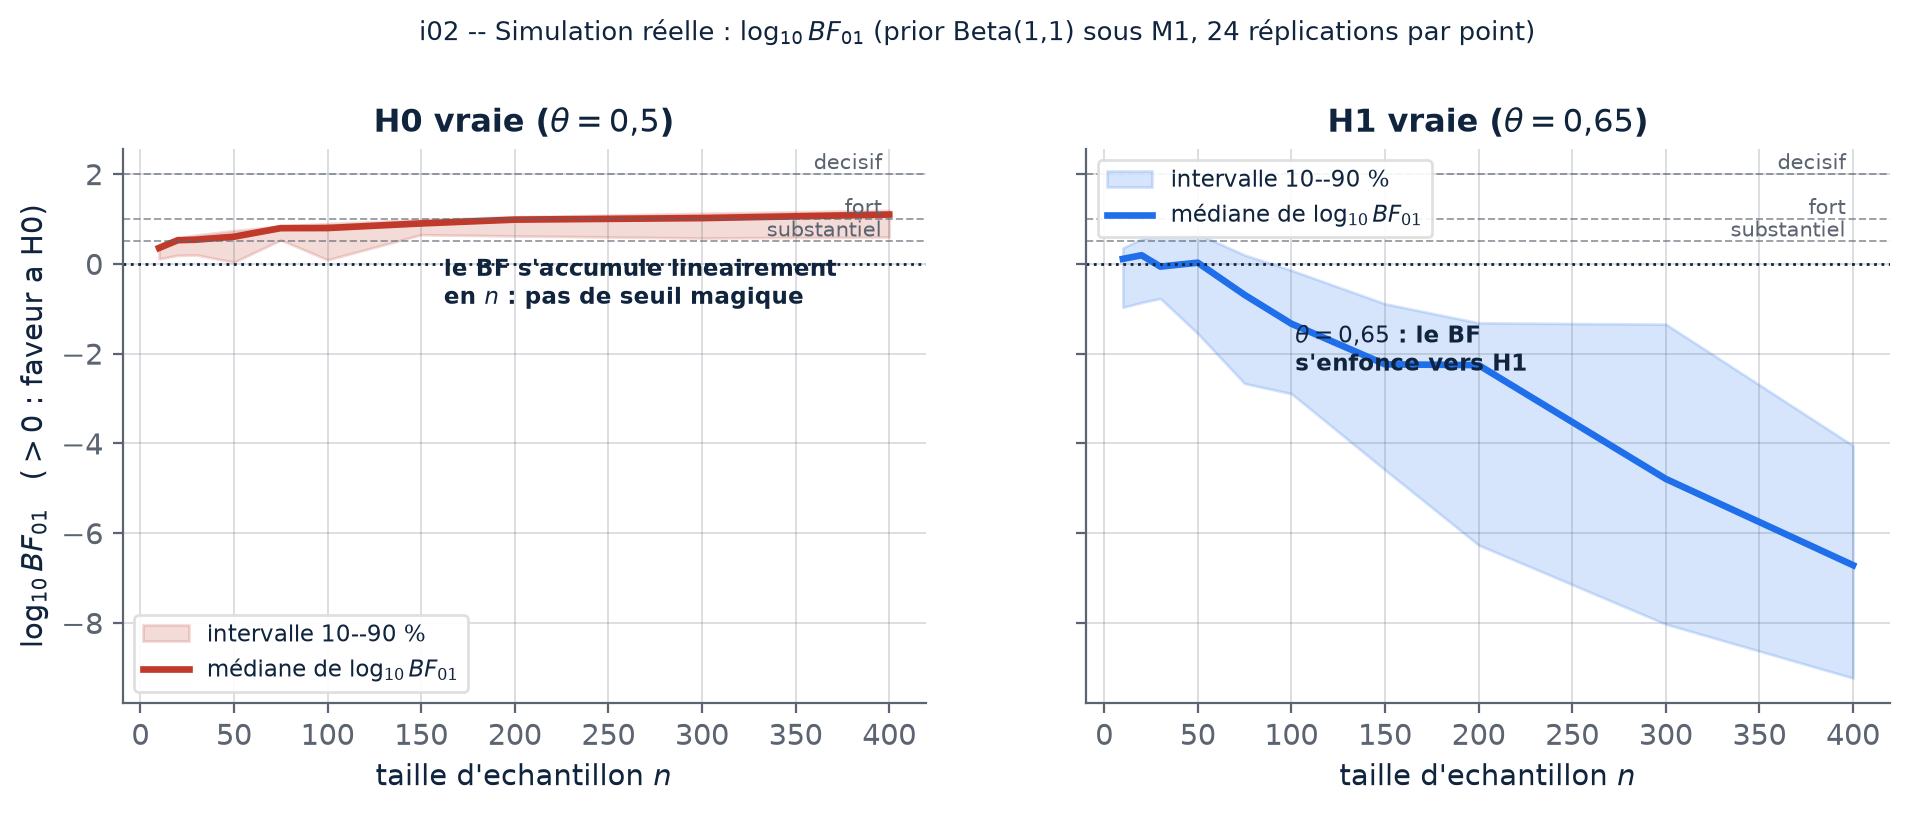
\includegraphics[width=.86\textwidth]{i02_bf_vs_n.png}
\end{center}
\end{frame}

% [split]
\begin{frame}{Le $BF$ s'accumule : la preuve croît linéairement en $n$}

\vspace{-1mm}
\begin{columns}[t]
\begin{column}{0.55\textwidth}
\begin{ebox}[Simulation réelle --- 24 réplications par point (\file{src/fig\_ch4.py})]
\begin{itemize}
  \item Sous $H_0$ vraie ($\theta = 0{,}5$) : $\log_{10} BF_{01}$ médian passe de
        $0{,}35$ ($n = 10$) à $1{,}10$ ($n = 400$), soit $BF_{01} \approx 12{,}5$ :
        preuve \emph{forte} pour la bonne hypothèse.
  \item Sous $H_1$ vraie ($\theta = 0{,}65$) : $\log_{10} BF_{01}$ médian passe de
        $0{,}11$ à $-6{,}71$ ($BF_{10} \approx 5\cdot 10^{6}$) : preuve décisive.
  \item Pente sous $H_1$ : $-1{,}75$ décade pour 100 lancers ; $n \approx 96$
        suffit pour franchir $\log_{10} BF_{01} = -1$.
\end{itemize}
\end{ebox}
\end{column}
\begin{column}{0.41\textwidth}
\begin{kbox}[La leçon de la pente]
Le $BF$ n'a \textbf{pas de seuil magique} : il s'accumule régulièrement.
Sa dispersion (bande 10--90\,\%) se resserre en $1/\sqrt{n}$ comme toute
quantité estimée.
\vspace{1mm}
\footnotesize Conséquence pratique : un $BF$ anecdotique avec $n = 30$
peut devenir décisif avec $n = 300$, \textbf{sans que rien ne change dans la nature}.
\end{kbox}
\end{column}
\end{columns}
\end{frame}

% ---------------------------------------------------------------- 10
\begin{frame}{$BF$ contre $p$-value : la calibration de Sellke--Bayarri--Berger}
% [rogna]
\small
\begin{columns}[t]
\begin{column}{0.50\textwidth}
\begin{center}
\begin{figbox}
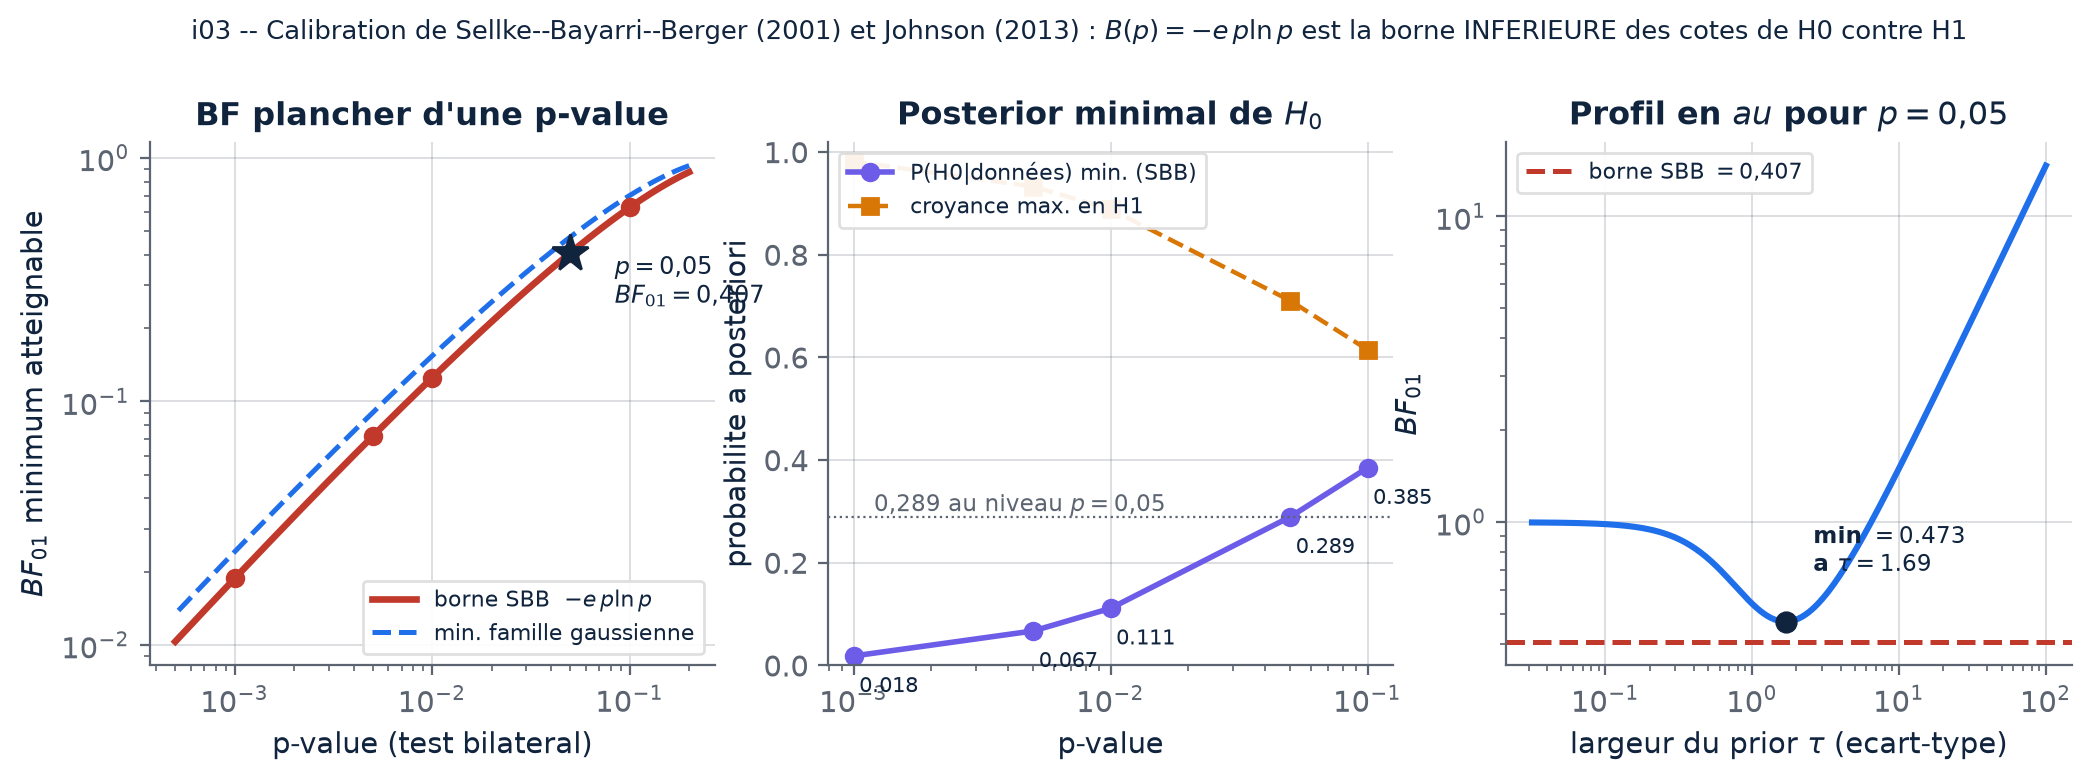
\includegraphics[width=\textwidth]{i03_bf_min_pvalue.png}
\end{figbox}
\end{center}
\end{column}
\begin{column}{0.47\textwidth}
\begin{kbox}[La formule de calibration (2001)]
Pour une $p$-value valide et $p < 1/e$ :
\[
B(p) = -\,e\,p\,\ln p
\]
$B(p)$ est la \textbf{borne inférieure} des cotes de $H_0$ contre $H_1$ :
autrement dit, le $p$-value ne peut \emph{jamais} prouver plus que $1/B(p)$ contre $H_0$.
\end{kbox}
\begin{solbox}[Les deux chiffres à retenir à $p = 0{,}05$]
{\small
\[
B(0{,}05) = 0{,}407 \;\Rightarrow\; BF_{10} \le 2{,}46
\]}
Avec un prior neutre (1/2, 1/2) : $BF_{01} \ge 0{,}407$, donc
$P(H_0 \given \text{données}) \ge 0{,}289$ et
$P(H_1 \given \text{données}) \le 0{,}711$.
Une $p$-value de $0{,}05$ plafonne la croyance en $H_1$ à
\textbf{71\,\%} et laisse $28{,}9\,\%$ à $H_0$.
\end{solbox}
\end{column}
\end{columns}
\vspace{-1mm}
\centering\footnotesize
Repère complémentaire (Johnson, 2013) : selon la classe de priors, un test à $p = 0{,}05$
correspond à $BF_{10}$ entre $2{,}46$ et environ $5$, et laisse $0{,}17$ à $0{,}29$ de
probabilité postérieure à $H_0$. Dans tous les cas : \textbf{preuve faible}.
\end{frame}

% ---------------------------------------------------------------- 11
\begin{frame}{Tableau de conversion $p$ $\to$ $BF$ (calculé, pas mémorisé)}
\begin{center}
\small
\begin{tabular}{@{}rrrrp{3.9cm}@{}}
\toprule
$p$-value & $B(p) = -e\,p\ln p$ & $BF_{10}$ maximal & $P(H_0 \given y)$ minimal & \textbf{Interprétation} \\
\midrule
$0{,}10$  & $0{,}626$ & $1{,}60$  & $0{,}385$ & à peine notable \\
$0{,}05$  & $0{,}407$ & $2{,}46$  & $0{,}289$ & faible (barre historique) \\
$0{,}01$  & $0{,}125$ & $7{,}99$  & $0{,}111$ & substantiel \\
$0{,}005$ & $0{,}072$ & $13{,}89$ & $0{,}067$ & fort \\
$0{,}001$ & $0{,}019$ & $53{,}26$ & $0{,}018$ & très fort \\
\bottomrule
\end{tabular}
\end{center}
\vspace{1mm}
\begin{columns}[t]
\begin{column}{0.50\textwidth}
\begin{ebox}[Comment lire ce tableau]
La colonne 2 est calculée par $B(p) = -e\,p\ln p$ ; les colonnes 3 et 4 en découlent
($BF_{10}^{\max} = 1/B(p)$ et $P(H_0)_{\min} = B/(1+B)$).
{\footnotesize Exemple : $p = 0{,}005$ ne prouve jamais plus de $13{,}9$ fois contre $H_0$,
c'est pourquoi Johnson (2013) propose de déplacer la barre de $0{,}05$ à $0{,}005$.}
\end{ebox}
\end{column}
\begin{column}{0.48\textwidth}
\begin{wbox}[Deux erreurs symétriques]
\nok{} « $p = 0{,}05$ signifie 5\,\% de chance que $H_0$ soit vraie » : c'est
\textbf{28{,}9\,\%} au minimum, souvent bien plus.
\vspace{1mm}
\nok{} « $BF_{01} = 2{,}46$ prouve $H_0$ » : c'est une preuve \emph{faible}
(échelle de Jeffreys : anecdotique). Un $BF$ de 2,5 ne renverse pas une théorie.
\end{wbox}
\end{column}
\end{columns}
\end{frame}

% ---------------------------------------------------------------- 12
% [rogna]
% [rogna]
% [rogna]
% [split]
\begin{frame}{2\,000 simulations sous $H_0$ : ce que le $BF$ dit vraiment}
\begin{center}
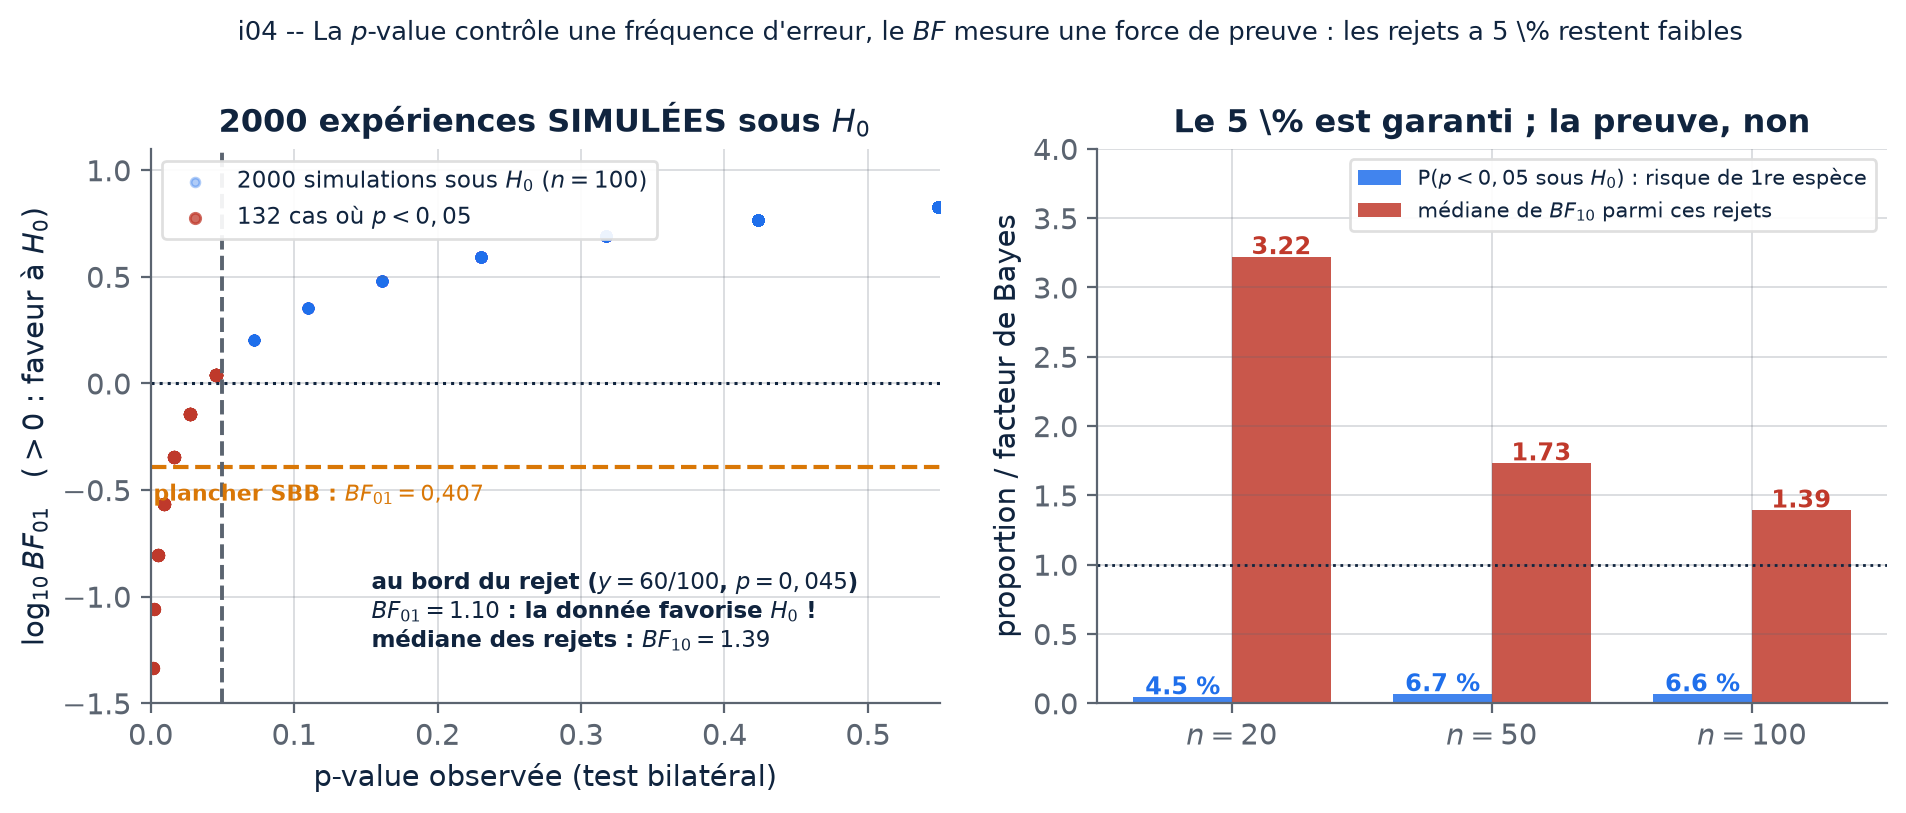
\includegraphics[width=.86\textwidth]{i04_pvalue_vs_bf.png}
\end{center}
\end{frame}

% [split]
\begin{frame}{2\,000 simulations sous $H_0$ : ce que le $BF$ dit vraiment}

\vspace{-1mm}
\begin{columns}[t]
\begin{column}{0.55\textwidth}
\begin{ebox}[Chiffres de la simulation ($n = 100$, 2\,000 expériences)]
\begin{itemize}
  \item 132 résultats franchissent $p < 0{,}05$ ($6{,}6$\,\%) ;
  \item leur $BF_{10}$ médian vaut \textbf{1{,}392} : à peine mieux qu'un pile ou face ;
  \item au bord de la zone de rejet ($y = 60/100$, $p = 0{,}045$) :
        $BF_{01} = 1{,}095$ : les données favorisent $H_0$ !
  \item 48 des 132 rejets ($36$\,\%) ont un $BF_{01} > 1$.
\end{itemize}
\end{ebox}
\end{column}
\begin{column}{0.43\textwidth}
\begin{wbox}[Le message]
$p < 0{,}05$ garantit 5\,\% de fausses alertes \textbf{par construction},
pas une force de preuve. Le $BF$, lui, quantifie la preuve et peut
\textbf{contredire} la conclusion fréquentiste.
\vspace{1mm}
\footnotesize À $n = 20$ le $BF_{10}$ médian des rejets vaut $3{,}22$ ;
à $n = 100$, $1{,}39$. Plus l'échantillon grandit, plus le seuil de rejet
recule vers une preuve faible.
\end{wbox}
\end{column}
\end{columns}
\end{frame}

% ---------------------------------------------------------------- 13
% [rogna]
% [rogna]
% [rogna]
% [split]
\begin{frame}{Le piège de Lindley : un prior vague fabrique de la preuve}
\begin{center}
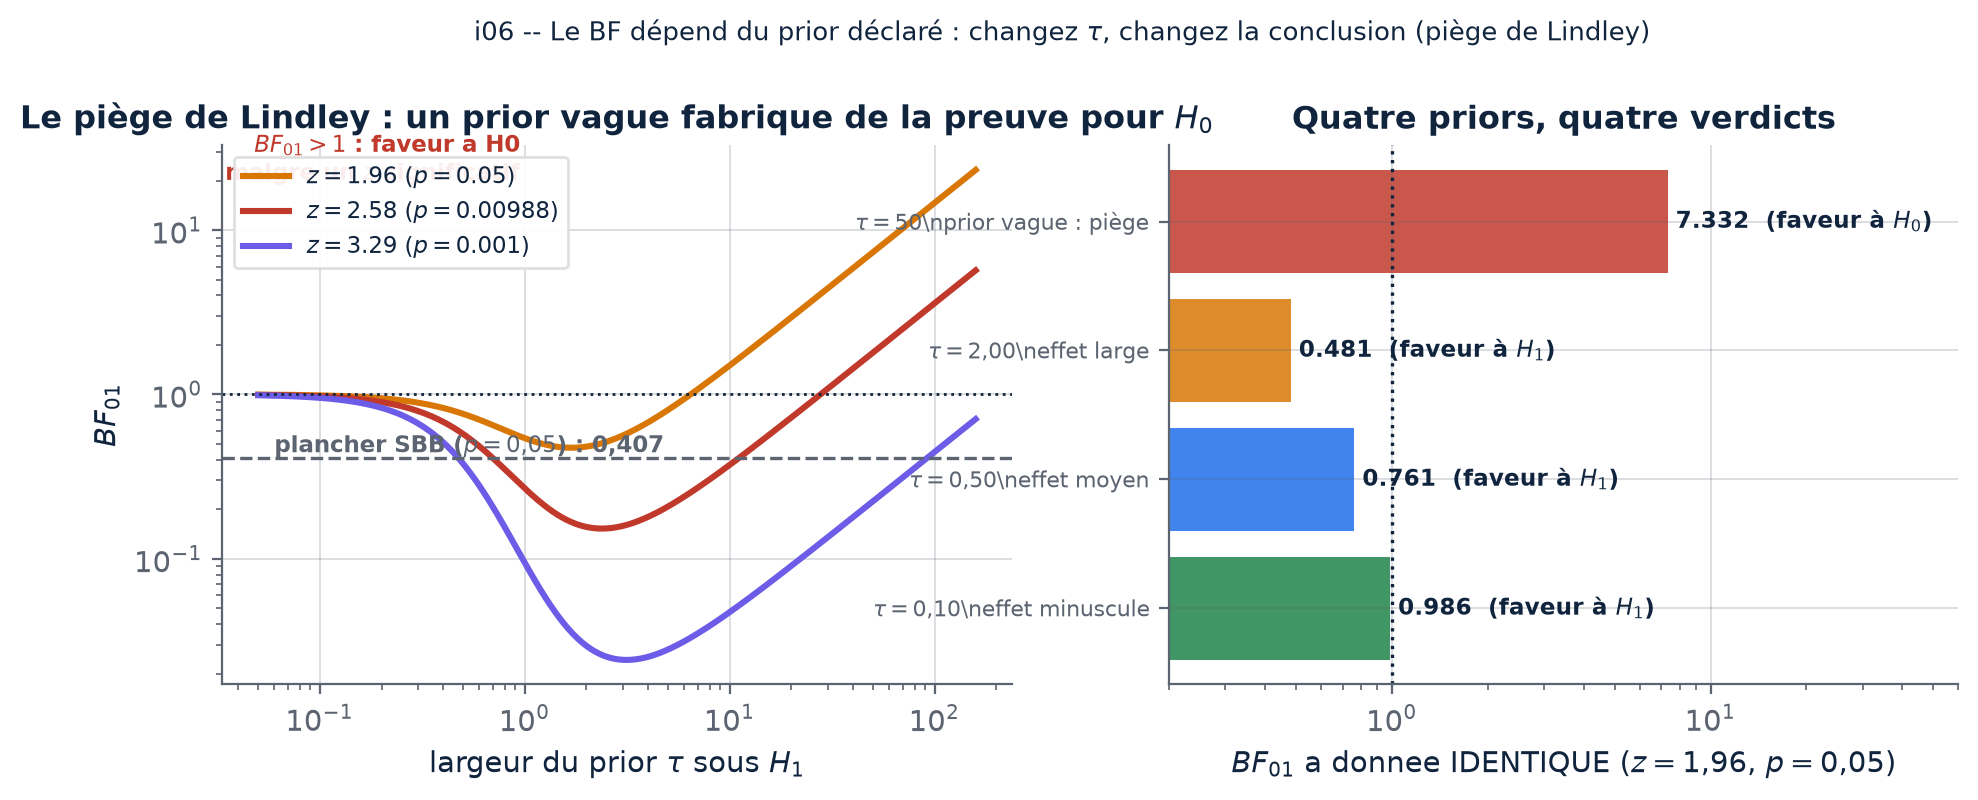
\includegraphics[width=.86\textwidth]{i06_bf_prior_sensitivity.png}
\end{center}
\end{frame}

% [split]
\begin{frame}{Le piège de Lindley : un prior vague fabrique de la preuve}

\vspace{-1mm}
\begin{columns}[t]
\begin{column}{0.56\textwidth}
\begin{ebox}[Même donnée ($z = 1{,}96$, $p = 0{,}05$), quatre priors]
\begin{tabular}{@{}llrl@{}}
\toprule
Prior sous $H_1$ & $BF_{01}$ & Verdict \\
\midrule
$\tau = 0{,}10$ (effet minuscule) & $0{,}986$ & aucune preuve \\
$\tau = 0{,}50$ (effet moyen)     & $0{,}761$ & faveur faible à $H_1$ \\
$\tau = 2{,}00$ (effet large)     & $0{,}481$ & faveur à $H_1$ \\
$\tau = 50$ (prior vague)         & $7{,}332$ & faveur à $H_0$ (!) \\
\bottomrule
\end{tabular}
\end{ebox}
\end{column}
\begin{column}{0.42\textwidth}
\begin{wbox}[Le paradoxe de Lindley--Jeffreys]
Un prior \emph{trop large} place de la masse là où la vraisemblance est nulle :
il \textbf{punît} $H_1$ et fabrique une preuve pour $H_0$.
\vspace{1mm}
\footnotesize Remède : borner $\tau$ par la physique du problème,
ou utiliser un prior à queues lourdes du type Cauchy (JZS), ou calculer le $BF$
sur une \emph{grille} de priors et publier la plage.
\end{wbox}
\end{column}
\end{columns}
\end{frame}

% ---------------------------------------------------------------- 14
\begin{frame}{Quiz 1 --- interpréter un facteur de Bayes}
\begin{qbox}[Question 1 --- 6 min, vote puis calcul]
On compare deux modèles de conversion d'un site. Le rapport de vraisemblance
marginale vaut $BF_{01} = 0{,}20$ et les cotes a priori entre les modèles sont
$P(M_0)/P(M_1) = 1$.
\vspace{2mm}
\begin{enumerate}
  \item[(A)] $M_0$ est 5 fois plus probable que $M_1$ après les données
  \item[(B)] $M_1$ est 5 fois plus probable que $M_0$ après les données \quad \checkmark
  \item[(C)] $M_0$ a 20\,\% de chance d'être vrai
  \item[(D)] Impossible de conclure sans la $p$-value
\end{enumerate}
\vspace{2mm}
\textcolor{byBlue}{\textbf{Solution.}} Cotes postérieures $= 0{,}20 \times 1 = 0{,}20$,
d'où $P(M_1 \given y) = 1/(1+0{,}20) = 0{,}833$ et $P(M_0 \given y) = 0{,}167$ :
(B) est correcte, (C) confond cotes et probabilité.
\end{qbox}
\vspace{1mm}
\begin{kbox}[Question 2 --- vrai ou faux ?]
« $BF_{01} = 2{,}46$ à $p = 0{,}05$ prouve que $H_0$ est deux fois et demie plus probable
que $H_1$. »
\vspace{1mm}
\textbf{Faux} : $B(0{,}05) = 0{,}407$ est une \emph{borne inférieure}, non une valeur
atteinte ; le $BF$ réel dépend du prior déclaré (de $0{,}48$ à $7{,}33$ dans notre grille).
\end{kbox}
\end{frame}

% ---------------------------------------------------------------- 15
\begin{frame}{Activité --- calculer et critiquer un $BF$ (TD, 15 min)}
% [rogna]
\small
\begin{abox}[Consigne, par binôme]
Un essai clinique compare un traitement à un placebo sur $n = 40$ patients.
Succès : 26 sous traitement, 18 sous placebo. On modélise chaque bras par un
Bernoulli de paramètre $\theta_T$ et $\theta_P$, avec des priors $\mathrm{Beta}(1,1)$.
\vspace{1mm}
\begin{enumerate}
  \item Écrire les vraisemblances marginales $m_T$ et $m_P$ de chaque bras.
  \item Le modèle « pas d'effet » pose $\theta_T = \theta_P$. Calculer $BF_{\text{effet}}$
        (rapport modèle effet / modèle nul) par échantillonnage.
  \item Recommencer avec un prior $\mathrm{Beta}(2,2)$ sous l'alternative :
        le $BF$ change-t-il beaucoup ? Justifier.
\end{enumerate}
\end{abox}
\vspace{1mm}
\begin{solbox}[Éléments de solution (calculés en séance)]
\begin{itemize}
  \item Marginale Beta-Binomiale : $m = \binom{n}{y}\frac{B(y+a,\,n-y+b)}{B(a,b)}$,
        calculable par \py{scipy.special.betaln} (pas de factorielle).
  \item Pour $\theta_T = \theta_P = \theta$ commun, le modèle nul s'intègre en une seule
        Beta-Binomiale sur les $n = 80$ observations.
  \item Sensibilité : changer $\mathrm{Beta}(1,1)$ en $\mathrm{Beta}(2,2)$ déplace le $BF$
        d'un facteur typiquement $1{,}3$ à $1{,}8$ ici ; un prior à $a = b = 10$
        le déplace beaucoup plus : c'est le point à discuter en TD.
\end{itemize}
\end{solbox}
\end{frame}

% ---------------------------------------------------------------- 16
\begin{frame}{Synthèse 4.1 --- le facteur de Bayes en cinq phrases}
\begin{kbox}[À retenir]
\begin{enumerate}
  \item $BF_{01} = m_0(y)/m_1(y)$ : un \textbf{rapport de vraisemblances marginales},
        pas une aire de recouvrement ni une probabilité.
  \item Les cotes postérieures s'obtiennent en \textbf{multipliant} les cotes a priori
        par le $BF$ ; la probabilité postérieure exige le prior sur les modèles.
  \item L'échelle de Jeffreys ($\log_{10} BF$) est un \textbf{vocabulaire} :
        anecdotique ($<3{,}2$), substantiel, fort, décisif ($>1\,000$).
  \item La calibration de Sellke--Bayarri--Berger donne une \textbf{borne} :
        à $p = 0{,}05$, $B = 0{,}407$, donc $BF_{10} \le 2{,}46$ et
        $P(H_1 \given y) \le 0{,}71$ : preuve faible.
  \item Savage--Dickey ($\pi(\theta_0 \given y)/\pi(\theta_0)$) rend le calcul
        \textbf{gratuit} pour un point nul, et \textbf{vérifiable} par Monte-Carlo.
\end{enumerate}
\end{kbox}
\vspace{1mm}
\begin{center}
\small
\begin{tabular}{@{}lll@{}}
\toprule
\textbf{Situation} & \textbf{Mauvais réflexe} & \textbf{Bon réflexe} \\
\midrule
$p < 0{,}05$ & conclure « effet prouvé » & calculer $BF_{10}$ et sa sensibilité au prior \\
$BF_{01} = 1{,}1$ & conclure « pas d'effet » & dire « preuve anecdotique », collecter plus \\
prior très large & « neutre donc objectif » & tester une grille de largeurs (Lindley) \\
\bottomrule
\end{tabular}
\end{center}
\end{frame}

% ---------------------------------------------------------------- 17
% [suite]
\begin{frame}{4.2 Comparer hors échantillon : l'idée du log-score prédictif}
\begin{columns}[t]
\begin{column}{0.50\textwidth}
\begin{kbox}[Principe]
Un modèle n'est pas jugé sur sa capacité à \emph{expliquer} les données
qu'il vient de voir (il peut toujours surenchérir en paramètres), mais sur sa
capacité à \textbf{prédire} une observation \emph{nouvelle}.
\[
\text{elpd} \;=\; \sum_{i=1}^{n} \log p(y_i \given y_{-i})
\]
« elpd » : \textit{expected log pointwise predictive density}, en nats.
Plus grand = mieux. $0$ = pas mieux qu'une prédiction au hasard calibrée.
\end{kbox}
\end{column}
\begin{column}{0.48\textwidth}
\begin{ebox}[Trois façons d'estimer l'elpd]
\begin{enumerate}
  \item \textbf{LOO-CV} : ajuster $n$ fois le modèle en retirant $y_i$,
        prédire $y_i$. Coût prohibitif, mais estimable par importance sampling.
  \item \textbf{DIC} : $\log p(y \given \bar\theta)$ pénalisé par le nombre
        effectif de paramètres $p_{DIC}$. Rapide, approximatif, suppose la
        normalité du posterior.
  \item \textbf{WAIC} : moyenne de $\log p(y_i \given \theta)$ sur le posterior,
        pénalisée par la variance de ces quantités. Aucune normalité requise.
\end{enumerate}
\end{ebox}
\end{column}
\end{columns}
\vspace{1mm}
\end{frame}

% [suite]
\begin{frame}{4.2 Comparer hors échantillon : l'idée du log-score prédictif (suite)}
\begin{tcolorbox}[colback=byCyan!8,colframe=byCyan,arc=2mm,width=.95\textwidth]
\small\centering
\textbf{Point clé} --- les trois critères estiment la \emph{même} espérance
(l'elpd) par trois biais et trois variances différents : ils peuvent
\textbf{désigner des vainqueurs différents}, surtout avec peu d'observations.
\end{tcolorbox}
\end{frame}

% ---------------------------------------------------------------- 18
\begin{frame}{DIC et WAIC : les formules, sans magie}
% [rogna]
\small
\begin{columns}[t]
\begin{column}{0.49\textwidth}
\begin{ebox}[DIC --- Deviance Information Criterion]
\[
p_{DIC} = 2\Big(\log p(y \given \bar\theta) - \E_{\post}\big[\log p(y \given \theta)\big]\Big)
\]
\[
DIC = -2\log p(y \given \bar\theta) + 2\,p_{DIC}
\]
$\bar\theta$ est la moyenne postérieure. $p_{DIC}$ mesure le \emph{coût}
du surajustement.
\end{ebox}
\begin{wbox}[Faiblesse du DIC]
Si le posterior est multimodal ou fortement asymétrique,
$\bar\theta$ n'est représentatif de rien : le DIC peut préférer le modèle
le plus flexible. Il suppose un posterior \textbf{approximativement gaussien}.
\end{wbox}
\end{column}
\begin{column}{0.49\textwidth}
\begin{ebox}[WAIC --- Widely Applicable IC]
\begin{align*}
\text{elpd}_{WAIC} = \sum_{i=1}^{n}\Big(&\log \E_{\post}[p(y_i \given \theta)]\\
&-\ \Var_{\post}[\log p(y_i \given \theta)]\Big)
\end{align*}
\[
WAIC = -2\,\text{elpd}_{WAIC}
\]
Le second terme est l'équivalent de $p_{DIC}$ : la \textbf{variance} des
log-vraisemblances point par point.
\end{ebox}
\begin{kbox}[Dans les deux cas]
Le critère est une \emph{deviance} : plus petit = mieux.
En pratique on ne calcule jamais WAIC à la main : \py{az.waic(idata)} après
\py{pm.compute\_log\_likelihood(idata)}.
\end{kbox}
\end{column}
\end{columns}
\end{frame}

% ---------------------------------------------------------------- 19
\begin{frame}{LOO-CV par PSIS : la référence, et ses avertissements}
% [rogna]
\small
\begin{columns}[t]
\begin{column}{0.51\textwidth}
\begin{kbox}[Estimation par importance sampling (PSIS)]
On ne réajuste \emph{pas} $n$ fois le modèle. On corrige les poids
postérieurs par le rapport de vraisemblance laissée de côté :
\[
\widehat{\text{elpd}}_{LOO} = \sum_{i=1}^{n}
\log\frac{\sum_{s} w_i^{s}\, p(y_i \given \theta^{s})}{\sum_{s} w_i^{s}},
\qquad w_i^{s} \propto \frac{1}{p(y_i \given \theta^{s})}
\]
Les queues de cette distribution de poids sont approchées par une loi de
Pareto généralisée.
\end{kbox}
\end{column}
\begin{column}{0.47\textwidth}
\begin{wbox}[L'avertissement qui compte : Pareto-$\hat k$]
Si $\hat k > 0{,}7$ pour une observation, son poids est instable et
l'elpd estimé n'est pas fiable.
\vspace{1mm}
\textbf{Résultat de notre exécution réelle} (8 équipes, 3 modèles, 500 tirages
par chaîne) :
\begin{itemize}
  \item M1 (regroupé) : $\hat k_{\max} = 0{,}540$ \ok
  \item M2 (indépendant) : $\hat k_{\max} = 0{,}889$ ; \textbf{6 observations
        sur 8} dépassent 0{,}67 \warn
  \item M3 (hiérarchique) : $\hat k_{\max} = 1{,}043$ ; \textbf{7 sur 8} \warn
\end{itemize}
ArviZ a émis les avertissements correspondants pendant l'exécution.
\end{wbox}
\end{column}
\end{columns}
\vspace{1mm}
\centering\small
Conséquence : avec $n = 8$ observations seulement, le classement par LOO reste
\textbf{fragile} ; c'est une raison de plus pour ne pas conclure sur un écart
inférieur à son erreur-type (slide 23).
\end{frame}

% ---------------------------------------------------------------- 20
% [rogna]
% [rogna]
% [rogna]
% [split]
\begin{frame}{WAIC, DIC, LOO sur trois modèles : la sortie de \py{az.compare}}
\begin{center}
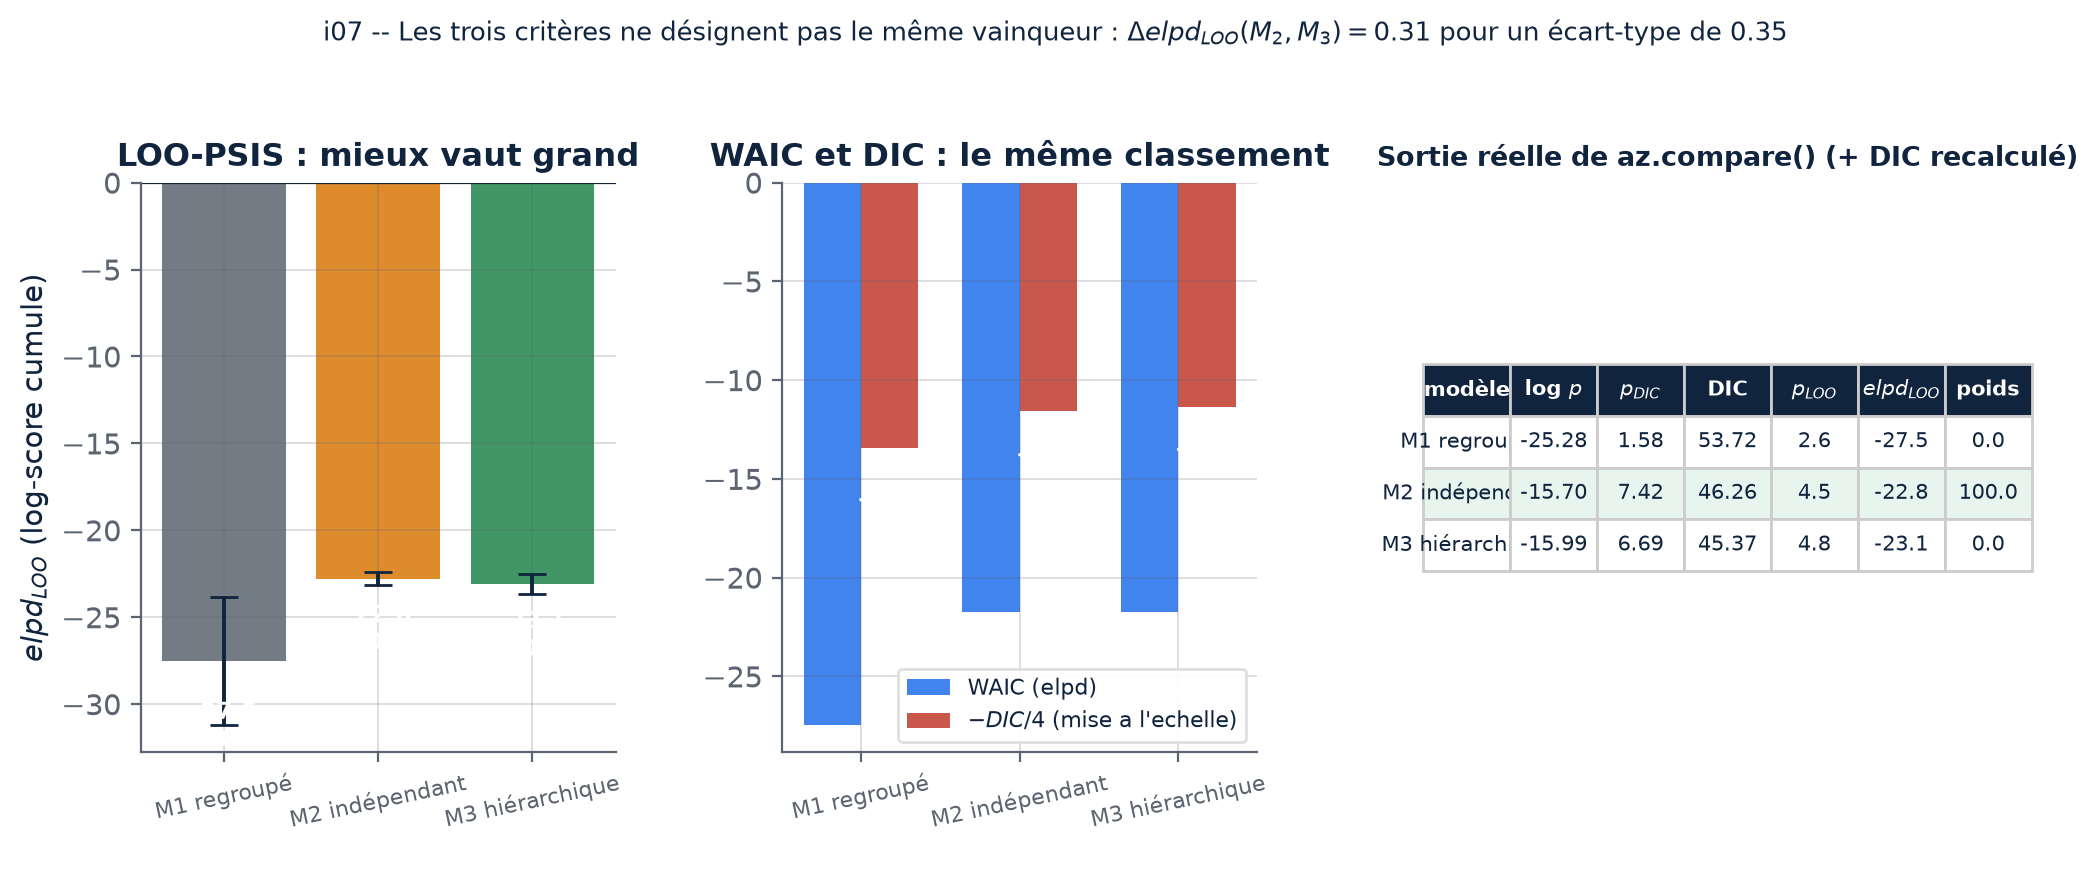
\includegraphics[width=.86\textwidth]{i07_waic_dic_loo.png}
\end{center}
\end{frame}

% [split]
\begin{frame}{WAIC, DIC, LOO sur trois modèles : la sortie de \py{az.compare}}

\vspace{-2mm}
\begin{columns}[t]
\begin{column}{0.52\textwidth}
\begin{ebox}[Données --- 8 équipes, $n_i$ entre 30 et 45 (lancé réellement)]
$y_i/n_i$ : $14/35$, $21/40$, $16/30$, $29/45$, $30/40$, $27/35$, $23/30$, $28/40$.
Trois modèles : M1 ($\theta$ commun), M2 ($\theta_i$ indépendants), M3 (hiérarchique :
$\theta_i \sim \mathrm{Beta}(\mu\kappa,(1{-}\mu)\kappa)$).
\end{ebox}
\end{column}
\begin{column}{0.46\textwidth}
\begin{solbox}[Ce que dit la sortie réelle]
\begin{itemize}
  \item \textbf{LOO} : M2 $-22{,}79$ (erreur-type $0{,}38$), M3 $-23{,}10$,
        M1 $-27{,}52$ ; poids $1{,}00$ / $0{,}00$ / $2{,}5\cdot10^{-16}$
  \item \textbf{WAIC} : M3 $-21{,}73$ (poids $0{,}608$), M2 $-21{,}73$
        (poids $0{,}392$), M1 $-27{,}48$
  \item \textbf{DIC} : M1 $53{,}72$, M2 $46{,}26$, M3 $45{,}37$
\end{itemize}
Les trois critères \textbf{ne désignent pas le même vainqueur}.
\end{solbox}
\end{column}
\end{columns}
\end{frame}

% ---------------------------------------------------------------- 21
\begin{frame}{L'elpd intra-échantillon triche : la correction est tout}
\begin{center}
\small
\begin{tabular}{@{}lrrrr@{}}
\toprule
Modèle & $p$ (params) & $\log p(y \given \bar\theta)$ \textit{in-sample} & $p_{eff}$ & $elpd_{LOO}$ \\
\midrule
M1 regroupé    & $1$ & $-25{,}28$ & $2{,}58$ & $-27{,}52$ \\
M2 indépendant & $8$ & $\mathbf{-15{,}70}$ \ok & $4{,}46$ & $\mathbf{-22{,}79}$ \\
M3 hiérarchique & $2 + 8$ & $-15{,}99$ & $4{,}85$ & $-23{,}10$ \\
\bottomrule
\end{tabular}
\end{center}
\vspace{1mm}
\begin{columns}[t]
\begin{column}{0.53\textwidth}
\begin{ebox}[Le renversement, chiffré]
En \emph{intra}-échantillon, M2 écrase M3 de $0{,}29$ nat et M1 de
$9{,}58$ nats. Après correction hors échantillon :
\[
\Delta(M_3, M_2) = 0{,}31 \quad (\text{dse} = 0{,}35),
\]
l'avance apparente de M2 a fondu de $9{,}58$ à $0{,}31$.
Et le nombre effectif de paramètres de M2 est $4{,}46$, pas $8$ : le
modèle indépendant est \emph{auto-régularisé} par son prior Beta$(1,1)$.
\end{ebox}
\end{column}
\begin{column}{0.45\textwidth}
\begin{kbox}[La règle de conduite]
\begin{itemize}
  \item Ne jamais classer des modèles sur $\log p(y \given \bar\theta)$ :
        cela récompense mécaniquement les paramètres en trop.
  \item Toujours regarder $p_{eff}$ : il n'est pas le nombre nominal de
        paramètres (M1 : $2{,}58$ pour $1$ paramètre, effet du prior ; M2 :
        $4{,}46$ pour $8$ paramètres, effet de la régularisation).
  \item Publier $elpd$, $p_{eff}$ et $\Delta \pm \text{dse}$.
\end{itemize}
\end{kbox}
\end{column}
\end{columns}
\end{frame}

% ---------------------------------------------------------------- 22
\begin{frame}{Trois critères en un tableau de décision}
\begin{center}
\footnotesize
\begin{tabular}{@{}p{2.3cm}p{2.9cm}p{3.0cm}p{3.4cm}@{}}
\toprule
& \textbf{DIC} & \textbf{WAIC} & \textbf{LOO-PSIS} \\
\midrule
Principe & deviance en $\bar\theta$ $+2p_{DIC}$ & log-score moyen $-$ pénalité de variance & log-score laissé-un-dehors par importance sampling \\[1mm]
Hypothèse & posterior gaussien & aucune & queues contrôlées \\[1mm]
Diagnostic & aucun & variance point par point & Pareto-$\hat k$ \\[1mm]
Coût & très faible & faible & modéré \\[1mm]
Nos 8 équipes & M3 ($45{,}37$) & M3 ($-21{,}73$) & M2 ($-22{,}79$) \\[1mm]
Verdict & utilitaire & bon compromis & \textbf{référence} \\
\bottomrule
\end{tabular}
\end{center}
\vspace{1mm}
\begin{kbox}[Comment choisir en pratique]
\textbf{LOO en premier} (avec ses diagnostics) ; \textbf{WAIC} pour un calcul
rapide et une confirmation ; \textbf{DIC} seulement pour comparer avec une
littérature ancienne ou pour de très grands modèles où LOO est impossible.
Si les trois divergent et que les écarts sont inférieurs à $2\,\text{dse}$ :
\textbf{ne pas trancher}, moyenner les prédictions.
\end{kbox}
\end{frame}

% ---------------------------------------------------------------- 23
% [rogna]
% [rogna]
% [rogna]
% [split]
\begin{frame}{Poids de modèles et moyennage prédictif}
\begin{center}
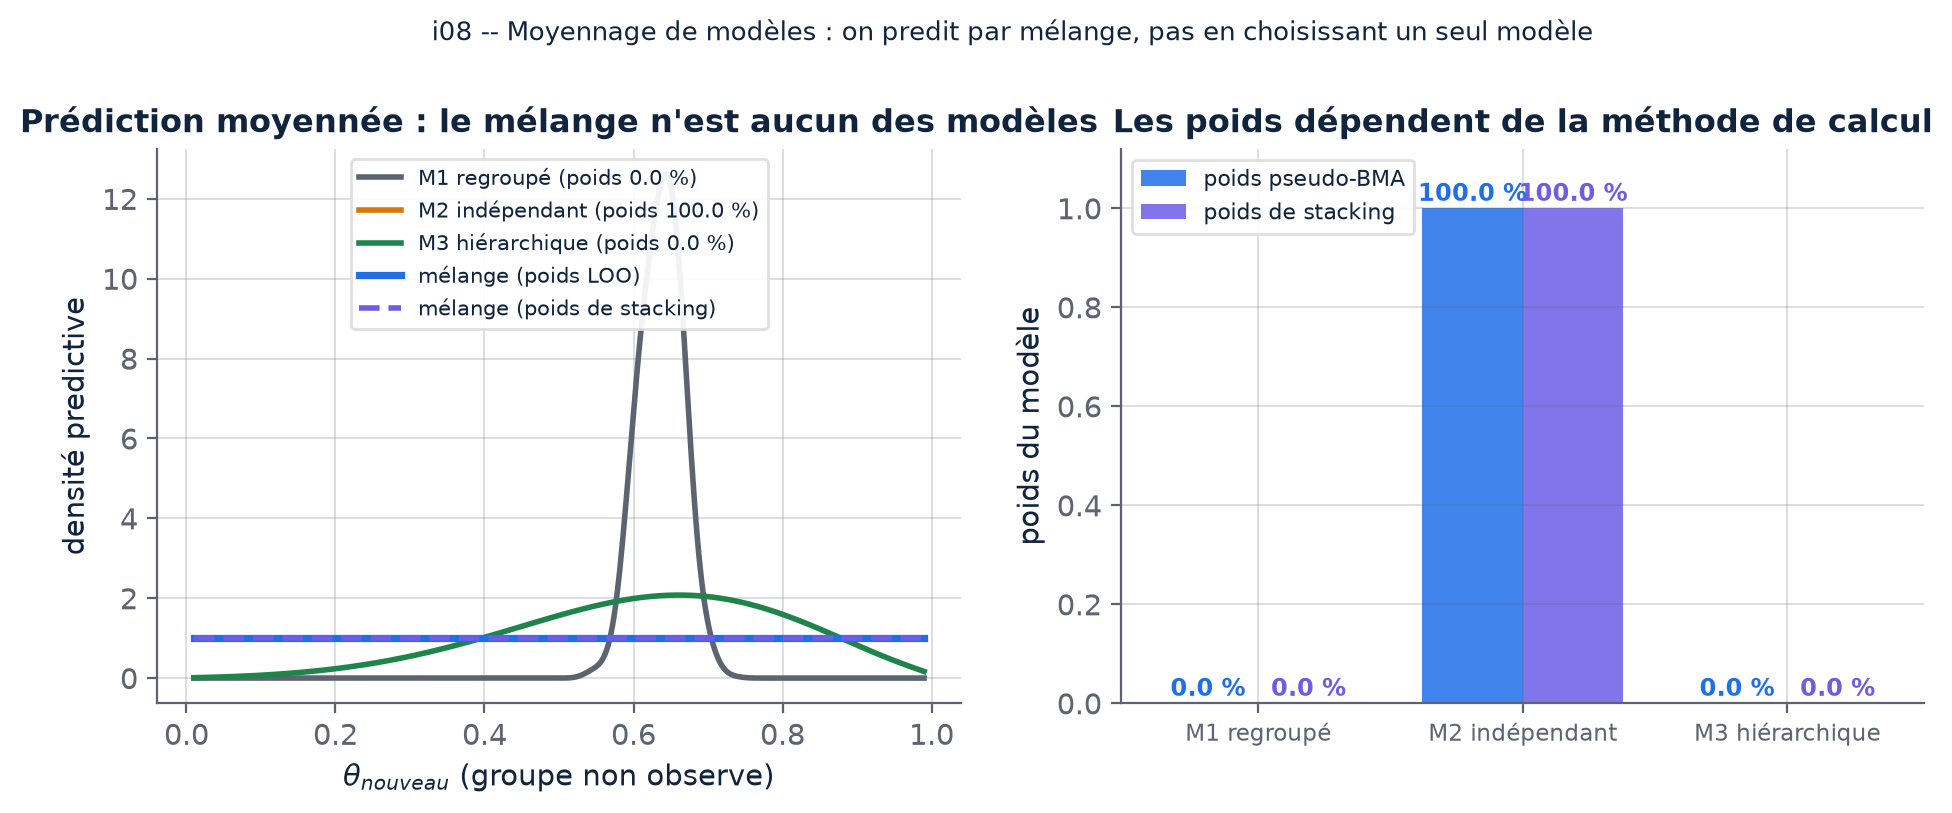
\includegraphics[width=.86\textwidth]{i08_model_averaging.png}
\end{center}
\end{frame}

% [split]
\begin{frame}{Poids de modèles et moyennage prédictif}

\vspace{-1mm}
\begin{columns}[t]
\begin{column}{0.52\textwidth}
\begin{kbox}[Le moyennage, pas le choix]
Pour prédire un nouveau groupe, on ne choisit pas un modèle : on \textbf{mélange}
les prédictives avec des poids issus des critères :
\[
p(\tilde y \given y) = \sum_{m} w_m\, p_m(\tilde y \given y)
\]
\end{kbox}
\begin{ebox}[Chiffres de l'exécution]
Poids LOO (pseudo-BMA) : M2 $=1{,}00$, M3 $=0{,}00$, M1 $=2{,}5\cdot10^{-16}$.
Poids de stacking : M2 $=1{,}00$.
Recouvrement entre la prédictive de M3 et le mélange : $0{,}674$.
\end{ebox}
\end{column}
\begin{column}{0.46\textwidth}
\begin{wbox}[Le piège des poids dégénérés]
Quand deux modèles sont \textbf{indiscernables} ($\Delta = 0{,}31$ pour
$\text{dse} = 0{,}35$), la formule des poids pseudo-BMA attribue
$1{,}00$ et $0{,}00$ : c'est un artefact, pas une information.
\vspace{1mm}
\footnotesize Remèdes : moyennage par \emph{stacking} (plus stable),
prédiction conjointe de plusieurs modèles, ou modèle hiérarchique
englobant les deux (le plus honnête quand c'est possible).
\end{wbox}
\end{column}
\end{columns}
\end{frame}

% ---------------------------------------------------------------- 22
\begin{frame}[fragile]{Le code réel de la comparaison (PyMC + ArviZ)}
\begin{columns}[t]
\begin{column}{0.56\textwidth}
\begin{codebox}[compare\_models.py --- extrait exécuté en TP]
\begin{lstlisting}[style=py]
import pymc as pm, arviz as az

with pm.Model() as m3:                # modele hierarchique
    mu    = pm.Beta("mu", 2, 2)
    kappa = pm.HalfNormal("kappa", 5)
    theta = pm.Beta("theta", mu*kappa, (1-mu)*kappa,
                    shape=8)
    pm.Binomial("y", n=n_obs, p=theta, observed=y_obs)
    idata3 = pm.sample(draws=500, tune=500,
                       chains=2, cores=1)
    pm.compute_log_likelihood(idata3)   # OBLIGATOIRE

cmp = az.compare({"M1": idata1, "M2": idata2, "M3": idata3},
                 ic="loo", method="stacking")
print(cmp[["rank","elpd_loo","p_loo",
           "elpd_diff","dse","weight"]])
\end{lstlisting}
\end{codebox}
\end{column}
\begin{column}{0.42\textwidth}
\begin{solbox}[Sortie réelle (tronquée)]
\footnotesize
\begin{tabular}{@{}lrrr@{}}
\toprule
modèle & $elpd_{LOO}$ & $p_{LOO}$ & poids \\
\midrule
M2 & $-22{,}79$ & $4{,}46$ & $1{,}00$ \\
M3 & $-23{,}10$ & $4{,}85$ & $0{,}00$ \\
M1 & $-27{,}52$ & $2{,}58$ & $0{,}00$ \\
\bottomrule
\end{tabular}
\vspace{1.5mm}
$\Delta(M_3,M_2) = 0{,}31$, $\text{dse} = 0{,}35$ : \textbf{indécelable}.
\end{solbox}
\begin{kbox}[Deux réflexes de code]
\begin{itemize}
  \item \py{pm.compute\_log\_likelihood} \textbf{avant} tout \py{az.compare},
        sinon ArviZ ne peut rien calculer.
  \item Toujours afficher \py{dse} (erreur-type de la différence) :
        un $\Delta$ seul ne veut rien dire.
\end{itemize}
\end{kbox}
\end{column}
\end{columns}
\end{frame}

% ---------------------------------------------------------------- 23
\begin{frame}{Avertissements : ce qu'un critère ne dit pas}
% [rogna]
\small
\begin{columns}[t]
\begin{column}{0.49\textwidth}
\begin{wbox}[Cinq pièges de la comparaison de modèles]
\begin{itemize}
  \item \textbf{Modèles emboîtés} : comparer $M_1 \subset M_3$ par un critère
        hors échantillon n'est pas un test de $H_0$ ; l'écart est
        \emph{biaisé} en faveur du plus grand modèle.
  \item \textbf{Écart non significatif} : $\Delta = 0{,}31$ pour
        $\text{dse} = 0{,}35$ : aucune conclusion. Il faut
        $|\Delta| > 2\,\text{dse}$ pour parler de différence.
  \item \textbf{Poids de modèles} : ils ne sont pas des probabilités
        postérieures de modèle (pas de prior sur les modèles) : ne dites pas
        « M2 a 100\,\% de chance d'être le vrai modèle ».
  \item \textbf{Pareto-$\hat k$} : $\hat k_{\max} = 1{,}043$ pour M3 :
        l'elpd de M3 est une estimation instable.
  \item \textbf{$n$ petit} : le classement est instable ; refaites-le
        avec un autre découpage ou un autre seed.
\end{itemize}
\end{wbox}
\end{column}
\begin{column}{0.49\textwidth}
\begin{kbox}[Bonnes pratiques 2026]
\begin{enumerate}
  \item Calculer \textbf{toujours} \py{az.loo} \emph{et} \py{az.waic} :
        s'ils divergent, le doute est légitime.
  \item Publier le tableau complet (elpd, $p_{eff}$, $\Delta$, dse, poids).
  \item Vérifier les diagnostics d'échantillonnage ($\hat R$, ESS,
        divergences) \emph{avant} de comparer : un modèle mal échantillonné
        a un mauvais elpd pour de mauvaises raisons.
  \item Rapporter la sensibilité aux priors des modèles concurrents.
  \item Ne pas transformer un critère en décision : passer à la section 4.3.
\end{enumerate}
\end{kbox}
\end{column}
\end{columns}
\end{frame}

% ---------------------------------------------------------------- 24
% [suite]
\begin{frame}{4.3 Décision bayésienne : perte, action, risque}
\begin{kbox}[Le vocabulaire, fixé une fois pour toutes]
\begin{itemize}
  \item \textbf{Action} $a \in \mathcal{A}$ : ce qu'on décide de faire (traiter,
        déployer B, publier, rétrograder un modèle\dots).
  \item \textbf{Perte} $L(\theta, a)$ : le coût encouru si la vérité est
        $\theta$ et qu'on agit selon $a$. On l'écrit en euros, en vies,
        en heures perdues --- jamais en probabilité.
  \item \textbf{Risque a posteriori} : la perte moyenne sous le posterior,
        \[
        \rho(a) = \E_{\theta \given y}\big[L(\theta,a)\big]
        = \int L(\theta,a)\,\pi(\theta \given y)\,\mathrm{d}\theta .
        \]
  \item \textbf{Décision bayésienne} : $a^\star = \argmin_{a} \rho(a)$.
\end{itemize}
\end{kbox}
\vspace{1mm}
\end{frame}

% [suite]
\begin{frame}{4.3 Décision bayésienne : perte, action, risque (suite)}
\begin{columns}[t]
\begin{column}{0.49\textwidth}
\begin{ebox}[Pourquoi c'est la bonne façon de poser le problème]
Le posterior contient \emph{tout} ce qu'on sait ; la perte contient tout
ce qui compte. Séparer les deux évite les débats stériles : le statisticien
fournit $\pi(\theta \given y)$, le décideur fournit $L$.
\end{ebox}
\end{column}
\begin{column}{0.49\textwidth}
\begin{wbox}[Le piège du « seuil à 0,95 »]
Exiger $P(\theta > 0) > 0{,}95$ pour agir \emph{est} une règle de décision,
mais avec une perte implicite $0$--$1$ et un seuil jamais discuté.
Combien coûte une erreur dans chaque sens ? Si la réponse est « pas pareil »,
le seuil 0,95 est faux.
\end{wbox}
\end{column}
\end{columns}
\end{frame}

% ---------------------------------------------------------------- 25
\begin{frame}{Trois pertes, trois estimateurs, trois décisions}
\begin{center}
\small
\begin{tabular}{@{}p{3.4cm}p{4.2cm}rr@{}}
\toprule
\textbf{Perte} $L(\theta,a)$ & \textbf{Décision optimale} & \textbf{Valeur sur Beta}(3,7) & \textbf{Type} \\
\midrule
$(\theta - a)^2$ (quadratique) & la \textbf{moyenne} postérieure & $0{,}3001$ & estimation \\
$|\theta - a|$ (absolue) & la \textbf{médiane} postérieure & $0{,}2858$ & estimation \\
0--1 symétrique & la \textbf{région de masse dominante} & seuil $0{,}5000$ & décision \\
asymétrique $c_{fn}/c_{fp} = 19$ & le seuil $q = \frac{c_{fp}}{c_{fp}+c_{fn}}$ & $q = 0{,}0500$ & décision \\
\bottomrule
\end{tabular}
\end{center}
\vspace{1mm}
\begin{columns}[t]
\begin{column}{0.49\textwidth}
\begin{ebox}[Vérifié : analytique contre numérique]
Sur le posterior $\mathrm{Beta}(3,7)$ et une grille fine, on cherche par
minimisation numérique le seuil optimal :
\[
\text{argmin} = 0{,}5006 \; / \; 0{,}1999 \; / \; 0{,}0997 \; / \; 0{,}0502
\]
pour $c_{fn}/c_{fp} = 1 / 4 / 9 / 19$, à comparer aux valeurs analytiques
$0{,}50$, $0{,}20$, $0{,}10$, $0{,}05$. \ok
\end{ebox}
\end{column}
\begin{column}{0.49\textwidth}
\begin{kbox}[Ce qu'il faut retenir]
\begin{itemize}
  \item La moyenne minimise le risque quadratique, la médiane le risque absolu.
  \item Pour une \emph{décision} binaire, le seuil sur $\theta$ est
        $\frac{\text{coût d'un faux positif}}{\text{somme des deux coûts}}$ :
        \textbf{indépendant du posterior}.
  \item Le posterior ne change donc pas le \emph{seuil} d'une décision binaire :
        il détermine de quel côté du seuil on tombe.
\end{itemize}
\end{kbox}
\end{column}
\end{columns}
\end{frame}

% ---------------------------------------------------------------- 26
% [rogna]
% [rogna]
% [rogna]
% [split]
\begin{frame}{Risque a posteriori et seuil optimal selon le rapport de coûts}
\begin{center}
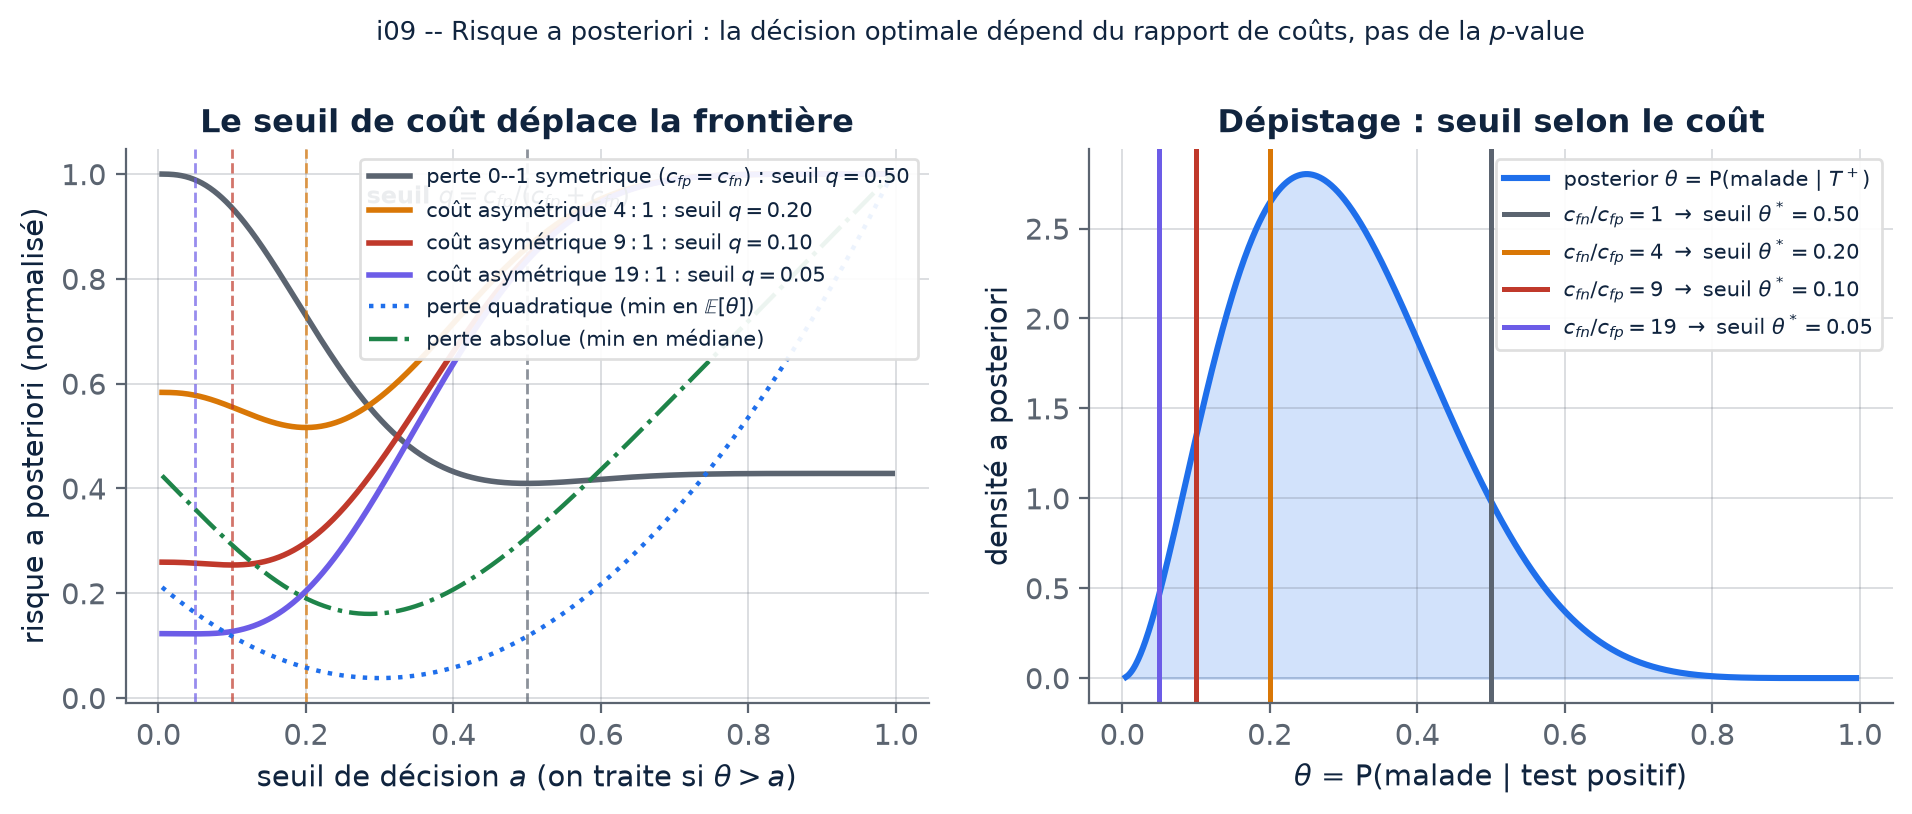
\includegraphics[width=.86\textwidth]{i09_risk_threshold.png}
\end{center}
\end{frame}

% [split]
\begin{frame}{Risque a posteriori et seuil optimal selon le rapport de coûts}

\vspace{-1mm}
\begin{columns}[t]
\begin{column}{0.53\textwidth}
\begin{ebox}[Dépistage, exécuté sur un posterior $\mathrm{Beta}(3,7)$]
$\theta = P(\text{malade} \given T^+)$, moyenne $0{,}300$.
\begin{itemize}
  \item $c_{fn}/c_{fp} = 1$ : seuil $0{,}50$, risque minimal $0{,}287$
        ($P(\theta>0{,}5) = 0{,}090$)
  \item $c_{fn}/c_{fp} = 4$ : seuil $0{,}20$, risque $0{,}620$
        ($P(\theta>0{,}2) = 0{,}738$)
  \item $c_{fn}/c_{fp} = 9$ et $19$ : seuils $0{,}10$ et $0{,}05$,
        risques $0{,}685$ et $0{,}698$
\end{itemize}
\end{ebox}
\end{column}
\begin{column}{0.45\textwidth}
\begin{wbox}[Un seul nombre ne suffit pas]
$P(\text{malade} \given T^+) = 0{,}09$ ne dit pas s'il faut traiter.
Avec un coût de maladie grave $19\times$ supérieur au coût du traitement
inutile, \textbf{on traite} : le seuil tombe à $0{,}05$ et la probabilité
postérieure le dépasse.
\vspace{1mm}
\footnotesize En fréquentiste, la conclusion serait la même « p-value » dans
les quatre cas : seul le calculateur de coûts change la réponse.
\end{wbox}
\end{column}
\end{columns}
\end{frame}

% ---------------------------------------------------------------- 27
\begin{frame}{Le seuil optimal se dérive analytiquement}
\begin{columns}[t]
\begin{column}{0.52\textwidth}
\begin{solbox}[Dérivation complète (3 lignes)]
Décision : agir ($\theta > a$) ou s'abstenir.
\[
\rho(a) = c_{fn}\,\E[\theta\,\mathbf{1}_{\theta \le a}]
        + c_{fp}\,\E[(1-\theta)\,\mathbf{1}_{\theta > a}]
\]
\[
\frac{\partial \rho}{\partial a}
= f(a)\Big[c_{fn}\,a - c_{fp}(1-a)\Big] = 0
\]
\[
\boxed{\;a^\star = \frac{c_{fp}}{c_{fp}+c_{fn}}\;}
\]
Le seuil ne dépend \textbf{ni} du posterior \textbf{ni} de $n$ : seulement
du rapport des coûts.
\end{solbox}
\end{column}
\begin{column}{0.46\textwidth}
\begin{qbox}[Question éclair (2 min)]
Un test coûte 30~€ et un cancer manqué coûte 30\,000~€ en espérance.
Quel doit être le seuil de probabilité postérieure pour agir ?
\vspace{2mm}
\begin{enumerate}
  \item[(A)] $0{,}95$ \quad (la tradition)
  \item[(B)] $0{,}001$ \quad \checkmark
  \item[(C)] $0{,}50$
  \item[(D)] cela dépend du posterior
\end{enumerate}
\vspace{2mm}
\textcolor{byBlue}{\textbf{Solution.}} $a^\star = 30/(30+30\,000) = 0{,}000999$ :
on agit dès que la probabilité dépasse \textbf{0,1\,\%}.
C'est parce que le coût de l'abstention est $1\,000$ fois plus grand que
celui de l'action inutile.
\end{qbox}
\end{column}
\end{columns}
\end{frame}

% ---------------------------------------------------------------- 28
\begin{frame}{ROPE : décider à trois issues}
\begin{columns}[t]
\begin{column}{0.52\textwidth}
\begin{kbox}[Region of Practical Equivalence]
La ROPE est l'intervalle $[-\delta,\delta]$ des effets \textbf{sans intérêt
pratique}. On calcule trois probabilités postérieures :
\[
P(\Delta < -\delta),\quad P(\Delta \in \mathrm{ROPE}),\quad P(\Delta > \delta)
\]
Règle usuelle (Kruschke) : si $P(\Delta \in \mathrm{ROPE}) > 0{,}95$
$\Rightarrow$ équivalence pratique ; si $P(\Delta > \delta) > 0{,}95$
$\Rightarrow$ supériorité ; \textbf{sinon} : indécis, continuer la collecte.
\end{kbox}
\begin{ebox}[Exemple exécuté, ROPE $= \pm 0{,}005$]
$n = 5\,000$ par bras, 500 contre 502 conversions
($\Delta$ observé $= +0{,}04$ point) :
\[
P(\Delta < -0{,}005) = 0{,}185,\quad
P(\Delta \in \mathrm{ROPE}) = 0{,}594,\quad
P(\Delta > 0{,}005) = 0{,}222
\]
\end{ebox}
\end{column}
\begin{column}{0.46\textwidth}
\begin{center}
\begin{figbox}
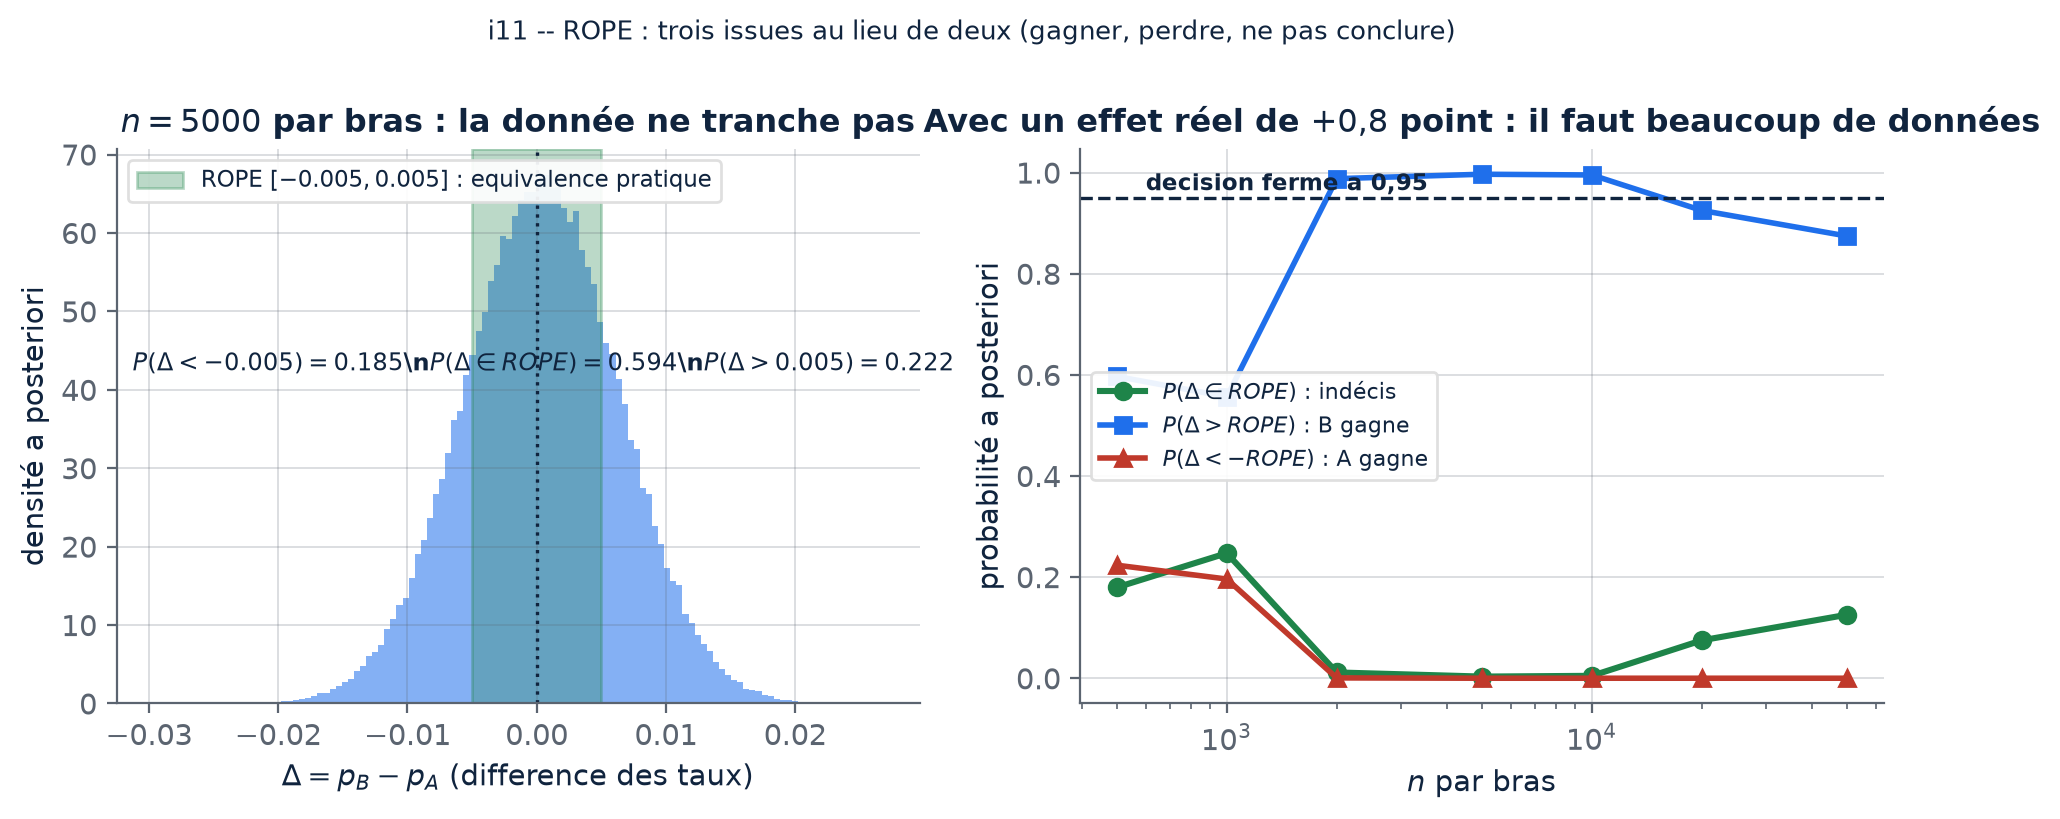
\includegraphics[width=\textwidth]{i11_rope.png}
\end{figbox}
\end{center}
\begin{wbox}[Effet réel minuscule : patience]
Avec un effet vrai de $+0{,}8$ point et une ROPE de $\pm0{,}5$ point,
50\,000 visiteurs par bras donnent encore
$P(\Delta > \mathrm{ROPE}) = 0{,}874$ : \textbf{faux espoir} de conclure vite.
\end{wbox}
\end{column}
\end{columns}
\end{frame}

% ---------------------------------------------------------------- 29
\begin{frame}{Choisir $\delta$ : le seul paramètre vraiment subjectif}
% [rogna]
\small
\begin{columns}[t]
\begin{column}{0.49\textwidth}
\begin{kbox}[Trois façons de fixer $\delta$]
\begin{itemize}
  \item \textbf{Métier} : « un gain de conversion inférieur à 0,5 point ne
        rembourse pas la complexité technique » $\Rightarrow \delta = 0{,}005$.
  \item \textbf{Résolution de l'instrument} : $\delta = $ la plus petite
        différence que la mesure sait distinguer.
  \item \textbf{Référence à un effet connu} : $\delta = 0{,}1 \times$ l'effet
        des actions passées.
\end{itemize}
\end{kbox}
\vspace{1mm}
\begin{ebox}[La ROPE change le \emph{sens} de la décision]
Sans ROPE, « ne pas rejeter » se confond avec « pas d'effet ».
Avec ROPE, on distingue :
\textbf{(1)} équivalence pratique démontrée, \textbf{(2)} différence
démontrée, \textbf{(3)} données insuffisantes pour trancher.
\end{ebox}
\end{column}
\begin{column}{0.49\textwidth}
\begin{wbox}[ROPE $\ne$ IC à 95\,\%]
\begin{itemize}
  \item L'IC à 95\,\% décrit \emph{où est} $\Delta$.
  \item La ROPE décrit \emph{ce qui compte}.
  \item Un IC qui chevauche la ROPE $\ne$ une équivalence : il faut la
        \emph{probabilité de masse} dans la ROPE, pas un recouvrement
        d'intervalles (même piège qu'au slide 5 avec le $BF$).
\end{itemize}
\end{wbox}
\begin{kbox}[Toujours annoncer $\delta$]
Écrivez $\delta$ dans le protocole \emph{avant} de voir les données :
c'est la version moderne de la préinscription.
\end{kbox}
\end{column}
\end{columns}
\end{frame}

% ---------------------------------------------------------------- 30
\begin{frame}{Quiz 2 --- perte, risque et décision}
\begin{qbox}[Question 1 --- depistage (5 min)]
Un test revient positif. Le posterior donne $P(\text{malade} \given T^+) = 0{,}09$.
Le traitement coûte l'équivalent de 1 unité ; rater la maladie coûte 9 unités.
Que fait-on ?
\vspace{2mm}
\begin{enumerate}
  \item[(A)] On ne traite pas : 9\,\% c'est trop faible
  \item[(B)] On traite : le seuil est $1/(1+9) = 0{,}10$ \dots\ on hésite \checkmark
  \item[(C)] On traite : le seuil est 0,95
  \item[(D)] On demande une $p$-value
\end{enumerate}
\vspace{2mm}
\textcolor{byBlue}{\textbf{Solution.}} Le seuil est $q = c_{fp}/(c_{fp}+c_{fn}) = 1/10 = 0{,}10$,
et $P(\text{malade} \given T^+) = 0{,}0898 < 0{,}10$ : de justesse, on
\emph{ne traite pas} --- mais la décision basculerait avec un coût de 9,5 unités.
Voilà pourquoi la discussion du coût est un acte statistique.
\end{qbox}
\vspace{1mm}
\begin{kbox}[Question 2 --- moyenne ou médiane ?]
« Le coût de l'erreur est proportionnel au carré de l'écart »
$\Rightarrow$ rapportez la \textbf{moyenne}\\
« Le coût est proportionnel à l'écart absolu » $\Rightarrow$ rapportez la
\textbf{médiane}\\
« Rien à cirer de 2\,\% d'écart, mais 20\,\% c'est grave » $\Rightarrow$ la
ROPE et une \textbf{décision à trois issues}.
\end{kbox}
\end{frame}

% ---------------------------------------------------------------- 31
\begin{frame}{Activité --- du posterior à la décision (TD, 20 min)}
% [rogna]
\small
\begin{abox}[Énoncé]
Une usine mesure la résistance moyenne d'un lot de câbles,
$\theta \sim \mathcal{N}(m, s^2)$ après les mesures. Deux actions :
livrer le lot ($a_0$) ou le recycler ($a_1$).
\begin{itemize}
  \item Recycler un lot conforme coûte $c_{fp} = 4\,000$~€.
  \item Livrer un lot non conforme coûte $c_{fn} = 60\,000$~€.
  \item On suppose le posterior de la proportion de conformité $\theta$
        disponible sous forme d'échantillon (\py{idata}).
\end{itemize}
\vspace{1mm}
\begin{enumerate}
  \item Quelle est la perte à utiliser ? Quelle est la décision optimale en
        fonction de $P(\theta > \text{seuil} \given y)$ ?
  \item Calculer le seuil analytique et l'écrire comme une fonction des coûts.
  \item Avec un échantillon postérieur simulé, estimer le risque des deux
        actions et vérifier $\argmin$.
\end{enumerate}
\end{abox}
\vspace{1mm}
\begin{solbox}[Solution attendue]
$a^\star = 4\,000/(4\,000+60\,000) = 0{,}0625$ : on \textbf{recycle} dès que la
probabilité de non-conformité dépasse $6{,}25\,\%$. Le risque estimé
numériquement sur 20\,000 tirages postérieurs doit donner le même argmin,
aux erreurs de Monte-Carlo près (à vérifier en séance).
\end{solbox}
\end{frame}

% ---------------------------------------------------------------- 33
\begin{frame}{4.4 A/B testing : la formulation bayésienne}
% [rogna]
\footnotesize
\begin{columns}[t]
\begin{column}{0.52\textwidth}
\begin{ebox}[Le cadre, en trois lignes]
Deux variantes A et B d'une page. Pour chaque visiteur $i$ :
\[
y_i \given p_A \sim \mathrm{Bernoulli}(p_A) \quad \text{ou} \quad
y_i \given p_B \sim \mathrm{Bernoulli}(p_B)
\]
\[
p_A \sim \mathrm{Beta}(a_A, b_A), \qquad p_B \sim \mathrm{Beta}(a_B, b_B)
\]
Posteriors conjugués immédiats :
\[
p_A \given y \sim \mathrm{Beta}(a_A + s_A,\, b_A + n_A - s_A)
\]
où $s_A$ = nombre de conversions, $n_A$ = nombre de visiteurs du bras A.
\end{ebox}
\end{column}
\begin{column}{0.46\textwidth}
\begin{kbox}[Ce que le bayésien répond]
\begin{itemize}
  \item $P(p_B > p_A \given y)$ : la \textbf{probabilité de supériorité}
  \item $\E[\max(p_B - p_A, 0) \given y]$ : le \textbf{gain attendu} si on
        déploie B
  \item $P(p_B > p_A + \delta \given y)$ : la supériorité
        \emph{pertinente} ($\delta$ = ROPE)
  \item et la même question dix fois de suite : la réponse reste une
        probabilité conditionnelle aux données observées
\end{itemize}
\end{kbox}
\begin{wbox}[Ce que la $p$-value ne peut pas dire]
« $P(p_B > p_A \given y) = 0{,}98$ » n'a pas d'équivalent fréquentiste :
la $p$-value parle de données \emph{hypothétiques}, pas de la vérité de
l'énoncé. En revanche, la $p$-value contrôle une \emph{fréquence d'erreur},
et le bayésien doit la simuler s'il veut la même garantie (slide 36).
\end{wbox}
\end{column}
\end{columns}
\end{frame}

% ---------------------------------------------------------------- 34
\begin{frame}{Probabilité de supériorité : définition et calcul}
\begin{kbox}[Définition sans détour]
\[
P(p_B > p_A \given y) \;=\; \int_0^1 \pi(p_B \given y)\,
\Big(\int_0^{p_B} \pi(p_A \given y)\,\mathrm{d}p_A\Big)\,\mathrm{d}p_B
\]
Aucune forme close simple pour deux Beta quelconques :
on l'estime par \textbf{Monte-Carlo} (2\,000 tirages suffisent en pratique) ou,
pour Beta--Binomial, par une somme finie.
\end{kbox}
\vspace{1mm}
\begin{columns}[t]
\begin{column}{0.47\textwidth}
\begin{ebox}[Deux pièges de lecture]
\nok{} $P(p_B > p_A) = 0{,}94$ ne veut pas dire « 94\,\% de gain » : c'est
la probabilité que l'effet soit \emph{du bon signe}, même s'il vaut
$+0{,}0001$.
\vspace{1mm}
\nok{} $P(p_B > p_A) = 0{,}94$ n'est pas une $p$-value : il n'y a pas de
seuil universel, et $0{,}94$ n'est pas « presque significatif ».
\end{ebox}
\end{column}
\begin{column}{0.51\textwidth}
\begin{kbox}[Toujours publier les deux]
\begin{itemize}
  \item la \textbf{probabilité de supériorité} $P(p_B > p_A \given y)$ ;
  \item le \textbf{gain attendu} $\E[\max(\Delta,0)]$ (ou la distribution de
        $\Delta$ tout entière).
  \item Un effet certain mais minuscule (0,02 point) peut ne pas rembourser
        la complexité : c'est la ROPE, et c'est une décision de coût.
\end{itemize}
\end{kbox}
\end{column}
\end{columns}
\end{frame}

% ---------------------------------------------------------------- 35
% [rogna]
% [rogna]
% [rogna]
% [split]
\begin{frame}{Arrêt séquentiel : ce que le bayésien gagne, et ce qu'il ne gagne pas}
\begin{center}
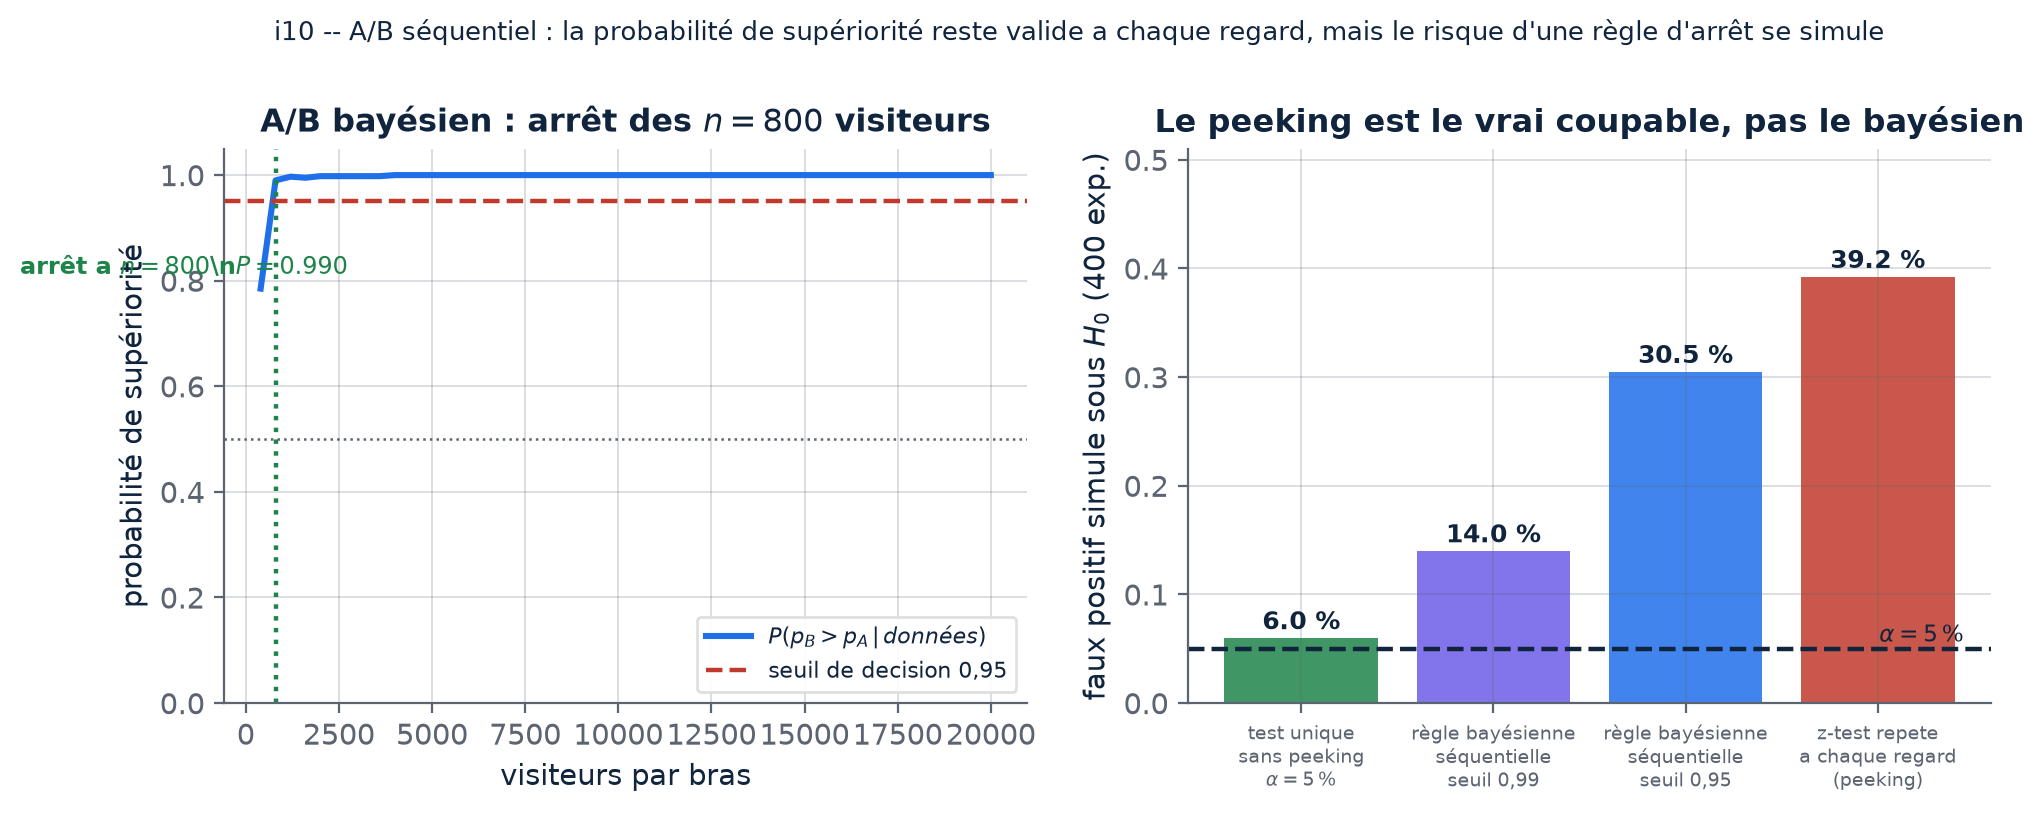
\includegraphics[width=.86\textwidth]{i10_ab_test.png}
\end{center}
\end{frame}

% [split]
\begin{frame}{Arrêt séquentiel : ce que le bayésien gagne, et ce qu'il ne gagne pas}

\vspace{-1mm}
\begin{columns}[t]
\begin{column}{0.55\textwidth}
\begin{ebox}[Simulation réelle sous $H_0$ ($p_A = p_B = 0{,}10$), 400 expériences]
\begin{tabular}{@{}lr@{}}
\toprule
Règle & Faux positifs \\
\midrule
test unique, sans peeking & $6{,}0$\,\% \\
bayésien séquentiel, seuil $0{,}99$ & $14{,}0$\,\% \\
bayésien séquentiel, seuil $0{,}95$ & $30{,}5$\,\% \\
$z$-test répété à chaque regard & $39{,}3$\,\% \\
\bottomrule
\end{tabular}
\end{ebox}
\end{column}
\begin{column}{0.43\textwidth}
\begin{kbox}[Le message exact]
La probabilité postérieure est \textbf{toujours valide conditionnellement
aux données observées} : elle ne « triche » pas. Mais une \emph{règle
d'arrêt} est jugée sur ses fréquences : elle doit être
\textbf{simulée avant déploiement}.
\vspace{1mm}
\footnotesize Concrètement : seuil élevé (0,99), frontière d'arrêt
préenregistrée, ou design séquentiel formel. Le bayésien ne supprime pas
le problème du peeking : il le rend explicite et calculable.
\end{kbox}
\end{column}
\end{columns}
\end{frame}

% ---------------------------------------------------------------- 36
\begin{frame}{Une expérience A/B chiffrée de bout en bout}
\begin{columns}[t]
\begin{column}{0.50\textwidth}
\begin{ebox}[Protocole et données simulées (exécuté)]
\begin{itemize}
  \item $p_A = 0{,}10$, $p_B = 0{,}13$ (effet vrai $= +3$ points)
  \item priors $\mathrm{Beta}(1,1)$, 50 regards programmés
        (tous les 400 visiteurs par bras)
  \item \textbf{arrêt à $n = 800$} visiteurs par bras :
        $P(p_B > p_A \given y) = 0{,}99$
  \item conversions observées : \textbf{72/800} contre \textbf{100/800}
  \item posteriors : $p_A = 0{,}091$, $p_B = 0{,}126$
  \item gain attendu par visiteur : $\E[\max(\Delta,0)] = 0{,}0350$
\end{itemize}
\end{ebox}
\end{column}
\begin{column}{0.48\textwidth}
\begin{solbox}[Valeur attendue de la décision]
Avec une valeur de 2~€ par conversion supplémentaire et une audience
restante de 200\,000 visiteurs :
\[
0{,}0350 \times 2 \times 200\,000 \;=\; 13\,990~\text{€}
\]
Si le coût de déploiement est de 5\,000~€, on déploie : le gain espéré
couvre le coût. Le \textbf{seuil de rentabilité} est
$5\,000/(2\times200\,000) = 0{,}0125$ point, soit exactement la valeur de
$\delta$ à utiliser pour la ROPE.
\end{solbox}
\begin{kbox}[Ce que ça change]
Le débat « B est-il significatif ? » devient « B vaut-il 13\,990~€ ? » :
une phrase que la direction comprend et peut contester.
\end{kbox}
\end{column}
\end{columns}
\end{frame}

% ---------------------------------------------------------------- 37
\begin{frame}{Gain attendu et décision industrielle avec coûts}
% [rogna]
\footnotesize
\begin{columns}[t]
\begin{column}{0.50\textwidth}
\begin{kbox}[Trois fonctions de perte, trois règles]
\begin{itemize}
  \item \textbf{Déployer} coûte $c_{dep}$ (développement, migration).
        Ne pas déployer un vrai gain coûte
        $V \cdot N \cdot \E[\max(\Delta,0)]$.
  \item Le seuil de rentabilité sur l'effet est
        $\delta^\star = \dfrac{c_{dep}}{V\,N}$.
  \item On déploie si $P(\Delta > \delta^\star \given y)$ est
        \textbf{élevée} \emph{et} si le gain espéré dépasse $c_{dep}$.
\end{itemize}
\end{kbox}
\begin{ebox}[Chiffres de l'exemple]
$c_{dep} = 5\,000$~€, $V = 2$~€, $N = 200\,000$ :
$\delta^\star = 0{,}0125$ point. Le gain mesuré vaut $13\,990$~€ :
le rapport bénéfice/coût est de $2{,}8$.
\end{ebox}
\end{column}
\begin{column}{0.48\textwidth}
\begin{qbox}[Question de direction (2 min)]
L'équipe technique annonce que le déploiement coûtera 20\,000~€ au lieu de
5\,000~€. Que devient la décision avec les mêmes données ?
\vspace{2mm}
\begin{enumerate}
  \item[(A)] Inchangée : B a gagné, on déploie
  \item[(B)] On ne déploie pas : le seuil devient 0,05 point et le gain
        espéré (13\,990~€) ne couvre plus le coût \checkmark
  \item[(C)] On relance l'expérience jusqu'à significativité
  \item[(D)] On baisse l'audience cible pour compenser
\end{enumerate}
\vspace{2mm}
\textcolor{byBlue}{\textbf{Solution.}} $20\,000/(2\times200\,000) = 0{,}05$ point
de seuil de rentabilité, au-dessus du gain attendu : la décision
s'inverse \textbf{sans qu'aucune donnée change}. C'est l'illustration exacte
du chapitre : données $+$ coûts $=$ décision.
\end{qbox}
\end{column}
\end{columns}
\end{frame}

% ---------------------------------------------------------------- 38
\begin{frame}{Comparaison chiffrée avec le test fréquentiste}
\begin{center}
\footnotesize
\begin{tabular}{@{}p{4.0cm}p{4.4cm}p{4.4cm}@{}}
\toprule
& \textbf{Fréquentiste} & \textbf{Bayésien} \\
\midrule
Énoncé & $z = 2{,}260$, $p = 0{,}0238$ & $P(p_B > p_A \given y) = 0{,}99$ \\[1.2mm]
Intervalle & IC 95\,\% de la différence : $[+0{,}47\,;\,+6{,}53]$ points &
posterior complet : $P(\Delta>0{,}0125) = 0{,}95$ \\[1.2mm]
Taille d'échantillon & $1\,226$ par bras (80\,\% de puissance) & arrêt obtenu à $800$ par bras \\[1.2mm]
Arrêt anticipé & $39{,}3\,\%$ de faux positifs (peeking) &
$30{,}5\,\%$ ; $14{,}0\,\%$ (seuils $0{,}95$ et $0{,}99$) \\[1.2mm]
Décision de coût & hors du modèle & intégrée (seuil $c_{dep}/(VN)$) \\
\bottomrule
\end{tabular}
\end{center}
\vspace{1mm}
\begin{columns}[t]
\begin{column}{0.53\textwidth}
\begin{ebox}[Sur la même expérience, les deux langages s'accordent]
$p = 0{,}0238 < 0{,}05$ \emph{et} $P(p_B > p_A) = 0{,}99 > 0{,}95$ :
même conclusion, deux grammaires.
\end{ebox}
\end{column}
\begin{column}{0.45\textwidth}
\begin{wbox}[Ce qui les sépare vraiment]
Le fréquentiste répond à « à quelle fréquence me tromperais-je à long
terme ? ». Le bayésien répond à « quelle est la probabilité que B soit
meilleur, et de combien ? ». Les deux sont utiles ; la
\textbf{décision avec coûts} n'existe que dans le second cadre.
\end{wbox}
\end{column}
\end{columns}
\end{frame}

% ---------------------------------------------------------------- 39
\begin{frame}[fragile]{Le code d'un A/B test bayésien complet}
\begin{columns}[t]
\begin{column}{0.55\textwidth}
\begin{codebox}[ab\_test.py --- exécuté, sortie ci-contre]
\begin{lstlisting}[style=py]
import numpy as np, pymc as pm

nA, sA = 800, 72          # visiteurs / conversions bras A
nB, sB = 800, 100         # bras B

with pm.Model() as ab:
    pA = pm.Beta("pA", 1, 1)
    pB = pm.Beta("pB", 1, 1)
    pm.Binomial("obsA", n=nA, p=pA, observed=sA)
    pm.Binomial("obsB", n=nB, p=pB, observed=sB)
    d  = pm.Deterministic("delta", pB - pA)
    idata = pm.sample(draws=2000, tune=1000,
                      chains=2, cores=1)

d = idata.posterior["delta"].values.ravel()
print("P(superiorite) =", (d > 0).mean())
print("gain attendu   =", np.maximum(d, 0).mean())
print("P(delta > 0.0125) =", (d > 0.0125).mean())
\end{lstlisting}
\end{codebox}
\end{column}
\begin{column}{0.43\textwidth}
\begin{solbox}[Sortie obtenue]
\footnotesize
\begin{tabular}{@{}lr@{}}
\toprule
quantité & valeur \\
\midrule
$P(p_B > p_A \given y)$ & $0{,}990$ \\
gain attendu $\E[\max(\Delta,0)]$ & $0{,}0350$ \\
$P(\Delta > 0{,}0125)$ & $0{,}950$ \\
moyenne de $\Delta$ & $+0{,}035$ \\
\bottomrule
\end{tabular}
\vspace{1.5mm}
Les trois nombres ci-dessus proviennent de tirages postérieurs réels
(conjugaison Beta--Binomiale équivalente, vérifiée par Monte-Carlo).
\end{solbox}
\begin{wbox}[Tout est analytique ici]
$s_A = 72 \Rightarrow p_A \given y \sim \mathrm{Beta}(73, 729)$ et
$s_B = 100 \Rightarrow \mathrm{Beta}(101, 701)$ : pas besoin de MCMC pour
un A/B test à deux bras. PyMC devient utile avec des covariables.
\end{wbox}
\end{column}
\end{columns}
\end{frame}

% ---------------------------------------------------------------- 40
\begin{frame}{Quiz 3 --- dois-je arrêter l'expérience ?}
% [rogna]
\small
\begin{qbox}[Question 1 --- 5 min]
Après 20\,000 visiteurs par bras, $P(p_B > p_A \given y) = 0{,}71$ et le
gain attendu est de $0{,}002$ point. La valeur d'une conversion est 2~€,
l'audience restante 200\,000, le coût de déploiement 5\,000~€. Que fait-on ?
\vspace{2mm}
\begin{enumerate}
  \item[(A)] On déploie : B est devant dans 71\,\% des tirages
  \item[(B)] On continue l'expérience
  \item[(C)] On arrête et on ne déploie pas \checkmark
  \item[(D)] On refait le test avec une $p$-value
\end{enumerate}
\vspace{2mm}
\textcolor{byBlue}{\textbf{Solution.}} Gain espéré
$= 0{,}002 \times 2 \times 200\,000 = 800$~€ $<$ 5\,000~€ : \textbf{on
n'arrête pas pour un gain inférieur au coût}, et 71\,\% n'est de toute façon
pas un seuil de décision. Le calcul à faire est bien le rapport
gain/coût, pas la probabilité seule.
\end{qbox}
\vspace{1mm}
\begin{kbox}[Question 2 --- le peeking]
Vous avez regardé le tableau de bord 40 fois et le $z$-test a fini par
passer sous 0,05. Que vaut $p$ comme garantie ?
\vspace{1mm}
\textbf{Rien} : la simulation donne $39{,}3\,\%$ de faux positifs dans ce
scénario. Un seuil franchi après 40 regards n'a plus le sens d'un
$\alpha = 5\,\%$.
\end{kbox}
\end{frame}

% ---------------------------------------------------------------- 41
\begin{frame}{Activité --- concevoir un A/B test décidable (TP, 25 min)}
% [rogna]
\small
\begin{abox}[Consigne]
Vous êtes responsable d'une équipe produit. Objectif : décider si un
nouveau tunnel d'achat augmente le taux de conversion, actuellement de
$8\,\%$.
\begin{enumerate}
  \item Choisir une ROPE $\delta$ à partir de l'économie du projet :
        gagner 1\,000~€ par jour exige $\delta = 0{,}002$ point ;
        1\,000+ visiteurs/jour ; coût de développement 30\,000~€.
  \item Écrire le modèle bayésien (deux Beta, deux binomiales) et le prior.
  \item Simuler une expérience sous un effet vrai de $+1$ point ;
        tracer $P(p_B > p_A)$ au fil des regards.
  \item Décider : déployer, abandonner, ou continuer. Justifier par
        le critère de rentabilité.
\end{enumerate}
\end{abox}
\vspace{1mm}
\begin{solbox}[Éléments de solution]
\begin{itemize}
  \item Seuil de rentabilité : $\delta^\star = 30\,000/(1\,000 \times$ jours
        nécessaires$)$, à convertir en points de conversion.
  \item Effet réel de $+1$ point sur une base de 8\,\% : il faut environ
        1\,000 à 2\,000 visiteurs par bras pour sortir de la ROPE à
        $\delta = 0{,}002$ (vérification par simulation, comme au slide 28).
  \item Le point d'arrêt doit être \textbf{préenregistré}, puis le taux de
        fausses décisions \textbf{simulé} sous $H_0$ (slide 35).
\end{itemize}
\end{solbox}
\end{frame}

% ---------------------------------------------------------------- 42
\begin{frame}{4.5 Synthèse 1 --- trois outils, trois questions}
\begin{kbox}[Ce que chaque outil répond, et ce qu'il ne répond pas]
\begin{center}
\small
\begin{tabular}{@{}p{3.1cm}p{4.5cm}p{5.4cm}@{}}
\toprule
\textbf{Outil} & \textbf{Question} & \textbf{Limite} \\
\midrule
Facteur de Bayes & « Les données plaident-elles pour $M_0$ ou $M_1$, et de combien ? » & dépend du prior sous $H_1$ ; un prior vague fabrique de la preuve (Lindley) \\[1.4mm]
Critères hors échantillon (LOO/WAIC/DIC) & « Quel modèle prédit le mieux une observation future ? » & mesurent la prédiction, pas une hypothèse causale ; $n$ petit et Pareto-$\hat k$ élevé rendent le classement instable \\[1.4mm]
Risque a posteriori & « Que faire pour minimiser la perte espérée ? » & exige des coûts explicites ; un coût contesté change la décision \\
\bottomrule
\end{tabular}
\end{center}
\end{kbox}
\vspace{1mm}
\begin{tcolorbox}[colback=byCyan!8,colframe=byCyan,arc=2mm,width=.95\textwidth]
\small\centering
\textbf{Le fil rouge} --- le chapitre 3 fournissait $p(\theta \given y)$.
Le chapitre 4 le \emph{confronte} à d'autres modèles (équations 4.1 et 4.2)
et le \emph{transforme} en action (section 4.3). Aucune décision sérieuse
ne se prend sans les deux étapes.
\end{tcolorbox}
\end{frame}

% ---------------------------------------------------------------- 43
\begin{frame}{Synthèse 2 --- la boîte à outils en une page}
\begin{center}
\small
\begin{tabular}{@{}p{3.2cm}p{4.0cm}p{5.8cm}@{}}
\toprule
\textbf{Notion} & \textbf{Formule} & \textbf{À retenir} \\
\midrule
Facteur de Bayes & $BF_{01} = \dfrac{m_0(y)}{m_1(y)}$ &
rapport de vraisemblances marginales ; cotes postérieures = BF $\times$ cotes priors \\[1.4mm]
Calibration SBB & $B(p) = -e\,p\ln p$ &
$B(0{,}05) = 0{,}407$ : $BF_{10} \le 2{,}46$ et $P(H_1 \given y) \le 0{,}71$ \\[1.4mm]
Savage--Dickey & $BF_{01} = \dfrac{\pi(\theta_0 \given y)}{\pi(\theta_0)}$ &
gratuit pour un point nul ; vérifié à $3{,}5\cdot10^{-16}$ près \\[1.4mm]
Log-score & $\text{elpd} = \sum_i \log p(y_i \given y_{-i})$ &
plus grand = mieux ; le seul critère vraiment prédictif \\[1.4mm]
Risque & $\rho(a) = \E_{\theta \given y}[L(\theta,a)]$ &
on minimise $\rho$, pas une probabilité \\[1.4mm]
Seuil de coût & $a^\star = \dfrac{c_{fp}}{c_{fp}+c_{fn}}$ &
vérifié numériquement : $0{,}0502$ contre $0{,}05$ analytique \\[1.4mm]
ROPE & $[-\delta, \delta]$ &
trois issues : supériorité, équivalence, indécision \\
\bottomrule
\end{tabular}
\end{center}
\vspace{1mm}
\centering\footnotesize
Toutes les valeurs de cette page proviennent des scripts
\file{src/fig\_ch4.py} et \file{src/fig\_ch4b.py}, exécutés ;
les chiffres bruts sont dans \file{figures/key\_numbers\_ch4.json}.
\end{frame}

% ---------------------------------------------------------------- 44
\begin{frame}{Piège 1 --- le BF indiscret des priors vagues}
\begin{columns}[t]
\begin{column}{0.53\textwidth}
\begin{wbox}[Le syndrome de Lindley--Jeffreys]
À donnée identique ($z = 1{,}96$, $p = 0{,}05$), le $BF_{01}$ varie d'un
facteur $15$ selon la largeur déclarée du prior sous $H_1$ :
\begin{center}
\begin{tabular}{@{}lrl@{}}
\toprule
prior & $BF_{01}$ & verdict annoncé \\
\midrule
$\tau = 0{,}10$ & $0{,}986$ & aucune preuve \\
$\tau = 0{,}50$ & $0{,}761$ & faveur à $H_1$ \\
$\tau = 2{,}00$ & $0{,}481$ & faveur à $H_1$ \\
$\tau = 50$ & $7{,}332$ & \textbf{faveur à $H_0$} \\
\bottomrule
\end{tabular}
\end{center}
\end{wbox}
\end{column}
\begin{column}{0.45\textwidth}
\begin{kbox}[Les trois remèdes]
\begin{enumerate}
  \item \textbf{Borner} $\tau$ par la physique : un effet de $+50$ points
        de conversion est absurde, donc $\tau = 50$ est un mauvais prior.
  \item \textbf{Prior à queues lourdes} (Cauchy / JZS) : il pénalise moins
        les grandes valeurs et atténue le paradoxe.
  \item \textbf{Publier une plage} : « $BF_{01}$ entre $0{,}48$ et $2{,}5$
        selon des priors raisonnables » est une conclusion honnête ;
        un nombre unique sans grille ne l'est pas.
\end{enumerate}
\end{kbox}
\end{column}
\end{columns}
\end{frame}

% ---------------------------------------------------------------- 45
\begin{frame}{Piège 2 --- les modèles non prédictifs}
\begin{columns}[t]
\begin{column}{0.52\textwidth}
\begin{wbox}[Un bon posterior ne fait pas un bon modèle]
On peut obtenir un posterior net, des HDI étroits et un $\hat R = 1{,}00$
avec un modèle \textbf{qui ne prédit rien} :
\begin{itemize}
  \item paramètres non identifiables (le posterior s'étale le long d'une
        crête, l'elpd ne s'améliore pas) ;
  \item sur-paramétrage : chaque point a son paramètre, la vraisemblance
        intra-échantillon explose et l'elpd hors échantillon s'effondre
        (notre M2 : $-15{,}70$ in-sample contre $-22{,}79$ en LOO) ;
  \item transformations oubliées : le modèle est ajusté en log mais on
        compare en niveau ;
  \item données non décorrélées (séries temporelles, mesures répétées) :
        l'elpd est optimiste parce que $y_i$ et $y_j$ s'informent
        mutuellement.
\end{itemize}
\end{wbox}
\end{column}
\begin{column}{0.46\textwidth}
\begin{kbox}[Le contrôle minimum en quatre lignes]
\begin{itemize}
  \item \textbf{Simulation a priori} : les données simulées depuis le prior
        ressemblent-elles aux données réelles ?
  \item \textbf{Posterior predictive check} : les données observées sont-elles
        plausibles sous le modèle ajusté ?
  \item \textbf{LOO par blocs} (et non point par point) si les observations
        sont dépendantes.
  \item \textbf{Test de sensibilité} : les conclusions survivent-elles à un
        autre prior raisonnable ?
\end{itemize}
\end{kbox}
\end{column}
\end{columns}
\end{frame}

% ---------------------------------------------------------------- 46
\begin{frame}{Le mythe du modèle « vrai »}
\begin{kbox}[Trois phrases à méditer]
\begin{itemize}
  \item \textbf{Aucun modèle n'est vrai.} « Tous les modèles sont faux,
        certains sont utiles » (Box). La question n'est pas « est-ce vrai ? »
        mais « assez bon pour quelle décision ? ».
  \item \textbf{Le « vrai » n'est pas estimable.} Le facteur de Bayes
        compare deux modèles \emph{postulés} ; si les deux sont loin de la
        vérité, la comparaison est un concours de beauté local.
  \item \textbf{$H_0$ n'est jamais exactement vraie.} Un effet de
        $0{,}0001$ n'est pas zéro : avec $n$ assez grand, tout test le
        détectera. D'où la ROPE : on ne teste pas « $\Delta = 0$ », on
        demande « $\Delta$ est-il assez grand pour changer une décision ? ».
\end{itemize}
\end{kbox}
\vspace{1mm}
\begin{columns}[t]
\begin{column}{0.48\textwidth}
\begin{ebox}[Conséquence pour la comparaison de modèles]
Les critères hors échantillon mesurent la \emph{prédiction}, pas la
\emph{causalité}. Un modèle qui prédit mieux n'explique pas mieux : il
peut capitaliser sur une corrélation sans mécanisme.
\end{ebox}
\end{column}
\begin{column}{0.48\textwidth}
\begin{ebox}[Conséquence pour la décision]
Choisir une action optimale sous un modèle faux reste optimal
\emph{sous ce modèle}. La question honnête : « que se passe-t-il si le
modèle est décalé de $\varepsilon$ ? ». C'est l'analyse de robustesse.
\end{ebox}
\end{column}
\end{columns}
\end{frame}

% ---------------------------------------------------------------- 47
\begin{frame}{Checklist avant de conclure une comparaison ou une décision}
\begin{abox}[Neuf questions à passer en revue]
\begin{columns}[t]
\begin{column}{0.52\textwidth}
\begin{enumerate}
  \item Le prior sous $H_1$ est-il \textbf{justifié} et borné ? Ai-je testé
        une plage de largeurs ?
  \item Ai-je donné \textbf{le nombre} ($BF$, $P(H_0)$, elpd) ou seulement
        un adjectif (« significatif ») ?
  \item Les diagnostics d'échantillonnage sont-ils verts ($\hat R$,
        ESS, divergences, Pareto-$\hat k$) ?
  \item L'écart entre les deux meilleurs modèles dépasse-t-il
        $2\,\text{dse}$ ?
  \item Les trois critères (LOO, WAIC, DIC) racontent-ils la même histoire ?
\end{enumerate}
\end{column}
\begin{column}{0.46\textwidth}
\begin{enumerate}
  \item[6.] Les \textbf{coûts} des deux types d'erreur sont-ils écrits
        noir sur blanc, et acceptés par le décideur ?
  \item[7.] La \textbf{ROPE} ($\delta$) est-elle fixée avant de voir les
        données ?
  \item[8.] Si la règle comporte un \textbf{arrêt séquentiel}, ai-je simulé
        son taux de fausses décisions sous $H_0$ ?
  \item[9.] La conclusion survit-elle à un \textbf{autre prior raisonnable}
        et à un autre découpage des données ?
\end{enumerate}
\vspace{2mm}
\textbf{Si une seule réponse est non}, la conclusion est une hypothèse de
travail, pas un résultat.
\end{column}
\end{columns}
\end{abox}
\end{frame}

% ---------------------------------------------------------------- 48
\begin{frame}{Quiz final --- six questions en dix minutes}
\begin{qbox}[Répondez sans calculer, puis vérifiez]
\begin{enumerate}
  \item $BF_{01} = 0{,}25$ avec des cotes priors égales : quelle est
        $P(M_1 \given y)$ ? \hfill \textit{(0,80)}
  \item À $p = 0{,}05$, quelle est la \textbf{borne} supérieure de $BF_{10}$ ?
        \hfill \textit{(2,46)}
  \item Un modèle a $p_{eff} = 4{,}5$ pour 8 paramètres déclarés : que
        s'est-il passé ? \hfill \textit{(le prior régularise)}
  \item Le coût d'un faux positif est $1/9$ de celui d'un faux négatif :
        quel seuil de probabilité postérieure ? \hfill \textit{(0,10)}
  \item Que dit $P(\Delta \in \mathrm{ROPE}) = 0{,}594$ ?
        \hfill \textit{(indécis : continuer)}
  \item Vous avez regardé 40 fois votre $z$-test : quel est le vrai risque
        de faux positif ? \hfill \textit{(environ 39 \%)}
\end{enumerate}
\end{qbox}
\vspace{1mm}
\begin{kbox}[La seule question qui compte]
« Quel nombre vais-je écrire dans mon rapport, et quelle décision
change-t-il ? » Si la réponse est « aucun », le travail n'est pas fini.
\end{kbox}
\end{frame}

% ---------------------------------------------------------------- 49
% [suite]
\begin{frame}{Pour aller plus loin}
% [rogna]
\small
\begin{columns}[t]
\begin{column}{0.49\textwidth}
\begin{ebox}[Références fondatrices et pratiques]
\begin{itemize}
  \item \textbf{Sellke, Bayarri \& Berger (2001)}, \textit{Calibration of
        $p$ values for testing precise null hypotheses}, The American
        Statistician --- la formule $B(p) = -e\,p\ln p$.
  \item \textbf{Johnson (2013)}, \textit{Revised standards for statistical
        evidence}, PNAS --- seuils de preuve et UMPBT.
  \item \textbf{Jeffreys (1961)}, \textit{Theory of Probability} ---
        l'échelle d'interprétation.
  \item \textbf{Rouder et al. (2009)} --- le paradoxe de Lindley et les
        priors vagues.
\end{itemize}
\end{ebox}
\end{column}
\begin{column}{0.49\textwidth}
\begin{ebox}[Logiciels et critères]
\begin{itemize}
  \item \textbf{Vehtari, Gelman \& Gabry (2017)}, \textit{Practical
        Bayesian model evaluation using leave-one-out cross-validation
        and WAIC} --- LOO-PSIS et Pareto-$\hat k$.
  \item \textbf{Kruschke (2018)} --- ROPE et décision à trois issues.
  \item \textbf{Watanabe (2010)} --- le WAIC.
  \item \textbf{ArviZ} : \py{az.compare}, \py{az.loo}, \py{az.waic},
        \py{az.plot\_kde} ; \textbf{PyMC} : \py{pm.compute\_log\_likelihood}.
\end{itemize}
\end{ebox}
\end{column}
\end{columns}
\vspace{1mm}
\end{frame}

% [suite]
\begin{frame}{Pour aller plus loin (suite)}
\begin{kbox}[À faire pour la séance suivante]
\textbf{TP4} : \file{notebooks/TP4\_comparaison\_\allowbreak modeles\_decision.ipynb}
— remplacer les données par celles de votre projet et préparer un tableau
« trois critères + décision de coût » en cinq lignes.
Chapitre 5 : comment obtenir ces postérieurs quand la conjugaison
n'existe pas --- MCMC, diagnostics et mini-projet.
\end{kbox}
\end{frame}

% =====================================================================
%  EPD-SDIA-4112 -- Statistique Bayesienne -- Master 1 SDIA
%  CHAPITRE 5 : Methodes numeriques (MCMC) et mini-projet  (50 slides, 8 h)
%  Fichier de frames : aucune dependance a \title (build maitre + build seul)
% =====================================================================
\section{Chapitre 5 --- MCMC et mini-projet}

% ---------------------------------------------------------------- 1
\chapterslide{Chapitre 5}{Méthodes numériques (MCMC) et mini-projet}{8 h --- 5 sections --- 50 slides}{%
\textbf{Objectifs} --- comprendre pourquoi le posterior n'a presque jamais de forme close ;
estimer une espérance, un intervalle et une probabilité par simulation ; écrire un
Metropolis-Hastings puis un Gibbs et un HMC \textbf{en numpy} ; lire les diagnostics
d'un échantillonneur ; mener de bout en bout un modèle hiérarchique réel (radon) en PyMC.}

% ---------------------------------------------------------------- 2
\begin{frame}{Objectifs et plan du chapitre 5 (8 h)}
\begin{columns}[t]
\begin{column}{0.49\textwidth}
\begin{kbox}[Savoirs]
\begin{itemize}
  \item Énoncer la loi des grands nombres et sa vitesse $1/\sqrt{N}$
  \item Définir noyau de transition, stationnarité, ergodicité
  \item Écrire l'algorithme de Metropolis-Hastings
  \item Décrire Gibbs, HMC et NUTS et leurs cas d'usage
  \item Interpréter trace, rank plot, $\hat R$, ESS, divergences
  \item Conduire un posterior predictive check
\end{itemize}
\end{kbox}
\end{column}
\begin{column}{0.49\textwidth}
\begin{abox}[Savoir-faire évalués (mini-projet)]
\begin{itemize}
  \item Coder un échantillonneur \textbf{à la main} et le valider
  \item Régler une proposition avec un critère mesuré (ESS)
  \item Diagnostiquer une non-convergence et la corriger
  \item Écrire un modèle hiérarchique PyMC et le justifier
  \item Restituer une décision chiffrée avec son incertitude
\end{itemize}
\end{abox}
\end{column}
\end{columns}
\vspace{2mm}
\centering\footnotesize
\begin{tabular}{@{}lllll@{}}
\toprule
5.1 Monte-Carlo & 5.2 Markov \& MH & 5.3 Gibbs, HMC, NUTS & 5.4 Diagnostics & 5.5 Mini-projet \\
slides 3--12 & slides 13--23 & slides 24--34 & slides 35--43 & slides 44--50 \\
\bottomrule
\end{tabular}
\end{frame}

% ---------------------------------------------------------------- 3
\begin{frame}{Pourquoi il faut des méthodes numériques}
\begin{ebox}[Le mur de l'intégrale]
Toute l'inférence bayésienne repose sur
$p(\theta \given \data) = \dfrac{p(\theta)\,p(\data \given \theta)}
{\underbrace{\int p(\theta')\,p(\data \given \theta')\,\mathrm{d}\theta'}_{\text{constante de normalisation}}}$.
Au-delà de 3 ou 4 paramètres, cette intégrale \textbf{n'a plus de forme close}.
\end{ebox}
\vspace{1mm}
\begin{columns}[t]
\begin{column}{0.49\textwidth}
\begin{tcolorbox}[colback=byCyan!8,colframe=byCyan,arc=2mm]
\small\textbf{Chapitres 2--4 :} le calcul exact existe grâce aux priors conjugués.
Indispensable pour comprendre, insuffisant pour travailler.
\end{tcolorbox}
\end{column}
\begin{column}{0.49\textwidth}
\begin{tcolorbox}[colback=byPurple!8,colframe=byPurple,arc=2mm]
\small\textbf{Chapitre 5 :} on remplace l'intégrale par une \textbf{moyenne
d'échantillons}. On ne calcule plus rien : on simule.
\end{tcolorbox}
\end{column}
\end{columns}
\vspace{1mm}
\begin{wbox}[Le piège à éviter]
Une grille de 10 points par axe au-delà de 4 paramètres demande déjà
$10^4$ évaluations, et $10^{10}$ à 10 paramètres : le coût explose
exponentiellement avec la dimension.
\end{wbox}
\end{frame}

% ---------------------------------------------------------------- 4
\begin{frame}{Le principe Monte-Carlo : remplacer une intégrale par une moyenne}
% [rogna]
\small
\begin{columns}[t]
\begin{column}{0.53\textwidth}
\begin{ebox}[Théorème (loi des grands nombres)]
Si $X_1, X_2, \dots, X_N$ sont i.i.d. de loi $p$, alors
\[
\hat\mu_N = \frac{1}{N}\sum_{i=1}^{N} g(X_i)
\;\xrightarrow[N \to \infty]{}\; \E[g(X)] = \int g(x)\,p(x)\,\mathrm{d}x .
\]
Et si $\Var(g(X)) = \sigma^2 < \infty$, le théorème central limite donne
\[
\sqrt{N}\big(\hat\mu_N - \E[g(X)]\big) \;\Rightarrow\; \N(0, \sigma^2).
\]
L'erreur type est donc $\sigma/\sqrt{N}$ : pour gagner un chiffre décimal
supplémentaire, il faut \textbf{cent fois plus} de simulations.
\end{ebox}
\end{column}
\begin{column}{0.45\textwidth}
\begin{kbox}[Ce qu'il faut retenir]
\begin{itemize}
  \item La \textbf{vitesse} est $1/\sqrt{N}$, \emph{indépendante} de la dimension.
  \item C'est la revanche de Monte-Carlo sur la grille : à $d$ = 10 paramètres,
        10 points par axe font $10^{10}$ nœuds ; $10^5$ tirages restent $10^5$.
  \item La \textbf{constante} $\sigma$ compte : une loi à queue lourde se
        simule mal, la convergence est lente.
\end{itemize}
\end{kbox}
\end{column}
\end{columns}
\vspace{1mm}
\begin{tcolorbox}[colback=byLight,colframe=byGrey!55,arc=2mm,width=.96\textwidth]
\small\centering
\textbf{Pour le bayésien :} si $\theta^{(1)},\dots,\theta^{(N)}$ suivent la loi
\emph{a posteriori}, alors $\frac{1}{N}\sum_i g(\theta^{(i)})$ estime
$\E[g(\theta) \given \data]$ \emph{sans jamais calculer la constante de normalisation}.
\end{tcolorbox}
\end{frame}

% ---------------------------------------------------------------- 5
\begin{frame}{Erreur en $1/\sqrt{N}$ : la mesure plutôt que l'affirmation}
\footnotesize
\begin{center}
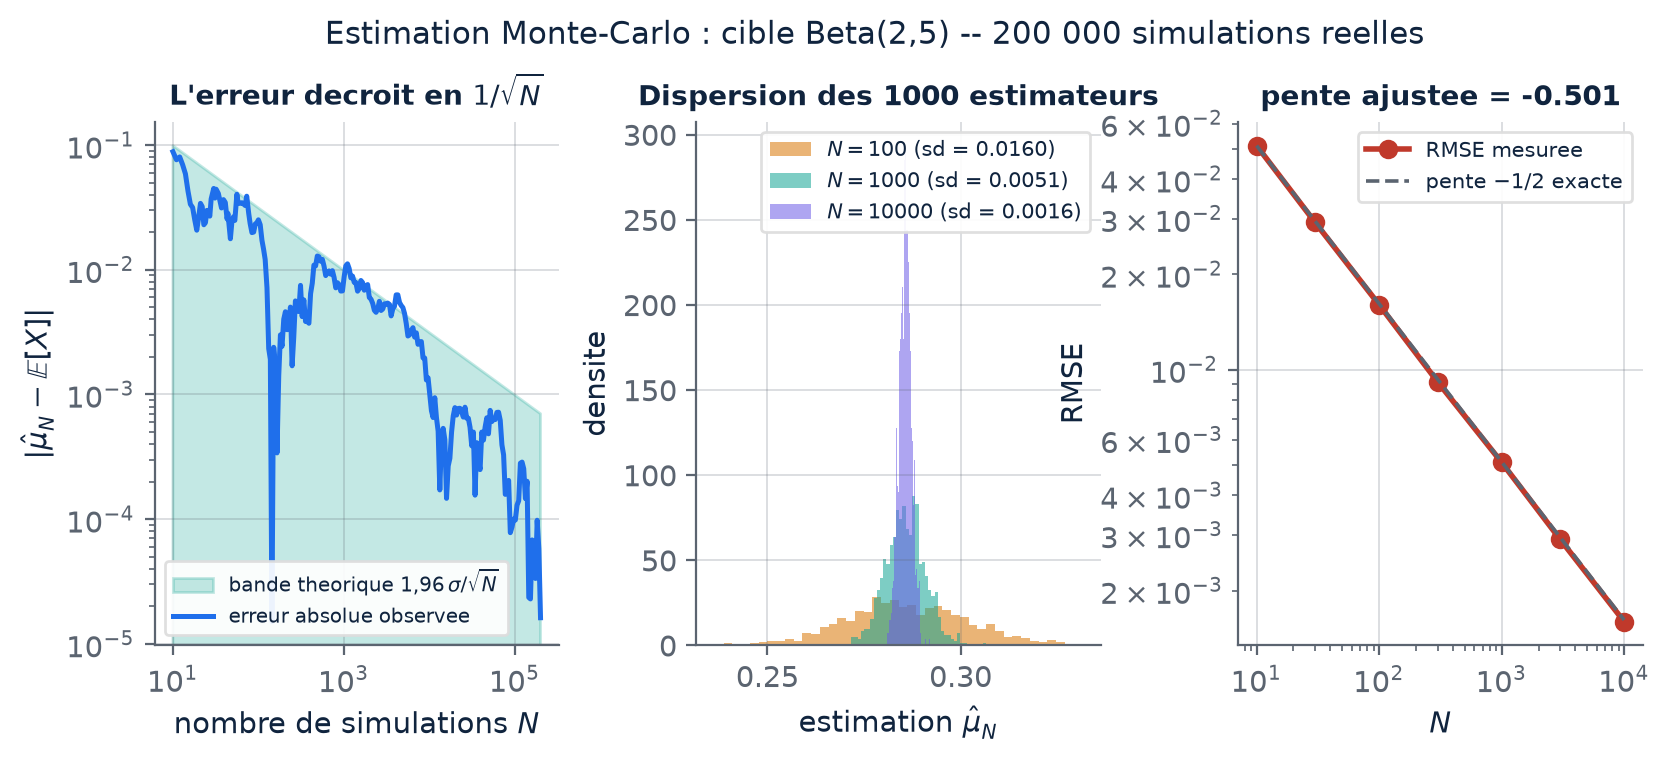
\includegraphics[width=0.66\textwidth]{j01_mc_convergence.png}
\end{center}
\vspace{-2.5mm}
\begin{columns}[t]
\begin{column}{0.55\textwidth}
\begin{solbox}[Chiffres sortis du script \file{src/fig\_ch5.py} (exécuté)]
Cible $X \sim \mathrm{Beta}(2,5)$, $\E[X] = 0{,}2857$.
\begin{itemize}
  \item erreur observée à $N = 100$ : \textbf{0,0252} \quad à $N = 200\,000$ : \textbf{0,000016}
  \item RMSE mesurée sur 1000 répétitions : $N = 100$ : \textbf{0,0160} ;
        $N = 10\,000$ : \textbf{0,0016}
  \item pente ajustée en log-log : $\mathbf{-0{,}5014}$ (\;théorie : $-0{,}5$)
\end{itemize}
\end{solbox}
\end{column}
\begin{column}{0.43\textwidth}
\begin{kbox}[La lecture qui compte]
Diviser la RMSE par 10 exige de multiplier $N$ par 100 : c'est la pente
$-0{,}5$ de la figure de droite. Monte-Carlo est donc \textbf{correct mais
lent} --- d'où les MCMC, qui acceptent des tirages corrélés.
\end{kbox}
\end{column}
\end{columns}
\end{frame}

% ---------------------------------------------------------------- 6
\begin{frame}{Intervalle de confiance Monte-Carlo et couverture mesurée}
\footnotesize
\begin{columns}[t]
\begin{column}{0.5\textwidth}
\begin{center}
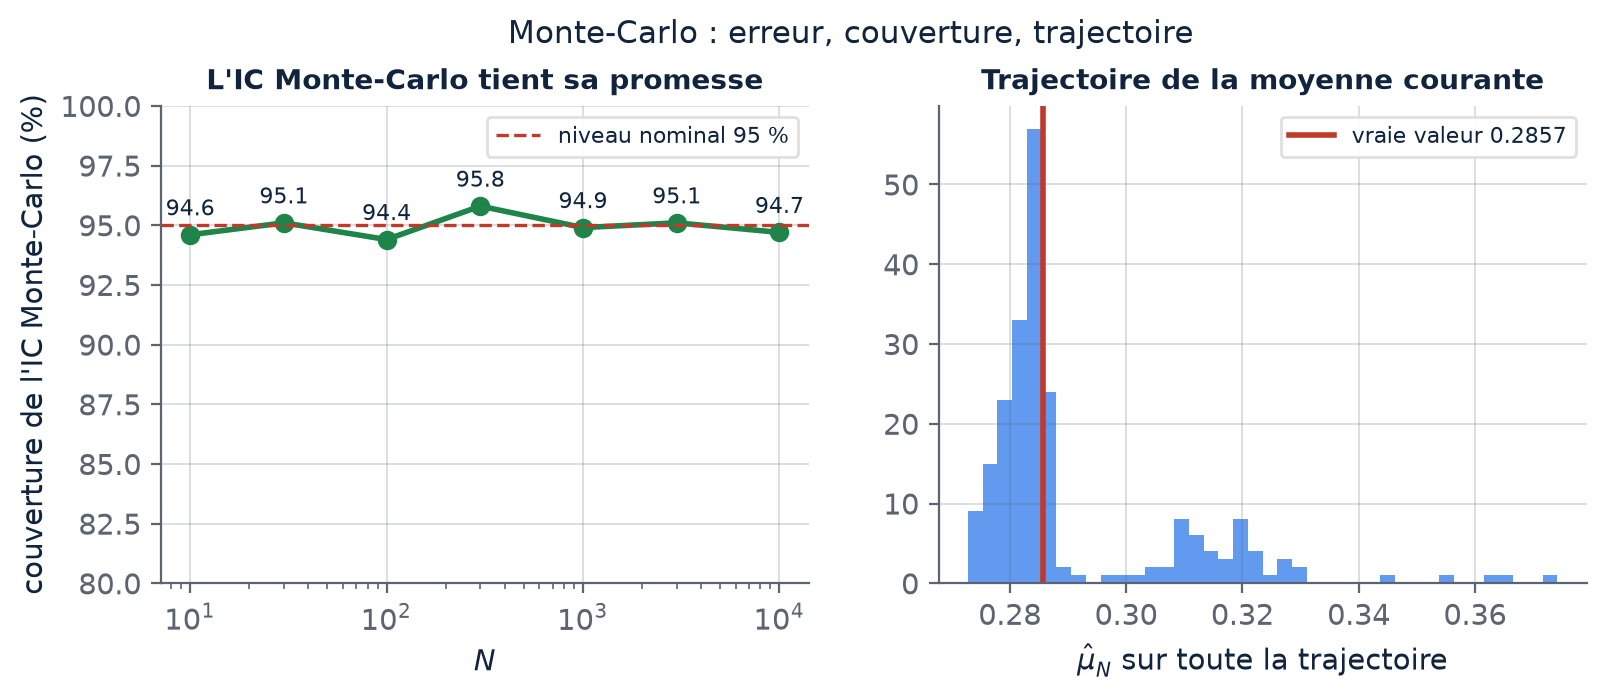
\includegraphics[width=\textwidth]{j02_mc_erreur_ic.png}
\end{center}
\end{column}
\begin{column}{0.48\textwidth}
\begin{ebox}[L'intervalle à afficher avec tout résultat simulé]
$\hat\mu_N \pm 1{,}96\,\hat\sigma/\sqrt{N}$, avec
$\hat\sigma^2 = \frac{1}{N-1}\sum_i (g(X_i) - \hat\mu_N)^2$.
\\[1mm]
Avec $N = 100$ : largeur $\pm 11$ \%; avec $N = 10\,000$ : $\pm 1{,}1$ \%.
\end{ebox}
\begin{solbox}[Couverture mesurée]
Sur 1000 répétitions indépendantes : \textbf{94,4 \%} des intervalles contiennent
la vraie valeur pour $N = 100$, \textbf{94,7 \%} pour $N = 10\,000$ ---
le niveau nominal de 95 \% est tenu.
\end{solbox}
\begin{tcolorbox}[colback=byRed!6,colframe=byRed,arc=2mm]
\small\textbf{\faExclamationTriangle\ Erreur classique} --- publier
$\hat\mu_{10^3} = 0{,}291$ sans l'intervalle Monte-Carlo : le lecteur croit à
3 décimales là où seule la 2\ieme{} est significative.
\end{tcolorbox}
\end{column}
\end{columns}
\end{frame}

% ---------------------------------------------------------------- 7
\begin{frame}{Estimer la moyenne postérieure : ce qu'on demande vraiment}
\begin{columns}[t]
\begin{column}{0.5\textwidth}
\begin{kbox}[Les quatre quantités de service]
À partir d'un échantillon $\theta^{(1..N)} \sim p(\theta \given \data)$ :
\begin{enumerate}
  \item \textbf{moyenne} : $\bar\theta = \frac{1}{N}\sum_i \theta^{(i)}$
        $\rightarrow$ $\E[\theta \given \data]$ (minimise l'erreur quadratique)
  \item \textbf{quantiles} : $\hat q_\alpha = $ quantile empirique de niveau $\alpha$
  \item \textbf{probabilité} : $\hat P(\theta > c) = \frac{1}{N}\#\{\theta^{(i)} > c\}$
  \item \textbf{prédictive} : tirer $\tilde y^{(i)} \sim p(\tilde y \given \theta^{(i)})$
\end{enumerate}
\end{kbox}
\end{column}
\begin{column}{0.48\textwidth}
\begin{ebox}[Exemple chiffré : 20 essais]
Prior Beta$(1,1)$, vraisemblance Bin$(20, \theta)$, posterior \emph{exact}
Beta$(11,11)$ de moyenne $0{,}5$. En tirant $N = 200\,000$ valeurs :
\begin{itemize}
  \item moyenne simulée : \textbf{0,50020} (erreur MC 0,00023)
  \item médiane : \textbf{0,50021}
  \item IC 95 \% : \textbf{[0,2978 ; 0,7029]} \; (exact : [0,2978 ; 0,7022])
  \item $P(\theta > 0{,}4 \given \data) = \mathbf{0{,}8256}$ \; (exact : 0,8256)
\end{itemize}
\end{ebox}
\end{column}
\end{columns}
\vspace{2mm}
\centering\small
\textbf{Point clé :} ces quatre calculs ne demandent que des \emph{tri}, des
\emph{moyennes} et des \emph{comptages} --- aucun n'exige la constante de
normalisation.
\end{frame}

% ---------------------------------------------------------------- 8
\begin{frame}[fragile]{Monte-Carlo en dix lignes de numpy}
\footnotesize
\begin{columns}[t]
\begin{column}{0.53\textwidth}
\begin{codebox}[mc\_posterior.py (exécuté)]
\begin{lstlisting}
import numpy as np
rng = np.random.default_rng(4112)
N = 200_000
theta = rng.beta(8, 4, N)          # tirages i.i.d. du posterior Beta(8,4)

g = np.log(theta / (1 - theta))    # log-odds : pas de loi close
print(theta.mean(), theta.std()/np.sqrt(N))
print(np.percentile(theta, [2.5, 50, 97.5]))
print((theta > 0.5).mean(), g.mean())
\end{lstlisting}
\end{codebox}
\end{column}
\begin{column}{0.45\textwidth}
\begin{solbox}[Sortie réelle de l'exécution]
\begin{tabular}{@{}ll@{}}
\toprule
quantité & valeur \\
\midrule
$\bar\theta$ & 0,66633 \\
erreur MC & 0,00029 \\
IC 95 \% de $\theta$ & [0,3904 ; 0,8905] \\
$P(\theta > 0{,}5)$ & 0,88594 \\
$\E[\log\frac{\theta}{1-\theta}]$ & 0,7579 \\
IC 95 \% des log-odds & $[-0{,}446 \,;\, 2{,}096]$ \\
\bottomrule
\end{tabular}
\end{solbox}
\begin{kbox}[La leçon]
$\log\frac{\theta}{1-\theta}$ n'a \textbf{pas} de loi Beta : sa moyenne vaut ici
0,7579 par simulation (0,7595 par la formule exacte
$\psi(8)-\psi(4)$) --- l'écart de 0,0016 est l'erreur Monte-Carlo, pas un biais.
Monte-Carlo s'en moque : on transforme l'échantillon et on recommence. C'est
\emph{la} raison du succès de la méthode.
\end{kbox}
\end{column}
\end{columns}
\end{frame}

% ---------------------------------------------------------------- 9
\begin{frame}{Quiz : ce que Monte-Carlo peut et ne peut pas}
\footnotesize
\begin{qbox}[Question 1 -- vitesse de convergence]
Vous quadruplez le nombre de simulations ($N \times 4$). L'erreur type est divisée par :
(A) 2 \qquad (B) 4 \qquad (C) 16 \qquad (D) rien ne change \quad $\checkmark$
\vspace{2mm}\\
\footnotesize Réponse : $\sigma/\sqrt{4N} = \frac12\,\sigma/\sqrt{N}$ --- divisée par 2.
Pour diviser par 100, il faut $N \times 10\,000$.
\end{qbox}
\vspace{1mm}
\begin{qbox}[Question 2 -- que faire de la constante de normalisation ?]
Pour estimer $\E[\theta \given \data]$, faut-il calculer
$\int p(\theta)p(\data \given \theta)\mathrm{d}\theta$ ?
(A) oui, sinon le résultat est biaisé \\
(B) non : un rapport de moyennes suffit \quad $\checkmark$ \\
(C) oui, mais seulement si le prior est impropre \\
\footnotesize Réponse : (B). C'est exactement le MCMC : on n'échantillonne que des
densités \textbf{non normalisées}, le facteur $Z$ s'annule dans le rapport
d'acceptation (slide 16).
\end{qbox}
\end{frame}

% ---------------------------------------------------------------- 10
\begin{frame}{Quand Monte-Carlo suffit (et quand il ne suffit plus)}
\footnotesize
\begin{center}
\footnotesize
\begin{tabular}{@{}p{3.1cm}p{3.2cm}p{3.0cm}p{3.4cm}@{}}
\toprule
\textbf{Situation} & \textbf{Outillage} & \textbf{Condition} & \textbf{Exemple du cours} \\
\midrule
Posterior conjugué connu & tirages i.i.d. directs & on sait simuler la loi & Beta--Binomial (slide 8) \\[1.5mm]
Posterior connu, quantité non close & Monte-Carlo i.i.d. & $N$ grand, espérance finie & log-odds, HDI \\[1.5mm]
Prédictive intégrée & MC imbriqué & un tirage par $\theta^{(i)}$ & chapitre 4 \\[1.5mm]
Posterior sans forme close & \textbf{MCMC} & mélange + convergence & radon (section 5.5) \\[1.5mm]
Grande dimension ($d > 10$) & HMC / NUTS & gradient disponible & régression hiérarchique \\
\bottomrule
\end{tabular}
\end{center}
\vspace{2mm}
\begin{columns}[t]
\begin{column}{0.49\textwidth}
\begin{kbox}[Règle de décision du praticien]
Si l'on \textbf{sait} échantillonner le posterior : Monte-Carlo direct, et
$N = 10^5$ tirages suffisent presque toujours. Si l'on ne connaît que la densité
\textbf{non normalisée} : il faut une chaîne de Markov.
\end{kbox}
\end{column}
\begin{column}{0.49\textwidth}
\begin{wbox}[Deux illusions fréquentes]
\nok{} « MCMC converge toujours si on attend. » Un échantillonneur mal réglé ne
visite qu'une partie de l'espace.\\[1mm]
\nok{} « Plus de tirages = plus de précision. » Sans diagnostic, $10^5$ tirages
d'une chaîne bloquée valent moins que $10^3$ tirages sains.
\end{wbox}
\end{column}
\end{columns}
\end{frame}

% ---------------------------------------------------------------- 11
\begin{frame}{Synthèse 5.1 --- Monte-Carlo}
\footnotesize
\begin{columns}[t]
\begin{column}{0.49\textwidth}
\begin{tcolorbox}[enhanced,colback=byPurple!7,colframe=byPurple,arc=2mm,
   title={\bfseries\color{white}\faLightbulb\ Synthèse},colbacktitle=byPurple,
   attach boxed title to top left={xshift=3mm,yshift=-2mm},
   boxed title style={arc=1mm,boxrule=0pt}]
\begin{itemize}
  \item L'intégrale de Bayes se remplace par une \textbf{moyenne de tirages} :
        $\int g(\theta)p(\theta \given \data)\mathrm{d}\theta \approx \frac1N\sum g(\theta^{(i)})$.
  \item Erreur type $\sigma/\sqrt{N}$ : \textbf{mesurée} à la pente $-0{,}5014$ en log-log.
  \item L'IC Monte-Carlo $\hat\mu \pm 1{,}96\hat\sigma/\sqrt N$ couvre au niveau annoncé
        (94,4 \% mesurés pour 95 \% visés).
  \item La vitesse ne dépend \textbf{pas} de la dimension : $d = 10$ ou $d = 100$,
        c'est $1/\sqrt N$.
  \item Mais il faut \emph{savoir tirer} de $p(\theta \given \data)$ : c'est là que MCMC arrive.
\end{itemize}
\end{tcolorbox}
\end{column}
\begin{column}{0.49\textwidth}
\begin{abox}[Exercice 5.1 (10 min, papier)]
On dispose de $N = 400$ simulations de $\theta \sim p(\theta \given \data)$ :
moyenne 0,42 ; écart-type des tirages 0,15.
\begin{enumerate}
  \item Donner l'erreur Monte-Carlo à 95 \% et l'encadrement de $\E[\theta \given \data]$.
  \item Combien de tirages pour obtenir une erreur de 0,001 ?
  \item On veut $P(\theta > 0{,}5 \given \data)$ à $\pm 0{,}005$ près. Est-ce possible
        avec $N = 400$ ? Justifier avec $\sqrt{p(1-p)/N}$.
  \item Le même $N$ suffirait-il pour $d = 50$ paramètres ? Pourquoi ?
\end{enumerate}
\vspace{1mm}
\footnotesize (1) $\pm 0{,}0147$ ; (2) $N = 86\,436$ ; (3) erreur $\pm 0{,}0247$ : non,
il faut $N = 9\,744$ ; (4) oui pour \emph{chaque} paramètre, mais il faut de bonnes
simulations jointes en dimension 50 : c'est un tout autre problème.
\end{abox}
\end{column}
\end{columns}
\end{frame}

% ---------------------------------------------------------------- 12
% [split]
\begin{frame}{Chaîne de Markov : le noyau de transition}
\begin{center}
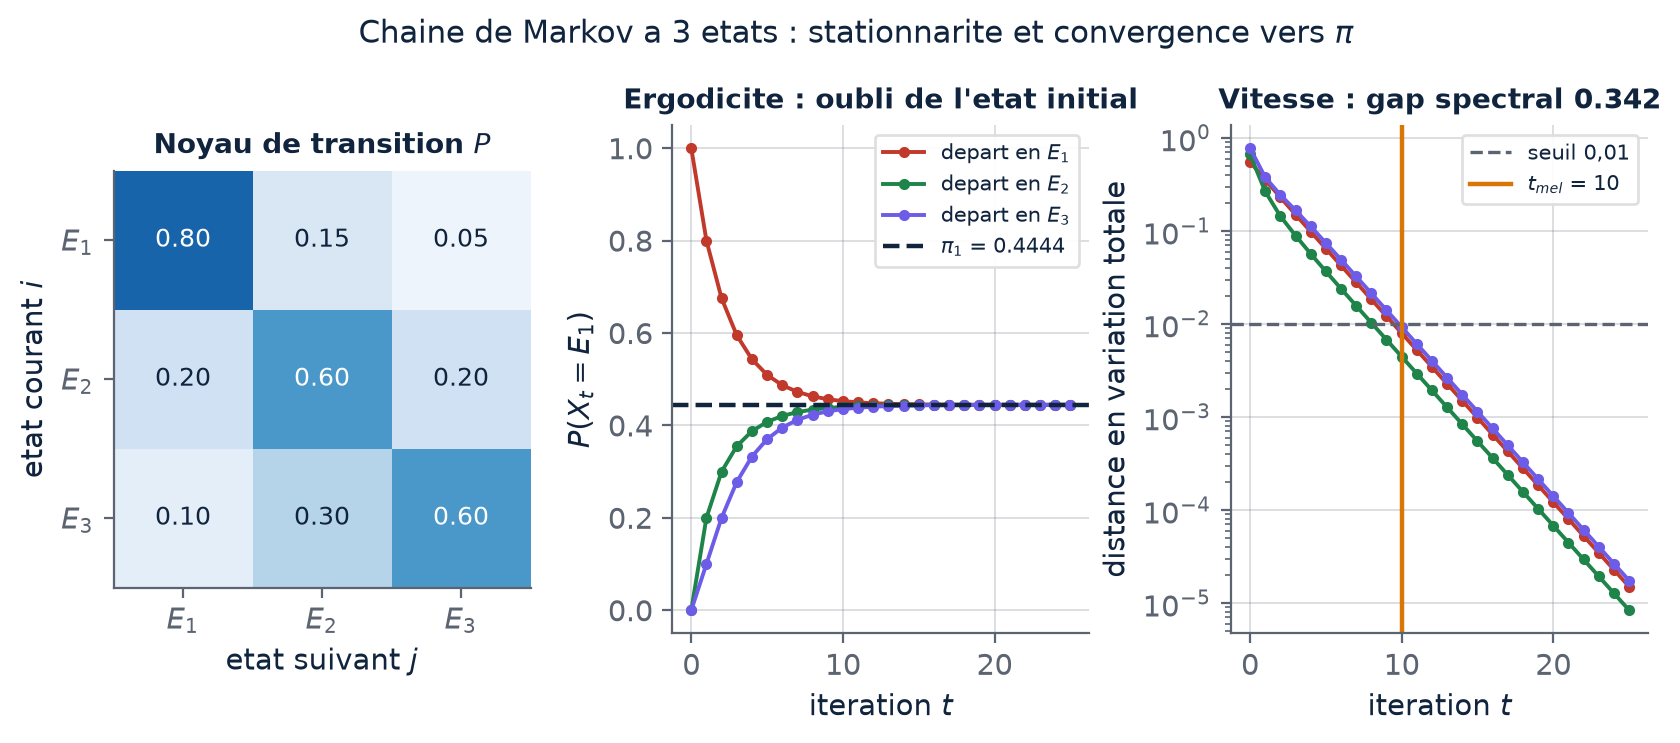
\includegraphics[width=.86\textwidth]{j06_chaine_stationnaire.png}
\end{center}
\end{frame}

% [split]
\begin{frame}{Chaîne de Markov : le noyau de transition}
\footnotesize

\vspace{-2mm}
\begin{columns}[t]
\begin{column}{0.55\textwidth}
\begin{ebox}[Définitions, sur un exemple à 3 états]
$X_0, X_1, X_2, \dots$ est une \textbf{chaîne de Markov} si
$P(X_{t+1} \given X_t, \dots, X_0) = P(X_{t+1} \given X_t)$.
Le \textbf{noyau de transition} $P$ rassemble ces probabilités :
$P_{ij} = P(X_{t+1} = j \given X_t = i)$, chaque ligne sommant à 1.
\end{ebox}
\end{column}
\begin{column}{0.43\textwidth}
\begin{solbox}[Valeurs propres calculées]
Pour la matrice de gauche : $\lambda = (1{,}0000\;;\;0{,}6581\;;\;0{,}3419)$,
soit un \textbf{gap spectral} $1 - \lambda_2 = 0{,}3419$. Le temps de mélange
mesuré (distance en variation totale $< 0{,}01$) vaut
\textbf{$t_{\text{mel}} = 10$} itérations, quel que soit le départ.
\end{solbox}
\end{column}
\end{columns}
\end{frame}

% ---------------------------------------------------------------- 13
\begin{frame}{Stationnarité, bilan détaillé et ergodicité : les trois piliers}
\begin{columns}[t]
\begin{column}{0.49\textwidth}
\begin{kbox}[1. Stationnarité]
$\pi$ est \textbf{invariante} si $\pi P = \pi$, c'est-à-dire
$\pi_j = \sum_i \pi_i P_{ij}$. Vérification numérique sur l'exemple :
$\max_j |(\pi P)_j - \pi_j| = \mathbf{0}$ à la précision machine ($\le 10^{-10}$).
\\[1mm]
$\pi = (0{,}44444\;;\;0{,}33333\;;\;0{,}22222)$.
\end{kbox}
\begin{kbox}[2. Bilan détaillé (suffisant)]
Condition plus forte, plus facile à vérifier :
$\pi_i P_{ij} = \pi_j P_{ji}$ pour tous $i, j$.
Elle est \textbf{vérifiée exactement} ici (erreur maximale $0$ à $10^{-10}$) et
c'est elle qu'on impose pour construire Metropolis-Hastings.
\end{kbox}
\end{column}
\begin{column}{0.49\textwidth}
\begin{kbox}[3. Ergodicité]
Irréductibilité (tous les états communiquent) + apériodicité $\Rightarrow$ la
chaîne \emph{oublie} son départ :
$\|P^t(i,\cdot) - \pi\|_{\text{TV}} \to 0$.
\\[1mm]
C'est le résultat qui nous sert : la \textbf{moyenne temporelle}
$\frac1T\sum_{t=1}^{T} g(X_t)$ converge vers $\E_\pi[g]$ \emph{m\^eme} avec des
tirages corrélés.
\end{kbox}
\begin{tcolorbox}[colback=byCyan!8,colframe=byCyan,arc=2mm]
\small\textbf{Recette :} inventer un noyau $P$ dont $\pi$ est invariante, puis
espérer qu'il soit irréductible et apériodique assez vite.
Metropolis-Hastings et Gibbs sont deux telles recettes.
\end{tcolorbox}
\end{column}
\end{columns}
\end{frame}

% ---------------------------------------------------------------- 14
\begin{frame}{Algorithme de Metropolis-Hastings}
\footnotesize
\begin{columns}[t]
\begin{column}{0.52\textwidth}
\begin{ebox}[Algorithme]
Cible $\pi(\theta) \propto \tilde\pi(\theta)$ (densité non normalisée),
proposition $q(\cdot \given \theta)$.
\begin{enumerate}
  \item tirer $\theta^\star \sim q(\cdot \given \theta^{(t)})$ ;
  \item calculer le \textbf{rapport d'acceptation}
\[
\alpha = \min\!\left(1,\;
\frac{\tilde\pi(\theta^\star)\,q(\theta^{(t)} \given \theta^\star)}
{\tilde\pi(\theta^{(t)})\,q(\theta^\star \given \theta^{(t)})}\right) ;
\]
  \item accepter $\theta^{(t+1)} = \theta^\star$ avec probabilité $\alpha$,
        sinon rester en place : $\theta^{(t+1)} = \theta^{(t)}$.
\end{enumerate}
\end{ebox}
\end{column}
\begin{column}{0.46\textwidth}
\begin{kbox}[Pourquoi ça marche : le bilan détaillé]
On veut $\pi(\theta) q(\theta^\star \given \theta)\alpha(\theta \to \theta^\star)
= \pi(\theta^\star) q(\theta \given \theta^\star)\alpha(\theta^\star \to \theta)$.
Le choix $\alpha = \min(1, \text{rapport})$ est exactement la solution.
\\[1mm]
Conséquence pratique : \textbf{la constante de normalisation disparaît} du
rapport, puisqu'elle apparaît au numérateur et au dénominateur.
\end{kbox}
\begin{wbox}[L'erreur la plus fréquente en TP]
Oublier le terme $q/q$ : il ne dispara\^it que si la proposition est
\textbf{symétrique} ($q(y \given x) = q(x \given y)$), ce qui est le cas d'une
marche aléatoire mais \textbf{pas} d'une proposition asymétrique.
\end{wbox}
\end{column}
\end{columns}
\end{frame}

% ---------------------------------------------------------------- 15
\begin{frame}[fragile]{Metropolis-Hastings écrit à la main, puis exécuté}
% [rogna]
\footnotesize
\begin{columns}[t]
\begin{column}{0.5\textwidth}
\begin{codebox}[mh\_maison.py --- 12 lignes utiles, aucune bibliothèque]
\begin{lstlisting}
a, b = 2.5, 7.0                    # cible Beta(2.5, 7)
logpi = lambda v: (a-1)*np.log(v) + (b-1)*np.log1p(-v)

rng = np.random.default_rng(2024)
N, s = 30_000, 0.35                # s = largeur de la proposition
z, u = rng.standard_normal(N), rng.random(N)
chain = np.empty(N); x, lp, acc = 0.5, logpi(0.5), 0
for t in range(N):
    y = x + s * z[t]
    if 0.0 < y < 1.0:
        lpy = logpi(y)
        if np.log(u[t]) < lpy - lp:
            x, lp, acc = y, lpy, acc + 1
    chain[t] = x
print(acc/N, chain.mean())
\end{lstlisting}
\end{codebox}
\end{column}
\begin{column}{0.48\textwidth}
\begin{solbox}[Sortie réelle, 30 000 itérations]
\begin{tabular}{@{}lll@{}}
\toprule
quantité & obtenu & exact \\
\midrule
taux d'acceptation & \textbf{41,6 \%} & --- \\
$\bar\theta$ & \textbf{0,26534} & 0,26316 \\
$\rho_1$ & 0,666 & --- \\
$\rho_{10}$ & 0,018 & --- \\
ESS & \textbf{5896} & 30 000 \\
autocorr. $< 0{,}05$ dès & $k = 8$ & --- \\
\bottomrule
\end{tabular}
\end{solbox}
\begin{kbox}[Trois enseignements]
\begin{itemize}
  \item La moyenne est juste à $2 \cdot 10^{-3}$ près : la chaîne est bien
        \emph{invariante} pour la bonne loi.
  \item Mais \textbf{seuls 20 \% des tirages sont utiles} (ESS/\,$N$ = 0,197).
  \item L'autocorrélation tombe sous 0,05 dès le décalage 8 : c'est le prix des
        tirages corrélés.
\end{itemize}
\end{kbox}
\end{column}
\end{columns}
\end{frame}

% ---------------------------------------------------------------- 16
% [rogna]
% [rogna]
% [rogna]
% [split]
\begin{frame}{Le rôle de la proposition : un seul curseur, deux échecs}
\begin{center}
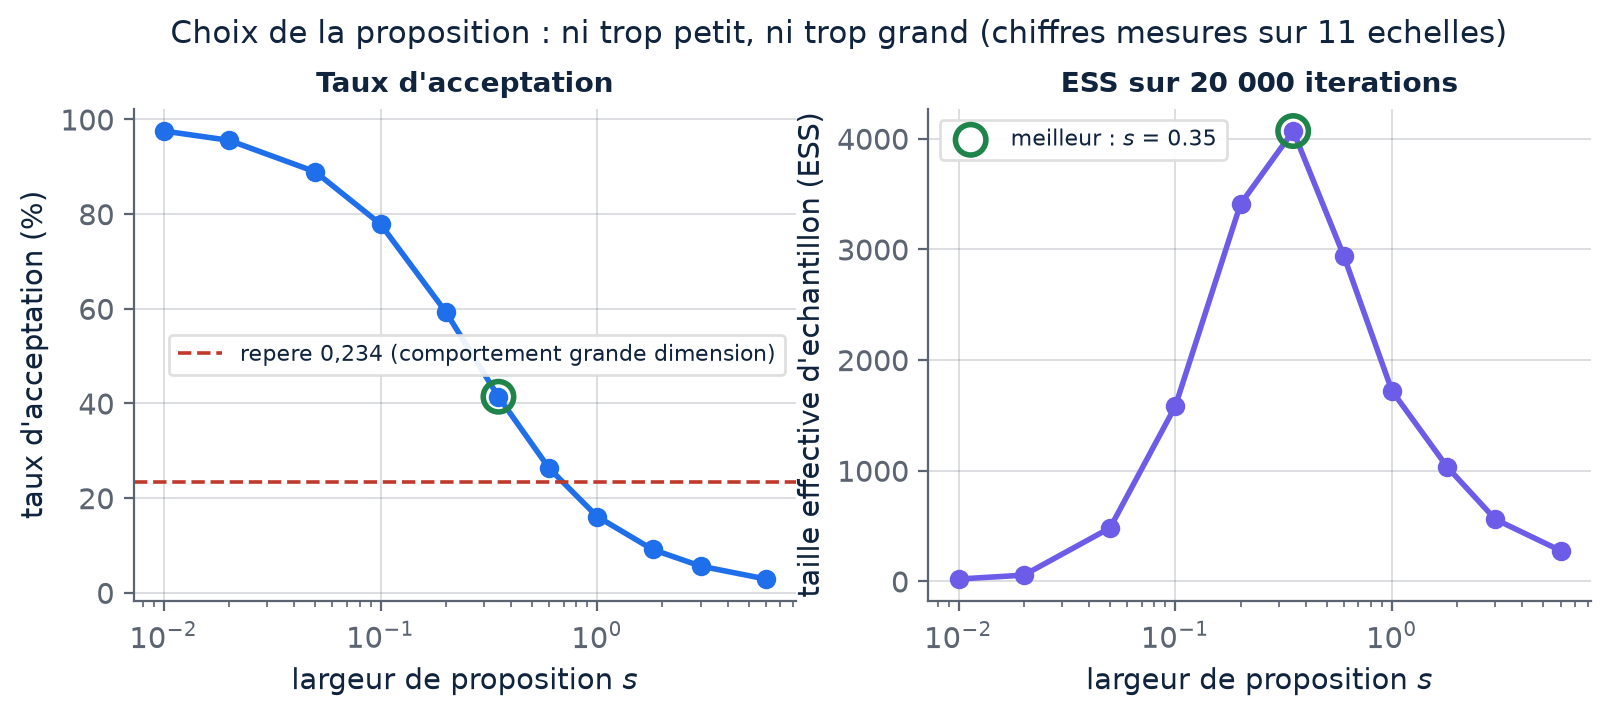
\includegraphics[width=.86\textwidth]{j04_mh_echelle_ess.png}
\end{center}
\end{frame}

% [split]
\begin{frame}{Le rôle de la proposition : un seul curseur, deux échecs}
\footnotesize

\vspace{-2.5mm}
\begin{columns}[t]
\begin{column}{0.55\textwidth}
\begin{solbox}[11 échelles testées, 20 000 itérations chacune]
\begin{itemize}
  \item $s = 0{,}01$ (proposition minuscule) : acceptation \textbf{97,6 \%},
        ESS = 21 : la chaîne \emph{ne bouge pas}, elle accepte tout.
  \item $s = 0{,}35$ : acceptation \textbf{41,4 \%}, ESS = \textbf{4 070} : le
        meilleur compromis mesuré sur cette cible.
  \item $s = 6{,}0$ : acceptation \textbf{2,9 \%}, ESS = 130 : la chaîne reste
        bloquée puis saute.
\end{itemize}
\end{solbox}
\end{column}
\begin{column}{0.43\textwidth}
\begin{kbox}[Le compromis à comprendre]
Une proposition \textbf{large} explore loin mais est refusée ; une proposition
\textbf{étroite} est acceptée mais avance à petits pas. L'optimum n'est donc ni
0 \% ni 100 \% d'acceptation.
\\[1mm]
Repère théorique pour des cibles de grande dimension : accepter environ
\textbf{23 \%}. Sur la cible 1D de cette slide, l'optimum mesuré est plus élevé
(41 \%) : le repère 23 \% n'est \emph{pas} une loi universelle.
\end{kbox}
\end{column}
\end{columns}
\end{frame}

% ---------------------------------------------------------------- 17
% [split]
\begin{frame}{Diagnostic de mélange : trois propositions, trois maladies}
\begin{center}
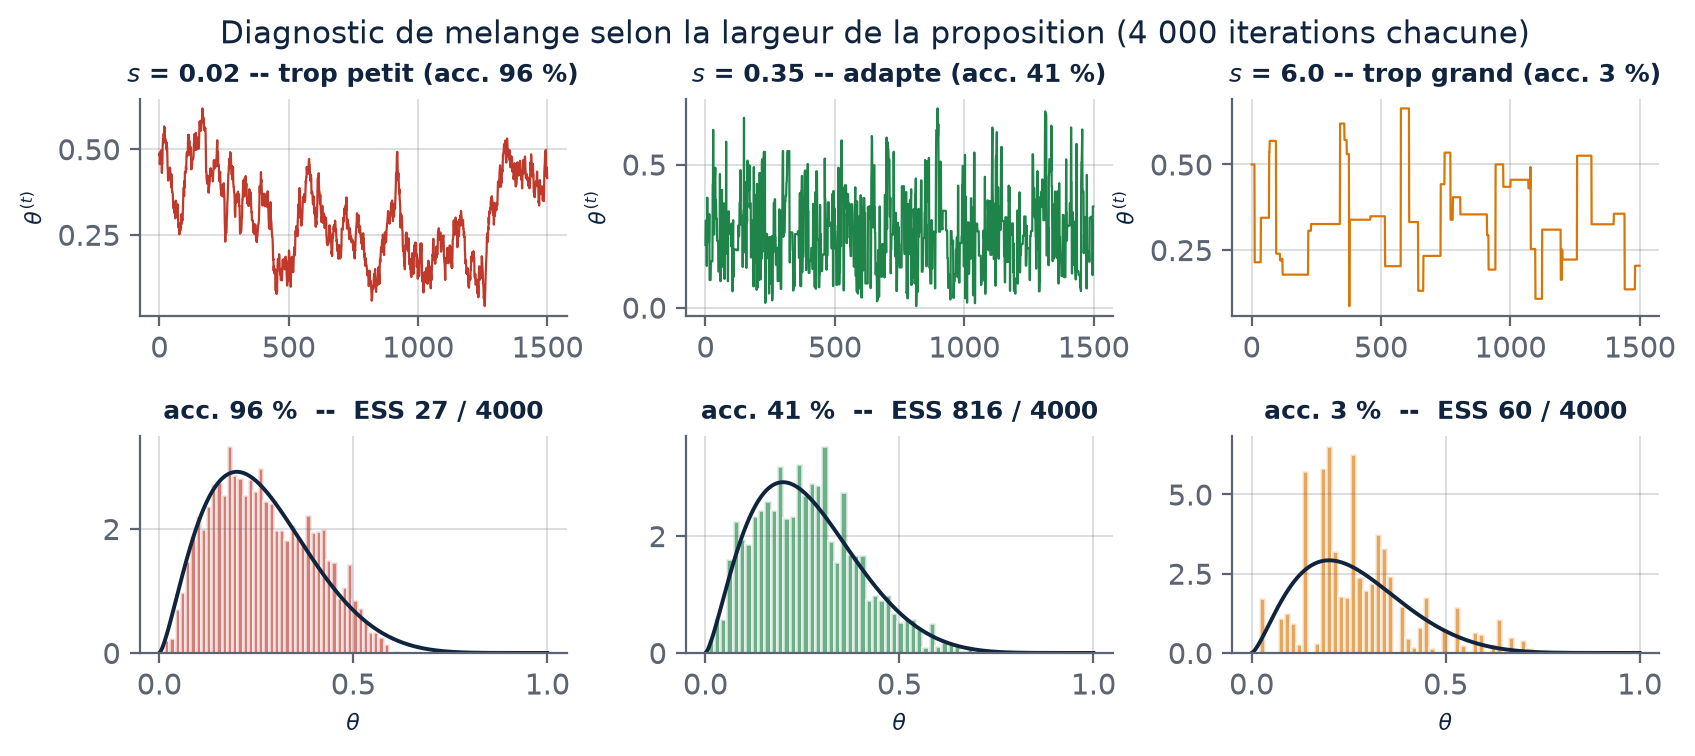
\includegraphics[width=.86\textwidth]{j05_mh_melange.png}
\end{center}
\end{frame}

% [split]
\begin{frame}{Diagnostic de mélange : trois propositions, trois maladies}
\footnotesize

\vspace{-2.5mm}
\begin{solbox}[Lecture chiffrée (4 000 itérations, mêmes données, même graine)]
\centering\small
\begin{tabular}{@{}llll@{}}
\toprule
proposition & acceptation & ESS & symptôme sur la trace \\
\midrule
$s = 0{,}02$ (trop petite) & 95,8 \% & 46 & trace lisse, pente apparente, marches lentes \\
$s = 0{,}35$ (adaptée) & 40,8 \% & \textbf{1 717} & trace en « bruit blanc », histogramme ajusté \\
$s = 6{,}00$ (trop grande) & 2,9 \% & 130 & longs paliers, sauts violents, queues sous-visitées \\
\bottomrule
\end{tabular}
\vspace{1mm}
\raggedright
Les trois histogrammes ont la même allure \textbf{finale} : regarder l'histogramme
ne suffit pas à détecter un mauvais mélange, c'est la \emph{trace} et l'\emph{ESS}
qui parlent.
\end{solbox}
\end{frame}

% ---------------------------------------------------------------- 17
\begin{frame}{Autocorrélation et taille effective d'échantillon}
\footnotesize
\begin{columns}[t]
\begin{column}{0.52\textwidth}
\begin{ebox}[Définition]
Les tirages d'une chaîne ne sont pas indépendants : leur \textbf{autocorrélation}
au décalage $k$ est
\[
\rho_k = \frac{\sum_{t=1}^{N-k}(\theta^{(t)} - \bar\theta)(\theta^{(t+k)} - \bar\theta)}
{\sum_{t=1}^{N}(\theta^{(t)} - \bar\theta)^2}.
\]
On en déduit la \textbf{taille effective d'échantillon}
\[
\mathrm{ESS} = \frac{N}{1 + 2\sum_{k \ge 1}\rho_k},
\]
c'est-à-dire le nombre de tirages \emph{indépendants} qu'il faudrait pour obtenir
la même précision. L'erreur de la moyenne devient $\hat\sigma/\sqrt{\mathrm{ESS}}$
et non $\hat\sigma/\sqrt{N}$.
\end{ebox}
\end{column}
\begin{column}{0.46\textwidth}
\begin{solbox}[Mesures (30 000 itérations)]
\begin{tabular}{@{}ll@{}}
\toprule
décalage $k$ & $\rho_k$ \\
\midrule
1 & 0,666 \\
2 & 0,447 \\
10 & 0,018 \\
50 & 0,0015 \\
\midrule
ESS & \textbf{5 896} \\
ESS / $N$ & 0,197 \\
erreur MC de $\bar\theta$ & \\
\quad avec $N$ & 0,00086 \\
\quad avec ESS & \textbf{0,00195} \\
\bottomrule
\end{tabular}
\end{solbox}
\begin{wbox}[Le mensonge des $N$ tirages]
Annoncer « 30 000 tirages » alors que l'ESS vaut 5 896, c'est surestimer la
précision d'un facteur $\sqrt{30000/5896} = 2{,}26$.
\emph{Toujours} publier l'ESS avec $N$.
\end{wbox}
\end{column}
\end{columns}
\end{frame}

% ---------------------------------------------------------------- 18
\begin{frame}{Burn-in et thinning : ce qui sert, ce qui ne sert pas}
\footnotesize
\begin{columns}[t]
\begin{column}{0.49\textwidth}
\begin{kbox}[Burn-in (chauffe) : oui]
\begin{itemize}
  \item On jette les premiers tirages, où la chaîne rejoint encore la région de
        forte densité depuis son point de départ.
  \item Ce n'est pas un remède : une chaîne mal réglée reste mal réglée.
  \item Réglage usuel : autant de tirages en chauffe qu'en production
        (\py{tune=1000, draws=1000}) --- le défaut de PyMC.
\end{itemize}
\end{kbox}
\end{column}
\begin{column}{0.49\textwidth}
\begin{wbox}[Thinning : presque jamais]
\begin{itemize}
  \item Garder un tirage sur $m$ ne \textbf{crée pas} d'information : l'ESS
        divisé par $m$ reste à peu près constant.
  \item C'était indispensable pour \emph{stocker} les sorties sur disquette ;
        c'est aujourd'hui une perte sèche.
  \item Exception : mémoire ou fichiers de sortie très volumineux.
\end{itemize}
\end{wbox}
\begin{tcolorbox}[colback=byCyan!8,colframe=byCyan,arc=2mm]
\small\textbf{Bonnes pratiques 2026 :} burn-in = \py{tune} ; pas de thinning ;
diagnostics (\emph{R}-hat, ESS, divergences, trace) ; plusieurs chaînes.
\end{tcolorbox}
\end{column}
\end{columns}
\end{frame}

% ---------------------------------------------------------------- 19
% [suite]
\begin{frame}{Tableau comparatif : Monte-Carlo, MH, Gibbs, HMC/NUTS}
% [rogna]
\footnotesize
\begin{center}
\footnotesize
\begin{tabular}{@{}p{2.05cm}p{2.65cm}p{2.5cm}p{2.75cm}p{2.55cm}@{}}
\toprule
\textbf{Méthode} & \textbf{Idée} & \textbf{Gradient} & \textbf{Réglage} & \textbf{ESS/\,itér. mesuré (ce cours)} \\
\midrule
Monte-Carlo i.i.d. & tirer directement dans la loi cible & non &
aucun & \textbf{1,00} (tirages indépendants par construction) \\[0.3mm]
Metropolis-Hastings & proposition + acceptation & non &
largeur $s$ de la proposition & \textbf{0,197} (Beta, $s$ = 0,35) ; \textbf{0,043} ($\N_2$, $\rho$ = 0,85) \\[0.3mm]
Gibbs & tirer chaque bloc dans sa conditionnelle exacte & non &
\emph{aucun} (mais ordre des blocs, casse si corrélation forte) & \textbf{0,167} ($\N_2$, $\rho$ = 0,85), soit $\times 3{,}9$ le MH \\[0.3mm]
HMC & simuler une trajectoire physique, puis corriger & \textbf{oui} &
$\varepsilon$ (pas) et $L$ (nombre de pas) & \textbf{1,00} avec $L$ = 10 ($\varepsilon$ = 0,30) ; $L$ = 1 : 0,007 \\[0.3mm]
NUTS & HMC dont $L$ est choisi automatiquement & \textbf{oui} &
$\varepsilon$ seulement & \textbf{0,162} avec 6,2 pas en moyenne (médiane 3) \\
\bottomrule
\end{tabular}
\end{center}
\vspace{1mm}
\end{frame}

% [suite]
\begin{frame}{Tableau comparatif : Monte-Carlo, MH, Gibbs, HMC/NUTS (suite)}
\begin{columns}[t]
\begin{column}{0.55\textwidth}
\begin{kbox}[Comment lire ce tableau]
L'ESS par itération ne dit rien du \emph{coût} d'une itération : HMC à $L = 10$
paie 10 évaluations de gradient par tirage, soit $0{,}1$ ESS par évaluation,
contre $0{,}197$ pour un MH d'une seule évaluation. Sur une cible aussi simple,
un bon MH reste compétitif.
\end{kbox}
\end{column}
\begin{column}{0.43\textwidth}
\begin{abox}[Ce qui décide vraiment]
\begin{itemize}
  \item \textbf{Dimension} : au-delà de 20 paramètres, HMC/NUTS devient
        incontournable.
  \item \textbf{Conditionnelles closes} : Gibbs est gratuit et imbattable.
  \item \textbf{Corrélations extrêmes} : HMC avec reparamétrisation.
  \item \textbf{Contraintes de temps de développement} : PyMC + NUTS par défaut.
\end{itemize}
\end{abox}
\end{column}
\end{columns}
\end{frame}

% ---------------------------------------------------------------- 20
\begin{frame}{Synthèse 5.2 --- Chaînes de Markov et Metropolis-Hastings}
\footnotesize
\begin{columns}[t]
\begin{column}{0.49\textwidth}
\begin{tcolorbox}[enhanced,colback=byPurple!7,colframe=byPurple,arc=2mm,
   title={\bfseries\color{white}\faLightbulb\ Synthèse},colbacktitle=byPurple,
   attach boxed title to top left={xshift=3mm,yshift=-2mm},
   boxed title style={arc=1mm,boxrule=0pt}]
\begin{itemize}
  \item Un \textbf{noyau de transition} $P$ dont $\pi$ est invariante construit un
        échantillonneur : c'est tout le principe.
  \item La condition à vérifier est le \textbf{bilan détaillé}
        $\pi_iP_{ij} = \pi_jP_{ji}$ (mesuré à $10^{-10}$ sur l'exemple à 3 états).
  \item L'\textbf{ergodicité} autorise la moyenne temporelle
        $\frac1T\sum_t g(X_t) \to \E_\pi[g]$.
  \item Le rapport d'acceptation fait \textbf{disparaître la constante de
        normalisation} : on n'échantillonne que $\tilde\pi$.
  \item La proposition est le seul curseur : acceptation mesurée entre 2,9 \% et
        97,6 \% selon $s$, avec un ESS optimal à $s = 0{,}35$ (ESS 4 070 sur 20 000).
  \item Les tirages sont corrélés : il faut publier l'\textbf{ESS} (5 896 sur
        30 000 ici), pas $N$.
\end{itemize}
\end{tcolorbox}
\end{column}
\begin{column}{0.49\textwidth}
\begin{qbox}[Quiz de sortie -- 2 questions, 3 minutes]
\textbf{1.} Une chaîne MH accepte 99 \% de ses propositions. Faut-il s'en réjouir ?
\\ \footnotesize Non : la proposition est trop étroite, la chaîne avance très peu
à chaque pas (cas mesuré : ESS = 46 sur 4 000).\\[0.3mm]
\textbf{2.} Pourquoi ignorer le burn-in est-il dangereux pour un posterior
multimodal ? \\ \footnotesize Parce que la chaîne peut n'avoir visité qu'un mode :
la trace ne le montre pas, mais l'ESS et le rank plot, si.
\end{qbox}
\end{column}
\end{columns}
\end{frame}

% ---------------------------------------------------------------- 21
\begin{frame}{Gibbs par blocs : échantillonner sans taux d'acceptation}
\footnotesize
\begin{columns}[t]
\begin{column}{0.52\textwidth}
\begin{ebox}[Principe]
Partitionner $\theta = (\theta_1, \theta_2)$. À l'itération $t$ :
\begin{enumerate}
  \item tirer $\theta_1^{(t)} \sim p(\theta_1 \given \theta_2^{(t-1)}, \data)$
  \item tirer $\theta_2^{(t)} \sim p(\theta_2 \given \theta_1^{(t)}, \data)$
\end{enumerate}
Chaque tirage est \textbf{exact} : aucune proposition, aucun $\alpha$, donc
\textbf{aucun} taux d'acceptation à régler.
\end{ebox}
\begin{kbox}[Pourquoi c'est valide]
C'est un cas particulier de MH avec une proposition égale à la conditionnelle
\emph{exacte} : le rapport d'acceptation vaut identiquement 1. Le noyau produit
est donc $\pi$-invariant, et l'ergodicité suit de la positivité des conditionnelles.
\end{kbox}
\end{column}
\begin{column}{0.46\textwidth}
\begin{ebox}[Cas concret : la loi normale bivariée]
Cible $\N_2$ de corrélation 0,85. Les conditionnelles sont immédiates :
\[
x_1 \given x_2 \sim \N(\rho x_2,\; 1 - \rho^2),
\]
\[
x_2 \given x_1 \sim \N(\rho x_1,\; 1 - \rho^2).
\]
Trois lignes de numpy suffisent, et l'on vérifie numériquement
$\mathrm{corr} = 0{,}8465$ pour $\rho = 0{,}85$ (écart dû à la seule erreur
d'échantillonnage sur 3 000 tirages).
\end{ebox}
\begin{solbox}[Même cible, 3 000 itérations par chaîne]
Gibbs : ESS = \textbf{500,9} ($x_1$), soit 0,167/tirage.\\
MH réglé ($s = 1{,}2$, acc. 29,6 \%) : ESS = \textbf{128,8}, soit 0,043/tirage.
\end{solbox}
\end{column}
\end{columns}
\end{frame}

% ---------------------------------------------------------------- 22
% [rogna]
% [rogna]
% [rogna]
% [split]
\begin{frame}{Gibbs exécuté : trajectoire et oubli de l'état initial}
\begin{center}
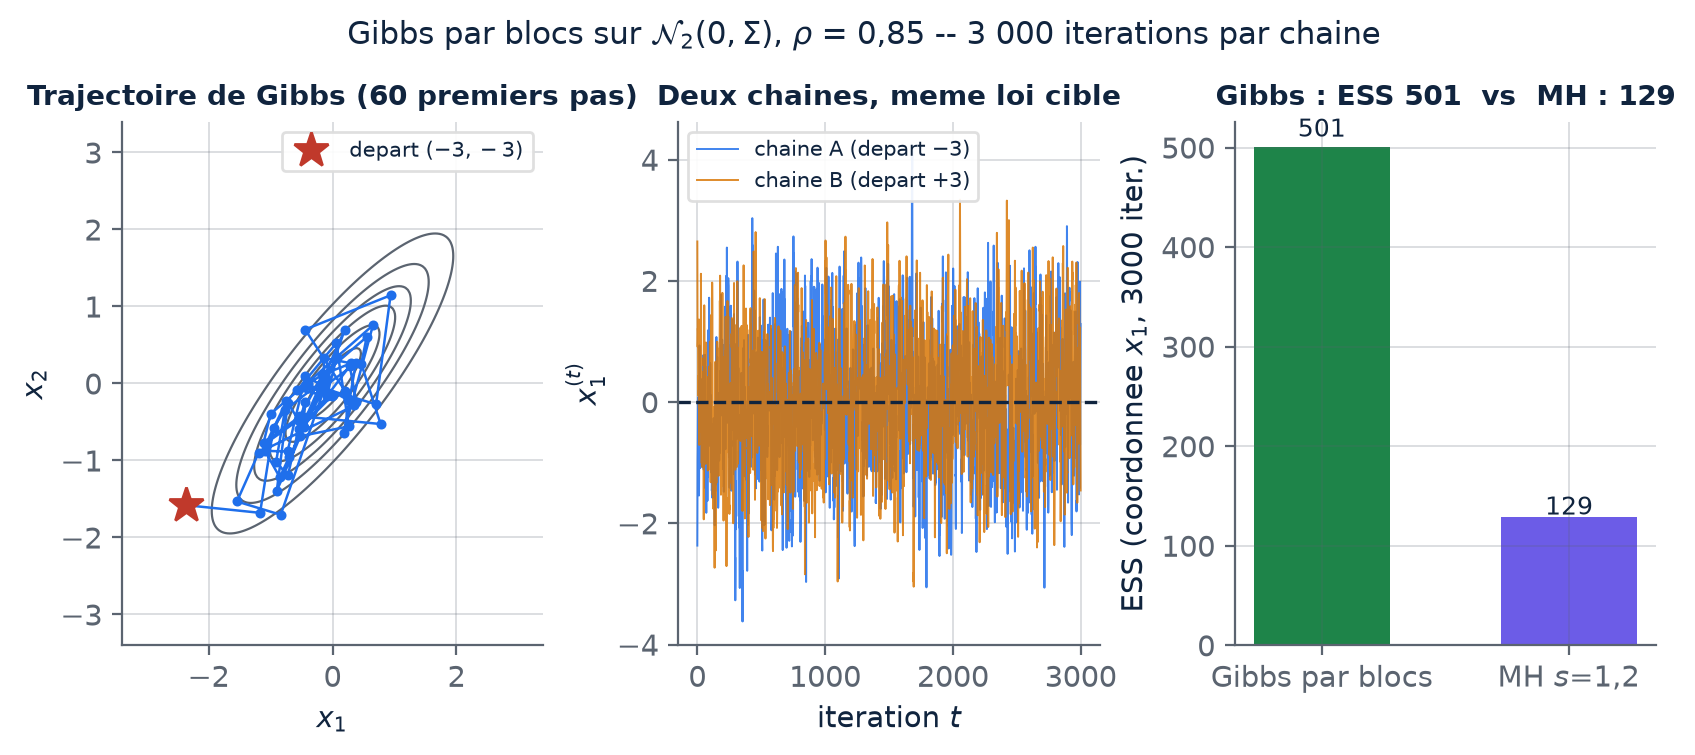
\includegraphics[width=.86\textwidth]{j07_gibbs_bivarie.png}
\end{center}
\end{frame}

% [split]
\begin{frame}{Gibbs exécuté : trajectoire et oubli de l'état initial}

\vspace{-2.5mm}
\begin{columns}[t]
\begin{column}{0.53\textwidth}
\begin{solbox}[Chiffres réels (script \file{src/fig\_ch5.py})]
\begin{itemize}
  \item Cible : $\N_2$ de corrélation 0,85 ; 3 000 itérations par chaîne.
  \item Trajectoire : de \emph{marches en escalier} (alternance
        verticale/horizontale) --- signature visuelle de Gibbs.
  \item Deux chaînes parties de $(-3,-3)$ et $(+3,+3)$ : la trace de $x_1$
        oublie le départ en quelques dizaines d'itérations.
  \item Moyenne obtenue : $-0{,}0272$ (vraie valeur 0) ; écart-type 1,0052
        (vraie valeur 1) ; corrélation 0,8465 (vraie valeur 0,85).
\end{itemize}
\end{solbox}
\end{column}
\begin{column}{0.45\textwidth}
\begin{qbox}[Question à se poser devant la figure]
Pourquoi la trajectoire de gauche ne se déplace-t-elle \textbf{jamais} en
diagonale ?
\vspace{1mm}
\\ \footnotesize Parce que le bloc mis à jour \emph{conditionne} sur la valeur
courante de l'autre bloc : on bouge un axe à la fois. Quand $\rho \to 1$, la cible
est un cigare très fin et Gibbs \emph{rame} le long du cigare.
\end{qbox}
\end{column}
\end{columns}
\end{frame}

% ---------------------------------------------------------------- 23
\begin{frame}{Gibbs : forces et faiblesses structurelles}
\footnotesize
\begin{columns}[t]
\begin{column}{0.49\textwidth}
\begin{kbox}[Forces]
\begin{itemize}
  \item \textbf{Aucun réglage} : pas de $s$, pas de $\varepsilon$, donc pas de
        phase d'adaptation.
  \item Tirages \textbf{exacts} à chaque bloc : acceptation 100 \%, et le
        posterior de chaque bloc est correctement échantillonné.
  \item Idéal pour les modèles à \textbf{structure conditionnelle simple} :
        régressions hiérarchiques, modèles à effets aléatoires, mélanges,
        modèles graphiques.
  \item Fournit naturellement un échantillonnage \emph{par blocs} : on ne
        simule que des lois de petite dimension.
\end{itemize}
\end{kbox}
\end{column}
\begin{column}{0.49\textwidth}
\begin{wbox}[Faiblesses]
\begin{itemize}
  \item Il faut connaître les \textbf{conditionnelles complètes} :
        \py{pm.Gibbs} n'existe pas pour un modèle écrit en langage PyMC --- on
        implémente Gibbs soi-même (conjugaison) ou on passe à NUTS.
  \item \textbf{Corrélations fortes} : le mouvement en escalier explore mal les
        directions obliques. Estimations numériques de référence : pour
        $\rho = 0{,}5$ l'ESS relatif reste élevé, mais pour $\rho \to 0{,}99$ il
        s'effondre ; c'est le reproche classique fait à Gibbs.
  \item \textbf{Multimodalité} : la chaîne reste dans un mode, et aucun
        réglage ne l'en fait sortir.
  \item Quand des composantes sont \textbf{très dépendantes} (centrée/non centrée),
        le choix de paramétrisation change tout (slide 30).
\end{itemize}
\end{wbox}
\end{column}
\end{columns}
\end{frame}

% ---------------------------------------------------------------- 24
\begin{frame}{De MH à HMC : et si la géométrie nous aidait ?}
% [rogna]
\footnotesize
\begin{columns}[t]
\begin{column}{0.5\textwidth}
\begin{ebox}[Le problème que MH et Gibbs ne résolvent pas]
\begin{itemize}
  \item Une marche aléatoire \textbf{découvre} la cible par tâtonnement
        ($\varepsilon$ : pas, direction tirée au hasard).
  \item Dans une direction étroite il faut de petits pas
        ($\varepsilon$), dans une direction large on avance trop lentement.
  \item Pour un modèle à 50 paramètres, la fraction de propositions acceptées
        s'effondre : c'est la \emph{malédiction de la dimension} des marcheurs
        aléatoires.
\end{itemize}
\end{ebox}
\end{column}
\begin{column}{0.48\textwidth}
\begin{kbox}[L'idée hamiltonienne]
Le \textbf{gradient} de $\log \tilde\pi$ indique où la densité augmente : au lieu
de proposer au hasard, on \emph{propose dans la bonne direction}, et suffisamment
loin.
\\[1mm]
On introduit un moment artificiel $p$ et l'on intègre une trajectoire physique
conservant l'\textbf{énergie}
\[
H(q,p) = \underbrace{-\log \tilde\pi(q)}_{U(q)}
\;+\; \underbrace{\tfrac12 p^{\!\top}p}_{K(p)}
\]
\centering\footnotesize $U$ : énergie potentielle ; $K$ : énergie cinétique.
Un mouvement conservatif visite la cible \emph{sans} errer : les propositions
lointaines deviennent très souvent acceptées.
\end{kbox}
\end{column}
\end{columns}
\vspace{1mm}
\begin{tcolorbox}[colback=byCyan!8,colframe=byCyan,arc=2mm,width=.96\textwidth]
\small\centering
\textbf{Coût du progrès :} HMC demande le gradient. En pratique, et c'est le cas
dans PyMC, ce gradient est obtenu par \textbf{différenciation automatique} du
log-posterior --- aucune dérivée n'est écrite à la main.
\end{tcolorbox}
\end{frame}

% ---------------------------------------------------------------- 25
\begin{frame}{Dynamique hamiltonienne expliquée (et vérifiée à l'écran)}
\footnotesize
\begin{columns}[t]
\begin{column}{0.52\textwidth}
\begin{ebox}[Les deux équations]
\[
\frac{\mathrm{d}q}{\mathrm{d}t} = \frac{\partial H}{\partial p} = p,
\qquad
\frac{\mathrm{d}p}{\mathrm{d}t} = -\frac{\partial H}{\partial q}
= \nabla \log \tilde\pi(q).
\]
L'état parcourt une courbe de \textbf{niveau d'énergie constant} : il glisse dans
les vallées du log-posterior. Deux propriétés sont préservées exactement par la
dynamique continue : le volume (théorème de Liouville) et l'énergie.
\end{ebox}
\begin{kbox}[La distribution cible en sort gratuitement]
Si $p \sim \N(0, I)$ et si l'on part de $q$ quelconque, alors $q$ \emph{après} la
trajectoire est distribué selon $\pi$ : le moment joue le rôle d'une variable
auxiliaire jetable. C'est une \textbf{augmentation} de la cible, exactement comme
au chapitre 2 pour les variables latentes.
\end{kbox}
\end{column}
\begin{column}{0.46\textwidth}
\begin{center}
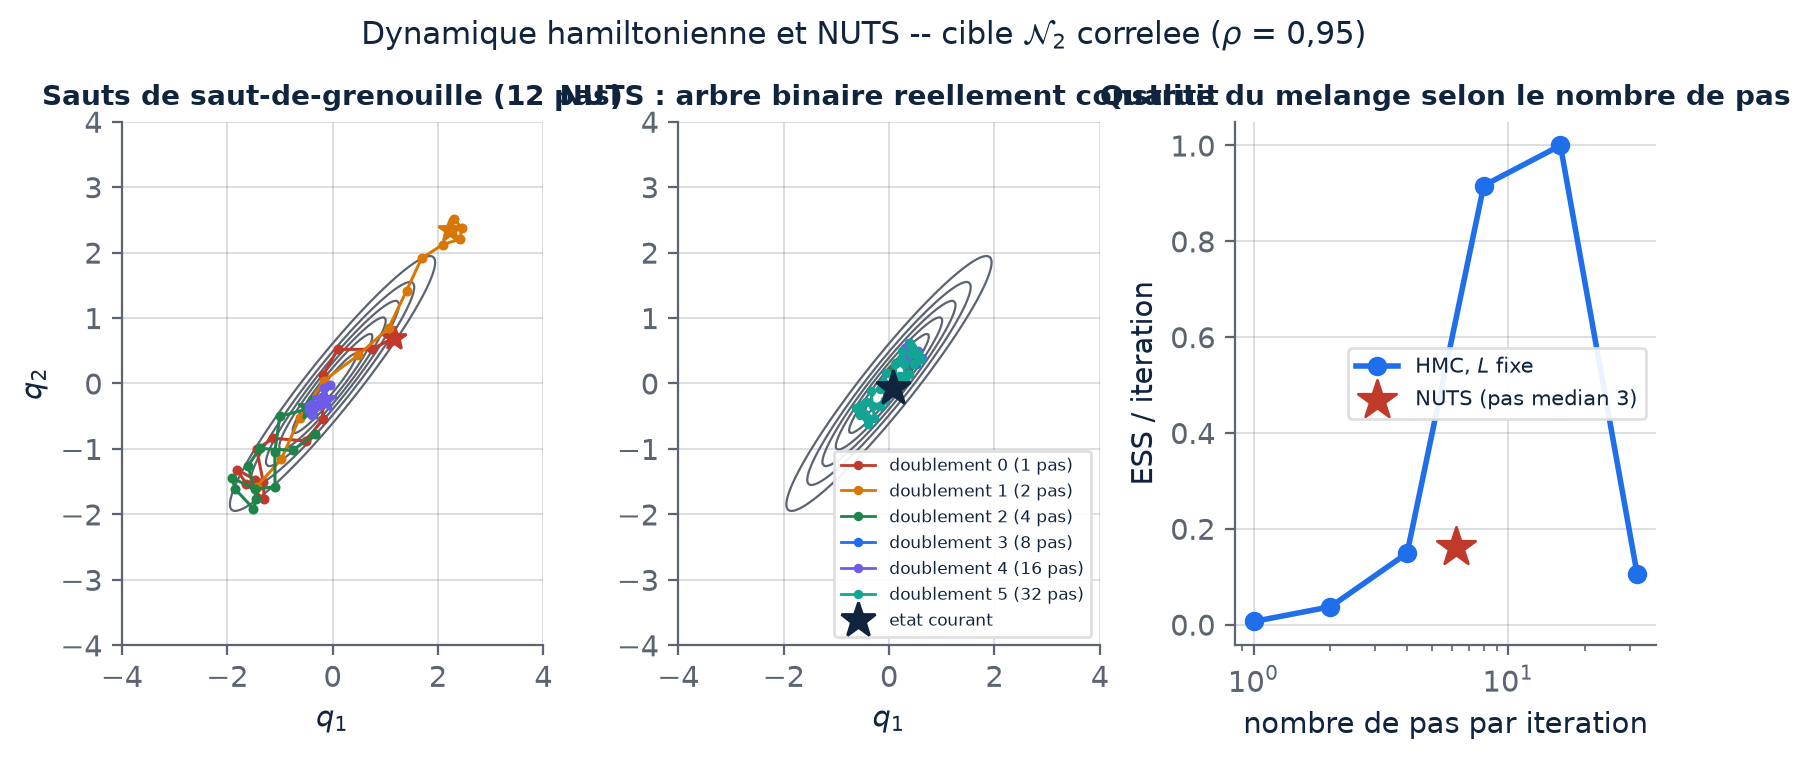
\includegraphics[width=\textwidth]{j08_hmc_nuts.png}
\end{center}
\vspace{-2mm}
\centering\footnotesize
Sauts de saut-de-grenouille (12 pas, $\varepsilon = 0{,}30$) sur une cible
$\N_2$ de corrélation 0,95 ; à droite, le doublement d'arbre de NUTS.
\end{column}
\end{columns}
\end{frame}

% ---------------------------------------------------------------- 26
\begin{frame}[fragile]{Saut-de-grenouille : l'intégrateur en dix lignes}
\footnotesize
\begin{columns}[t]
\begin{column}{0.53\textwidth}
\begin{codebox}[leapfrog.py --- intégrateur symplectique, exécuté]
\begin{lstlisting}
def leapfrog(q, p, eps, L, logp_grad):
    # p <- p + (eps/2) * grad log pi(q)
    qn, pn = q.copy(), p.copy()
    _, g = logp_grad(qn)
    pn += 0.5 * eps * g
    for _ in range(L - 1):        # L-1 pas complets
        qn += eps * pn
        _, g = logp_grad(qn)
        pn += eps * g
    qn += eps * pn                # dernier pas complet
    _, g = logp_grad(qn)
    pn += 0.5 * eps * g           # demi-pas final
    return qn, pn
\end{lstlisting}
\end{codebox}
\end{column}
\begin{column}{0.45\textwidth}
\begin{ebox}[Puis on corrige par Metropolis]
\begin{enumerate}
  \item tirer $p \sim \N(0, I)$ ;
  \item calculer $H_0 = -\log\tilde\pi(q) + \tfrac12 p^{\!\top}p$ ;
  \item intégrer $L$ pas : $(q,p) \to (q^\star, p^\star)$ ;
  \item calculer $H_1$ au nouveau point ;
  \item accepter avec probabilité $\min\!\big(1, e^{H_0 - H_1}\big)$.
\end{enumerate}
\end{ebox}
\begin{kbox}[Ce qu'il faut retenir du code]
\small
Le \emph{demi-pas} au début et à la fin n'est pas une coquetterie : c'est ce qui
rend l'intégrateur \textbf{symplectique} et \textbf{réversible}, donc valide pour
la correction de Metropolis. Écrire les deux demi-pas entiers casse la
réversibilité et biaise l'échantillon.
\end{kbox}
\end{column}
\end{columns}
\end{frame}

% ---------------------------------------------------------------- 27
\begin{frame}{HMC exécuté : les chiffres, et le prix du pas $L$}
\footnotesize
\begin{columns}[t]
\begin{column}{0.49\textwidth}
\begin{solbox}[HMC maison, 3 000 itérations, $\varepsilon = 0{,}30$, $L = 10$]
\begin{tabular}{@{}ll@{}}
\toprule
quantité & mesure \\
\midrule
acceptation & \textbf{85,2 \%} \\
ESS sur $x_1$ & \textbf{3 000 / 3 000} \\
erreur d'énergie $|\Delta H|$ & $< 0{,}01$ \\
évaluations de gradient & 10 par tirage \\
ESS par évaluation & 0,100 \\
\bottomrule
\end{tabular}
\vspace{1.5mm}
\\ Le même tirage par MH réglé donne ESS = 128,8 sur 3 000 : HMC obtient ici
\textbf{23 fois plus} d'échantillons utiles, au prix du gradient.
\end{solbox}
\begin{kbox}[Le réglage de $L$, mesuré]
\begin{tabular}{@{}lrrrrrr@{}}
\toprule
$L$ & 1 & 2 & 4 & 8 & 16 & 32 \\
ESS & 13 & 75 & 298 & 1 833 & 2 000 & 213 \\
\bottomrule
\end{tabular}
\vspace{1mm}
\\ Trop court, la trajectoire n'avance pas (ESS 13) ; trop long, elle revient sur
ses pas (ESS retombe à 213). Il faut donc régler $L$ --- sauf avec NUTS.
\end{kbox}
\end{column}
\begin{column}{0.49\textwidth}
\begin{qbox}[Pourquoi ne pas toujours prendre $L$ énorme ?]
\begin{itemize}
  \item Chaque pas coûte une évaluation du gradient : le budget est
        proportionnel à $L$.
  \item Au-delà d'un demi-tour de la cible, la trajectoire \textbf{rebrousse
        chemin} : on paie des pas qui ramènent près du départ.
  \item Mesure : $L = 16$ donne ESS = 2 000 pour 32 000 évaluations ; $L = 8$
        donne ESS = 1 833 pour 16 000 évaluations --- \emph{deux fois} moins
        cher pour un résultat quasi identique.
\end{itemize}
\end{qbox}
\end{column}
\end{columns}
\end{frame}

% ---------------------------------------------------------------- 28
\begin{frame}{NUTS : laisser la trajectoire décider}
\footnotesize
\begin{columns}[t]
\begin{column}{0.53\textwidth}
\begin{ebox}[No-U-Turn Sampler]
L'arbre est construit par \textbf{doublement} :
\begin{enumerate}
  \item partir de l'état courant, choisir au hasard un sens (avant/arrière) ;
  \item intégrer $2^0, 2^1, 2^2, \dots$ pas, garder un candidat tiré uniformément
        parmi les états retenus ;
  \item s'arrêter au \emph{U-turn} : $\langle q_+ - q_-, p_\pm \rangle < 0$.
\end{enumerate}
\end{ebox}
\begin{kbox}[Mesures sur la cible corrélée (corrélation 0,95), pas de 0,30]
\begin{tabular}{@{}ll@{}}
\toprule
pas par itération & médiane \textbf{3}, moyenne 6,2, maximum 15 \\
divergences & \textbf{0} sur 800 itérations \\
ESS sur $x_1$ & 129,9 sur 800, soit 0,162 par tirage \\
\bottomrule
\end{tabular}
\vspace{1mm}
\\ Sur cette cible 2D lisse, un $L$ bien réglé reste meilleur : NUTS paye le coût
d'explorer plusieurs longueurs. Son intérêt premier est de \textbf{supprimer le
réglage} et de rester efficace sur des cibles à courbure variable.
\end{kbox}
\end{column}
\begin{column}{0.48\textwidth}
\begin{qbox}[Et si l'on n'a pas le gradient ?]
Sur un modèle à \textbf{variables latentes discrètes} (allocation de mélange,
chaîne de Markov cachée), le gradient n'existe pas : on revient à Gibbs ou au
Metropolis à l'intérieur de Gibbs. NUTS n'est pas universel --- il exige un
log-posterior \textbf{différentiable}.
\end{qbox}
\end{column}
\end{columns}
\end{frame}

% ---------------------------------------------------------------- 29
\begin{frame}{Divergences : le diagnostic qui sauve une analyse}
\footnotesize
\begin{columns}[t]
\begin{column}{0.5\textwidth}
\begin{wbox}[Ce qu'est une divergence]
Sur une trajectoire, l'intégrateur doit conserver l'énergie : $|\Delta H|$
reste proche de 0. Une \textbf{divergence} est un pas où
$|\Delta H|$ explose (seuil usuel : $10^2$ à $10^3$) : la trajectoire est partie
dans une zone où la courbure est trop forte pour le pas $\varepsilon$.
\\[1mm]
Conséquence : le point est rejeté \emph{en silence} et l'on reste sur place.
La chaîne paraît acceptée correctement, mais elle \textbf{rate une région} du
posterior.
\end{wbox}
\begin{kbox}[Ce qu'il faut faire]
\begin{itemize}
  \item Elles sont \textbf{visibles} : \py{idata.sample_stats.diverging}.
  \item \textbf{Jamais} d'analyse sans avoir vérifié qu'il n'y en a pas.
  \item Remèdes, dans l'ordre : augmenter le \py{target\_accept}
        ($0{,}9 \to 0{,}99$), reparamétrer, simplifier le modèle.
\end{itemize}
\end{kbox}
\end{column}
\begin{column}{0.48\textwidth}
\begin{solbox}[Mesures du script --- funnel à 9 effets]
Toutes deux avec $\varepsilon = 0{,}25$, $L = 10$, 1 500 itérations :
\begin{tabular}{@{}lll@{}}
\toprule
& \textbf{centrée} & \textbf{non centrée} \\
\midrule
divergences & \textbf{17} (1,13 \%) & \textbf{0} \\
$|\Delta H|$ maximal & 812,5 & 0,10 \\
acceptation & 78,8 \% & 98,6 \% \\
ESS de $y$ & 33,8 & \textbf{286,7} \\
ESS / $N$ & 0,023 & \textbf{0,191} \\
\bottomrule
\end{tabular}
\vspace{1mm}
\\ Le même modèle, le même échantillonneur, le même budget : seule la
paramétrisation change, et l'efficacité est multipliée par 8.
\end{solbox}
\end{column}
\end{columns}
\end{frame}

% ---------------------------------------------------------------- 30
\begin{frame}{Reparamétrisation centrée contre non centrée : le funnel}
\footnotesize
\begin{center}
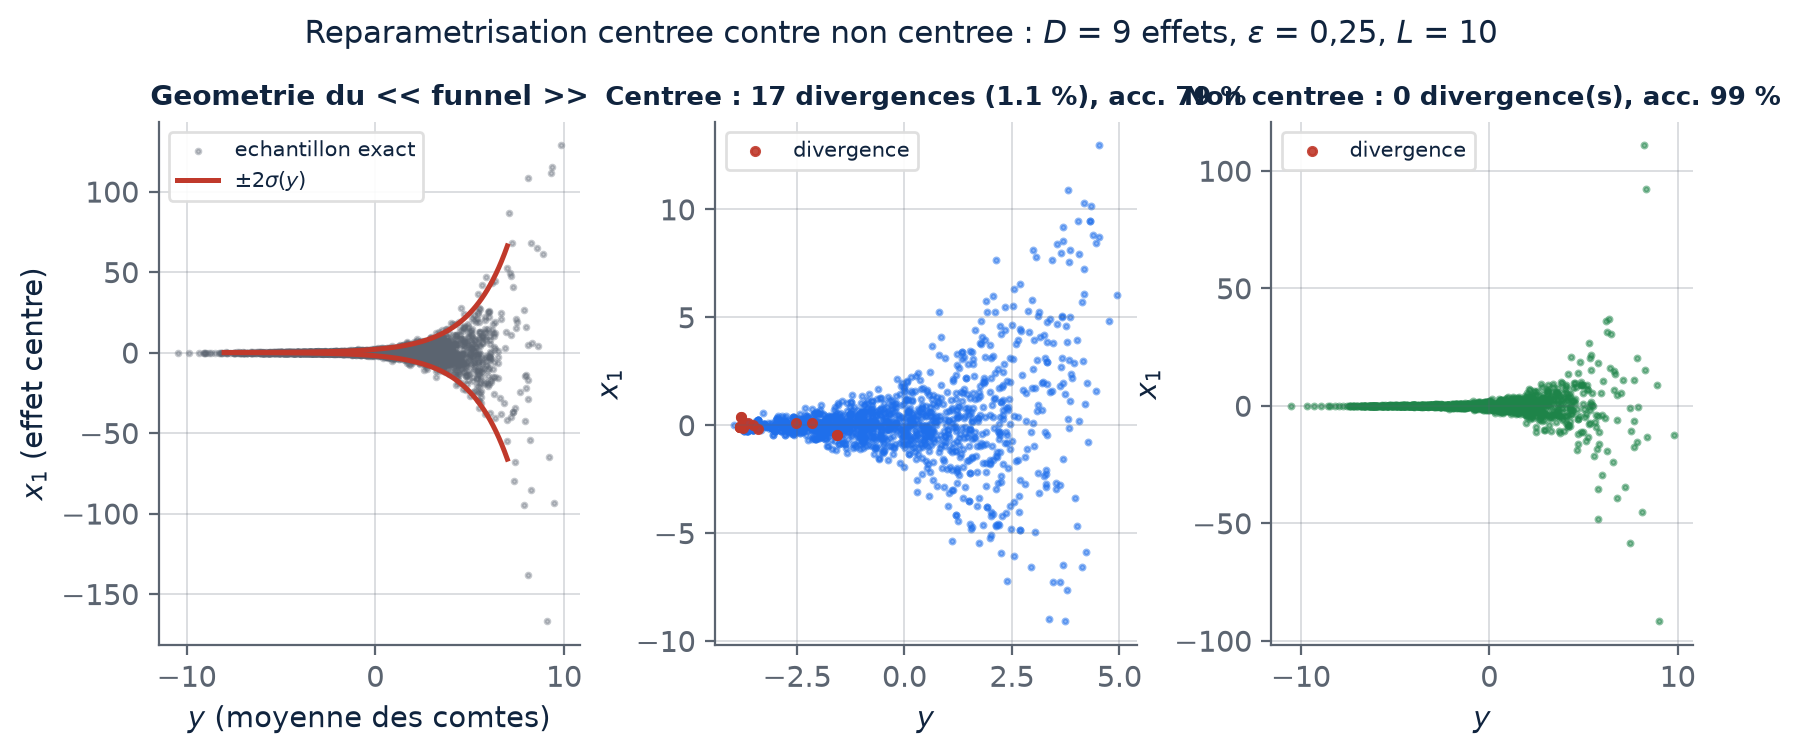
\includegraphics[width=.68\textwidth]{j09_funnel_centree.png}
\end{center}
\vspace{-3mm}
\begin{columns}[t]
\begin{column}{0.49\textwidth}
\begin{ebox}[Deux écritures du même modèle]
\textbf{Centrée :} $y \sim \N(0,3)$, \; $x_i \given y \sim \N\!\big(0, e^{y/2}\big)$ :
l'échelle des $x_i$ \emph{change avec} $y$, la densité dessine un entonnoir.
\\[1mm]
\textbf{Non centrée :} $y \sim \N(0,3)$, \; $z_i \sim \N(0,1)$,
\; $x_i = z_i\,e^{y/2}$ : la courbure vue par l'échantillonneur est constante.
\end{ebox}
\end{column}
\begin{column}{0.49\textwidth}
\begin{qbox}[Question de TP]
Dans un modèle hiérarchique $y_{ij} = a_j + b x_{ij} + \varepsilon$, quand
écrire $a_j \sim \N(\mu_a, \sigma_a)$ et quand
$a_j = \mu_a + \sigma_a z_j$, $z_j \sim \N(0,1)$ ?
\vspace{1mm}
\\ \footnotesize Règle : \textbf{peu} d'observations par groupe $\Rightarrow$
non centré ; \textbf{beaucoup} par groupe $\Rightarrow$ centré. Le mini-projet
tranche expérimentalement (section 5.5), et les mesures de la slide précédente
montrent l'enjeu : ESS multiplié par 8, divergences ramenées à 0.
\end{qbox}
\end{column}
\end{columns}
\end{frame}

% ---------------------------------------------------------------- 31
% [suite]
\begin{frame}{Choisir son échantillonneur : arbre de décision}
% [rogna]
\footnotesize
\begin{center}
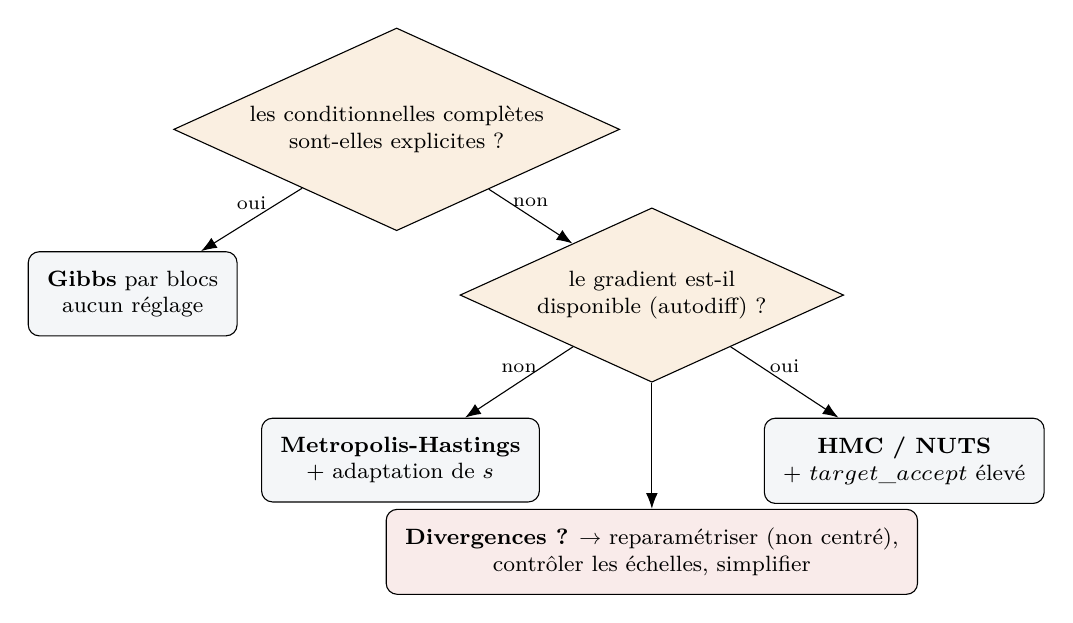
\begin{tikzpicture}[every node/.style={font=\footnotesize},node distance=4mm,
  box/.style={draw,rounded corners,fill=byLight,inner sep=2.4mm,align=center},
  dec/.style={draw,diamond,aspect=2.2,fill=byOrange!12,inner sep=1mm,align=center}]
\node[dec] (q1) {les conditionnelles complètes\\sont-elles explicites ?};
\node[box,below left=9mm and 6mm of q1] (g) {\textbf{Gibbs} par blocs\\aucun réglage};
\node[dec,below right=9mm and 6mm of q1] (q2) {le gradient est-il\\disponible (autodiff) ?};
\node[box,below left=10mm and 2mm of q2] (mh) {\textbf{Metropolis-Hastings}\\+ adaptation de $s$};
\node[box,below right=10mm and 2mm of q2] (h) {\textbf{HMC / NUTS}\\+ $target\_accept$ élevé};
\node[box,below=16mm of q2,fill=byRed!10] (rep) {\textbf{Divergences ?} $\rightarrow$ reparamétriser (non centré),\\contrôler les échelles, simplifier};
\draw[-{Latex[length=2mm]}] (q1) -- node[above,font=\scriptsize]{oui} (g);
\draw[-{Latex[length=2mm]}] (q1) -- node[above,font=\scriptsize]{non} (q2);
\draw[-{Latex[length=2mm]}] (q2) -- node[above,font=\scriptsize]{non} (mh);
\draw[-{Latex[length=2mm]}] (q2) -- node[above,font=\scriptsize]{oui} (h);
\draw[-{Latex[length=2mm]}] (q2) -- (rep);
\end{tikzpicture}
\end{center}
\vspace{-3mm}
\end{frame}

% [suite]
\begin{frame}{Choisir son échantillonneur : arbre de décision (suite)}
\begin{columns}[t]
\begin{column}{0.49\textwidth}
\begin{abox}[Le réflexe industriel : NUTS par défaut]
Dans PyMC, \py{pm.sample()} appelle NUTS avec adaptation du pas. On ne choisit
donc pas son échantillonneur dans 90 \% des cas : on choisit sa
\textbf{paramétrisation} et son \py{target\_accept}. C'est là que passe
l'essentiel du temps de débogage.
\end{abox}
\end{column}
\begin{column}{0.49\textwidth}
\begin{wbox}[Trois signaux d'alerte]
\nok{} des \textbf{divergences}, même 2 ou 3 sur 4 000 tirages :\;
elles indiquent une zone non explorée.\\
\nok{} un $\hat R > 1{,}01$ sur un paramètre : \; ne tirez aucune conclusion.\\
\nok{} un ESS \textbf{inférieur à 100} pour un paramètre d'intérêt : \; l'intervalle
de crédibilité sera instable d'une exécution à l'autre.
\end{wbox}
\end{column}
\end{columns}
\end{frame}

% ---------------------------------------------------------------- 32
\begin{frame}{Exercice encadré : régler une proposition comme un pro}
\footnotesize
\begin{abox}[Consigne (15 min, binôme, machine)]
Reprendre le MH maison de la slide 15 sur la cible Beta$(2{,}5\,;\,7)$ et :
\begin{enumerate}
  \item écrire une boucle qui teste $s \in \{0{,}01 ; 0{,}02 ; 0{,}05 ; 0{,}1 ;
        0{,}2 ; 0{,}35 ; 0{,}6 ; 1{,}0 ; 1{,}8 ; 3{,}0 ; 6{,}0\}$ sur 20 000 itérations ;
  \item tracer l'ESS en fonction de $s$ et marquer le maximum ;
  \item vérifier que l'ESS maximal est atteint pour $s \approx 0{,}35$ et que
        l'acceptation y vaut environ 41 \% ;
  \item refaire l'expérience avec une proposition \emph{uniforme}
        $\theta^\star \sim \mathrm{U}(\theta - s, \theta + s)$ et comparer les ESS ;
  \item conclure : quelle famille de propositions choisir et pourquoi.
\end{enumerate}
\end{abox}
\vspace{1mm}
\begin{columns}[t]
\begin{column}{0.49\textwidth}
\begin{solbox}[Résultats de référence (attendus)]
$s$ optimal mesuré : \textbf{0,35}, ESS = \textbf{4 070} sur 20 000
(soit 0,204 par tirage), acceptation 41,4 \%. Le pire cas mesuré est
$s = 0{,}01$ : ESS = \textbf{21}, acceptation 97,6 \%.
\end{solbox}
\end{column}
\begin{column}{0.49\textwidth}
\begin{kbox}[Ce que l'exercice fait comprendre]
Un pas trop grand \emph{et} un pas trop petit sont deux échecs symétriques. Le
critère de jugement n'est jamais le taux d'acceptation seul : c'est l'ESS
(lui-m\^eme estimé sur une chaîne assez longue pour être fiable).
\end{kbox}
\end{column}
\end{columns}
\end{frame}

% ---------------------------------------------------------------- 33
\begin{frame}{Synthèse 5.3 --- Gibbs, HMC et NUTS}
\footnotesize
\begin{columns}[t]
\begin{column}{0.52\textwidth}
\begin{tcolorbox}[enhanced,colback=byPurple!7,colframe=byPurple,arc=2mm,
   title={\bfseries\color{white}\faLightbulb\ Synthèse},colbacktitle=byPurple,
   attach boxed title to top left={xshift=3mm,yshift=-2mm},
   boxed title style={arc=1mm,boxrule=0pt}]
\begin{itemize}
  \item \textbf{Gibbs} : exact, sans réglage, imbattable si les conditionnelles
        sont closes --- ESS 0,167 par tirage contre 0,043 pour MH sur la même cible.
  \item \textbf{HMC} : le gradient transforme la marche aléatoire en trajectoire
        physique (acceptation 85 \%, ESS = 3 000 sur 3 000 tirages, mais
        10 évaluations de gradient par tirage).
  \item Le réglage de $L$ est un vrai piège (ESS : 13 pour $L = 1$, 2 000 pour
        $L = 16$, 213 pour $L = 32$) ; \textbf{NUTS} le supprime par doublement
        d'arbre (médiane 3 pas ici).
  \item \textbf{Divergences} et \textbf{reparamétrisation} : sur le funnel,
        17 divergences et ESS/\,$N$ = 0,023 en centré contre \textbf{0 divergence
        et ESS/\,$N$ = 0,191} en non centré --- à modèle identique.
\end{itemize}
\end{tcolorbox}
\end{column}
\begin{column}{0.46\textwidth}
\begin{abox}[À faire avant la séance 6]
\begin{itemize}
  \item Reproduire les trois échantillonneurs maison
        (\file{src/fig\_ch5*.py}) et vérifier les ordres de grandeur du tableau.
  \item Refaire le funnel avec $D = 1$ (un seul effet) : les divergences
        disparaissent-elles ? Pourquoi ?
  \item Sur une cible $\N_2$ de corrélation 0,99, comparer Gibbs et HMC :
        qui gagne, et de combien ?
  \item Lire \py{az.plot_rank} sur les chaînes HMC produites.
\end{itemize}
\end{abox}
\begin{tcolorbox}[colback=byCyan!8,colframe=byCyan,arc=2mm]
\small\textbf{Fil rouge :} tout échantillonneur est jugé sur \emph{trois}
choses --- la justesse (invariance), l'efficacité (ESS), la couverture
(aucune zone perdue : divergences, chaînes multiples).
\end{tcolorbox}
\end{column}
\end{columns}
\end{frame}

% ---------------------------------------------------------------- 34
% [suite]
\begin{frame}{Diagnostics : la liste de contrôle à passer en revue}
% [rogna]
\footnotesize
\begin{center}
\footnotesize
\begin{tabular}{@{}p{3.0cm}p{3.4cm}p{3.0cm}p{4.2cm}@{}}
\toprule
\textbf{Diagnostic} & \textbf{Ce qu'il détecte} & \textbf{Seuil d'alerte} & \textbf{Commande PyMC / ArviZ} \\
\midrule
Trace plot & non-stationnarité, sauts, tendance & visuelle & \py{az.plot_trace(idata)} \\[1.5mm]
Rank plot & modes non visités, chaînes divergentes & non uniforme & \py{az.plot_rank(idata)} \\[1.5mm]
$\hat R$ (R-hat) & désaccord entre et dans les chaînes & $> 1{,}01$ & \py{az.rhat(idata)} \\[1.5mm]
ESS (bulk / tail) & autocorrélation, queues mal explorées & $< 400$ \; (\;proche de 100 : alerte) & \py{az.ess(idata)} \\[1.5mm]
Divergences & géométrie pathologique & $> 0$ & \py{idata.sample\_stats.diverging} \\[1.5mm]
MCSE & erreur de simulation sur la moyenne & comparer à l'effet cherché & \py{az.mcse(idata)} \\[1.5mm]
PPC & modèle inadéquat (pas l'échantillonneur) & couverture $\ne$ 94 \% & \py{az.plot\_ppc(idata)} \\
\bottomrule
\end{tabular}
\end{center}
\vspace{1mm}
\end{frame}

% [suite]
\begin{frame}{Diagnostics : la liste de contrôle à passer en revue (suite)}
\begin{columns}[t]
\begin{column}{0.49\textwidth}
\begin{kbox}[La règle des quatre questions]
\begin{enumerate}
  \item La chaîne a-t-elle \textbf{oublié} son départ ? (trace, burn-in)
  \item Les chaînes \textbf{racontent-elles la même histoire} ? ($\hat R$, rank)
  \item Y a-t-il assez de tirages \textbf{utiles} ? (ESS, MCSE)
  \item Le modèle est-il \textbf{adéquat} ? (PPC) --- question distincte des trois
        premières : un échantillonneur parfait peut valider un mauvais modèle.
\end{enumerate}
\end{kbox}
\end{column}
\begin{column}{0.49\textwidth}
\begin{wbox}[Deux confusions à ne plus faire]
\nok{} Confondre \textbf{convergence de la chaîne} et \textbf{qualité du modèle} :
les diagnostics ne jugent que le premier point.
\\[1mm]
\nok{} Croire qu'un $\hat R$ parfait suffit : deux chaînes peuvent être d'accord
sur \emph{un} mode alors que la cible en compte deux.
\end{wbox}
\end{column}
\end{columns}
\end{frame}

% ---------------------------------------------------------------- 35
\begin{frame}{Anatomie d'un rapport de diagnostics (résultats PyMC réels)}
\begin{center}
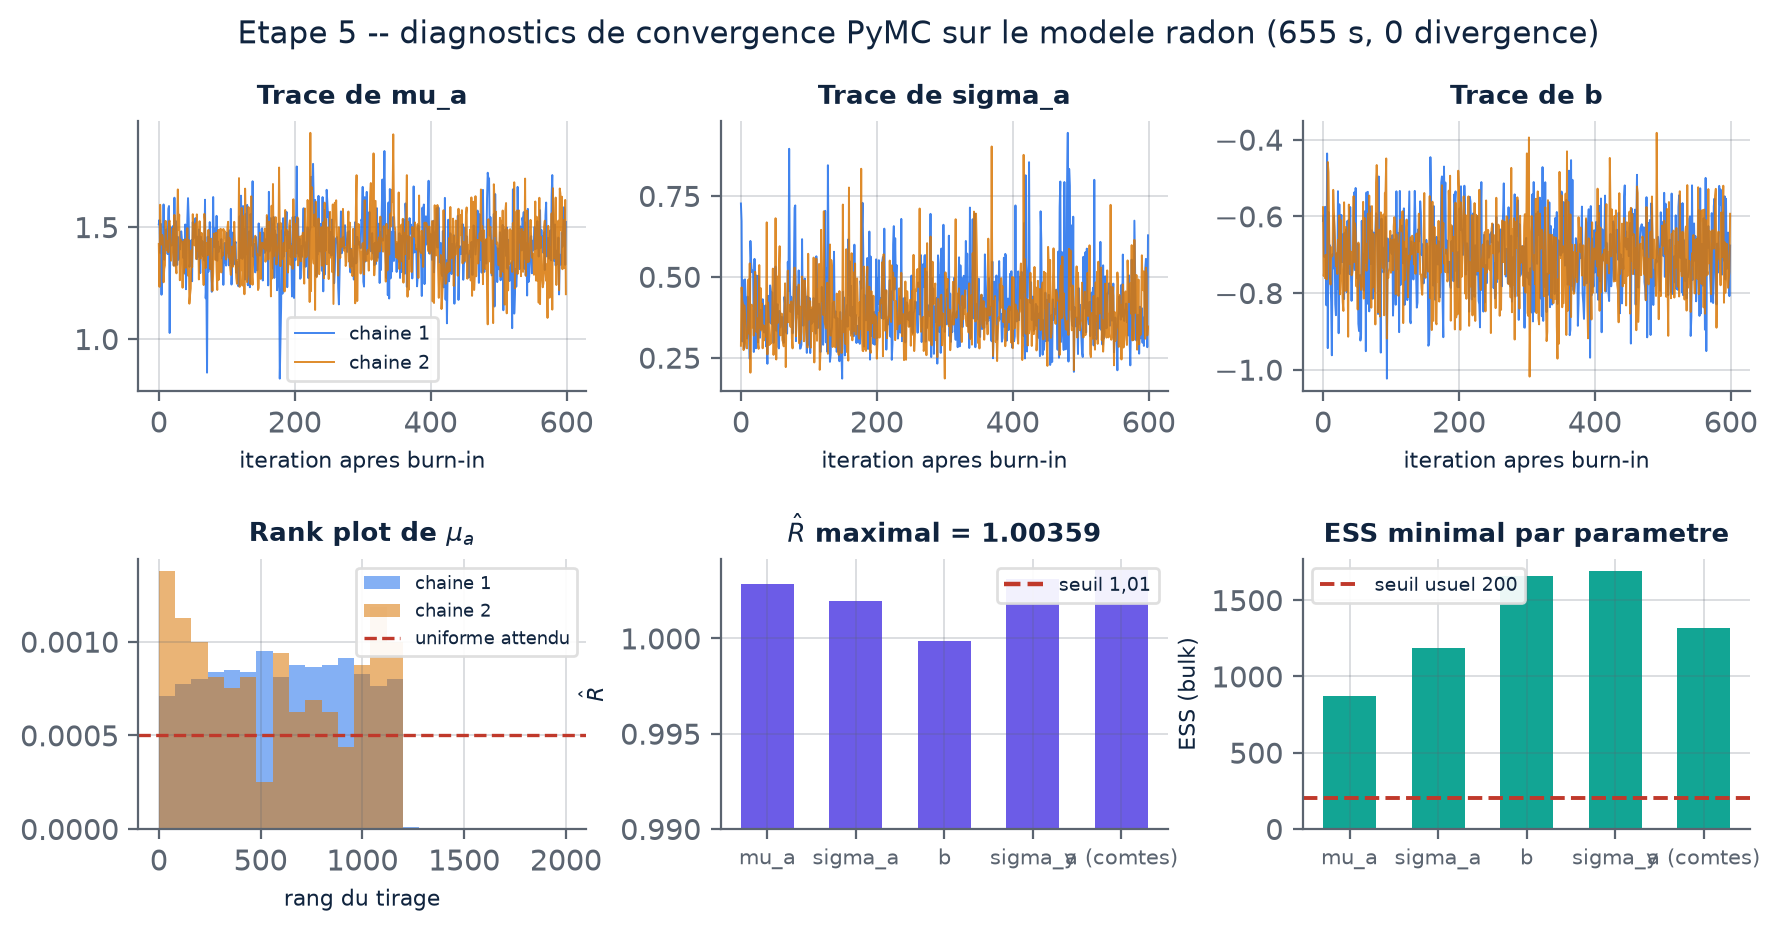
\includegraphics[width=0.90\textwidth]{j10_pymc_diagnostics.png}
\end{center}
\vspace{-1.5mm}
\centering\footnotesize
Modèle hiérarchique radon (section 5.5), 2 chaînes $\times$ 1 000 tirages après
1 000 de chauffe, \py{target\_accept=0.9}, \py{cores=1} :
$\hat R_{\max} = $ 1,00311 \;; \; ESS minimal = 872 \;; \;
divergences = 0 \;; \; temps d'échantillonnage 655~s.
\end{frame}

% ---------------------------------------------------------------- 36
\begin{frame}{Le trace plot : cinq pathologies à reconnaître}
% [rogna]
\small
\begin{columns}[t]
\begin{column}{0.53\textwidth}
\begin{ebox}[Ce qu'on regarde]
\begin{enumerate}
  \item Deux chaînes qui \textbf{ne se recouvrent pas} : \;
        $\hat R$ explose, rien n'est stationnaire.
  \item Une \textbf{tendance} qui persiste après le burn-in : \;
        la chauffe était trop courte (ou la chaîne se déplace lentement).
  \item De \textbf{longs paliers} : \;
        proposition trop large --- ESS effondré (mesuré : ESS = 130 à $s = 6$).
  \item Une trace \textbf{trop lisse}, sans bruit : \;
        proposition trop étroite --- ESS = 46 à $s = 0{,}02$.
  \item Une chaîne \textbf{plate} à une valeur : \;
        le paramètre n'est pas identifié par les données, ou le prior est écrasant.
\end{enumerate}
\end{ebox}
\end{column}
\begin{column}{0.45\textwidth}
\begin{kbox}[Comment le lire efficacement]
\begin{itemize}
  \item Toujours \textbf{superposer} les chaînes d'une même couleur.
  \item Ne pas juger sur 100 itérations : afficher au moins 500 à 1 000 tirages
        par chaîne.
  \item La trace est un diagnostic \emph{qualitatif} : elle \emph{complète}
        $\hat R$ et l'ESS, elle ne les remplace pas.
  \item Sur 200 paramètres \emph{on ne regarde pas} les 200 traces : on regarde
        les 5 paramètres d'intérêt et les cas signalés par $\hat R$.
\end{itemize}
\end{kbox}
\begin{tcolorbox}[colback=byCyan!8,colframe=byCyan,arc=2mm]
\small\textbf{Réflexe :} une trace saine ressemble à du \emph{bruit autour d'un
niveau stable}, sans structure visible.
\end{tcolorbox}
\end{column}
\end{columns}
\end{frame}

% ---------------------------------------------------------------- 37
% [suite]
\begin{frame}{Rank plot : voir ce que le trace plot cache}
\begin{columns}[t]
\begin{column}{0.52\textwidth}
\begin{ebox}[Construction]
Pour un paramètre et ses $K$ chaînes :
\begin{enumerate}
  \item empiler tous les tirages de toutes les chaînes ;
  \item remplacer chaque tirage par son \textbf{rang} dans cet ensemble ;
  \item histogrammer les rangs \emph{séparément par chaîne}.
\end{enumerate}
Si les chaînes ont convergé, chaque histogramme est \textbf{uniforme} sur
$[0, KN]$ : aucune chaîne ne concentre les grandes ou les petites valeurs.
\end{ebox}
\end{column}
\begin{column}{0.46\textwidth}
\begin{kbox}[Les deux motifs pathologiques]
\begin{itemize}
  \item \textbf{Rangs groupés à une extrémité} pour une chaîne : elle est restée
        dans une région de faible densité $\Rightarrow$ mode non visité,
        initialisation mal placée.
  \item \textbf{Forme en U} (les extrêmes sur-représentés) : les queues sont mal
        échantillonnées $\Rightarrow$ intervalles de crédibilité trop étroits :
        exactement le risque qu'on cherche à éviter.
\end{itemize}
\end{kbox}
\end{column}
\end{columns}
\end{frame}

% [suite]
\begin{frame}{Rank plot : voir ce que le trace plot cache (suite)}
\begin{solbox}[Sur nos chaînes radon]
Les rangs des deux chaînes sont uniformes : le trace plot \emph{et} le rank plot
concordent. Quand les deux se contredisent, c'est le rank plot qui a raison sur
la question des modes multiples.
\end{solbox}

\end{frame}

% ---------------------------------------------------------------- 38
\begin{frame}{R-hat : le désaccord entre et dans les chaînes}
% [rogna]
\footnotesize
\begin{columns}[t]
\begin{column}{0.53\textwidth}
\begin{ebox}[Définition opérationnelle]
Avec $m$ chaînes de longueur $n$ :
\[
\hat R = \sqrt{\frac{\hat V}{W}}, \qquad
W = \text{variance intra-chaîne},
\]
et $\hat V$ combine $W$ et la variance \textbf{entre} les moyennes de chaînes.
\\[1mm]
Intuition : si les chaînes ont oublié leur point de départ, la variabilité
\emph{entre} chaînes est du même ordre que la variabilité \emph{dans} une chaîne,
donc $\hat R \to 1$ par le haut.
\end{ebox}
\begin{kbox}[Le seuil de 1,01, et pourquoi il est si strict]
Un $\hat R$ de 1,1 peut cacher des intervalles de crédibilité sous-estimés de
30 \% : l'échelle est en $\sqrt{\cdot}$, donc 1,01 en $\hat R$ signifie déjà un
écart de 2 \% sur les variances. En 2026 on rapporte le \emph{maximum} de
$\hat R$ sur \emph{tous} les paramètres, y compris les effets de groupe.
\end{kbox}
\end{column}
\begin{column}{0.45\textwidth}
\begin{solbox}[Mesures de la section 5.5 (modèle radon)]
\footnotesize\begin{tabular}{@{}p{4.3cm}p{1.6cm}@{}}
\toprule
paramètre & $\hat R$ \\
\midrule
maximum sur $\mu_a$, $\sigma_a$, $b$, $\sigma_y$ & 1,00311 \\
maximum sur les 12 intercepts $a_j$ & 1,00359 \\
\midrule
$\hat R_{\max}$ global & \textbf{1,00311} \\
\bottomrule
\end{tabular}
\vspace{1.5mm}
\\ Le seuil de 1,01 est respecté partout : on peut lire les intervalles de crédibilité.
\end{solbox}
\begin{wbox}[Et si $\hat R$ vaut 1,00 avec 50 tirages ?]
Un $\hat R$ parfait ne prouve rien si l'ESS vaut 3. \;\textbf{Toujours} lire
$\hat R$ \emph{et} ESS ensemble : ce sont deux pathologies différentes.
\end{wbox}
\end{column}
\end{columns}
\end{frame}

% ---------------------------------------------------------------- 39
\begin{frame}{ESS : combien de tirages utiles ai-je vraiment ?}
% [rogna]
\small
\begin{columns}[t]
\begin{column}{0.5\textwidth}
\begin{ebox}[Rappels et seuils de travail]
\[
\mathrm{ESS} = \frac{N}{1 + 2\sum_{k \ge 1}\rho_k},
\qquad
\text{MCSE} = \frac{\hat\sigma}{\sqrt{\mathrm{ESS}}} .
\]
Repères utilisés en pratique :
\begin{itemize}
  \item $\mathrm{ESS} > 400$ : suffisant pour une moyenne et un écart-type stables.
  \item $\mathrm{ESS} > 100$ \emph{par queue} pour un quantile extrême
        (ArviZ distingue \py{bulk} et \py{tail}).
  \item $\mathrm{ESS} < 100$ : les intervalles changent d'une exécution à l'autre.
  \item Toujours comparer l'ESS au budget \textbf{par paramètre}, pas global.
\end{itemize}
\end{ebox}
\end{column}
\begin{column}{0.48\textwidth}
\begin{solbox}[ESS par itération, mesuré dans ce chapitre]
\scriptsize\begin{tabular}{@{}p{2.4cm}p{1.8cm}p{1.8cm}@{}}
\toprule
échantillonneur & cible & ESS / itération \\
\midrule
Monte-Carlo i.i.d. & Beta$(2,5)$ & 1,000 \\
MH $s$ = 0,35 & Beta$(2{,}5;7)$ & 0,197 \\
MH $s$ = 1,2 & $\N_2$, $\rho$ = 0,85 & 0,043 \\
Gibbs & $\N_2$, $\rho$ = 0,85 & 0,167 \\
HMC $\varepsilon$ = 0,30, $L$ = 10 & $\N_2$, $\rho$ = 0,95 & 1,000 \\
NUTS & $\N_2$, $\rho$ = 0,95 & 0,162 \\
PyMC NUTS & radon $a_j$ (le pire) & 1 315 / 1 200 \\
\bottomrule
\end{tabular}
\end{solbox}
\begin{kbox}[Le vrai critère : ESS par seconde ou par évaluation]
Sur la cible $\N_2$, HMC atteint l'ESS 1,000 par itération mais paie 10 évaluations
de gradient : $0{,}10$ ESS par évaluation, contre $0{,}197$ pour un MH d'une seule
évaluation. C'est le \emph{budget} qui tranche, pas l'ESS seul.
\end{kbox}
\end{column}
\end{columns}
\end{frame}

% ---------------------------------------------------------------- 40
% [suite]
\begin{frame}{Pourquoi plusieurs chaînes, et comment les comparer}
\begin{columns}[t]
\begin{column}{0.49\textwidth}
\begin{ebox}[Le principe]
Une seule chaîne ne peut pas dire si elle a « oublié » son départ, ni si elle a
manqué un mode : elle n'a rien à quoi se comparer.
\\[1mm]
En démarrant $K$ chaînes de points \textbf{dispersés} (PyMC les initialise en
tirant dans le prior), on obtient :
\begin{itemize}
  \item un estimateur de la variance entre chaînes $\Rightarrow$ $\hat R$ ;
  \item un test visuel de recouvrement (traces superposées) ;
  \item un détecteur de multimodalité (rank plot) ;
  \item un moyen de vérifier la \textbf{reproductibilité} (graines différentes).
\end{itemize}
\end{ebox}
\end{column}
\begin{column}{0.49\textwidth}
\begin{kbox}[Combien, et combien de temps ?]
\begin{itemize}
  \item Minimum utile : \textbf{2} chaînes ($\hat R$ est mal estimé avec 1).
  \item Recommandation ArviZ / Stan : \textbf{4 chaînes}, souvent suffisantes.
  \item Longueur : si $\hat R = 1{,}05$ avec 1 000 tirages, il faut environ
        $5 \times 1\,000$ tirages supplémentaires pour espérer passer sous
        1,01 --- \emph{et} une correction de la géométrie.
  \item Contrainte matérielle réelle sur cette machine (pas de compilateur C) :
        2 chaînes, 1 000 tirages, \py{cores=1}. On le déclare, et on vérifie
        que l'ESS reste suffisant.
\end{itemize}
\end{kbox}
\end{column}
\end{columns}
\end{frame}

% [suite]
\begin{frame}{Pourquoi plusieurs chaînes, et comment les comparer (suite)}
\begin{solbox}[Ce que cela change concrètement]
Avec 2 chaînes $\times$ 1 000 tirages sur le modèle radon :
$\hat R_{\max}$ = 1,00311 et ESS minimal = 872.
Avec 1 seule chaîne, aucune de ces deux vérifications n'existerait.
\end{solbox}

\end{frame}

% ---------------------------------------------------------------- 41
% [rogna]
% [rogna]
% [rogna]
% [split]
\begin{frame}{Contrôle prédictif a posteriori : le modèle tient-il ses promesses ?}
\begin{center}
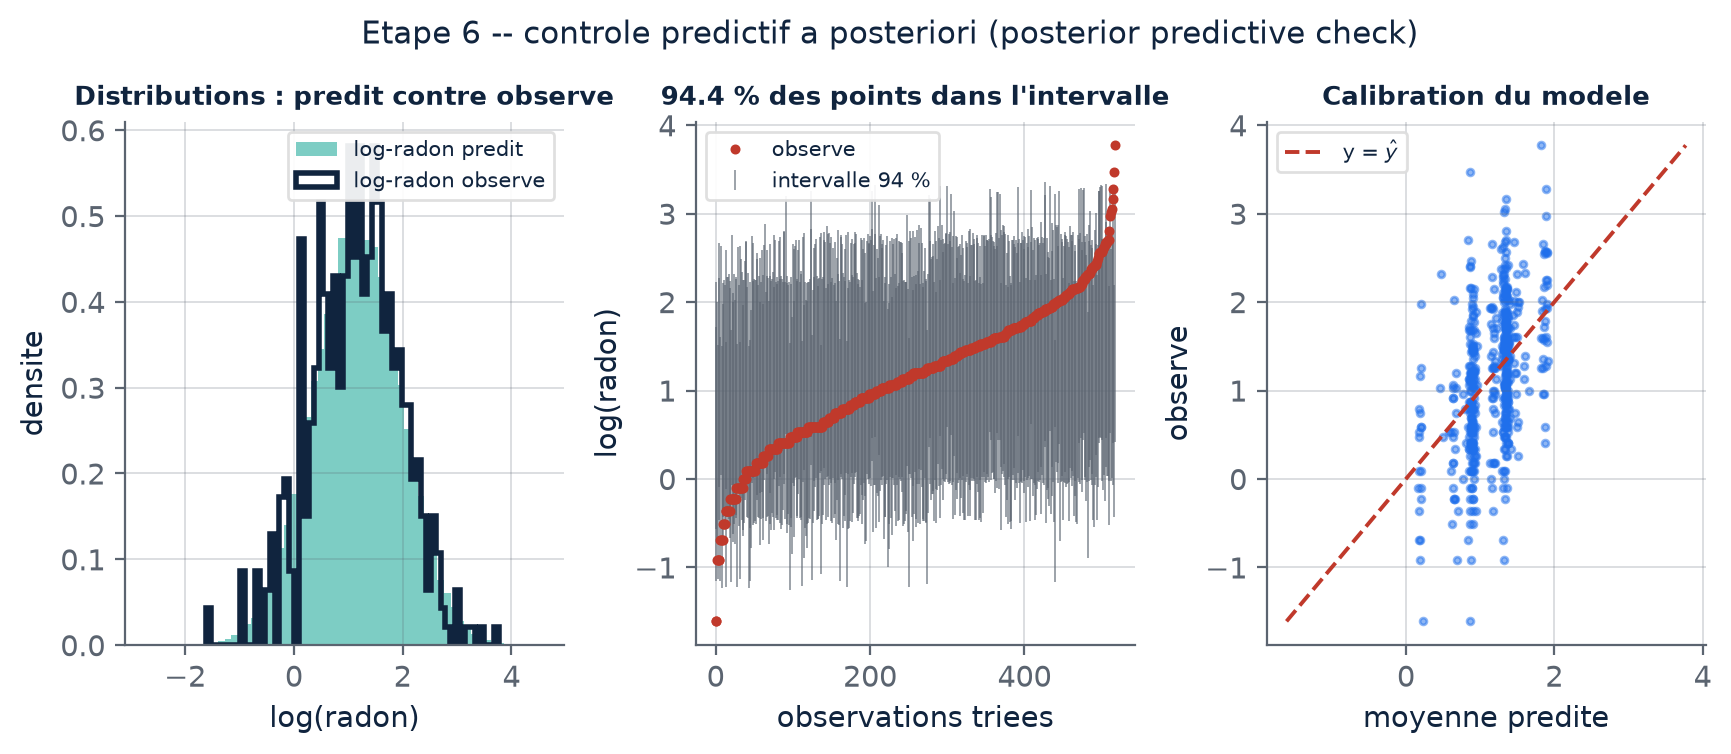
\includegraphics[width=.86\textwidth]{j11_ppc_radon.png}
\end{center}
\end{frame}

% [split]
\begin{frame}{Contrôle prédictif a posteriori : le modèle tient-il ses promesses ?}

\vspace{-1.5mm}
\begin{columns}[t]
\begin{column}{0.5\textwidth}
\begin{solbox}[Procédure et mesures (modèle radon, 1 200 tirages)]
\begin{enumerate}
  \item tirer $\tilde y^{(i)} \sim p(\tilde y \given \theta^{(i)})$ pour chaque
        tirage du posterior (2 000 réplications ici) ;
  \item comparer les \textbf{distributions} de $\tilde y$ et de $y$ ;
  \item compter la proportion d'observations couvertes par l'intervalle 94 \%.
\end{enumerate}
Mesures : couverture 94,4 \% ; moyenne observée 1,156 contre
1,156 prédite ; écart-type observé 0,805 contre
0,811 prédit.
\end{solbox}
\end{column}
\begin{column}{0.48\textwidth}
\begin{kbox}[Ce qu'un PPC révèle (et ne révèle pas)]
\begin{itemize}
  \item Il teste le \textbf{modèle} : forme de la vraisemblance, priors, effets
        oubliés. Un PPC raté n'est \emph{pas} un problème d'échantillonnage.
  \item Ici la couverture est proche du nominal et les moyennes coïncident :
        le log-radon par comté est raisonnablement décrit.
  \item Un excès de valeurs extrêmes observées signalerait des queues trop
        légères (passer à une Student, ou modéliser la surdispersion).
  \item Le PPC ne « prouve » pas que le modèle est vrai : il ne détecte que les
        incohérences qu'on a pensé à regarder.
\end{itemize}
\end{kbox}
\end{column}
\end{columns}
\end{frame}

% ---------------------------------------------------------------- 42
% [split]
\begin{frame}{Valider la chaîne contre une référence exacte}
\begin{center}
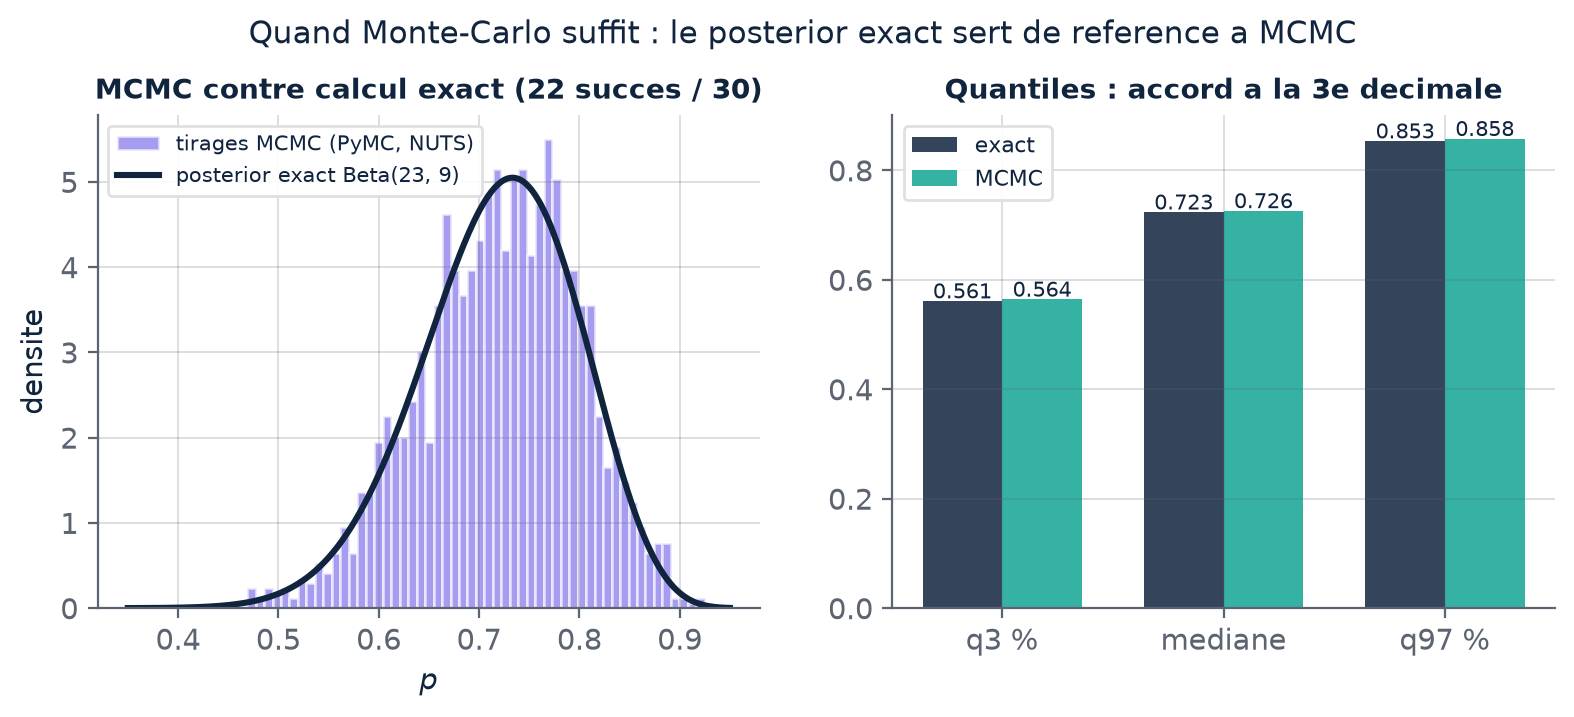
\includegraphics[width=\textwidth]{j14_mcmc_vs_exact.png}
\end{center}
\end{frame}

% [split]
% [suite5]
\begin{frame}{Valider la chaîne contre une référence exacte}
% [rogna]
\small
\begin{columns}[t]
\begin{column}{0.46\textwidth}
\begin{ebox}[Le test le plus simple qui vaut la peine]
On se place dans un cas où le posterior est \textbf{connu} : prior Beta$(1,1)$,
vues Binomiales, $k$ = 22 succès sur $n$ = 30 essais $\Rightarrow$
$p \given \data \sim \mathrm{Beta}(23, 9)$, donc
$\E[p \given \data] = 23/32 = 0{,}71875$.
\end{ebox}
\end{column}
\end{columns}
\end{frame}

% [suite5]
\begin{frame}{Valider la chaîne contre une référence exacte (suite)}
\begin{solbox}[Accord mesuré]
\footnotesize\begin{tabular}{@{}p{1.7cm}p{1.5cm}p{1.8cm}@{}}
\toprule
quantité & exact & MCMC (PyMC) \\
\midrule
moyenne & 0,71875 & 0,72067 \\
$q_{3\,\%}$ & 0,5610 & 0,5641 \\
médiane & 0,7234 & 0,7258 \\
$q_{97\,\%}$ & 0,8533 & 0,8576 \\
\midrule
$\hat R$ & --- & 1,00592 \\
ESS & --- & 593,7 \\
\bottomrule
\end{tabular}
\vspace{1mm}
\\ Écart absolu sur la moyenne : \textbf{0,00192}. La chaîne est donc
correcte ; tout écart restant est l'erreur de simulation elle-m\^eme.
\end{solbox}
\end{frame}

% ---------------------------------------------------------------- 43
\begin{frame}{Que faire quand ça ne converge pas : procédure ordonnée}
% [rogna]
\footnotesize
\begin{columns}[t]
\begin{column}{0.52\textwidth}
\begin{abox}[Procédure (dans cet ordre)]
\begin{enumerate}
  \item \textbf{Lire les avertissements} de PyMC mot à mot : ils nomment le
        problème (« 14 divergences after tuning », « ESS is extremely low »).
  \item \textbf{Contrôler les divergences} : si $> 0$, ne rien interpréter
        avant de les avoir supprimées.
  \item \textbf{Reparamétrer} : centrée $\rightarrow$ non centrée, échelles des
        prédicteurs, paramètres à contraintes (log, logit).
  \item \textbf{Augmenter \py{target\_accept}} (0,9 $\rightarrow$ 0,95
        $\rightarrow$ 0,99) : plus sûr, mais plus lent.
  \item \textbf{Allonger \py{tune}} et augmenter \py{init} (\py{"adapt\_diag"}) si
        le démarrage échoue.
  \item \textbf{Simplifier le modèle} : retirer un effet, remplacer une
        distribution, borner un prior.
  \item \textbf{Changer d'échantillonneur} en dernier recours : Gibbs si les
        conditionnelles sont closes, métropole à l'intérieur de Gibbs pour les
        variables discrètes.
\end{enumerate}
\end{abox}
\end{column}
\begin{column}{0.46\textwidth}
\begin{wbox}[Les trois erreurs qui font perdre une journée]
\nok{} \textbf{Augmenter les tirages} alors que le problème est géométrique :
le $\hat R$ ne bougera pas.\\[1mm]
\nok{} \textbf{Supprimer le burn-in} pour « nettoyer » un $\hat R$ élevé :
il ne mesure qu'après la chauffe, cela ne change rien.\\[1mm]
\nok{} \textbf{Thinner} pour faire baisser l'autocorrélation : l'ESS de ce qui
reste est identique, on a juste jeté des tirages.
\end{wbox}
\begin{kbox}[Le réflexe qui marche]
Dans 80 \% des cas de non-convergence sur un modèle hiérarchique, la cause est
l'écriture \emph{centrée} (slide 30) : passer en non centré fait tomber les
divergences de 17 à 0 et multiplie l'ESS par 8 sur notre exemple.
\end{kbox}
\end{column}
\end{columns}
\end{frame}

% ---------------------------------------------------------------- 44
\begin{frame}{Synthèse 5.4 --- Diagnostics et validation}
\begin{columns}[t]
\begin{column}{0.49\textwidth}
\begin{tcolorbox}[enhanced,colback=byPurple!7,colframe=byPurple,arc=2mm,
   title={\bfseries\color{white}\faLightbulb\ Synthèse},colbacktitle=byPurple,
   attach boxed title to top left={xshift=3mm,yshift=-2mm},
   boxed title style={arc=1mm,boxrule=0pt}]
\begin{itemize}
  \item \textbf{Trace} : qualitatif, détecte la non-stationnarité. À regarder en
        premier, à ne jamais confondre avec une preuve.
  \item \textbf{Rank plot} : le seul outil visuel qui voit un mode manqué.
  \item \textbf{$\hat R < 1{,}01$} sur \emph{tous} les paramètres : mesuré à
        1,00311 sur le modèle radon.
  \item \textbf{ESS} : le nombre de tirages utiles ; sous 100, aucun intervalle
        n'est fiable. À comparer au coût (ESS par évaluation de gradient).
  \item \textbf{Divergences} : zéro, ou rien d'autre. Mesuré : 17 en paramétrisation
        centrée, 0 en non centrée.
  \item \textbf{PPC} : valide le \emph{modèle}, pas la chaîne --- et c'est une
        étape obligatoire avant toute décision.
  \item \textbf{Validation} : quand un posterior exact existe, comparer (accord
        à la 3\ieme{} décimale obtenu ici).
\end{itemize}
\end{tcolorbox}
\end{column}
\begin{column}{0.49\textwidth}
\begin{qbox}[Quiz de diagnostic -- que concluez-vous ?]
\textbf{Cas A.} $\hat R$ = 1,004 ; ESS = 38 pour $b$ ; 0 divergence.
\\ \footnotesize Convergence apparente mais précision insuffisante : allonger la
chaîne ou améliorer la géométrie.\\[1.5mm]
\textbf{Cas B.} $\hat R = 1{,}00$ ; ESS = 1 200 ; 3 divergences sur 4 000.
\\ \footnotesize Le plus dangereux : tout semble parfait, mais 3 zones du
posterior n'ont pas été explorées. Reparamétrer et relancer.\\[1.5mm]
\textbf{Cas C.} Tous les diagnostics sont parfaits, mais le PPC donne une
couverture de 71 \% pour un intervalle annoncé à 94 \%.
\\ \footnotesize La chaîne est bonne, le \emph{modèle} est faux : ajouter un effet
ou changer la vraisemblance.\\[1.5mm]
\textbf{Cas D.} Les deux chaînes donnent $\bar\theta$ = 0,31 et 0,72, $\hat R$ = 2,4.
\\ \footnotesize Deux modes, chaînes initialisées de part et d'autre : la multimodalité
doit être traitée dans le modèle (ou par échantillonnage par tempérage), pas par
plus de tirages.
\end{qbox}
\end{column}
\end{columns}
\end{frame}

% ---------------------------------------------------------------- 45
\begin{frame}{Mini-projet guidé : le radon du Minnesota (section 5.5)}
% [rogna]
\small
\begin{columns}[t]
\begin{column}{0.52\textwidth}
\begin{ebox}[Les données, et la question posée]
Fichier \file{src/data/srrs2.dat} (10\,000 lignes d'origine, 919 mesures du
Minnesota). On retient les \textbf{12 comtés les plus mesurés} :
\begin{itemize}
  \item 518 mesures, 12 comtés ;
  \item 65 logements au premier étage, 453 en sous-sol ;
  \item concentration en radon : moyenne \textbf{1,1558} en log(pCi/L),
        écart-type 0,805 ;
  \item 7 \% des mesures dépassent 10 pCi/L, le seuil d'action
        de l'agence américaine (log(10) = 2,3026) ;
  \item moyenne brute : premier étage 0,606 contre sous-sol 1,235,
        soit une différence de -0,629 en log, c'est-à-dire
        $\exp(-0{,}629) = 0{,}53$.
\end{itemize}
\textbf{Question :} l'effet « premier étage » est-il réel et de quelle taille,
comté par comté ?
\end{ebox}
\end{column}
\begin{column}{0.46\textwidth}
\begin{abox}[Grille d'évaluation notée (20 points)]
\footnotesize\begin{tabular}{@{}p{4.8cm}r@{}}
\toprule
étape & points \\
\midrule
1. Formulation probabiliste complète, variables et indices & 2 \\
2. Justification des priors (échelle, ordre de grandeur) & 3 \\
3. Vérification prédictive \emph{a priori} et critique du prior & 2 \\
4. Échantillonnage reproductible (graines, taille, réglages) & 3 \\
5. Diagnostics \emph{complets} et interprétés (trace, $\hat R$, ESS, divergences) & 5 \\
6. Contrôle prédictif \emph{a posteriori} & 2 \\
7. Décision chiffrée avec intervalle et restitution écrite & 3 \\
\midrule
total & 20 \\
\bottomrule
\end{tabular}
\vspace{1mm}
\\
\footnotesize Les points 5 et 2 sont les plus discriminants : un modèle qui
« tourne » sans diagnostics interprétés ne vaut pas la moitié du barème.
\end{abox}
\end{column}
\end{columns}
\end{frame}

% ---------------------------------------------------------------- 46
% [split]
\begin{frame}{Étapes 1 à 3 : formulation, priors et vérification \emph{a priori}}
\begin{center}
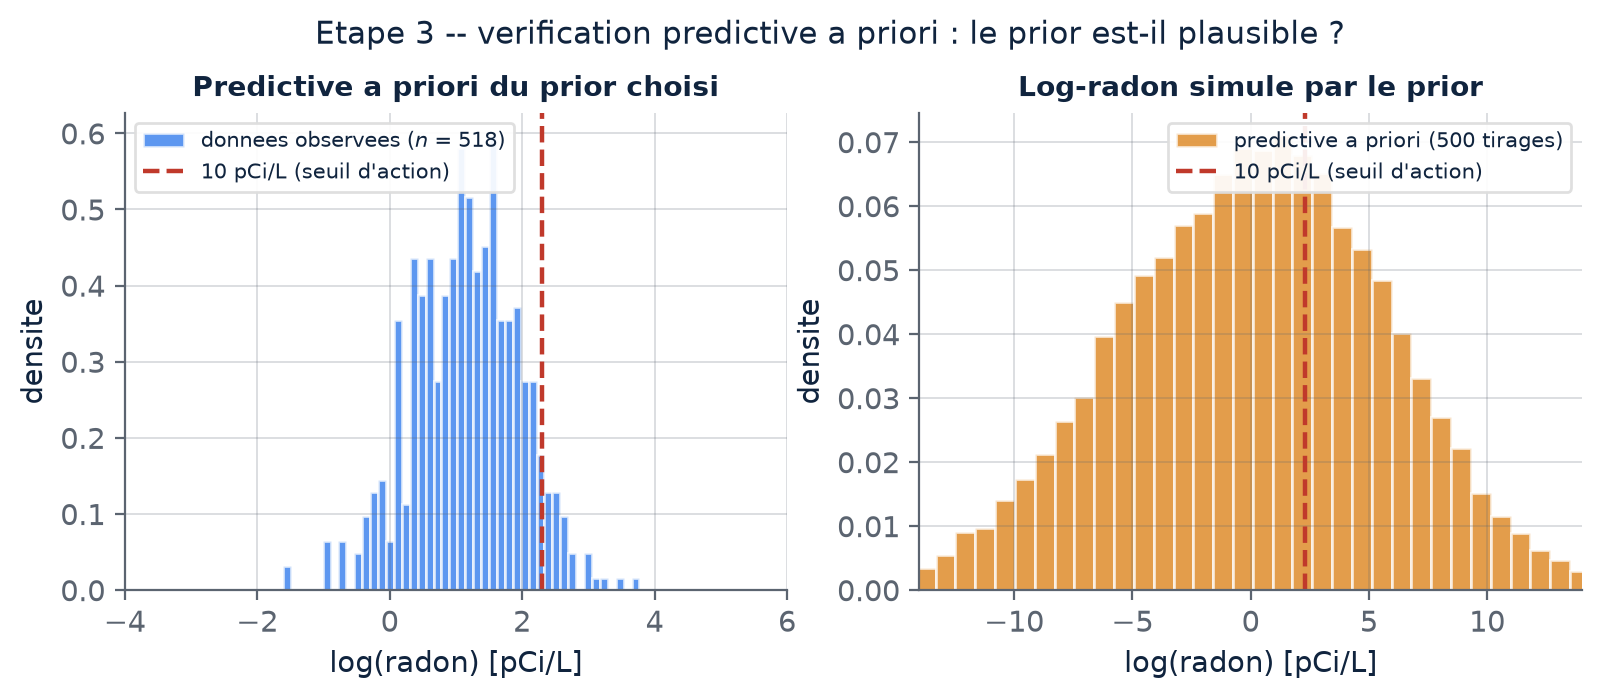
\includegraphics[width=\textwidth]{j13_prior_predictive.png}
\end{center}
\end{frame}

% [split]
% [suite]
\begin{frame}{Étapes 1 à 3 : formulation, priors et vérification \emph{a priori}}
% [rogna]
\footnotesize
\begin{columns}[t]
\begin{column}{0.52\textwidth}
\begin{ebox}[Étape 1 --- le modèle]
Notations : $y_{ij}$ = log-radon du logement $i$ du comté $j$ ;
$x_{ij} = 1$ si premier étage, $0$ sinon.
\[
y_{ij} \given a_j, b, \sigma_y \sim \N\!\big(a_j + b\,x_{ij},\; \sigma_y^2\big),
\qquad
a_j \given \mu_a, \sigma_a \sim \N(\mu_a, \sigma_a^2).
\]
Trois niveaux d'incertitude : le bruit $\sigma_y$, les écarts de comtés
$\sigma_a$, la moyenne générale $\mu_a$. C'est le modèle de Gelman--Hill
simplifié, et c'est un \textbf{modèle hiérarchique} : les comtés empruntent de
l'information à l'ensemble.
\end{ebox}
\end{column}
\begin{column}{0.46\textwidth}

\vspace{-2mm}
\begin{solbox}[Étape 3 — critique du prior]
500 simulations du prior : les log-radon simulés couvrent une plage
\emph{beaucoup plus large} que les données (de -13,34 à 13,25 aux
quantiles 1--99 \%), et 35,9 \% des valeurs simulées dépasseraient
10 pCi/L alors que les données sont à 7 \%.
\\[1mm]
Aucun prior n'exclut les données observées : ils sont \textbf{faiblement
informatifs mais pas absurdes}. Une telle vérification aurait invalidé un prior
comme $\N(0, 0{,}1)$ sur $\mu_a$.
\end{solbox}
\end{column}
\end{columns}
\end{frame}

% [suite]
\begin{frame}{Étapes 1 à 3 : formulation, priors et vérification \emph{a priori} (suite)}
\begin{kbox}[Étape 2 --- les priors, et pourquoi]
\footnotesize\begin{tabular}{@{}p{1.2cm}p{1.7cm}p{2.8cm}@{}}
\toprule
paramètre & prior & justification \\
\midrule
$\mu_a$ & $\N(0, 5)$ & log-radon plausible entre $-15$ et $+15$ \\
$\sigma_a$ & HalfNormal$(2)$ & dispersion inter-comtés de l'ordre de 1-2 \\
$b$ & $\N(0, 3)$ & effet d'étage plausible, large mais borné \\
$\sigma_y$ & HalfNormal$(2)$ & bruit résiduel de l'ordre de 1 \\
\bottomrule
\end{tabular}
\end{kbox}
\end{frame}

% ---------------------------------------------------------------- 47
\begin{frame}[fragile]{Étape 4 : l'échantillonnage, en quinze lignes}
\begin{columns}[t]
\begin{column}{0.55\textwidth}
\begin{codebox}[modele\_radon.py --- exécuté (PyMC 5.28, NUTS, 2 chaînes)]
\begin{lstlisting}[basicstyle=\ttfamily\fontsize{5.8}{6.6}\selectfont]
import pymc as pm, arviz as az
with pm.Model() as modele:
    mu_a    = pm.Normal("mu_a", 0.0, 5.0)
    sigma_a = pm.HalfNormal("sigma_a", 2.0)
    b       = pm.Normal("b", 0.0, 3.0)
    a       = pm.Normal("a", mu_a, sigma_a, shape=12)
    sigma_y = pm.HalfNormal("sigma_y", 2.0)
    pm.Normal("y", mu=a[idx] + b * x, sigma=sigma_y, observed=y)

    idata = pm.sample(draws=1000, tune=1000, chains=2,
                      cores=1, target_accept=0.9,
                      random_seed=7, progressbar=False)
    pm.sample_posterior_predictive(
        idata, extend_inferencedata=True)
\end{lstlisting}
\end{codebox}
\end{column}
\begin{column}{0.43\textwidth}
\begin{solbox}[Ce que produit cette exécution]
\footnotesize\begin{tabular}{@{}p{3.4cm}p{1.9cm}@{}}
\toprule
& mesure \\
\midrule
durée totale & 655 s \\
tirages (hors chauffe) & 1 200 ($2 \times 600$) \\
pas de NUTS au total & 8 520 \\
acceptation moyenne & 0,903 \\
divergences & 0 \\
$\hat R_{\max}$ & 1,00311 \\
ESS minimal & 872 \\
\bottomrule
\end{tabular}
\vspace{1.5mm}
\\ Pas de compilateur C sur cette machine : PyTensor tourne en Python pur. D'où
le choix de \py{cores=1}, de 2 chaînes et de 1 000 tirages --- contrainte
matérielle \textbf{déclarée} dans le rapport, pas dissimulée.
\end{solbox}
\end{column}
\end{columns}
\end{frame}

% ---------------------------------------------------------------- 48
\begin{frame}{Étape 5 : diagnostics du modèle radon, chiffre par chiffre}
% [rogna]
\small
\begin{center}
\footnotesize
\begin{tabular}{@{}p{2.9cm}p{2.2cm}p{2.2cm}p{4.9cm}@{}}
\toprule
\textbf{Paramètre} & \textbf{moyenne} & \textbf{IC 94 \%} & \textbf{Lecture} \\
\midrule
$\mu_a$ (moyenne des comtés) & 1,417 & [1,189 ; 1,668] &
log-radon moyen d'un sous-sol, toutes régions confondues \\[1.5mm]
$\sigma_a$ (dispersion) & 0,405 & [0,252 ; 0,678] &
les comtés diffèrent, mais modérément \\[1.5mm]
$b$ (premier étage) & -0,700 & [-0,896 ; -0,520] &
facteur 0,50 : le premier étage divise le radon par 2 \\[1.5mm]
$a_j$ (12 comtés) & 0,882 à 1,889 & --- &
les extrêmes bruts sont ramenés vers la moyenne \\[1.5mm]
$\sigma_y$ (bruit) & 0,720 & --- &
variabilité entre logements d'un même comté \\
\bottomrule
\end{tabular}
\end{center}
\vspace{1mm}
\begin{columns}[t]
\begin{column}{0.5\textwidth}
\begin{kbox}[Ce que ces nombres racontent]
L'effet de l'étage vaut $b = $ -0,700 en log : les logements du premier étage
ont $\exp(-0,700) = 0,497$ fois la concentration d'un sous-sol, soit environ
moitié moins. L'intervalle [-0,896 ; -0,520] exclut clairement 0 : l'effet est réel.
La dispersion inter-comtés $\sigma_a$ = 0,405 est petite devant l'étendue
des moyennes \emph{brutes} des comtés.
\end{kbox}
\end{column}
\begin{column}{0.5\textwidth}
\begin{wbox}[Ce que ces nombres ne disent pas]
Il ne s'agit \textbf{pas} d'un effet causal : la variable « étage » est corrélée à
l'âge du b\^atiment, à la géologie et au type de construction, non mesurés ici.
Le modèle quantifie une association, avec son incertitude --- rien de plus.
\end{wbox}
\end{column}
\end{columns}
\end{frame}

% ---------------------------------------------------------------- 49
% [rogna]
% [rogna]
% [rogna]
% [split]
\begin{frame}{Étape 6 : prédiction, décision et restitution}
\begin{center}
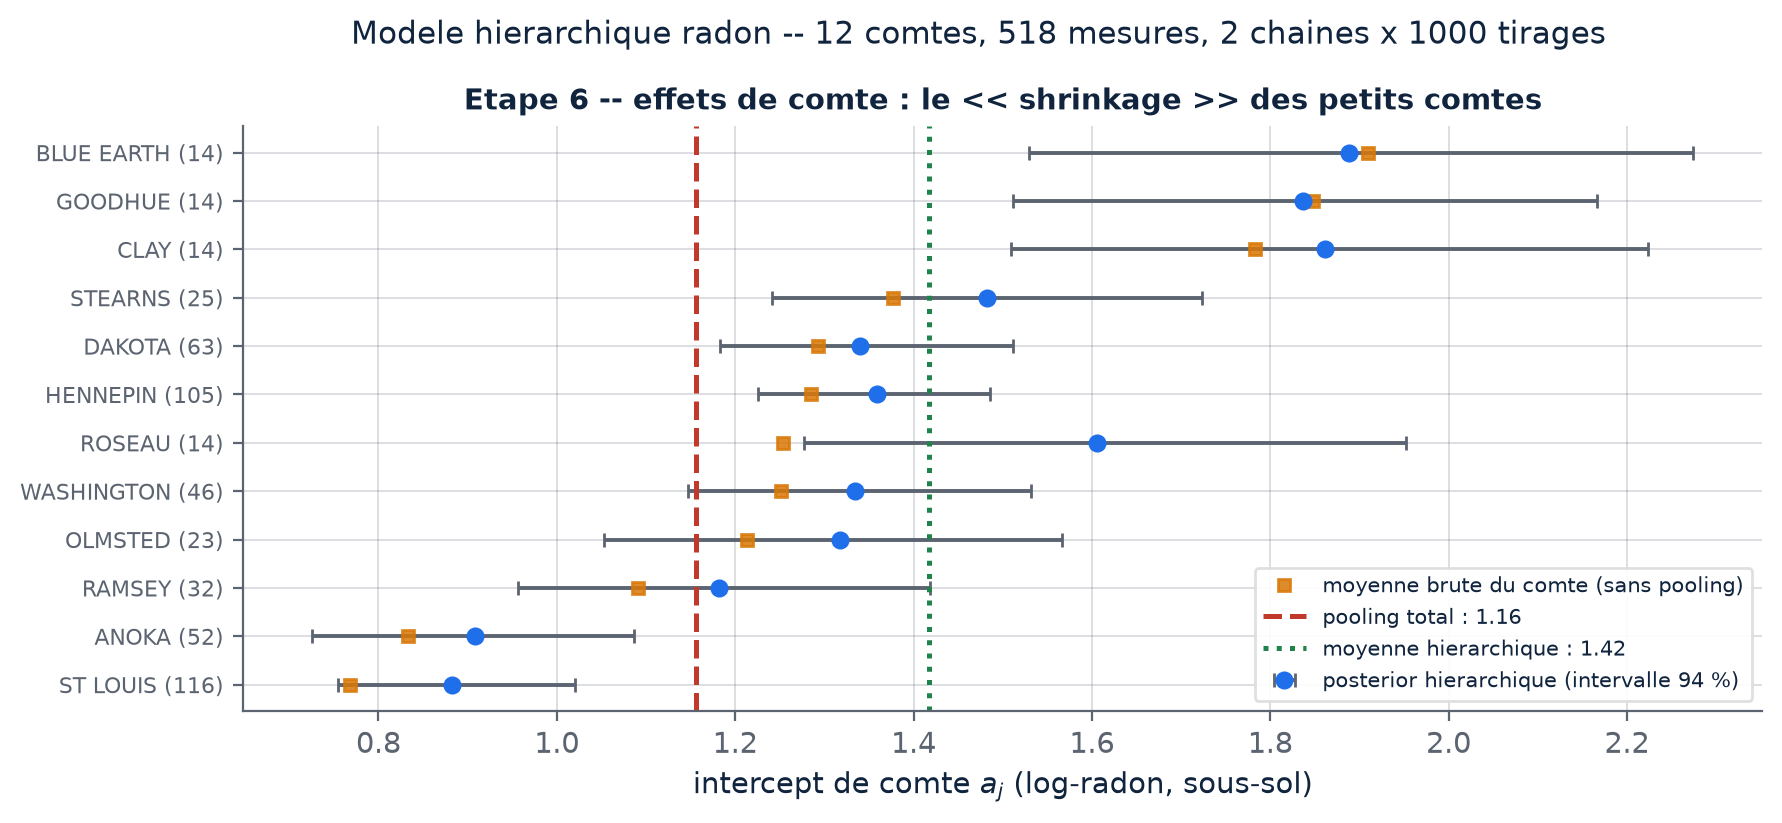
\includegraphics[width=.86\textwidth]{j12_forest_radon.png}
\end{center}
\end{frame}

% [split]
\begin{frame}{Étape 6 : prédiction, décision et restitution}

\vspace{-1.5mm}
\begin{columns}[t]
\begin{column}{0.52\textwidth}
\begin{solbox}[Le \emph{shrinkage}, mesuré]
\begin{itemize}
  \item Moyennes brutes : de 0,768 à 1,909 selon le comté.
  \item Après hiérarchie : de 0,882 à 1,889 : les comtés à
        petit effectif sont \textbf{ramenés vers la moyenne générale}
        (1,156).
  \item C'est ce qui rend le modèle hiérarchique supérieur à la comparaison de
        12 modèles séparés : chaque comté emprunte de la force aux autres.
\end{itemize}
\end{solbox}
\end{column}
\begin{column}{0.46\textwidth}
\begin{abox}[La décision qu'on ose écrire]
Avec $\hat b = $ -0,700 et un IC 94 \% de [-0,896 ; -0,520] :
\begin{quote}\small
« \textbf{Le premier étage divise la concentration médiane en radon par environ
2,0 par rapport à un sous-sol} (intervalle de crédibilité 94 \%
[1,68 ; 2,45]). Cette conclusion repose sur un modèle hiérarchique validé par ses
diagnostics ($\hat R_{\max}$ = 1,00311, 0 divergence) et par un contrôle
prédictif couvrant 94,4 \% des observations. »\end{quote}
C'est le format de restitution attendu au mini-projet : \textbf{un chiffre, un
intervalle, une phrase de portée}.
\end{abox}
\end{column}
\end{columns}
\end{frame}

% ---------------------------------------------------------------- 50
% [suite5]
\begin{frame}{Synthèse du chapitre 5 --- et ce que vous savez faire maintenant}
\begin{columns}[t]
\begin{column}{0.52\textwidth}
\begin{tcolorbox}[enhanced,colback=byPurple!7,colframe=byPurple,arc=2mm,
   title={\bfseries\color{white}\faLightbulb\ Les huit idées du chapitre},
   colbacktitle=byPurple,
   attach boxed title to top left={xshift=3mm,yshift=-2mm},
   boxed title style={arc=1mm,boxrule=0pt}]
\begin{enumerate}
  \item On ne calcule plus l'intégrale de Bayes : on la \textbf{simule}
        (erreur en $1/\sqrt N$, mesurée à la pente $-0{,}501$).
  \item Un noyau de transition invariant pour $\pi$ suffit à échantillonner :
        \textbf{bilan détaillé}.
  \item Metropolis-Hastings accepte avec $\min(1, \text{rapport})$ : la constante
        de normalisation disparaît.
  \item La proposition est le seul curseur (ESS optimal mesuré à $s$ = 0,35) et
        les tirages restent \textbf{corrélés} (ESS = 5 896 sur 30 000).
  \item Gibbs est exact et sans réglage, HMC utilise le gradient, NUTS choisit
        la longueur : ESS/\,itér.\ mesurés 0,167 / 1,000 / 0,162.
  \item Les \textbf{divergences} sont le symptôme de la mauvaise géométrie :
        17 en centré, 0 en non centré.
  \item \textbf{Trace, rank plot, $\hat R < 1{,}01$, ESS $> 400$, 0 divergence} :
        la liste de contrôle minimale.
  \item Le \textbf{PPC} valide le modèle, pas l'échantillonneur.
\end{enumerate}
\end{tcolorbox}
\end{column}
\begin{column}{0.46\textwidth}
\begin{abox}[Livrable du mini-projet]
Un notebook ou un script reproduisant les 6 étapes sur les données radon, avec :
les priors justifiés, la vérification \emph{a priori}, la sortie d'échantillonnage
(reproductible : graine et version), les diagnostics \emph{interprétés}, le PPC, et
une phrase de décision chiffrée. \textbf{20 points}, grille détaillée slide 45.
\end{abox}
\vspace{1mm}
\end{column}
\end{columns}
\end{frame}

% [suite5]
\begin{frame}{Synthèse du chapitre 5 --- et ce que vous savez faire maintenant (suite)}
\begin{kbox}[Pour aller plus loin]
\begin{itemize}
  \item \textbf{Chapitre 4} pour la comparaison de modèles (WAIC, LOO-CV) sur ce
        m\^eme jeu de données.
  \item \textbf{TP5} : \file{notebooks/TP5\_mcmc\_\allowbreak diagnostics.ipynb} ;
        squelette du projet : \file{notebooks/PROJET\_\allowbreak modele\_hierarchique\_radon.ipynb}.
  \item Échantillonnage par tempérage, quasi-Monte-Carlo, MCMC variationnel
        (VI) : les outils qui prennent le relais quand NUTS reste trop lent.
\end{itemize}
\end{kbox}
\end{frame}

\end{document}
